\input{/Users/daniel/github/config/preamble-book.sty}
\input{/Users/daniel/github/config/thms-eng.sty}%This is available at github.com/danimalabares/config
\usepackage{textgreek}
\title{math}
\author{\href{https://github.com/danimalabares/math}{github.com/danimalabares/math}}

\begin{document}
\bibliographystyle{alpha}

\maketitle
\phantomsection
\tableofcontents
\clearpage
\chapter{basic math}

\section{adjoint}

for a linear map \(A\) we want to define its \textit{\textbf{adjoint}}
\[A:V \to W, \qquad A^{\dag}:W \to V\]
satisfying
\[\left<Av,w\right>_W=\left<v,A^\dag w\right>_V\]
so we need some matrices \(H\) and \(G\) for the metrics on \(W\) and \(V\). the latter equation is just
\[v^{\mathbf{T}}A^{\mathbf{T}}Hw=(Av)^{\mathbf{T}}Hw=v^{\mathbf{T}}GA^\dag w\]
where the \(\mathbf{T}\) is the usual transpose. so you conclude
\[A^{\mathbf{T}}H=GA^\dag \implies A^\dag:=G^{-1}A^{\mathbf{T}}H\]

this in fact allows to define \textit{\textbf{frobenius norm}} by
\[\|A\|^2=\operatorname{tr}A^\dag A=\operatorname{tr}G^{-1}A^{\mathbf{T}}HA\]

but you can also smooth the construction to get that 

\section{trace}

I need to be sure I know what is the trace. The \textit{\textbf{trace}} of an endomorphism \(A \in \operatorname{End}(V)\) is the sum of the diagonal entries of \(A\) with respect to any basis. So I claim that this number is invariant under change of basis and prove it:

trace is commutative: \(\operatorname{tr}(AB)=\operatorname{tr}(BA)\) because is just multiplication of some numbers. Change of coordinates is a multiplication of matrices, can commute, get identity, done.

\textit{Warning: confusion up ahead} choose two bases \(e_i\) and \(e'_i\) of \(V\). Define
\[Ae_i=A^j_ie_j,\qquad Ae'_i=\tilde{A}^j_ie'_j,\qquad e_i=J^j_ie'_j, \qquad e'_i=\overline{J}^j_ie_j\]
so the claim is that
\[A^i_i=\tilde{A}^i_i\]

Change of coordinate basis does
\[A^i_j=J^k_i \tilde{A}^j_k \overline{J}^\ell_j\]
(the index names on LHS and RHS aren't related) because for any basic vector \(e_i\),
\[Ae_i=A^j_i e_j=A^j_i J^k_j e'_k=J_i^jA_j^ke'_k=J_i^jA_j^k \overline{J}_k^\ell e_\ell\]
So
\[\operatorname{tr}J\tilde{A}J^{-1}\overset{\operatorname{def}}{=}J^k_i\tilde{A}^j_k J^\ell_k=A^i_i \overset{\operatorname{def}}{=}\operatorname{tr}A\]


\section{tensor product}

\begin{defn}[Tensor product by \cite{sea}]\leavevmode
If \(V\) and \(W\) are \(R\)-modules and \(R\) is a ring, I think of the \textit{\textbf{tensor product}} as
\[V\otimes W:=\left\{\sum_{\text{finite} }\lambda_i (v \otimes w)_i, v \in V, w \in W \right\} \Big/ \substack{\begin{array}{c}v \otimes (w_1+w_2)\sim v\otimes w_1+ v\otimes w_2\\ (v_1+v_2) \otimes w \sim(v_1 \otimes w)+(v_2 \otimes w)\\ \lambda(v \otimes w)\sim(\lambda v) \otimes w \sim  v \otimes(\lambda v)\end{array}}\]
More formally, the free \(R\)-module generated by \(V \times W\) (we say this so that things of the kind \(\lambda(v,w)\) make sense) quotiented by the ideal generated by these guys:
\begin{gather*}(v,w_1+w_2)-(v,w_1)-(v,w_2),\\ (v_1+v_2,w)-(v_1,w)-(v_2,w),\\ (\lambda v,w)-\lambda(v,w),\\(v,\lambda w)-\lambda(v,w)\end{gather*}
So that we denote the projection of \((v,w)\) by \(v \otimes w\). Also never forget that the product was defined when you have a product and Vakil has a product…
\begin{thing7}{and I have a product…}[Universal property of product]\leavevmode
It's actually nice to recall that any two objects satisfying the ``every map of such kind factors through a map involving the product"-property, you can construct an isomorphism between them. So the only thing satisfying the product property is the product.
\end{thing7}
\end{defn}
And of course you must understand the construction of tensor product using universal property. Suppose you have a tensor product…

\begin{remark}\leavevmode
Maybe when I think of \(\operatorname{span}\) of some set of symbols I mean the free \(R\)-module generated by the (as many symbols I need)-th product of the place where the symbols live, quotiented by the obvious linearlity relations.
\end{remark}

\begin{remark}\leavevmode
The difference between tensor product and cartesian product is that the latter is not bilinear in addition and scalar multiplication, look:
\begin{align*}
	(v_1,w_1)+(v_2,w_2)&=(v_1+v_2,w_1+w_2),\\
	\lambda(v,w)&=(\lambda v, \lambda w)
\end{align*}
\end{remark}

\begin{thing6}{14.3.6, \cite{sea}}[Tensor algebra constructions]\leavevmode
Let \(M\) be an \(A\)-module. The \textit{\textbf{tensor algebra}} \(T^\bullet(M)\) is just (the direct sum, probably) of \(T^0(M):=A\), \(T^n(M):=\underbrace{M\otimes_A \ldots\otimes_A M}_{n\text{ times} }\).

The \textit{\textbf{symmetric algebra}} \(\operatorname{Sym}^\bullet(M)\) is the quotient of \(T^\bullet (M)\) by the (two-sided) ideal generated by all the elements of the form \(x \otimes y -y \otimes x\). So,
\[\operatorname{Sym}^n(M)=M \otimes \ldots \otimes M \Big/m_1 \otimes \ldots \otimes m_n - m_1' \otimes \ldots \otimes m_n'\]
where \((m_1',\ldots,m_n')\) is a rearrangement of \((m_1,\ldots,m_n)\).

Finally the \textit{\textbf{exterior algebra}} \(\Lambda^{\bullet}(M)\) is defined to be the quotient of \(T^\bullet M\) by the (two-sided) ideal generated by all the elements of the form \(x \otimes x\) for all \(x \in M\). Which implies that \(a \otimes b = -b \otimes a\) (Pf. do \((a+b) \otimes (a+b)\), but only if \(\operatorname{char}\neq 2\) right?) Apparently this gives you that
\[\Lambda^{n}M=\text{quotient of no sé que with a permutation} \]
Anyway I can finally say that if \(\mathcal{F}\) is a locally free rank-\(m\) sheaf, I can define \(T^n \mathcal{F}\), \(\operatorname{Sym}^n\mathcal{F}\) and \(\Lambda^{n}\mathcal{F}\), that will be locally free (exercise, and find their ranks, exercise). And just to conclude for today, the \textit{\textbf{determinant (line) bundle}} is  \(\Lambda^{\operatorname{rk}\mathcal{F}}\mathcal{F}:=\det\mathcal{F}\).
\end{thing6}
So why all this. Because adjunction formula gives you that the canonical bundle of the submanifold is \(K_{\text{ambient mfd}}\otimes_{\mathbb{C}?} \det \mathcal{N}\) where \(\mathcal{N}\) is the normal bundle of the submanifold which is the cokernel sheaf/bundle of the inclusion. So that's that.

\begin{thing7}{Plücker embedding}\leavevmode
It's a way to put Grassman inside a projective space:
\[\operatorname{Gr}(V,k) \hookrightarrow \mathbb{P}\Lambda^{k}V = \operatorname{Gr}(\Lambda^{k}V,1)\]
evidently given by
\[\text{basis } e_1,\ldots,e_k\text{ of \(U \in \operatorname{Gr}(V,k)\)}\longmapsto \operatorname{span}\{e_1 \wedge \ldots \wedge e_k\}\]


\end{thing7}




\section{sheaves}
\begin{table}[h!]
\centering
\renewcommand{\arraystretch}{1.3}
\begin{tabular}{|l|c|}
\hline
\textbf{Propriedade do feixe \( \mathcal{F} \)} & \textbf{Pode ser verificada nos stalks?} \\
\hline
\( \mathcal{F} = 0 \) & Sim \\
\( \varphi: \mathcal{F} \to \mathcal{G} \) é mono/epi/iso & Sim \\
Sequência exata & Sim \\
\( \operatorname{Supp}(\mathcal{F}) \) & Sim \\
\( \mathcal{F}_x \) plano/torsion-free & Sim (se feixe quasi-coerente) \\
Localmente livre de posto \( r \) & Sim \\
\hline
Localmente finitamente gerado & \textbf{Não} \\
Quasi-coerência / coerência & \textbf{Não} \\
Ser um feixe (vs. pré-feixe) & \textbf{Não} \\
Geração global por seções & \textbf{Não} \\
\hline
\end{tabular}
\caption{Propriedades de feixes verificáveis nos stalks}
\end{table}

\subsection{what's a sheaf}
a functor from \(\operatorname{Open} \to \operatorname{Ab} \).

\subsection{cech cohomology}

the point is that

a \textit{\textbf{0-cech cocycle}} is the assignment of a section \(f_\alpha\) to every open set \(U_\alpha\) of the cover. Every global section gives you a \(0\)-cocycle by restriction, and that turns out to be an isomorphism. So global sections are in fact \(H^0\).

a  \textit{\textbf{1-cech cocycle}} is the assignment of a function \(g_{\alpha \beta}:U_\alpha \cap U_\beta \to k\) satisfying the cocycle property. so it's a line bundle, and \(H^1=\operatorname{Pic}\).

\begin{question}\leavevmode
\(\mathsf{OK}\) but when we say that a 0-cech cocycle is the assignment of a section \(f_\alpha\) to every open set I think well, that's a divisor, a hypersurface, i think; it's a line bundle; because you define the manifold to be the zero-locus of these functions; haha but no: that's just a random assignment of functions and has no structure a priori.

what gives you a hypersurface is when these two functions can be glued together, and that's the condition that \(f_\alpha/f_\beta \in \mathsf{GL}(U_\alpha \cap U_\beta,k)\). now that's a line bundle. and also: \textbf{it's a {\color{2}1}-cocycle}.
\end{question}

\subsection{some other stuff i learnt while learning}

\(\mathfrak{m}_x \subset C^\infty(\mathbb{R}^n)\) is the ideal of smooth functions vanishing at \(x \in \mathbb{R}^n\). In \cite{hart} definition of \textit{\textbf{local ring of \(P\) in \(Y\)}}, which is the ring of germs of regular functions of the variety \(Y\) at the point \(P\), that it is a local ring with maximal ideal \(\mathfrak{m}\), the set of germs of regular functions which vanish at \(P\). The residue field is \(k\).

\begin{exercise}\leavevmode
Show that indeed \(\mathfrak{m}_x\), the ideal of functions vanishing at \(x\), is maximal.
\end{exercise}
\begin{proof}[Solution]\leavevmode
	Suppose that \(\mathfrak{n} \supseteq \mathfrak{m}_x\) is another ideal contained in \(\mathcal{O}_{X,x}\). If \([f] \in \mathfrak{n}\) does not vanish at \(x\), then we can do \([1/f]\) very near  \(x\), giving \([f][1/f] \in \mathfrak{n}\), so that \(\mathfrak{n}=\mathcal{O}_{X,x}\). And if all \([f] \in \mathfrak{n}\) vanish at \(x\), we get \(\mathfrak{n}=\mathfrak{m}_x\).
\end{proof}

\begin{thing6}{Little discussion with GPT}\leavevmode
In differential geometry we have the sheaf \(\mathcal{F}\) of smooth functions. That's like the scalars of some other structure that we build over it: the tangent sheaf, which is defined as derivations on \(\mathcal{F}(U)\). Remember that for any sheaf \(\mathcal{F}\), the elements of \(\mathcal{F}(U)\) are called sections. Yes, the sections of the tangent bundle are vector fields.

(The proof that \(\mathcal{T}_M\), the tangent sheaf, is a locally free \(\mathcal{F}\)-module (and thus a vector bundle) is just showing that \(\partial_i\) are basis of \(\mathcal{F}(U)\).)

The \textbf{tangent bundle} $TM$ of a smooth manifold $M$ is a vector bundle whose dual, the \textbf{cotangent bundle} $T^*M$, is locally generated by differentials $dx^i$.

	In algebraic geometry, we have an analogous structure:

\begin{itemize}
  \item The \textbf{structure sheaf} $\mathcal{O}_X$ assigns to each open set $U \subseteq X$ the ring of regular functions on $U$.
  \item The \textbf{sheaf of Kähler differentials} $\Omega^1_X$ is the analogue of the cotangent bundle: it is an $\mathcal{O}_X$-module generated by formal differentials $df$.
  \item The \textbf{tangent sheaf} $\mathcal{T}_X$ is the dual of $\Omega^1_X$, i.e.,
  \[
  \mathcal{T}_X := \mathcal{H}om_{\mathcal{O}_X}(\Omega^1_X, \mathcal{O}_X),
  \]
  and it corresponds to derivations of the structure sheaf:
  \[
  \mathcal{T}_X(U) = \operatorname{Der}_{\mathbb{K}}(\mathcal{O}_X(U), \mathcal{O}_X(U)).
  \]
  \item These sheaves are \textbf{quasicoherent sheaves}, which generalize vector bundles to the algebraic setting.
\end{itemize}

So, quasicoherent sheaves play the role of vector bundles in algebraic geometry, and in particular, $\mathcal{T}_X$ is the algebraic analogue of the tangent bundle.
\end{thing6}

\chapter{at algebraic topology}

\section{Cohomology of CPn!}
	\begin{exercise}
	Show that
	\[H^\bullet(\mathbb{C} P^n)\cong \mathbb{Z}[\alpha]/(\alpha^{n+1})\]
	where $\alpha$ has degree 2.
\end{exercise}
\begin{proof}
	The CW structure of $\mathbb{C} P^n$ consists of one cell for every even dimension. This gives us the following chain complex:
	\[\begin{tikzcd}
		\mathbb{Z}\arrow[r]&0\arrow[r]&\mathbb{Z}\arrow[r]&\ldots\arrow[r]&\mathbb{Z},\qquad\text{if }n\text{ is even}
	\end{tikzcd}\]
	\[\begin{tikzcd}
		\mathbb{Z}\arrow[r]&0\arrow[r]&\mathbb{Z}\arrow[r]&\ldots\arrow[r]&0,\qquad\text{if }n\text{ is odd}
	\end{tikzcd}\]
	which yields the cohomology
	\[H^i(\mathbb{C} P^n)=\begin{cases}
		\mathbb{Z},\quad&i=0,2,4,\ldots 2n\\
		0,\quad&i\text{ otherwise}
	\end{cases}\]
	so that
	\begin{align*}
		H^\bullet(\mathbb{C} P^n)&=H^0(\mathbb{C} P^n)\oplus H^2(\mathbb{C} P^n)\oplus\ldots\oplus H^{2n}(\mathbb{C} P^{n})
	\end{align*}
	This means that the underlying group of the cohomology ring is the same as that of
	\[\mathbb{Z}[\alpha]/(\alpha^{n+1})\]
	where $\alpha$ has degree 2. To show that these groups are also isomorphic as algebras we can use Poincar\'e duality as follows.
	
	Consider the case $n=2$, where we may immediately multiply the generator of second cohomology group with itself:
	\begin{align*}
		H^2(\mathbb{C} P^2)\times H^2(\mathbb{C} P^2)&\to H^4(\mathbb{C} P^2)\\
		(\alpha,\alpha)\qquad\quad&\mapsto\alpha\smile\alpha =\alpha^2
	\end{align*}
	By Poincar\'e duality this map is a nondegenerate symmetric bilinear form, so it must map generator to a generator. {\color{blue-violet}The fact that the product of the generator in degree 2 is the generator of degree 4} yields an homomorphism
	\iffalse\begin{align*}
		\varphi:H^\bullet(\mathbb{C} P^n)&\to\mathbb{Z}[\alpha]/(\alpha^{n+1})\\
		H^2(\mathbb{C} P^n)\ni\alpha&\mapsto\alpha
	\end{align*}
	satisfying
	\[\varphi(\alpha\smile\alpha)=\varphi()\]\fi
	\begin{align*}
		\varphi:\mathbb{Z}[\alpha]&\to H^\bullet(\mathbb{C} P^n)\\
		\alpha&\mapsto\alpha\in H^2(\mathbb{C} P^n)
	\end{align*}
	with kernel $(\alpha^{n+1})$ as desired.
	
	Now the case of $\mathbb{C} P^3$ is:
	\begin{align*}
		H^2(\mathbb{C} P^3)\times H^4(\mathbb{C} P^3)&\to H^6(\mathbb{C} P^3)\\
		(\alpha,\alpha^2)\qquad\quad&\mapsto\alpha\smile\alpha^2=\alpha^3
	\end{align*}
	which also  maps generator to generator, producing the desired algebra isomorphism. Notice we have used the group isomorphism $H^4(\mathbb{C} P^3)\approx H^4(\mathbb{C} P^2)$ when denoting the generator of $H^4(\mathbb{C} P^3)$ as $\alpha^2$. Such an isomorphism is induced by inclusion $\mathbb{C} P^{n-1}\hookrightarrow\mathbb{C} P^n$ via relative cohomology exact sequence.
	
	The case for dimension $n$ follows by induction.
\end{proof}

\section{Basic notions}\label{sec:Basic notions}
\subsection*{Defintions}
\paragraph{Two introductory paragraphs from Tom Diek}
\begin{itemize}
	\item Let $X$ and $Y$ be topological spaces and $f,g:X\to Y$ continuous maps. An \textbf{\textit{homotopy}} from $f$ to $g$ is a continuous map
		\[H:X\times[0,1]\to Y,\qquad(x,t)\mapsto H(x,t)=H_t(x)\]
		such that $f(x)=H(x,0)$ and $g(x)=H(x,1)$ for all $x\in X$. We denote this situation by $f\simeq g$. The homotopy relation $\simeq$ is an equivalence relation on the set of continuous maps $X\to Y$. A homotopy of maps $H_t:X\to Y$ is called \textbf{\textit{relative to $A\subset X$}} if $H_t|_A$ is constant.
		
		\item Topological spaces and homotopy classes of maps form a quotient category of $\operatorname{Top}$, the \textbf{\textit{homotopy category $\operatorname{hTop}$}}, where comoposition of homotopy classes is induced by composition of representing maps. If $f:X\to Y$ represents an isomorphism in $\operatorname{hTop}$, then $f$ is called a \textbf{\textit{homotopy equivalence}} or \textbf{\textit{$\operatorname{h}$-equivalence}}. In explicit termins this means $f:X\to Y$ is a homotopy equivalence if there exists $g:Y\to X$, a \textbf{\textit{homotopy inverse of $f$}}, such that $gf$ and $fg$ are both homotopic to the identity. Spaces $X$ and $Y$ are called \textbf{\textit{homotopy equivalent}} or of the same \textbf{\textit{homotopy type}} if there exists a homotopy equivalence $X\to Y$. A space is \textbf{\textit{contractible}} if it is homotopy equivalent to a point. A map $f:X\to Y$ is \textbf{\textit{null homotopic}} if it is homotopic to a constant map.
\end{itemize}

\subsubsection*{\texorpdfstring{$n$}{n}-th homotopy group of a pointed space}

\begin{defn}[Homotopy groups]
	Let $(X,x_0)$ be a pointed topological space and $s_0\in S^n$. The elements of the \textbf{\textit{$n$-th homotopy group}} are homotopy classes of maps $(S^n,s_0)\to (X,x_0)$. Equivalently, they are homotopy classes of maps $(I^n,\partial I^n)\to (X,x_0)$. (Homotopies are required to preserve the base points, $s_0\mapsto x_0$ or $\partial I^n\mapsto x_0$.)
		
	Also,
	\[\pi_n(X,*)=[(I^n,\partial I^n),(X,\{*\})]\cong[I^n/\partial I^n,X]^0\]
	where $[X,Y]$ denotes the set of homotopy classes $[f]$ of maps $[f]:X\to Y$.
\end{defn}

\subsubsection{\texorpdfstring{$n$}{n}-th relative homotopy group of a pointed pair of spaces}
Let $A$ be a subspace of $X$ and $x_0\in A$. The elements of the \textbf{\textit{relative homotopy group $\pi_n(X,A,x_0)$}} are homotopy classes of maps $(I^n,\partial I^n,J^{n-1})\to (X,A,x_0)$ where $J^{n-1}$ is the union of all but one face of $I^n$. That is,
		\[\pi_{n+1}(X,A,*)=[(I^{n+1},\partial I^{n+1},J^n),(X,A,x_0)].\]
		
		The elements of such a group are homotopy classes of based maps $D^n\to X$ which carry the boundary $S^{n-1}$ into $A$. Two maps $f,g$ are called \textbf{\textit{homotopic relative to $A$}} if they are homotopic by a basepoint-preserving homotopy $F:D_n\times[0,1]\to X$ such that, for each $p$ in $S^{n-1}$ and $t$ in $[0,1]$, the element $F(p,t)$ is in $A$. Ordinary homotopy groups are recovered for the case in which $A=\{x_0\}$.
\begin{remark}
	This construction is motivated by looking for the kernel of the induced map $i_*:\pi_n(A,x_0)\to\pi_n(X,x_0)$ by the inclusion. This map is in general not injective, and the kernel consists of ?
\end{remark}

\subsection*{Commutativty of higher homotopy groups}
\begin{prop}
	$\pi_n(X,x_0)$ is an abelian group for all $n\in\mathbb{N}$.
\end{prop}

\subsection*{Action of fundamental grupoid \texorpdfstring{$\Pi_1(X)$}{Π₁(X)} of \texorpdfstring{$X$}{X} on \texorpdfstring{$\pi_{n}(X)$}{π₁(X)}}
\begin{itemize}
	\item A \textit{\textbf{groupoid}} is a small category in which every morphism is an isomorphis.
	\item The \textit{\textbf{fundamental groupoid}} $\Pi_{1}(X)$ is the category whose objects are the points of  $X$ and morphisms are homotopy classes of paths joining two points.Composition is defined doubling the speed.
\end{itemize}

The fundamental groupoid acts on homotopy group functorially.

\subsection*{Action of fundamental grupoid \texorpdfstring{$\Pi_1(X)$}{Π₁(X)} of \texorpdfstring{$A$}{A} on \texorpdfstring{$\pi_{n}(X,A)$}{π₁(X,A)}}

\subsection{Homotopy groups of a product of spaces are products of homotopy groups of factors}

\subsection{Higher homotopy groups of a covering space are the same as those of a base space}

\subsection{Long exact sequence of homotopy groups associated to a pair}

For any pair $(X,A,x)$ we have a long exact sequence
\[\begin{tikzcd}[column sep=small]
	\pi_n(A,x_0)\arrow[r,"i_*"]&\pi_{n}(X,x_0)\arrow[r,"j_*"]&\pi_{n-1}(X,A,x_0)\arrow[r,"\partial"]&\pi_{n-1}(A,x_0)\arrow[r]&\cdots\arrow[r]&\pi_0(X,x_0)
\end{tikzcd}\]
where $i$ and $j$ are the inclusions $(A,x_0)\hookrightarrow(X,x_0)$ and $(X,x_0,x_0)\hookrightarrow(X,A,x_0)$. The map $\partial$ comes from restricting maps $(I^n,\partial I^n,J^{n-1})\to (X,A,x_0)$ to $I^{n-1}$, or by restricting maps $(D^n,S^{n-1},s_0)\to (X,A,x_0)$. The map, called the \textbf{\textit{boundary map}}, is a homomorphism when $n>1$.

\subsection{\texorpdfstring{$n$}{n}-connected space}

A space $X$ with basepoint $x_0$ is called \textbf{\textit{$n$-connected}} if $\pi_i(X,x_0)=0$ for $i\leq n$. Thus 0-connected means path-connected and 1 connected means simply-connected.

\subsection{\texorpdfstring{$n$}{n}-connected pair}

A pair $(X,A)$ is \textbf{\textit{$n$-connected}} if $\pi(X,A,x_0)=0$ for $i\leq n$.

\subsection{$n$-equivalnce of spaces}

A map $f:X\to Y$ is an \textit{\textbf{ $n$-equivalence}} if the induced map on homotopy groups $f_{*}:\pi_{i}(X)\to \pi_{i}(Y)$ is an isomorphism for $i<n$ and a surjection for $i=n$.

\begin{remark}\leavevmode
	\begin{itemize}
		\item $(X,A)$ is $n$-connected if and only if $A\hookrightarrow X$ is an $n$-equivalence.
		\item $f:X\to Y$ is an $n$-equivalence if and only if when we replace $f$ by a cofibration $X\to M_{f}$, $(M_{f},X)$ is $n$-connected.
	\end{itemize}
\end{remark}

\section*{Cartesian closed structure}

\subsection*{Definitions}

\subsubsection{Cartesian closed category}

[Taken from homework 1]
	In the category of sets there is a bijection $\operatorname{Hom}(X\times Y, Z)\cong \operatorname{Hom}(X, \operatorname{Hom}(Y, Z))$ that depends naturally on $X$, $Y$ and $Z$. The notions related to this bijection are “Cartesian closed category”, “currying” and “internal Hom”.
\begin{defn}
	A category $\mathcal{C}$ is \textbf{\textit{Cartesian closed}} if:
	\begin{enumerate}
		\item $\mathcal{C}$ has all finite products (Caveat: some require that $\mathbb{C}c$ has all finite limits)
		\item For any object $Y$ the functor $- \times Y$ has a right adjoint, which we will denote by $\operatorname{Map}(Y,-)$ or by $-^Y$ .
	\end{enumerate}
\end{defn}
\begin{remark}
	By section 3 \href{https://ncatlab.org/nlab/show/internal+hom }{here}, the second property above implies that we get a functor $\operatorname{Map}(-,-) : \mathbb{C}c^{\operatorname{op}} \times \mathbb{C}c \to \mathbb{C}c$, and moreover we get natural isomorphisms $\operatorname{Hom}(X, \operatorname{Map}(Y, Z)) \cong \operatorname{Hom}(X \times Y, Z)$ and $\operatorname{Map}(X, \operatorname{Map}(Y, Z))\cong \operatorname{Map}(X \times Y, Z)$.
\end{remark}

\subsubsection*{Compactly generated space}

\begin{claim}[What I picked up from the lecture]
		If $X$ is compactly generated, then $X$ is weakly Hausdorff if the diagonal subset $\Delta_X\subset X\times X$ is {\color{orange}$k$-closed}.
\end{claim}
	 Now some other notes from the lectures:
	
	In $\mathbb{C}GWH$, $\operatorname{Hom}(X,Y)$ is a space with the compact-open topology. This is a compactly generated space, $\mathbf{k}(\operatorname{Hom}(X,Y))$.
\begin{remark}
	(Also see \href{https://en.wikipedia.org/wiki/Currying#Function_spaces}{wiki on currying})
	\begin{align*}
		\operatorname{Map}(X,Y):=\text{ the space of maps }X\to Y.\\
		\operatorname{Map}(X\times Y,Z)\cong\operatorname{Map}(X,\operatorname{Map}(Y,Z))\\
		\operatorname{Hom}(X\times Y,Z)\cong \operatorname{Hom}(X,\operatorname{Map}(Y,Z))
	\end{align*}
	In the last line, product is product in $\mathbb{C}GWH$, not in $\operatorname{Top}$.
	The functor $-\times Y$ is left adjoint to $\operatorname{Map}(Y,-)$.
\end{remark}
\begin{quotation}
	We don't care so much about $\operatorname{Top}$. We care much more about $\mathbb{C}GWH$, the full subcategory of $\operatorname{Top}$ on \textbf{\textit{compactly generated wakly Hausdorff}} spaces.
\end{quotation}
\begin{defn}[{\color{magenta}Is this right?}]
	$X$ is \textbf{\textit{compactly generated}} if, for any subset $C\subset X$, and for all continuous maps $f:K\to X$ from compact Housdorff spaces, \[\text{if } f^{-1}(C) \text{is closed in }K\text{, then } C\text{ is closed}.\]
\end{defn}
\begin{claim}
	If $X$ is compactly generated, then $X$ is weakly Hausdorff if the diagonal subset $\Delta_X\subset X\times X$ is {\color{orange}$k$-closed}.
\end{claim}

\paragraph{Explanation from the book of May} The ordinary category of spaces allows pathology that obstructs a clean development of the foundations. The homotopy and homology groups of spaces are supported on compact subspaces, and it turns out that if one assumes a separation property that is a little weaker than the Hausdorff property, then one can refine the point-set topology of spaces to eliminate such pathology without changing these invariants.
	
	One major source of point-set level pathology can be passage to quotient spaces. Use of compactly generated topologies alleviates this.
	\begin{prop}
		If $X$ is compactly generated and $\pi:X\to Y$ is a quotient map, then $Y$ is compactly generated if and only if $(\pi\times \pi)^{-1}(\Delta Y)$ is closed in $X\times X$
	\end{prop}
	The interpretation is that a quotient space of a compactly generated space by a “closed equivalence relation” is compactly generated.

\subsubsection*{Weakly Housdorff space}

\subsection*{Cartesian closedness of the category $CGWH$}
See "Compactly generated spaces" by Charles Rezk.

\subsection*{Wedge}

\subsection{Smash product of spaces, its associativity in \texorpdfstring{$\operatorname{CGWH}$}{CGWH}}

The appropriate analogue of the Cartesian product in the category of based spaces is the \textbf{\textit{smash product}} $X\wedge Y$ defined by
	\[X\wedge Y=X\times Y/X\vee Y.\]
	Here $X\vee Y$ is viewed as the subspace of $X\times Y$ consisting of those pairs $(x,y)$ such that either $x$ is the basepoint of $X$ or $y$ is the basepoint of $Y$.
\begin{example}[Basic example]
	The smash product of two circles is a sphere, as may be seen by collapsing the generating circles on a revolution torus (see \href{https://en.wikipedia.org/wiki/Smash_product#/media/File:Visualization_of_the_smash_product_of_two_circles.gif}{Wikipedia}).
\end{example}

\subsection*{Reduced and unreduced suspension}
We also have the \textbf{\textit{suspension of pointed spaces}}, which is like usual suspension but also collapsing the distinguished point, which has become an interval:
\[\Sigma X=(I\times X)/(t,x)\sim (0,y)\sim (1,y)\;\forall y\in X.\]

\subsection{Path and loop spaces of a pointed space}
[This is defined in Hatcher close to the homotopy fiber construction--- it's related to Blakers-Massey, Freudenthal theorem.]

\begin{defn}[Path fibration]
	An important case of the homotopy fiber construction is when the given function $f$ is the inclusion of the basepoint $b_0$ into $B$. Then $E_{f}$ is the space $PB$ of paths in $B$ starting at $b_{0}$,  and $p:PB\to B$ sends each path to its endpoint. The fiber $p^{-1}(b_{0})$ is the loopspace $\Omega B$ consisting of all loops in  $B$ based at $b_{0}$. Since $PB$ is contractible by progressively truncating paths, the long exact sequence of homotopy groups for the path fibration yields (another proof that)
	\[\pi_{n}(X,x_{0})\cong \pi_{n-1}(\Omega X,x_{0})\qquad \forall n.\]
\end{defn}

\subsection{For pointed spaces: smash with any \texorpdfstring{$Y$}{Y}		 is adjoint to  \texorpdfstring{$\operatorname{Map}(Y,-)$}{Map(Y,-)}}
[From \href{https://en.wikipedia.org/wiki/Smash_product#}{Wikipedia}]
Adjoint functors make the analogy between the tensor product and the smash product more precise. In the category of $R$-modules over a commutative ring $R$, the tensor functor $(-\otimes_{A} A)$ is left adjoint to the internal Hom functor $\operatorname{Hom}(A,-)$, so that
\[\operatorname{Hom}(X\otimes A,Y)\cong \operatorname{Hom}(X,\operatorname{Hom}(A,Y)).\]
In the category of pointed spaces, the smash product plays the role the tensor product in this formula: if $A$, $X$ are compact Hausdorff then we have an adjunction
\[\operatorname{Maps}_{*}(X\wedge A,Y)\cong \operatorname{Maps}_{*}(X,\operatorname{Maps}_{*}(A,Y))\]
where $\operatorname{Maps}_{*}$ denotes continuous maps that send basepoint to basepoint, and $\operatorname{Maps}_{*}(A,Y)$ carries the compact-open topology.

\subsection{Adjointness of \texorpdfstring{$\Sigma$}{Σ} and \texorpdfstring{$\Omega$}{Ω}}
In particular, taking $A$ to be the unit circle $S^{1}$, we see that the reduced suspension functor $\Sigma$ is left adjoint to the loop space functor $\Omega$:
\[\operatorname{Maps}_{*}(\Sigma X,Y)\cong \operatorname{Maps}_{*}(X,\Omega Y).\]

[From lectures:] Then we have
\[\operatorname{Hom}_{\mathbb{C}GWH_*}(\Sigma X,\Sigma X)\cong\operatorname{Hom}_{\mathbb{C}GWH_*}(X,\Omega\Sigma X)\]
where $\Sigma X=S\wedge X$ and $\Omega\Sigma X=\operatorname{Map}(S^1,\Sigma X)$. That is, $S^1\wedge-$ is adjoint to $\operatorname{Map}(S^1,-)$.

\subsection*{CW-complex, relative CW-complex}
\subsection*{Topology on product of CW-complexes is the same as product topology in $CGWH$}

\section*{Homotopy theory  of spaces (A)}
\subsection*{Definitions}
\subsubsection{Weak factorization system}

Here we follow \href{https://arxiv.org/pdf/1904.0088}{Rihel, Homotopical categories: from model categories to $(\infty,1)$-categories}

\begin{defn}
	A \textbf{\textit{weak factorization system $(\mathcal{L},\mathcal{R})$}} on a category $\mathcal{M}$ is comprised of two clases of morphisms $\mathcal{L}$ and $\mathcal{R}$ so that
	\begin{enumerate}
		\item Every morphism in $\mathcal{M}$ may be factored as a morphism in $\mathcal{L}$ followed by a morphism in $\mathcal{R}$:
		\[\begin{tikzcd}
			\bullet\arrow[rr,"f"]\arrow[rd,"\mathcal{L}\ni\ell",swap]&&\bullet\\
			&\bullet\arrow[ru,"r\in \mathcal{R}",swap]
		\end{tikzcd}\]
		\item The maps in $\mathcal{L}$ have the \textbf{\textit{left lifting property}} with respect to each map in $\mathcal{R}$ and equivalently the maps in $\mathcal{R}$ have the \textbf{\textit{right lifting property}} with respect to each map in $\mathcal{L}$, that is, any commutative square
		\[\begin{tikzcd}
			\bullet\arrow[d,"\mathcal{L}\ni\ell",swap]\arrow[r]&\bullet\arrow[d,"r\in\mathcal{R}"]\\
			\bullet\arrow[ur,dashed]\arrow[r]&\bullet
		\end{tikzcd}\]
		admits a diagonal filler as indicated making both triangles commute. When this lift is unique, we say the factorization system is \textbf{\textit{orthogonal}}.
		\item The classes $\mathcal{L}$ and $\mathcal{R}$ are each closed under retracts in the arrow category: given a commutative diagram
		\[\begin{tikzcd}
			\bullet\arrow[r]\arrow[d,"t",swap]\arrow[rr,bend left,no head,shift left=.3]\arrow[rr,bend left,no head,shift right=.3]&\bullet\arrow[r]\arrow[d,"s"]&\bullet\arrow[d,"t"]\\
			\bullet\arrow[r]\arrow[rr,bend right,no head, shift right=.3]\arrow[rr,bend right,no head, shift left=.3]&\bullet\arrow[r]&\bullet
		\end{tikzcd}\]
		if $s$ is in that class then so is its retract $t$.
	\end{enumerate}
\end{defn}

\begin{exercise}[3.1.8, Rihel]
Verify that the class of morphisms $\mathcal{L}$ characterized by the left lifting property against a fixed class of morphisms $\mathcal{R}$ is closed under coproducts, closed under retracts, and contains the isomorphisms.
\end{exercise}

\subsubsection{Model category structure on a category}

\begin{defn}[Lecture]
	A \textbf{\textit{model structure}} on a category $\mathcal{A}$ is a choice of subcategories $\mathcal{W},\mathcal{C},\mathcal{F}$ called \textbf{\textit{weak-equivalences}}, \textbf{\textit{cofibrations}} and \textbf{\textit{fibrations}} with the following properties:
	\begin{enumerate}
		\item[0.] All (finite) small limits an colimits.
		\item \textbf{(2 of 3)} Given $\bullet\overset{f}{\to}\bullet\overset{g}{\to}\bullet$, if either 2 out of 3 among $f,g,f\circ g$ are in $\mathcal{W}$ then all of them are.
		\item $(\mathcal{C}\cap \mathcal{W},\mathcal{F})$ and $(\mathcal{C},\mathcal{F}\cap \mathcal{W})$ are both weak factorization systems.
		$(\mathcal{B},\mathcal{D})$ is a weak factorization system. That is,
		\begin{enumerate}
			\item Any morphism in $\mathcal{A}$ can be factored as a morphism in $\mathcal{B}$ followed by a morphism in $\mathcal{D}$.
			\item Lifts:
			\[\begin{tikzcd}[scale cd=1.2]
				\bullet\arrow["f",d,swap]\arrow[r]&\bullet\arrow[d,"g"]\\
				\bullet\arrow[ur,dashed,"\exists"]\arrow[r]&\bullet
			\end{tikzcd}\]
			\item[(c')] Notice that the axiom of retracts is not necessary. $r'\in\mathcal{R}\iff$ it satisfies (b) for all $\ell\in\mathcal{L}$.
 		\end{enumerate}
	\end{enumerate}
\end{defn}

\begin{defn}\leavevmode
	\begin{itemize}
		\item $X$ is \textbf{\textit{fibrant}} if $X\twoheadrightarrow\operatorname{pt}$.
		\item $X$ is \textbf{\textit{cofibrant}} if \begin{tikzcd}
			X\arrow[r,tail,two heads]&X
		\end{tikzcd}
		\item $X$ is \textbf{\textit{bifibrant}} if \begin{tikzcd}
			0\arrow[r,tail]&X\arrow[r,two heads]&\operatorname{pt}
		\end{tikzcd}
	\end{itemize}
\end{defn}

\subsection*{Str\o m and Quillen model structures}

\begin{example}[Two interesting model category structures on $\mathbb{C}GWH$]\leavevmode
\begin{enumerate}
	\item \textbf{\textit{Hurewicz-Str\o m model structure}}.
	\begin{itemize}
		\item Cofibrations = Huerwicz cofibrations.
		\item Fibrations = Hurewicz fibrations.
		\item Weak equivalences = homotopy equivalences.
	\end{itemize}
	\item \textbf{\textit{Quillen model structure}}. Defined on $\operatorname{Top}$.
	\begin{itemize}
		\item Cofibrations = "retracts of relative cell complexes".
		\item Fibrations = Serre fibrations.
		\item Weak equivalences = weak homotopy equivalences.
	\end{itemize}
\end{enumerate}
\end{example}

\subsection{Hurewicz fibrations and cofibrations}

\subsubsection{Fibrations}

\begin{defn}[Hatcher]
	 A map $p:E\to B$ is said to have the \textbf{\textit{homotopy lifting property}} with respect to a space $X$ if, given a homotopy $g_t:X\to B$ and a map $\tilde{g}_0:X\to E$ lifting $g_0$, so $p\tilde{g}_0=g_0$, then there exists a homotopy $\tilde{g}_t:X\to E$ lifting $g_t$.
	
	The \textbf{\textit{lift extension property for a pair $(Z,A)$}} asserts that every map $X\to B$ has a lift $Z\to E$ extending a given lift defined on the subspace $A\subset Z$. The case $(Z,A)=(X\times I,X\times\{0\})$ is the homotopy lifting property.
	
	A \textbf{\textit{fibration}} is a map $p:E\to B$ having the homotopy property with respect to all spaces $X$.
\end{defn}

\begin{defn}[\href{https://ncatlab.org/nlab/show/lift}{nLab}]
	A morphism $i$ has the \textbf{\textit{left lifting property with respect to a morphism $p$}} and $p$ has the \textbf{\textit{right lifting property with respect to $i$}} if for each morphisms $f$ and $g$, if the outer square in the following diagram commutes, there exists $\phi$ (I think not necessarily unique) completing the diagram:
	\[\begin{tikzcd}[row sep=large]
		A\arrow[r,"f"]\arrow[d,"i",swap]&X\arrow[d,"p"]\\
		B\arrow[r,"g",swap]\arrow[ur,dashed,"\phi"]&Y
	\end{tikzcd}\]
\end{defn}

\begin{defn}[\href{https://ncatlab.org/nlab/show/homotopy+lifting+property}{nLab}] Let $C$ be a category with products and with interval object $I$. A morphism $E\to B$ has the \textbf{\textit{homotopy lifting property}} if it has the right lifting property with respect to all morphisms of the form $(\operatorname{id},0):Y\to Y\times I$.
	
	This means that for all commuting squares
	\[\begin{tikzcd}
		Y\arrow[r,"f"]\arrow[d]&E\arrow[d,"p"]\\
		Y\times I\arrow[r,swap,"F"]\arrow[ur,dashed,"\sigma"]&B
	\end{tikzcd}\]
	there exists a morphism $\sigma:Y\times I\to E$ such that both triangles in the former diagram commute.
	
	A \textbf{\textit{fibration}} (also called \textbf{\textit{Hurewicz fibration}}) is a mapping $p:E\to B$ satisfying the homotopy lifting property for all spaces $X$.
\end{defn}

\subsubsection{Cofibrations}

\begin{defn}[Hatcher]
	If in the definition of a fibration as a map satisfying the homotopy lifting property we reverse the direction of the arrows, we obtain the dual notion of a \textit{\textbf{cofibration}}. This is a map $i:A\to B$ {\color{persimmon}(which is $E\to B$ backwards)} satisfying the following property: {\color{persimmon}(we used to have an homotopy from some space $X$ into the base, now we have:)} given an homotopy $g_{t}:A\to X$ and {\color{persimmon}(a lift)}  $\tilde{g}:B\to X$ such that $\tilde{g}_{0}i=g_{0}$, there exists a homotopy $\tilde{g}_{0}:B\to X$ such that $\tilde{g}_{t}i=g_{t}$.

	In the special case that $i$ is the inclusion of a subspace, this is the homotopy extension property, and the next proposition says that this is indeed the general case. So a cofibration is an inclusion satisfying the homotopy extension property.
\end{defn}

\begin{prop}[4H.1]
	If $i:A\to B$ is a cofibration, then $i$ is injective, and in fact a homeomorphism onto its image.
\end{prop}

\begin{remark}[From Hatcher p. 461]
	The duality between subobjects and quotient objects is clear for abelian groups, where subobjects are kernels and quotient objects cokernels. The strict topological analog of a kernel is a fiber of a fibration. Dually, the topological analog of a cokernel is the \textit{\textbf{cofiber}} $B/A$ of a cofibration $A\hookrightarrow B$. If we make an arbitrary map  $f:A\to B$ into a cofibration $A\hookrightarrow M_{f}$, the cofiber is the mapping cone $C_{f}=M_{f}/(A\times {0}$.
\end{remark}

\begin{defn}[\href{https://en.wikipedia.org/wiki/Homotopy_extension_property}{wiki}]
	Let $X$ be a topological space and let $A\subset X$. We say that the pair $(X,A)$ has the \textbf{\textit{homotopy extension property}} if, given a homotopy $f_\bullet:A\to Y^I$ and a map $\tilde{f}_0:X\to Y$ such that
		\[\tilde{f}_0\circ\iota=f_0\]\
		{\color{cyan}(so $\tilde{f}$ is the lift of $f_0:A\to Y$)} then there exists an \textbf{\textit{extension}} of $f_\bullet$ to a homotopy $\tilde{f}_\bullet:X\to Y^I$ such that $\tilde{f}_\bullet\circ\iota=f_\bullet$.
		
		That is,
		\[\begin{tikzcd}
			A\arrow[r,"f_\bullet"]\arrow[d,swap,"\iota"]&Y^I\arrow[d,"\pi_0"]\\
			X\arrow[ur,dashed,"\tilde{f}_\bullet"]\arrow[r,swap,"\tilde{f}_0"]&Y
		\end{tikzcd}\]
		{\color{persimmon}So there's some \href{https://en.wikipedia.org/wiki/Currying#Function_spaces}{currying} to make usual homotopies $f_\bullet:A\times I\to Y$ look like $f_\bullet:A\to Y^I$. As said in our lectures: ``a homotopy $X\times I\to Y$ is the same as a map $X\to \operatorname{Map}(I,Y)$".}

	A map $\iota:A\to X$ is a \textit{\textbf{cofibration}} if it has the homotopy extension property with respect to all topological spaces  $Y$.
\end{defn}

\subsubsection{Mapping cylinder}

\begin{defn}[\href{https://ncatlab.org/nlab/show/mapping+cylinder}{nLab}]
	Given a continuous map $f:X\to Y$ of topological spaces, one can define its \textbf{\textit{mapping cylinder}} as a pushout
	\[\begin{tikzcd}
		X\arrow[r,"f"]\arrow[d]&Y\arrow[d]\\
		X\times I\arrow[r,swap,"(\sigma_0)_*(f)"]&\mathbb{C}yl(f)
	\end{tikzcd}\]
	in $\operatorname{Top}$, where $I=[0,1]$ and $\sigma:X\to X\times I$ is given by $x\mapsto(x,0)$.
	
	Set theoretically, the mapping cyllinder is usually represented as que quotient space
	\[\left(X\times I\coprod Y\right)\Big/\sim\]
	where $\sim$ is the smallest equivalence relation identifying $(x,0)\sim f(x)$ for all $x\in X$.
\end{defn}

\begin{defn}[\href{https://en.wikipedia.org/wiki/Mapping_cylinder}{wiki}]
	The \textbf{\textit{mapping cylinder}} of a function $f$ between topological spaces $X$ and $Y$ is the quotient
	\[M_f=(([0,1]\times X)\amalg Y)\big/\sim\]
	where $\amalg$ denotes disjoint union, and $\sim$ is the equivalence relation generated by
	\[(0,x)\sim f(x)\text{ for each }x\in X.\]
	{\color{persiangreen}That is, the mapping cylinder $M_f$ is obtained by gluing one end of $X\times[0,1]$ to $Y$ via the map $f$.} Notice that the ``top" of the cylinder $\{1\}\times X$ is homeomorphic to $X$, while the ``bottom" is the space $f(X)\subset Y$.
	
{\color{persiangreen}Looks the mapping cylinder is just deforming $X$ to $Y$ putting $X$ inside $Y$ via $f$…}
\end{defn}

\begin{defn}[From homework]
	Let $f:X\to Y$ be a map. Let $M_f=X\times[0,1]\cup_fY$ be the \textbf{\textit{mapping cylinder of $f$}}, i.e. the pushout of $X\overset{\cong}{\to}X\times\{0\}\hookrightarrow X\times[0,1]$ and of $f:X\times Y$.
\end{defn}

\subsection{Serre fibrations}

\begin{defn}[Hatcher, p. 376]
		The map $p:E\to B$ is said to have the \textbf{\textit{homotopy lifting property for a pair}} $(X,A)$ if each homotopy $f_t:X\to B$ lifts to a homotopy $\tilde{g}_t:X\to E$ starting with a given lift $\tilde{g}_0$ and extending a given lift $\tilde{g}_t:A\to E$. In other words, the homotopy lifting property for $(X,A)$ is the lift extension property for $(X\times I,X\times\{0\}\cup A\times I)$.
	
	The important observation here is that homotopy lifting property for disks is equivalent to the homotopy lifting property for all CW pairs $(X,A)$. A map $p:E\to B$ satisfying the homotopy lifting property for disks is sometimes called a \textbf{\textit{Serre fibration}}.
\end{defn}

\subsection{Fiber bundles}

Here I include some more notes of the discussion following Serre fibrations on Hatcher.

	A \textbf{\textit{fiber bundle}} structure on a space $E$, with fiber $F$, consists of a projection map $p:E\to B$ such that each point $B$ has a neighbourhood $U$ for which there is a homeomorphism $h:p^{-1}(U)\to U\times F$ making the following diagram commute
	\[\begin{tikzcd}
		p^{-1}(U)\arrow[rr,"h"]\arrow[dr,"p"]&&U\times F\arrow[dl]\\
		&U
	\end{tikzcd}\]

\begin{example}
	Projective spaces yield interesting fiber bundles. In the real case we have the familiar covering spaces $S^n\to\mathbb{R} P^n$ with fiber $S^0$. Over the complex numbers the analog of this is a fiber bundle $S^1\to S^{2n+1}\to\mathbb{C} P^n$. Here $S^{2n+1}$ is the unit sphere in $\mathbb{C}^{n+1}$ and $\mathbb{C} P^n$ is viewed as the quotient space of $S^{2n+1}$ under the equivalence relation $(z_0,\ldots,z_n)\sim\lambda(z_0,\ldots,z_n)$ {\color{orange}for $\lambda\in S^1$}. The projection $p:S^{2n+1}\to\mathbb{C} P^n$ sends $(z_0,\ldots,z_n)$ to its equivalence class $[z_0,\ldots,z_n]$.
	
	To see that the local triviality condition for fibre bundles is satisfied, …
	
	The constructino of the bundle $S^1\to S^{2n+1}\to\mathbb{C} P^n$ also works when $n=\infty$, so there is a fiber bundle $S^1\to S^\infty\to \mathbb{C} P^\infty$.
	
	The case $n=1$ is particularly interesting since $\mathbb{C} P^1=S^2$ and bundle becomes $S^1\to S^3\to S^2$ with fiber, total space, and base all speres. This is known as the \textbf{\textit{Hopf bundle}}. The projection $S^3\to S^2$ can be taken to be $(z_0,z_1)\mapsto z_0/z_1\in\mathbb{C}\cup\{\infty\}=S^2$. {\color{persiangreen}(That is, seeing $S^2$ as the one-point compactification of $\mathbb{C}$.)}
	
	In polar coordinates we may see $S^3$ as the union of several tori. Stereorgraphic projection yields the following figure:
	\begin{figure}[H]
		\centering
		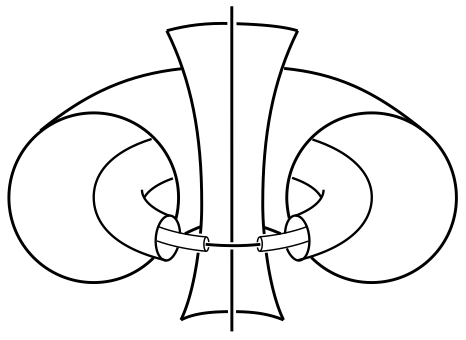
\includegraphics[width=0.5\linewidth]{hopf-bundle}
		\label{fig:hopf-bundle}
	\end{figure}
	The limiting cases $T_0$ and $T_\infty$ correspond to the unit circle in the $xy$-plane and the $z$-axis under the stereographic projection.	Each torus $T_\rho$ is aunion of circle fibers. These fiber circles have slope 1 on the torus, winding around once longitudinally and once meridionally. As $\rho$ goes to $0$ or $\infty$ the fiber circles approach the circles $T_0$ and $T_\infty$, which are also fibers. The figure below shows four tori decomposed into fibers:
	\begin{figure}[H]
		\centering
		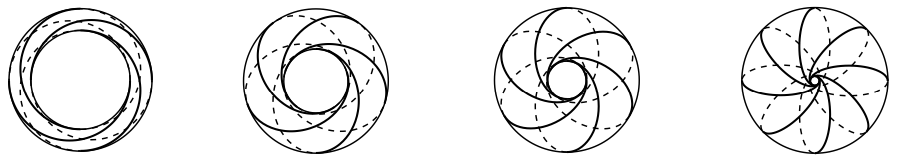
\includegraphics[width=0.9\linewidth]{hopf-bundle2}
		\label{fig:hopf-bundle2}
	\end{figure}
	
	Replacing the field $\mathbb{C}$ by the quaternions $\mathbb{H}$, the same constructions yield fiber bundles $S^3\to S^{4n+3}\to\mathbb{H} P^{n}$ over quaternionic projective spaces $\mathbb{H} P^n$. Here the fiber $S^3$ is the unit quaternions, and $S^{4n+3}$ is the unit sphere in $\mathbb{H}^{n+1}$. Taking $n=1$ gives a second Hopf bundle $S^3\to S^7\to S^4=\mathbb{H} P^1$.
	
	Another Hopf bundle $S^7\to S^{15}\to S^8$…
\end{example}

\subsection{Homotopy equivalences and weak homotopy equivalences}

\begin{defn}[Weak homotopy equivalence]
	Any map $f:X\to Y$ that induces isomorphisms on all homotopy groups ( $\forall n\geq 0$ and all choices of basepoint in $X$).
\end{defn}

\subsection*{Any Hurewicz fibration is Serre fibration}
\subsection*{Any relative CW-complex is a cofibration in Quillen model structure}
\subsection*{Any map can be replaced by…} 
\subsubsection*{an homotopy equivalence followed by Hurewicz fibration}
\subsubsection*{a Hurewicz cofibration followed by homotopy equivalence}
\subsubsection*{a Quillen cofibration followed by weak equivalence}
This one follows from CW-approximation theorem

\section*{Homotopy theory  of spaces (B)}

\subsection{Blakers-Massey theorem}

As in Hatcher and in terms of homotopy pullbacks and pushouts. (Be careful if you refer to REsk's paper for the latter version, since in his paper the $n$ in definition of $n$-connectiviy is shifted by $1$.
\begin{thm}[Blakers-Massey. Hatcher 4.23, Tom Dieck 6.4.1]
	Let $X$ be a CW complex decomposed as the union of subcomplexes $A$ and $B$ with nonempty connected intersection $C=A\cap B$ {\color{magenta}(that is also a CW complex?)}. If $(A,C)$ is $m$-connected and $(B,C)$ is $n$-connected, $m,n\geq 0$, then the map
	\[\pi_{i}(A,C)\to \pi_{i}(X,B)\]
is an isomorphism for $i<m+n$ and a surjection for $i=m+n$.
\end{thm}

\begin{prop}[Quotient theorem. Hatcher, 4.28and Tom Dieck 6.10.2]
	If a CW pair $(X,A)$ is $r$-connected and $A$ is $r,s \geq 0$, then the map $\pi_{i}(X,A)\to \pi_{n}(X/A)$ induced by the quotient map $X\to X/A$ is an isomorphism for $i\leq r+s$ and a surjection for $i=r+s+1$.
\end{prop}
\begin{proof}
	Using cones.
\end{proof}

\subsection{Freudethal suspension theorem}

\begin{coro}[Freudenthal suspension theorem, Hatcher 4.24]
	The suspension map $\pi_{i}(S^{n})\to \pi_{i+1}(S^{n+1})$ is an isomorphism for $i<2n-1$ and a surjection for $i=2n-1$. More generally, this holds for the suspension $\pi_{i}(X)\to \pi_{i+1}(SX)$ whenever $X$ is an $(n-1)$-connected CW complex.
\end{coro}
\begin{thm}[Freudenthal suspension theorem, lecture notes]
		Let $X$ be $\ell$-connected space. Then $X\to\Omega\Sigma X$ is a $(2\ell+1)$-equivalence, that is,
	\[\pi_i(X)\to \pi_{i+1}(\Sigma X),\]
	is a bijection for $i<2\ell+1$ and a surjection for $i=2\ell+1$..
\end{thm}
\begin{proof}[Proof 2 from lectures]
	Consider
	\[\begin{tikzcd}
		X\arrow[r]\arrow[d]&CX\arrow[d]\\
		CX\arrow[r]&\Sigma X
	\end{tikzcd}\]
	Then we use relative homotopy long exact sequence with $(X,CX)$ to get $\pi_i(CX,X)\cong\pi_{i-i}(X)$, which is zero for $0\leq i\leq \ell+1$. Then use relative homotopy exact sequence for the pair $(\Sigma X,CX)$. then we get that $\pi_i(\Sigma X,CX)=\pi_i(\Sigma X)$. And then if you use it for $(\Sigma X, X)$ and 
	
	But it also turns out that $\pi_i(\Sigma X)=\pi_{i-1}(\Omega\Sigma X)$ because
	\begin{align*}
		\pi_n(Z)&=\operatorname{Hom}_{\operatorname{hTop},*}(S^n,Z)=\operatorname{Hom}(S^1\wedge S^{n-1},Z)=\operatorname{Hom}(S^{n-1},\Omega Z)=\pi_{n-1}(\Omega,Z)
	\end{align*}.
	And then since $CX\hookrightarrow \Sigma X$ we get an arrow $\pi_i(CX,X)\to\pi_i(\Sigma X,CX)$ which is isomorphism for $0\leq i \leq 2\ell +1$ and surjective for $i=2\ell+2$.
	
	So apply Blakers-Massey an ell equalities to get maps fro $\pi_{i-1}(X)\to\pi_{i-1}(\Omega\Sigma X)$ for $i$ as desired.
\end{proof}
\begin{coro}
	If $X$ is $\ell$-connected, then $\Sigma X$ is $(\ell+1)$-connected for $\ell\geq0$.
\end{coro}
\[\begin{matrix}
	\text{space}&&S^0&\Sigma S^0=S^1&\Sigma^2S^0=S^2&\Sigma^3S^0=S^3&\cdots&\Sigma^nS^0=S^n\\
	\text{conectedness}&&-1&0&1&2&\cdots&(n-1)
\end{matrix}\]

\subsubsection{\texorpdfstring{$\pi_{i}(S^{n})=0$}{πᵢ(Sⁿ)} for \texorpdfstring{$i<n$}{i<n}}

\begin{coro}
	$S^n$ is $(n-1)$-connected.
\end{coro}
Back to Hopf fibration:
\[S^1\hookrightarrow S^3\to S^2\]
we get
\[0=\pi_2(S^3)\to\pi_2(S^2)\overset{\cong}{\to}\pi_1(S^1)\to\pi_1(S^3)=0,\]
so
\[\mathbb{Z}=\pi_2(S^2).\]
Now consider a map $S^n\to S^n$. We get a map $CS^n\to CS^n$ (in general, for $f:X\to Y$ we have $(t,x)\mapsto(t,f(x))$ in the cones). We also have $CS^n\to CS^n/S^n=S^{n+1}$.

Now if we take $\operatorname{id}:S^n\to S^n$ we shall get $\operatorname{id}:S^{n+1}\to S^{n+1}$. Think about this like $\pi_1(S^1)\to\pi_2(S^2)$. Now from Freudenthal we get $\pi_{i-1}(X)\to\pi_i(\Sigma X)$ is surjective because $i=0$. From Hopf fibration we have $\pi_2(S^2)=\mathbb{Z}$. So we have a surjective map $\mathbb{Z}\to\mathbb{Z}$. So it's an isomorphism and we conclude that $\operatorname{id}_{S^2}$ is a generator of $\pi_2(S^2)$.
\begin{coro}
	Since $S^n$ is $(n-1)$-connected, we have
	\[\pi_i(S^n)\to\pi_{i+1}(S^{n+1})\]
	is isomorphism for $i\leq 2(n-1)=2n-1$ and epimorphism form $i=2n-1$. (We just shift the indices of \cref{thm:freudenthal} by one.)
\end{coro}
\begin{coro}
	$\pi_n(S^n)=\mathbb{Z}$ with $\operatorname{id}_{S^n}$ as generator.
\end{coro}

\subsubsection{$\pi_{n}(S^{n})=\mathbb{Z}$}
\begin{coro}
	$\pi_{n+k}(S^n)\to\pi_{n+k+1}(S^{n+1})$ is isomorphism for $k\leq n-1$ and epimorphism for $k=n-1$.
\end{coro}
So for example
\[\pi_4(S^3)=\pi_5(S^4)=\pi_6(S^5).\]
And in fact they are $\mathbb{Z}/2$. This is what are called the \textbf{\textit{$k$th stable homotopy groups of a sphere}}. And more in general, we take any space and apply $\Omega\Sigma$ enough times, and the homotopy will start to stabilize.

Or for example from
\[S^1\hookrightarrow S^3\to S^2\]
we get
\[0=\pi_i(S^1)\to \pi_i(S^3)\overset{\cong}{\to}\pi_i(S^2)\to\pi_{i-1}(S^2)=0\]
So $\pi_3(S^2)\cong\mathbb{Z}$ in case you were wondering.
\begin{claim}[Serre]
	$\pi_{4n-1}(S^{2n})\cong\mathbb{Z}\oplus$finite abelian. And $\pi_i(S^k)$ is finite abelian in all other cases.
\end{claim}

\subsection{Whitehead theorem that weak equivalence between CW-complexes is a homotopy equivalence}

\begin{thm}[Whitehead]
	Weak homotopy equivalence for CW complexes is homotopy equivalence.

	An inclusion inducing isomorphism on all homotopy groups is a deformation retract.
\end{thm}


and related theorem that weak equivalence between bifibrant objects is a homotopy equivalence.
\subsection{Celullar approximation theorem}

\begin{defn}[Cellular map]
	A map between CW complexes $f:X\to Y$ is called \textit{\textbf{cellular}} if $f(X^{n})\subset Y^{n}$ for all $n$.
\end{defn}
\begin{thm}
	Every map between CW complex is homotopic to a cellular map.
\end{thm}
\begin{thm}[CW approximation]
	Every space has a CW approximation, ie. it is weakly equivalent to a CW-complex.	
	If $X$ is path-connected, the CW-complex can be chosen to have a single 0-cell.

	If $(X,A)$ is an $n$-connected CW-pair (so $A$ is a sub-CW-complex of $X$, made up of cells from $X$) there exists a CW-pair $(Z,A)\simeq (X,A)\operatorname{rel}A$ with cells in $Z\setminus A$ of dimension greater than $n$.
\end{thm}

\subsection*{Postnikov and Whitehead towers}

\subsubsection*{Postnikov towers}
Let $X$ be a CW complex. There exist spaces
\[\begin{tikzcd}
	&\cdots\arrow[d]\\
	&Y_{2}\arrow[d]\\
	&Y_{1}\arrow[d]\\
	X\arrow[uur]\arrow[ur]\arrow[r]&Y_{0}
\end{tikzcd}\]
that are like the original space but with trivial homotopy groups for $k\geq n$. They are obtained by attaching to the previous one {\color{blue}(or to $X$ itself?)} cells of dimension $n+2$ (because this kills the $n+1$-th homotopy group so that only the $n$-th homotopy group remains nontrivial).

The inclusions $X\hookrightarrow Y_{n}\hookrightarrow Y_{n-1}\hookrightarrow \ldots\hookrightarrow Y_{1}=K(\pi_{1}(X),1)$ are converted to fibrations, and in fact the fiber of $Y_{k}\to Y_{k-1}$ is a $K(\pi_{k}(X),k)$-space.

\subsubsection*{Whitehead towers}

Now following Laurentium Maxim, "Lecture notes on homotopy theory and applications".

\begin{defn}[\href{https://people.math.wisc.edu/~lmaxim/754notes.pdf}{754notes.pdf}]
	A \textit{\textbf{Whitehead tower}} of $X$ is a squence of fibrations
	\[\begin{tikzcd}
		\cdots \arrow[r]&X_{n}\arrow[r]&X_{n-1}\arrow[r]&\cdots \arrow[r]&X_{0}=X
	\end{tikzcd}\]
	such that
	\begin{itemize}
		\item $X_n$ is $n$-connected.
		\item $\pi_{q}(X_{n})=\pi_{q}(X)$ for $q\geq n+1$.
		\item The fiber of $X_n\to  X_{n-1}$ is a $K(\pi_{n}(X),n-1)$-space.
	\end{itemize}
\end{defn}
\begin{lemma}
	Whitehead towers exist for CW complexes.
\end{lemma}
\begin{proof}
	Consider
	\[\operatorname{hofib}\hookrightarrow X\to \text{"$X$ without $\pi_{k}$, $k>n$}"\]
	We immediately get that the second arrow induces an isomorphism on $\pi_{i}$ for $i\leq n$, while the first arrow induces isomorphisms for $i>n$. Define $ X_{n}:=\operatorname{hofib}$.

	Now notice that $X_n$ and $X_{n+1}$ have isomorphic homotopy groups except perhaps the $(n+1)$-th, because for $X_{n}$ it is already the same as that of $X$, but for $X_{n+1}$ it is still zero. So, from the fibration
	\[\operatorname{hofib} \hookrightarrow X_{n+1}\to X_{n}\]
	we get an isomorphism
	\[\begin{tikzcd}[column sep=tiny,row sep=small]
		\cdots\arrow[r]&\pi_{n+2}(X_{n})\arrow[r]\arrow[d,"\cong "]&\pi_{n+1}(\operatorname{hofib} )\arrow[d,equals]\arrow[r]&\pi_{n+1}(X_{n+1})\arrow[r]\arrow[d,equals]&\pi_{n+1}(X_{n})\arrow[r]\arrow[d,"\cong "]&\pi_{n}(\operatorname{hofib} )\arrow[r]&\pi_{n}(X_{n+1})\arrow[r]\arrow[d,equals]&\cdots\\
			       &\pi_{n+2}(X)&0&0&\pi_{n+1}(X)\arrow[ur,blue,"{\color{blue}\cong }",swap]&&0&
		\end{tikzcd}\]
	showing that the homotopy fiber of this fibration is in fact $K(\pi_{n+1}(X),n)$.
	
\end{proof}

\subsection*{How to kill higher homotopy groups without changing lower homotopy groups and lower homology}

{\color{cyan}Looks like Blakers-Massey is needed for this. The following are lecture notes corresponding to post-Blakers-Massey and pre-Postnikow towers part our the course.}

Glue a disk to a space and what happens to homotopy groups?
\[\begin{tikzcd}
	S^{n-1}\arrow[r,"(n-1)\text{-equiv}"]\arrow[d,"0\text{-equiv}",swap]&D^n\arrow[d]\\
	X\arrow[r]&X\cup D^n\arrow[ul, phantom, "\ulcorner", very near start]
\end{tikzcd}\]
Assume $X$ is connected. We get a map from the vertical arrows
\[\begin{tikzcd}
	\pi_i(D^n,S^{n-1})\arrow[r]&\pi_i(X\cup D^n,X)
\end{tikzcd}\]
which is $(n-1)$-equivalence by Blakers-Massey. So, by attaching $\sqcup D^n$ we can kill $\pi_{n-1}(X)$, that is, $X\cup(\sqcup D^n)$ has trivial $\pi_{n-1}$.

Now notice that

%since $S^{n-1}\to D^n$ is an $(n-1)$-equivalence, which is the case since
\[\begin{tikzcd}
	0=\pi_i(D^n)\arrow[r]&\pi_i(D^n,S^{n-1})\arrow[r,"\cong"]&\pi_{i-1}(S^{n-1})\arrow[r]&\pi_{i-1}(D^n)=0
\end{tikzcd}\]
that is, $\pi_i(D^n,S^{n-1})=0$ for $i\leq n-1$. This implies that $\pi_i(X\cup D^n,X)=0$ for $i\leq n-1$.

Also by homotopy long exact sequence,
\[\pi_{n-1}(X)\to \pi_i(X\cup D^n)\text{ is sujrective}\]
\[\pi_i(X)\to \pi_{i}(X\cup D^n)\text{ is isomorphism for }i\leq n-2.\]
So what we have thus far is
\[\begin{tikzcd}
	\pi_n(X\cup D^n)\arrow[r]&\pi_{n-1}(X)\arrow[r]&\pi_{n-1}(X\cup D^n)\arrow[r]&0=\pi_{n-1}(X\cup D^n)
\end{tikzcd}\]
Notice that $\pi_n(X\cup D^n,X)$ is not ingeneral cyclic (counterexample $S^1\cup D^2$ taking unieversal cover which is real line with spheres on integers, homotopy equivalent to $\bigvee_\mathbb{Z} S^2$ which is not finitely generated).

\begin{quote}
	{\color{red} So basically attaching a disk via $f$ will kill $[f]$ inside $\pi_n(X)$ this is called \textbf{\textit{killing}} an element of the homotopy group.}
\end{quote}

\begin{prop}
	For any CW-complex $X$, $X^\ell\to X$ is an $\ell$-equivalence.
\end{prop}

\begin{remark}
	We have used that for $A\hookrightarrow X$ from long exact sequence of relative homotopy groups we get $\pi_n(X,A)=0$.
\end{remark}

\begin{coro}
	Let $i\leq \ell$ and $g: D^i\to X$, $g:\partial D^i\to X^\ell$. Then there is a homotopy $\operatorname{rel}\partial D^i$ to a map with $\operatorname{img}\subset X^\ell$.
\end{coro}

\begin{thm}[Cellular approximation theorem]
	Let $X$ and $Y$ be CW-complexes and $\xi:Y\to X$ be any map. Then $\xi$ is homotopic to a \textbf{\textit{cellular map}}, that is, a map $\psi:Y\to X$, such that for all $\ell$, $\psi Y^0\subset X^\ell$.
\end{thm}

We also have
\begin{prop}
	Let $n\geq 2$. Then 
	\[\pi_n\left(\bigvee_{k\in I}S^n\right)=\bigoplus_{k\in I}\i_n(S^n)=\bigoplus_{k\in I}\mathbb{Z}=Z^{\oplus I}\]
\end{prop}
\begin{prop}
	First notice that for finite $I$,
	\[X^n=X^{n+1}=\bigvee_{k\in I}S^n\]
	by looking carefully. Then
	\[\pi_n(X,X^{n+1})=0=\pi_{n+1}(X,X^{n+1})\]
	so
	\[\bigoplus_{k\in I}\mathbb{Z}=\prod_{k\in I}\pi_n(S^n)=\pi_n(X)=\pi_n(X^{n+1})=\pi_n(X^n)=\pi_n\left(\bigvee_{k\in I}S^n\right)\]
	and for the infinite case it also works, using finite compactness of the CW complex.
\end{prop}

\section*{Homotopy theory of spaces (C)}

\subsection*{Homotopy pushouts and pullbacks}
The idea is simply to construct the homotopy version of pushouts and pullbacks. So let's remember that
\begin{defn}\leavevmode 
	\begin{itemize}
		\item A \textbf{\textit{pullback}} of the morphisms $f$ and $g$ consists of an object $P$ and two morphisms $p_1:P\to X$ and $p_2:P\to Y$ satisfying the following universal property:
		\[\begin{tikzcd}
			Q\arrow[rrd,bend left,"q_2"]\arrow[ddr,"q_1",swap,bend right]\arrow[dr,dashed,"\phi"]\\
			&P\arrow[r,"p_2"] \arrow[rd, phantom, "\lrcorner", very near start]\arrow[d,"p_1",swap]&Y\arrow[d,"g"]\\
			&X\arrow[r,"f",swap]&Z
		\end{tikzcd}\]
		\item A \textbf{\textit{pushout}} of the morphisms $f$ and $g$ consists of an object $P$ and two morphisms $i_1:P\to X$ and $i_2:P\to Y$ satisfying the following universal property:
		\[\begin{tikzcd}
			Z\arrow[r,"g"]\arrow[d,swap,"f"]&Y\arrow[d,"i_2"]\arrow[ddr,bend left,"j_2"]\\
			X\arrow[r,"i_1",swap]\arrow[drr,bend right,swap,"j_1"]&P\arrow[ul, phantom, "\ulcorner", very near start]\arrow[dr,dashed,"\phi"]\\
			&&Q
		\end{tikzcd}\]
	\end{itemize}
		\begin{remark}
			Other names for the pushout are \textbf{\textit{cofibered product of $X$ and $Y$}} (especially in algebraic categories when $i_1$ and $i_2$ are monomorphisms), or \textbf{\textit{free product of $X$ and $Y$}} with $Z$ \textbf{\textit{amalgamated sum}}, or more simply an \textbf{\textit{amalgamation}} or \textbf{\textit{amalgam of $X$ and $Y$.}}
		\end{remark}
	\end{defn}
		So basically
\begin{defn}[Homotopy pullback and homotopy pushout]
	{\color{magenta}We just ask that the diagrams above commute up to homotopy?}
\end{defn}
\begin{remark}[Concrete construction of homotopy pushout]
	We also need to ask in our definition that there is some sort of homotopy-naturality. For the case of the homotopy pushout it should look something like this:
		\[\begin{tikzcd}
			\bullet\arrow[rr]\arrow[dd]\arrow[dr]&&\bullet\arrow[d,"\simeq "]\\
			&A\arrow[r]\arrow[d]&B\arrow[d]\arrow[ddr,bend left]\\
			\bullet\arrow[r,"\simeq "]&C\arrow[r]\arrow[drr,bend right]&\bullet\arrow[ul, phantom, "\ulcorner", very near start]\arrow[dr,"\simeq" ]\\
			&&&\bullet
		\end{tikzcd}\]
	so everything is commuting up to homotopy. {\color{magenta}What are the formal definitions? Probably rather involved.} But a concrete definition of the \textit{\textbf{homotopy pushout}} according to the diagram above is
	\[B\sqcup C\sqcup A\times I\Big/\substack{A\times 0\sim B \\ A\times I\sim C}\]
\end{remark}
\begin{remark}[From lecture notes]
		The pullback of
	\[\begin{tikzcd}
		&Z^I\times_ZY\arrow[d]\\
		X\arrow[r]&Z
	\end{tikzcd}\]
	is the homotopy pullback of
	\[\begin{tikzcd}
		&Y\arrow[d]\\
		X\arrow[r]&Z
	\end{tikzcd}\]
\end{remark}
\begin{defn}[From lecture notes. {\color{magenta}Is this right?}]
	The \textbf{\textit{homotopy pullback}} of a diagram
		\[\begin{tikzcd}
			&Y\arrow[d]\\
			X\arrow[r]&Z
		\end{tikzcd}\]
		is
		\[\begin{tikzcd}
			X\times_{\operatorname{ev}_0}Z^I\times_{\operatorname{ev}_1}Y\arrow[d]\arrow[r]&Y\arrow[d]\\
			X\arrow[r]&Z
		\end{tikzcd}\]
		Intuitively, for any $x\in X$ and $y\in Y$ this object has the space of paths connecting $x$ and $y$.
\end{defn}

\subsection*{Homotopy fibers and cofibers}

Before we go, what is a fiber? Perhaps it is the same as a kernel. And a cofiber may be the same as a cokernel. Recall:
\begin{defn}[Kernel and cokernel]\leavevmode 
	\begin{itemize}
		\item The \textbf{\textit{kernel}} of a morphism is that part of its domain which is sent to zero. Formally, in a category with an initial object 0 and pullbacks, the \textbf{\textit{kernel $\operatorname{ker} f$}} of a morphism $f:A\to B$ is the pullback $\operatorname{ker}(f)\to A$ along $f$ of the unique morphism $0\to B$
		
		More explicitly, this characterizes the object $\operatorname{ker}(f)$ as \textit{the} object (unique up to isomorphism) that satisfies the following universal property:
		\begin{quote}
			for every object $C$ and every morphism $h:C\to A$ such that $f\circ h=0$ is the zero morphism, there is a unique morphism $\phi:C\to\operatorname{ker}(f)$ such that $h=p\circ\phi$.
		\end{quote}
		\[\begin{tikzcd}
			C\arrow[dr,dashed,"\phi"]\arrow[ddr,bend right,swap,"h"]\\
			&\operatorname{ker}(f)\arrow[d]\arrow[r]&0\arrow[d]\\
			&A\arrow[r,"f",swap]&B\arrow[ul, phantom, "\ulcorner", very near start]
		\end{tikzcd}\]
		\item In a category with a terminal object 1, the \textbf{\textit{cokernel}} of a morphism $f:A\to B$ is the pushout (arrows $h$ and $\phi$ apply if terminal object is zero)
		\[\operatorname{coker}(f):=1\sqcup_AB\qquad\qquad\begin{tikzcd}
			A\arrow[r,"f"]\arrow[d]\arrow[dr, phantom, "\lrcorner", very near start]&B\arrow[d]\arrow[rdd,bend left,"h"]\\
			1\arrow[r]&\operatorname{coker}(f)\arrow[dr,dashed,"\phi"]\\
			&&C
		\end{tikzcd}\]
		In the case when the terminal object is in fact zero object, one can, more explicitly, characterize the object $\operatorname{coker}(f)$ with the following universal property:
		\begin{quote}
			for every object $C$ and every morphism $h:B\to C$ such that $h\circ f=0$ is the zero morphism, there is a unique morphism $\phi:\operatorname{coker}(f)\to C$ such that $h=\phi\circ i$.
		\end{quote}
\end{itemize}
\end{defn}
{\color{magenta}The \textit{\textbf{homotopy fiber}} and the  \textit{\textbf{homotopy cofiber}} are probably just the homotopic versions of the kernel and cokernel.}

\begin{defn}[From lecture notes, {\color{magenta}looks incomplete…}]
	The \textbf{\textit{homotopy fiber}} if $f:Y\to Z$ is the pullback of
		\[\begin{tikzcd}
			&Y\arrow[d,"f"]\\
			pt\arrow[r]&Z
		\end{tikzcd}\]
		$F\subset Z^I\times_ZY\to Z$, where $F$ is the space of paths starting at $x$ and ending at the same point $f(y)$.
\end{defn}

\begin{defn}[Homotopy fiber, a concrete construction in Hatcher]
	Given a map $f:A\to B$, let $E_f$ be the space of pairs $(a,\gamma)$ where $a\in A$ and $\gamma:I\to B$ is a path in $B$ with $\gamma(0)=f(a)$. {\color{blue}So: take a point in $A$, and map it to some point in $B$, say $f(a)$. And then take any path in $B$ starting at $f (a)$.}
\begin{prop}
	The map $p:E_f\to B$ given by $p(a,\gamma)=\gamma(1)$ is a fibration.
\end{prop}
We can regard $A$ as a subspace of $E_{f}$ consisting of pairs $(a,\gamma)$ with $\gamma$ the constant path at $f(a)$, and $E_f$ deformation retracts onto this subspace by restricting all the paths $\gamma$ to shorter and shorter initial segments. The map $p:E_f\to B$ restricts to $f$ on the subspace $A$, so we have factored the map $f:A\to B$ as the composition $A\hookrightarrow E_f\to B$ of a homotopy equivalence and a fibration.

We can also think of this construction as extending $f$ to a fibration $E_f\to B$ by enlarging its domain to a homotopy equivalent space.

The fiber $F_f$ of $E_f\to B$ is called the \textit{\textbf{homotopy fiber}} of $f$. It consists of the pairs $(a,\gamma)$ with $a\in A$ and $\gamma$ a path in $B$ from $f(a)$ to a basepoint $b_0\in B$.
\end{defn}

\subsection*{Homotopy fiber of homotopy fiber}

It is interesting to see what happens when the process of forming homotopy fibers is iterated. Given a fibration $p:E\to B$ with fiber $F=p^{-1} (b_0)$, we know that the inclusion of $F$ into the homotopy fiber $F_{p}$ is a homotopy equivalence {\color{blue}(because all fibers in homotopy fibrations are homotopy equivalent?)} Well, beacause
\begin{prop}[4.66]
	If $p:E\to B$ is a fibration, then the inclusion $E\hookrightarrow E_p$ is a fiber homotopy equivalence (a fiber-preserving map of the total spaces that has an "fiber homotopy inverse" i.e. composition is homotopic to the identity via fiber-preserving maps). In particular, the homotopy fibers are homotopy equivalent to the actual fibers.
\end{prop}

Recall that the homotopy fiber $F_p$ consists of pairs $(e,\gamma)$ with $e\in E$ and $\gamma$ a path in $B$ from $p(e)$ to $b_0$. The inclusion $F\hookrightarrow E$ extends to a map $i:F_{p}\to E$, $i(e,\gamma)=e$ and \textit{this map is obviously a fibration}. In fact it is the pullback via $p$ of the path fibration $PB\to B$… {\color{blue}what could this mean? Maybe this:}
\[\begin{tikzcd}
	F_{p}\arrow[r,"i"]\arrow[d]\arrow[dr,phantom,very near start,"\lrcorner"]&E\arrow[d,"p"]\\
	PB\arrow[r]&B
\end{tikzcd}\]
Perhaps this justifies why, up to equivalence, the fiber of this map $i$ must be $\Omega B$. In the end we get the following sequence:
\[\begin{tikzcd}[column sep=small]
	\cdots\arrow[r]&\Omega^{2}B\arrow[r]&\Omega F\arrow[r]&\Omega E\arrow[r]&\Omega B\arrow[r]&F\arrow[r]&E\arrow[r]&B
\end{tikzcd}\]
where any two consecutive maps form a fibration, up to homotopy equivalence, and all the maps to the left $\Omega B$ are obtained by applying the functor $\Omega$ to the later maps. The long exact sequence of homotopy groups for any fibration in the sequence coinincides with the long exact sequence for $F\hookrightarrow E\to B$.

\subsection*{Homotopy cofiber of homotopy cofiber}

The dual construction to the sequence above is
\[\begin{tikzcd}[column sep=small]
	X\arrow[r]&Y\arrow[r]&M_{f}\arrow[r]&\Sigma X\arrow[r]&\Sigma Y\arrow[r]&\Sigma M_{f}\arrow[r]&\Sigma^{2}X\arrow[r]&\cdots 
\end{tikzcd}\]

\subsection*{The two Dold-Puppe sequences, their (co)-exactness}

\subsection*{Fiber of a (Serre) Hurewicz fibration is a (weak) homotopy fiber}

\subsection*{Fiber bundles are Serre fibrations}
We've been talking a lot about Hurewicz fibrations. Let's talk about Serre fibrations. Notice that H. fibration $\implies$ S. fibration. What is the most natural example of a Serre fibration?

\begin{prop}[Hatcher, 4.48]
	Let $E$ be a fiber bundle with fiber $F$. Then $f$ is a Serre fibration.
\end{prop}
\begin{proof}
	What sdoes it mean to be a Serre fibration? It means that
	\[\begin{tikzcd}
		I^n\arrow[r]\arrow[d]&E\arrow[d]\\
		I^{n+1}=I^n\times I\arrow[r]\arrow[ur,dashed]&B
	\end{tikzcd}\]
	So if $\mathcal{U}$ is a covering of $B$ such that $f^{-1}U\cong U\times F$. By Lebesgue lemma, there is a $\delta>0$ such that for all $x\in I^{n+1}$, the ball $B(x,\delta)$ lies in some $f^{-1}U$ for some $U$.
	
	Then we subdivide $I^{n+1}$ in smaller cubes of the same size with diameter $<\delta$. So, each the image of each cube lies in some $U\in\mathcal{U}$.
	
	Then
	\[\begin{tikzcd}
		I^n\arrow[d]\arrow[r]&F\times U\arrow[d,two heads]\\
		I^{n+1}\arrow[r]\arrow[ur,dashed]&U
	\end{tikzcd}\]
	has a lift for every little square because
	\[\begin{tikzcd}
		X\arrow[r]\arrow[d]&U\arrow[d]\\
		X\times I\arrow[r]\arrow[ur,dashed]&pt
	\end{tikzcd}\]
	is always a fibration {\color{orange}(think about this)} and because pullbacks of fibrations are fibrations:
	\[\begin{tikzcd}
		U\times F\arrow[r,two heads]\arrow[d,two heads]&U\arrow[d,two heads]&\\
		F\arrow[r,two heads]&pt
	\end{tikzcd}\].
	Then we may just add up the squares because
	\[\begin{tikzcd}
		D^n\arrow[d]\\
		D^n\times I
	\end{tikzcd}\]
	and we're done.
\end{proof}

\subsection{Long exact sequence of homotopy groups associated to Serre fibration}
\begin{thm}[Hatcher 4.41]
	Suppose $p:E\to B$ is a Serre fibration. Choose basepoints $b_{0}\in B$ and $x_{0}\in F=p^{-1}(b_{0})$. Then the map $p_{*}:\pi_{n}(E,F,x_{0})\to \pi_{n}(B,b_{0})$ is an isomorphism for all $n\geq 1$.

	Hence, if $B$ is path connected, there is a long exact sequence
\[\begin{tikzcd}
	\cdots\arrow[r]&\pi_n(F)\arrow[r]&\pi_n(E)\arrow[r]&\pi_n(B)\arrow[r]&\pi_{n-1}(F)\arrow[r]&\pi_{n-1}(E)\arrow[r]&\cdots\\
	\cdots\arrow[r]&\pi_n(F)\arrow[r]\arrow[u,equals]&\pi_n(E)\arrow[r]\arrow[u,equals]&\pi_n(E,F)\arrow[r]\arrow[u,"\cong "]\arrow[u,swap,"p_{*}"]&\pi_{n-1}(F)\arrow[r]\arrow[u,equals]&\pi_{n-1}(E)\arrow[r]\arrow[u,equals]&\cdots
\end{tikzcd}\]
\end{thm}

\subsection*{Fiber bundles over manifolds are Hurewicz fibrations}

\section*{Homotopy theory of spaces (D)}

\subsection{Eilenberg-MacLane spaces}
A space $X$ having jut one nontrivial homotopy group $\pi_{n}(X)\cong G$ is called an \textit{\textbf{Eilenberg-MacLane space}} $K(G,n)$. We can build a CW complex $K(G,n)$ by the familiar construction of attaching cells to a wedge of spheres, acounting for generators and relations, and then attaching further cells to kill higher homotopy groups.

\begin{prop}[4.30]
	The homotopy type of a CW complex $K(G,n)$ is uniquely determined by $G$ and $n$.
\end{prop}
\begin{proof}[Idea of proof]
	Attaching cells and Whithead theorem.
\end{proof}

\subsection{Representable functors and Yoneda lemma}

\begin{defn}[Representable functor]
	Let $\mathcal{C}$ be a category. A functor $F:\mathcal{C}^{\operatorname{op}}\to \operatorname{Sets}$ is called \textit{\textbf{representable}} if there exists an object $B=B_{F}$ in $\mathcal{C}$ with the property that there is a \textit{natural} isomorphism of functors
	\[\varphi:\mathcal{C}(-,B_{F})\to F\]
	where $\mathcal{C}(-,B_{F})$ is the set of arrows from $-$ to $B_{F}$.

	One ussually expresses the naturality condition for a map $f:X\to Y$ with the following diagram:

	\[\begin{tikzcd}
		\mathcal{C}(X,B)\arrow[r,"\varphi_{X}"]\arrow[d,"f^{*}"]&F(X)\arrow[d,"f^{*}"]\\
		\mathcal{C}(Y,B)\arrow[r,"\varphi_{Y}"]&F(Y)
	\end{tikzcd}\]
\end{defn}

\begin{remark}
	By applying $\varphi_{B}$ to the identity map  $B\to B$ we obtain a special element $\gamma=\varphi_{B}(\operatorname{id})\in F(B)$, which is \textit{generic} in the sense that any element $\xi \in F(X)$ can be obtained as $\xi=f^{*} (\gamma)$, for a suitable $f:X\to B$. Indeed, one can take $f=\varphi^{-1}_{X}(\xi)$ and apply naturality to check that $\xi=f^{*}(\gamma)$. 
\end{remark}


\begin{lemma}[Yoneda, \href{https://en.wikipedia.org/wiki/Yoneda_lemma}{wiki}]
	Let $F$ be a functor from a locally small category $\mathbb{C}c$ to $\operatorname{Set}$. Then for each object $X$ of $\mathbb{C}c$, the natural transformations $\operatorname{Nat}(\operatorname{Hom}(X,-),F)$ are in one-to-one correspondence with the elements of $F(X)$, that is
	\[\operatorname{Nat}(\operatorname{Hom}(X,-), F)\cong F(X)\]
	Moreover, this isomorphism is natural in $A$ and $F$ when both sides are regarded as functors from $\mathbb{C}c\times\operatorname{Set}^{\mathbb{C}c}$ to $\operatorname{Set}$. ($\operatorname{Set}^{\mathbb{C}c}$ denotes de category of functors from $\mathbb{C}c$ to $\operatorname{Set}$.)
	
	There is a contravariant version of Yoneda lemma asserting that if $F$ is a contravariant functor from $\mathbb{C}c$ to $\operatorname{Set}$,
	\[\operatorname{Nat}(\operatorname{Hom}(-,X), F)\cong F(X).\]
\end{lemma}
\begin{coro}
	$\operatorname{Nat} (\operatorname{Hom}(-,X),\operatorname{Hom}(-,Y))\cong\operatorname{Hom}(X,Y)$.
\end{coro}
\begin{remark}
	The correspondence $X\mapsto\operatorname{Hom}(-,X)$ is fully faithful, that is, the correspondence $\operatorname{Hom}(X,X')\to\operatorname{Nat}(\operatorname{Hom}(-,X),\operatorname{Hom}(-,X'))$ is injective and bijective.
\end{remark}

\subsection{Brown's representability theorem}

\subsubsection{In lecture13.pdf}

See \href{https://www.math.ru.nl/~gutierrez/files/Lecture13.pdf}{Lecture 13: Representable functors and the Brown Representability Theorem.pdf}

Let us summarize the discussion so fat. Suppose that
\[F:\operatorname{Ho}(\operatorname{Top}_*)^{\operatorname{op}}\to \operatorname{Sets}_{*}\]
is a functor having the following two properties:
\begin{enumerate}[label=(\roman*)]
	\item $F\left( \bigvee_{i\in I}X_{i} \right) \to \prod_{i\in I}F(X_{i})$ is an isomorphism for any family of pointed spaces $\{X_{i}\} $.
\item {\color{blue}"Pushout where one of the arrows is a cofibration goes to weak pullback".} $F(B\cup_{A}C)\to F(B)\times_{F(A)} F(C)$ is a surjection for any two cofibrations $A\to B$ and $A\to C$.
\end{enumerate}

Then we also have
\begin{enumerate}[label=(\roman*)]\setcounter{enumi}{2}
	\item $F(*)=*$
	\item If we have a pushout of pointed spaces
		\[\begin{tikzcd}
			A\arrow[r]\arrow[d]&X\arrow[d]\\
			B\arrow[r]&Y
		\end{tikzcd}\]
		in which $i$ is a cofibration, then  $F(Y)\to F(B)\times_{F(A)}F(X)$ is a sujrection.
	\item If $\begin{tikzcd}A\arrow[r,shift={(0,0.07)}]\arrow[r,shift={(0,-0.07)}]&B\arrow[r]&C\end{tikzcd}$ is a coequalizer of pointed spaces in which the two maps form a cofibration $A\vee A\to B$, then $F(C)\to F(B)$ maps surjectively to the equalizer of $\begin{tikzcd}F(B)\arrow[r,shift={(0,0.07)}]\arrow[r,shift={(0,-0.07)}]&F(A)\end{tikzcd}$.
	\item If $X_{0}\to X_{1}\to X_{2}\to \ldots$ is a sequence of cofibrations, then $F(X)\to \lim_{\leftarrow}$ is a sujection.
\end{enumerate}

\begin{thm}[Brown representability theorem]
	Let $F$ be a contravariant functor from the homotopy category of parallel connected CW-complexes to pointed sets. If $F$ satisfies conditions (i) and (ii) above (for any pointed connected CW-complexes $X_{i}$, $A$, $B$, $C$), then $F$ is representable.
\end{thm}

\begin{remark}[So what is a classifying space?]
	The theorem says that there is a space $B=B_{F}$ (itself a pointed CW-complex) for which there is a natural isomorphism
	\[\varphi :[X,B_{F}]_{*}\overset{\cong }{\longrightarrow}F(X)\]
	for any pointed CW-complex $X$. This space $B_{F}$ is called a \textit{\textbf{classifying space}} for $F$. Recall also that when such $\varphi$ exists, it is completely determined by a \textit{generic} element $\gamma\in F(B_{F})$.

	The classifying space together with the genereic element is unique up to homotopy.
\end{remark}

Now let's sketch how the proof of Brown representability theorem goes.

\begin{defn}
	$(B,\gamma)$ is a \textit{\textbf{spherical classifying space}} for $F$ if $\gamma\in F(B)$ is an element inducing an isomorphism
	\[\gamma_{*}:[S^{n},B]_{*}\to F(S^{n}),\qquad \gamma_{*}(f)=f^{*} (\gamma)\]
	for any sphere $S^{n}$, $n>0$.
\end{defn}

\begin{remark}
	If $(B_{1},\gamma_{1})$ and $(B_{2},\gamma_{2})$ are two such spherical classifying spaces in the category $\mathcal{C}$, and $f:B_{1}\to B_{2}$ is a map with $f^{*} (\gamma_{2})=\gamma_{1}$, then $f$ induces isomorphisms
	\[\pi_{n}(B_{1})\to \pi_{n}(B_{2})\]
	between the homotopy groups for each $n>0$.

	Since $B_{1}$ and $B_{2}$ are pointed connected CW-complexes, this means that $f$ is a weak homotopy equivalence, hence a homotopy equivalence by Whitehead theorem.
\end{remark}

The proof of Brown representability theorem is based in the following two lemmas:

\begin{lemma}
	Let $X$ be a pointed CW-complex and let $\xi \in F(X)$. Then there exists a spherical classifying space $(B,\gamma)$ for $F$ with a cofibration  $f:X\to B$ with $f^{*} (\gamma)=\xi$.
\end{lemma}

And in fact,

\begin{lemma}
	Any spherical classifying space $(B,\gamma)$ for $F$ is a classifying space.

	(Thus, $\gamma_{*}:[X,B]_{*}\to F(X)$ is an isomorphism for any pointed connected CW-complex $X$, not just for spheres.
\end{lemma}

\subsubsection*{In Hatcher}

\begin{thm}[4.57]
	There are natural bijections $T:\left<X,K(G,n) \right> \to H^{n}(X;G)$ for all CW complexes $X$ and all $n>0$, with $G$ any abelian group. Such a $T$ has the form $T([f])=f^{*}$ for a certain distinguised class $\alpha\in H^{n}(K(G,n);G)$.
\end{thm}

\begin{defn}[Fundamental class]
	A class $\alpha\in H^{n}(K(G,n);G)$ with the property stated in the theorem is called a \textit{\textbf{fundamental class}}.
\end{defn}


\begin{thm}[4E.1]
	Every reduced cohomology theory on the category of basepointed CW complexes and basepoint-preserving maps has the form $h^{n} (X)=\left<X,K_{n} \right> $ for some $\Omega$-spectrum $\{K_{n}\} $.
\end{thm}


\subsection*{Representability of generalized cohomology theories}

\subsection{$H^{n}(-,G)$ is represented by  $K(G,n)$ together with a chosen element in $H^{n}(K(G,n),G)$}

Reduced cohomology is representable since

\begin{enumerate}[label=(\roman*)]
	\item $\widetilde{H}^{n}(\bigvee_{i}X_{i})=\prod_{i} \widetilde{H}_{n}(X_{i})$.
	\item Also holds. 
\end{enumerate}

What is the classifying space? Well, we have
\[[S^{p},B]=H^{n}(S^{p})=\begin{cases}
	0\qquad &p\neq n\\
	\mathbb{Z}\qquad &p=n
\end{cases}\]
which means that $B\cong K(\mathbb{Z},n)$. More explicityly, we see that the homotopy groups of the classifying space must coincide with the reduced cohomology groups, which are zero in all but the $n$-th dimension.

\subsection*{Eilenberg-MacLane spaces can be construced from Moore spaces by killing higher homotopy groups}
\subsection*{Definition of $\Omega$-spectrum}


\subsection{Hurewicz homomorphism}
\begin{defn}[Hurewicz homomorphism]
	\begin{align*}
		h: \pi_{n}(X) &\longrightarrow H_{n}(X) \\
		[f] &\longmapsto f_{*}(\alpha)
	.\end{align*}
\end{defn}
where $\alpha$ is a generator of $ H_{n}(S^{n})$.

\subsection{Absolute and relative versions of Hurewicz theorem}
\begin{thm}[Hurewicz]
	If $X$ is $n$-connected for some $n\geq 2$, then $\tilde{H}_{i}(X)=0$ for $i<n$ and $\pi_{n}(X)\cong H_{n}(X)$.
\end{thm}
\begin{coro}
	If $X$ and $Y$ are simply connected CW-spaces and $f:X\to Y$ induces isomorphisms $H_{n}(X)\cong H_{n}(Y)$ for all $n$, then it is an homotopy equivalence.
\end{coro}
\begin{thm}[Relative Hurewicz]
	If $(X,A)$ is $(n-1)$-connected, so $\pi_{n}(X,A)=0$ for $i\leq n-1$, for some $n\geq 2$ and $A$ is simply connected, then $H_{i}(X,A)=0$ for $i\leq n-1$ and $\pi_{n}(X,A)\cong H_{n}(X,A)$.

	\textit{Note. Perhaps $X$ should be $(n-1)$-connected for the relative version too---they are stated together in Hatcher.}
\end{thm}
\begin{thm}[Relative Hurewicz for general $A$]
	If $(X,A)$ is an $(n-1)$-connected pair of path-connected spaces with $n\geq 2$ and $A\neq \varnothing $, then  $h':\pi_{n}'(X,A,x_{0})\to H_{n}(X,A)$ is an isomorphism and $H_{i}(X,A)=0$ for $i<n$.
\end{thm}



\section{Spectral sequences}

\subsection{Exact couple. Spectral sequence of an exact couple.}

These notes are based on S. Burkin lecture notes and Hatcher.

\begin{enumerate}
	\item Suppose a space $X$ is expressed a union of a sequence of subspaces
		\[\ldots\subset X_p\subset X_{p+1}\subset \ldots X.\]
		Such a sequence is called a \textit{\textbf{filtration of $X$}}. For example, $X$ could be a CW complex and $X_p$ its $p$-skeleton.

	\item Given such a filtration, for every $p$ we have a pair $(X_p,X_{p-1})$ that yields a long exact sequence. All these long exact sequences can be arranged in a staricase fashion:
\[\begin{tikzcd}[column sep=tiny,row sep=small]
	H_{p+q}(X_p)\arrow[r]\arrow[d,"i",swap]\arrow[r,red,shift={(0,0.2)}]&H_{p+q}(X_p/X_{p-1})\arrow[r]\arrow[r,red,shift={(0,0.2)}]\arrow[d]&H_{p+q-1}(X_{p-1})\arrow[r]\arrow[d,red,shift={(0.2,0)}]\arrow[d,"i",swap]&H_{p+q-1}(X_{p-1}/X_{p-2})\arrow[d]\arrow[r]&\cdots\\
	H_{p+q}(X_{p+1})\arrow[r]\arrow[d,"i",swap]&H_{p+q}(X_{p+1}/X_{p})\arrow[r]\arrow[d]&H_{p+q-1}(X_{p})\arrow[r,"j",swap]\arrow[r,red,shift={(0,0.2)}]\arrow[d,"i",swap]&H_{p+q-1}(X_{p}/X_{p-1})\arrow[r,red,shift={(0,0.2)}]\arrow[d]\arrow[r,"k",swap]&\cdots\\
	\cdots&\cdots&\cdots&\cdots
\end{tikzcd}\]
	\item If you put all the absolute groups $H_n(X_p)$ in a big $A=\bigoplus_{n,p\in \mathbb{N}}H_n(X_p)$ and all the relative $H_n(X_p,X_{p-1})$ in a big $E=\bigoplus_{n,p\in \mathbb{N}}H_n(X_p,X_{p-1})$, you can write all those long exact sequences in a compact triangle diagram called an \textit{\textbf{exact couple}} triangle diagram
	\[
	\begin{tikzcd}
		A\arrow[rr,"i"]&&A\arrow[dl,"j"]\\
		&E\arrow[ul,"k"]
	\end{tikzcd}
\]
here the maps $i,j$ and $k$ are just the maps from the long exact sequences in the other big diagram (which makes the exact couple actually \textit{exact}).

	\item There is a nice way to define new groups $A'$ and $E'$ and maps between them that yield a \textit{\textbf{derived couple}}, which is another exact couple.	Namely,
		\begin{itemize}
			\item $A^1_{n,p}:=H_n(X_p)$
			\item $E^1_{n,p}:=H_n(X_p,X_{p-1})$.
			\item $d:=jk$
			\item $E':=\operatorname{ker} d/\operatorname{img}d$, the homology of $E$ respect to $d$.
			\item $A':=i(A)\subset A$.
			\item $i':=i|_{A'}$.
			\item $j'(ia):=[ja]\in E'$.
			\item $k'[e]:=ke$.
		\end{itemize}
	anyway, they are well defined and yield the exact
	\[\begin{tikzcd}[column sep=small,row sep=small]
		A'\arrow[rr,"i'"]&&A'\arrow[dl,"j'"]\\
		&E'\arrow[ul,"k'"]
	\end{tikzcd}\]

	\item The sequence $E,E',\ldots$ is called a \textit{\textbf{spectral sequence}}.
\end{enumerate}

\subsection*{First quadrant. Convergence}

[Explanation that when the spectral sequence is defined only in the first quadrant it eventually stabilizes and $E_{\infty}$-page is well-defined.]

\subsection*{Filtration on an \texorpdfstring{$R$}{R}-module and its associated graded}

\subsection*{Homological and cohomological spectral sequences}

[Subsection missing]

\begin{remark}
	The differentials in the spectral sequence for homology go up-left and for cohomology they go right-down.
\end{remark}

\subsection*{Serre spectral sequence}

\subsubsection{Homological version}

\begin{thm}[Serre spectral sequence for homology]
	Let $F\to X\to B$ be a fibration with $B$ path-connected. If $\pi_1(B)$ acts trivially on $H_*(F;G)$, then there is a spectral sequence $\{E^r_{p,q},d_r\}$ with
	\begin{itemize}
		\item
			\[d^r_{p,q}:E^r_{p,q}\to E^r_{p-r,q+r-1}\qquad \text{and} \qquad E^{r+1}_{p,q}=\operatorname{ker} d^r_{p,q}/\operatorname{img} d^r_{{\color{magenta}?}}\]
		\item The groups
			\[F_pH_n:=\operatorname{img}(H_n(X_p)\to H_n(X))\]
		where the map $H_{n}(X_p)\to H_{n}(X)$ is just the induced map by inclusion $X_p\hookrightarrow X$, form a filtration
			%\item Stable terms $E^\infty_{p,n-p}$ are isomorphic to the successive quotients $F_n^p/F^{p-1}_n$ in a filtration
		\[0\subset F_0H_n\subset \ldots\subset F_nH_n=H_n(X;G)\]
		of $H_n(X;G)$ such that
		\[E^\infty_{p,n-p}\cong F_pH_n/F_{p-1}H_n.\]
		Another way to write this is
		\[E_{p,q}^\infty=F_pH_{p+q}\Big/F_{p-1}H_{p+q}.\]
	\item \[E^2_{p,q}\cong H_p(B;H_q(F;G))\]
\end{itemize}
\end{thm}

\begin{remark}
	In the case of a Serre fibration, for $p\gg n$ the map $H_{n}(X_p)\to H_{n}(X)$ is an isomorphism. The group $\bigoplus_{p}F^p_n/F^{p-1}_n$ is called the \textit{\textbf{associated graded group of the filtered group $H_n(X)$}}.
\end{remark}

\begin{remark}[Quote from Hatcher]
	If the coefficient group $G$ is a field then $H_{n}(X;G)$ is the direct sum $\bigoplus_{p} E^\infty_{p,n-p}$.
\end{remark}

\begin{question}
	Can we recover $H^{n}(E)$ in general? No.
\end{question}

\subsubsection{Cohomological version}

\begin{thm}[Serre spectral sequence for cohomology]
	Let $F\to X\to B$ be a Serre fibration with $\pi_0(B)=0$ such that the action $\pi_1(B)\curvearrowright H^*(F;G)$ is trivial.

	Then there is a spectral sequence $\{E_r^{p,q},d_r\}$ such that
\begin{itemize}
	\item \[d_r:E_r^{p,q}\to E_r^{p+r,q-r+1}\qquad\text{and} \qquad  E_{r+1}^{p,q}=\operatorname{ker} d_r/\operatorname{img} d_r.\]
	\item The groups
		\[F^pH^n:=\operatorname{img} (F^pH^n\to F^nH^n=H^n(X))\]
	form a filtration
	\[H^{n}(X)=F^0H^n\supset F^1H^n\supset \ldots\supset F^nH^n\supset \varnothing \]

	of $H^{n}(X,G)$ such that
	\[E_{\infty}^{p,q}\cong F^pH^{p+q}/F^{p+1}H^{p+q}.\]
\item \[E^{p,q}_2\cong H^p(B,H^{q}(F,G)).\]
\end{itemize}
\end{thm}

\subsection{Product in cohomological Serre spectral sequence}
Hatcher, Spectral sequences p. 543.

The Serre spectral sequence for cohomology becomes much more powerful when cup products are brought into the picture. For this we need to consider cohomology with coefficients in a ring $R$ rather than just a group $G$. What we will show is that the spectral sequence can be provided with bilinear products
\[E^{p,q}_{r}\times E^{s,t}_{r}\to E^{p+s,q+t}_{r}\]
for $1\leq r\leq \infty$ satisfying the following properties
\begin{itemize}
	\item Each differential $d_{r}$ is a derivation, satisfying
		\[d(xy)=(dx)y+(-1)^{p+q} x(dy)\qquad \forall x\in E^{p,q}_{r}\]
	This implies that the product on page $r$ induces a product in page $r+1$, and the product in page $\infty$ shall be the one induced by previous products.
	\item The product on the second page, $E^{p,q}_{2}\times E^{s,t}_{2}\to E^{p+s,q+t}_{2}$ is $(-1)^{qs}$ times the standard {\color{magenta}(standard? because as I remember cup product did not move the coeffients, right?)} cup product
		\[H^{p}(B;H^{q}(F;R))\times H^{s}(B;H^{t}(F;R))\to H^{p+s}(B;H^{q+t}(F;R))\]
		sending a pair of cocycles $(\phi,\psi)$ to $\phi\smile \psi$ {\color{magenta}where coefficients are multiplied via the cup product $H^{q}(F;R)\times H^{t}(F;E)\to H^{q+t}(F;R)$}.
	\item The cup product in $H^{*}(X;R)$ restricts to maps $F^{m}_{p}\times F^{n}_{s}\to F^{m+n}_{p+s}$. These induce quotient maps $F^{ m}/F^{m}_{p+1}\times F^{n}_s/F^{n}_{p+s}\to F^{m+n}_{p+s}/F^{m+n}_{p+s+1}$ that coincide with the product $E^{p,m-p}_{\infty}\times E^{s,n-s}_{\infty}\to E^{p+s,m+n-p-s}_{\infty}$.
\end{itemize}

\subsection{Wang spectral sequence}

Let's use lecture notes and \href{https://en.wikipedia.org/wiki/Spectral_sequence#Wang_sequence}{wikipedia} to understand Wang spectral sequence.

Consider a fibration over a sphere $F\hookrightarrow E\to B$. According to our theorem for Serre spectral sequences, we know that the $n$-th page looks as follows:
\begin{align*}
\begin{array}{c|cccccccc}
	n&H_n(F)&&&&&&&H_{n}(F)\\
	 &\vdots&&&&&&&\vdots\\
	2&H_2(F)&&&&&&&H_2(F)\\
	1&H_1(F)&&&&&&&H_1(F)\\
	0&H_0(F)&&&&&&&H_0(F)\\
	\hline\\
	 &0&&&\ldots&&&&n
\end{array}
\end{align*}

We can see there can be nontrivial differentials only on the $n$th page, so that $E^{n+1}=E^n$. Moreover, the differentials that don't vanish is are of the form
\[\begin{tikzcd}
E^n_{n,q}\arrow[r,"d^n_{n,q}"]&E^n_{0,q+n-1}
\end{tikzcd}\]

For $d_{n,q-n}^n$ we obtain
\[\begin{tikzcd}
	0\arrow[r]&\operatorname{ker} d^n_{n,q-n}\arrow[r,"\text{inclusion} ",hook]&E^n_{n,q-n}\arrow[r,"d^n_{n,q-n}"]&E^n_{0,q-1}\arrow[r,"\text{quotient}",two heads]&\operatorname{coker}d^n_{n,q-n}\arrow[r]&0
\end{tikzcd}\]
But all that is just
\[\begin{tikzcd}[row sep=small]
	0\arrow[r]&\operatorname{ker} d^n_{n,q-n}\arrow[r,"\text{inclusion} ",hook]\arrow[d,equals]&E^n_{n,q-n}\arrow[r,"d^n_{n,q-n}"]\arrow[d,equals]&E^n_{0,q-1}\arrow[r,"\text{quotient}",two heads]\arrow[d,equals]&\operatorname{coker}d^n_{q-n}\arrow[r]\arrow[d,equals]&0\\
	0\arrow[r]&\dfrac{\operatorname{ker} d^n_{n,q-n}}{\cancelto{0}{\operatorname{img} d^{n-1}_{n,q-n}}}\arrow[r]\arrow[d,equals]&E^2_{n,q-n}\arrow[r]\arrow[d,equals]&E^2_{0,q-1}\arrow[r]\arrow[d,equals]&\dfrac{E^n_{n,q-n}}{\operatorname{img} d^n_{n,q-n}} \arrow[d,equals]\arrow[r]&0\\
	0\arrow[r]&E^\infty_{n,q-n}\arrow[r]&H_{q-n}(F)\arrow[r]&H_{q-1}(F)\arrow[r]&E^{\infty}_{0,q-1}\arrow[r]&0
\end{tikzcd}\]
This is the first "half" of the Wang sequence. For the other half recall that by the theorem of Serre spectral sequence for homology we know that
\[E^{\infty}_{p,n-p}=F_pH_n/F_{p-1}H_n\]
for a filtration on the $n$-th homology group of the total space 
\[\varnothing=F_{-1}\subset F_0 \subset F_1\subset \ldots\subset F_n=H_{n}(E).\]
And recall that we may also write
\[E^\infty_{p,q}=F_pH_{p+q}/F_{p-1}H_{p+q}.\]
Then we can see that
\[\begin{tikzcd}[row sep=small]
	0\arrow[r]&E^\infty_{0,q}\arrow[d,equal]\arrow[r,"i^*"]&H_{q}(E)\arrow[r]&E^\infty_{n,q-n}\arrow[r]\arrow[d,equal]&0\\
		  &\dfrac{F_0H_{q}(F)}{\cancelto{0}{F_{-1}H_{q}(F)}} &&\dfrac{F_nH_{q}(E)}{F_{n-1}H_{q}(E)}
\end{tikzcd}\]
But 
\[E^\infty_{0,q}=\dfrac{F_0H_{q}(F)}{\cancelto{0}{F_{-1}H_{q}(F)}}{\color{magenta}\quad \overset{\text{why?}}{=}}H_{q}(F)\]

This is the other "half" of the Wang sequence. It only remains to put both halves together and conclude that
\[\begin{tikzcd}[column sep=small]
	\cdots\arrow[r]&H_{q}(F)\arrow[r,"i^*"]&H_{q}(E)\arrow[r]&E^{\infty}_{n,q-n}\arrow[r,"d^n_{n,q-n}"]&H_{q-n}(F)\arrow[r]&H_{q-1}(F)\arrow[r]&E^\infty_{0,q-1}\arrow[r]&\cdots
\end{tikzcd}\]
But we may remove the $E^\infty$ terms to get
\[\begin{tikzcd}[column sep=small]
	\cdots\arrow[r]&H_{q}(F)\arrow[r,"i^*"]&H_{q}(E)\arrow[r]&H_{q-n}(F)\arrow[r,"d^n_{n,q-n}"]&H_{q-1}(F)\arrow[r]&H_{q-1}(E)\arrow[r]&H_{q-n-1}(F)\arrow[r]&\cdots
\end{tikzcd}\]

\subsection{Extra: spectral sequences for chain complexes and the Fr\"olicher spectral sequence}
Let's follow Griffiths and Harris to construct a nice generalization of this theory.

A \textit{\textbf{chain complex}} $(K^\bullet,d)$ is a sequence of abelian groups (if working in the category $\operatorname{ab}$)
\[\begin{tikzcd}[column sep=small]
	K^{0}\arrow[r,"d"]&K^{1}\arrow[r,"d"]&K^2\arrow[r,"d"]&\cdots
\end{tikzcd}\]
such that the differential $d$ satisfies $d\circ d=0$. We have \textit{\textbf{cohomology groups}} 
\[H^{p}(K^*)=\frac{\operatorname{ker} d:K^p\to K^{p+1}}{\operatorname{img} d:K^{p-1}\to K^p}\]
and the \textit{\textbf{cohomology ring}}
\[H^{*}(K^*)=\bigoplus_{p\geq 0} H^{p}(K^*).\]

A \textit{\textbf{subcomplex}} $(J^*,d)$ is given by subgroups $J^*\subset K^*$. with $dJ^*\subset J^*$. The \textit{\textbf{quotient complex}} $(L^*,d)$ is also well-defined by $L^*=K^*/J^*$ and the obvious differential. this construction yields a \textit{\textbf{short exact sequence of complexes}}
\[\begin{tikzcd}
	0\arrow[r]&J^*\arrow[r]&K^*\arrow[r]&L^*\arrow[r]&0
\end{tikzcd}\]
and by the fundamental theorem of homological algebra, this yields
\[\begin{tikzcd}
	\cdots\arrow[r]&H^{p}(J^*)\arrow[r]&H^{p}(K^*)\arrow[r]&H^{p}(K^*)\arrow[r]&H^{p+1}(J^*)\arrow[r]&\cdots
\end{tikzcd}\]

Generalizing the notion of subcomplex, a \textit{\textbf{filtered complex}} $(F^pK^*,d)$ is a decreasing sequence of subcomplexes
\[K^*=F^0K^*\supset F^1K^*\supset\cdots\supset F^nK^*\supset F^{n+1}K^*=\{0\}\]
and the spectral sequence will generalize the long exact sequence in cohomology.

The \textit{\textbf{associated graded complex}} to a filtered complex $ (F^pK^*)$ is the complex
\[\operatorname{Gr}K^*=\bigoplus_{p>0} F^pK^*/F^{p+1}K^* \]
with the obvious differential. The filtration $F^pK^*$ on $K^*$ also induces a filtration $F^pH^*(K^*)$ on cohomology by {\color{blue}(I think)}
\[F^pH^q(K^*)=\frac{\operatorname{ker} d:F^pK^q\to F^pK^{q+1}}{\operatorname{img} d:F^pK^{q-1}\to F^pK^q}\]
This means that the $F^pH^q(K^*)$ are subgroups of $H^{q}(K^*)$. This filtration in turn induces an \textit{\textbf{associated graded in cohomology}}
\[\operatorname{Gr}H^*(K^*)=\bigoplus_{p,q}F^pH^q(K^*)\big/F^{p+1}H^q(K^*)  \]

\begin{defn}
	A \textit{\textbf{spectral sequence}} is a sequence $\{E_r,d_r\}$ with $r\geq 0$ of bigraded groups
	\[E_r=\bigoplus_{p,q\geq 0} E^{p,q}_r \]
together with differentials
\[d_r:E^{p,q}_r\to E^{p+r,q-r+1}_r,\qquad d^2_r=0\]
such that
\[{\color{magenta}H^{*}(E_r)=E_{r+1}}\]
{\color{magenta}I just wonder what is the cohomology of a bigraded group, right? there are several chain complexes and cohomologies, but ok…}
\end{defn}

\begin{prop}[existence and description of the chain complex spectral sequence]
	Let $K^*$ be a filtered complex. then there exists a spectral sequence $\{E_r\}$ with
	\begin{align*}
		E^{p,q}_0&=F^pK^{p+q}/F^{p+1}K^{p+q},\\
		E^{p,q}_1&=H^{p+q}\left( F^pK^*/F^{p+1}K^* \right)\\
		E^{p,q}_\infty&=F^pH^{p+q}(K^*)\big/F^{p+1}H^{p+q}(K^*)
	\end{align*}
and we just say that the spectral sequence \textit{\textbf{abuts}} to $H^{*}(K^*)$.
\end{prop}

\paragraph{Explanation.} We have defined four objects:
\begin{enumerate}
	\item A filtered complex.
	\item A graded complex associated to the filtered complex whose entries are direct sums of quotients of the filtered complex.
	\item A filtration on the cohomology of the complex given by the cohomologies of every complex of the filtered complex.
	\item A graded complex associated to the filtration on the cohomology whose entries are direct sums running over the cohomology groups and the filtration entries.
\end{enumerate}
And the proposition says is that there is a spectral sequence such that
\begin{enumerate}
	\item The $(p,q)$-entry of the zero page is the (first) graded at $p+q$.
	\item The $(p,q)$-entry of the first page is the $p+q$ cohomology of the graded.
	\item The $(p,q)$-entry of the $\infty$-page is the graded of the cohomology
 (ie. the second graded).
\end{enumerate}

{\color{cyan}Now consider the following situation.} A \textit{\textbf{double complex}} is a bigraded group
\[K^{*,*}=\bigoplus_{p,q\geq 0}  K^{p,q}\]
equipped with two differentials
\[d:K^{p,q}\to K^{p+1,q}\]
\[\delta:K^{p,q}\to K^{p,q+1}\]
satisfying $d^2=\delta^2=0$ and $d\delta +\delta d=0$.

There is an \textit{\textbf{associated single complex}} $(K^*,d)$ defined by
\[K^n=\bigoplus_{p+q=n} K^{p,q} \]
with differential
\[D=d+\delta.\]
there two filtrations on the associated single complex:
\['F^pK^n=\bigoplus_{\substack{p'+q=n\\p'\geq p}}K^{p',q},\]
	\[''F^qK^n=\bigoplus_{\substack{p+q''=n\\q''\geq q}}K^{p,q''}.\]
each of this filtrations yields a spectral sequence according to our proposition, thus both abutting to the cohomology of the total space $H^{*}(K^*)$.

Now we turn to Voisin:

\begin{prop}[Voisin, 8.25]
	Let $K^\cdot$ be the simple complex associated to a double comples $(K^{p,q},D_1,D_2)$. Then if $F^pK^n=\bigoplus_{r\geq o,r+s=n} K^{r,s}$ is the filtration introduced in section 8.3.1, the spectral sequence associated to $F$ has first terms given by
	\begin{itemize}
		\item $E^{p,q}_0=K^{p,q}$, $d_0=(-1)^pD_2$.
		\item $E^{p,q}_1=H^{q}(K^{p,\cdot})$,
	\end{itemize}
	and the differential $d_1:H^{q}(K^{p,\cdot })\to H^{q}(K^{p+1})$ is induced by the morphism of complexes $D_1:K^p\to K^{p+1}$. 

\end{prop}

{\color{cyan}Now to the case that concerns us. Let's go back to Griffiths and Harris.} Let $M$ be a complex manifold and define double complex
\[K^{p,q}=A^{p,q}(M)\]
with differentials ${\color{blue}d}$ and $\bar\partial$. {\color{blue}I wonder why the first one is $ d$… it appears more intuitive to choose $\partial$.}

The associated single complex is just the de Rham complex since
\[A^{n}=\bigoplus_{p+q=n} A^{p,q}.\]
{\color{blue}The de Rham differential $d$ satisfies $d=\partial+\bar\partial$, so I definitely would like to take $\partial$ instead of $d$ as I said above… I guess I'm not certain wether $\partial$ induces a chain complex, or if $\partial\bar\partial+\bar\partial\partial$}. Then the corresponding filtrations yield the \textit{\textbf{Fr\"olicher spectral sequences}}, both of which abut to $H^{*}_{\operatorname{dR}}(m)$.

Now if $M$ is compact K\"ahler then every class $[a]\in 'E^{p,q}_1\cong H^{p,q}_{\bar\partial}(m)$ has a harmonic representative for the $\bar\partial$-laplacian (following Huybrechts, $\Delta_{\bar\partial}=\bar\partial^*\bar\partial+\bar\partial\bar\partial^*$). {\color{blue}Shouldn't it be the \textit{second} filtration, $''E^{p,q}$, ie. the one associated to $\bar\partial$?}

Now recall one the K\"ahler identities (prop. 3.1.12 in Huybrechts):
\[2\Delta_{\bar\partial}=\Delta_d:=d^*d+dd^*,\]
which {\color{blue}implies} that $da=0$. {\color{blue}I would like to check why this holds, ie. why $\bar\partial$-harmonic $\implies$ $d$-harmonic $\implies$ closed}. This means that the differentials of the spectral sequence associated to the first differential, $d$, are all zero, so \textit{the spectral sequence degenerates in the first page}, that is
\['E_1\cong 'E_2\cong \ldots\cong 'E_\infty.\]
in this case the corresponding filtration is the \textit{\textbf{Hodge filtration}}:
\begin{align*}
	F^pH^{n}_{\operatorname{dR}}(M)&\cong H^{n,0}(m)\oplus\ldots\oplus H^{p,n-p}(M)\\
				       &=\bigoplus_{\substack{p'+q=n \\ p'\geq p}}  H^{p',q}(M)
\end{align*}
\begin{remark}
	if $M$ is not K\"ahler the spectral sequence need not degenerate at the first page. the \textit{\textbf{Iwasawa manifold}} given by a quotient of a lie group of complex matrices is an example where $'E_1\neq 'E_2$, but no example is known there ${'E_2\neq 'E_\infty}$
\end{remark}

\begin{question}[Altan]
	It appears that we have only argued that the differential on the first page of the Fr\"olicher spectral sequence is zero. Other spectral seqeunces like the Gysin spectral sequence also have vanishing differentials on the first pages, but this does not imply that the first and the infinity page coincide. How can we explain that this is actually the case for the Fr\"olicher spectral sequence?
\end{question}

\paragraph{Answer}It looks to me like the proof reduces to Dolbeault´s theorem. Not only on the first page can we use that any form has a $\bar\partial$-harmonic representative so that the differential $d_1=\bar\partial$ (or $\partial$?) vanishes, but also on any other page since all the $E_{r}$ are just subquotients of some Dolbeault cohomology group---in the end we just gave take a representative (of the representative of the representative…) that is $\bar\partial$-harmonic. And this all just made me think:

\begin{question}[Dani]
	Then what was all that $\bar\partial$-harmonic implies $d$-closed discussion in Griffiths and Harris for?
\end{question}

\paragraph{Atlan's answer to Altan's question} We have shown that
\[E_1=\bigoplus_{p,q} H^{q}(X,\Omega^q)\]
and we also know that
\[E_\infty=\bigoplus_{p,q} E_\infty^{p,q} \]
So we get an isorphism between these pages by the fact that the filtration on the de Rham complex is the Hodge filtration. Voisin justifies this via 
\begin{prop}[Voisin, 7.5]
Let $F^p\mathcal{A}^k(X)$ be the set of complex differential forms which are sums of forms of type $(r,k-r)$ with $r\geq p$ at every point. Then
\[F^pH^{k}(X,\mathbb{C})=\dfrac{\operatorname{ker} d:F^pA^k(X)\to F^pA^{k+1}(X) }{\operatorname{img} d:F^pA^{k-1}(X)\to F^pA^k(X)}\]
\end{prop}

\begin{remark}
	Why is all of this meaningful? Voisin claims that this this result is very nearly equivalent to the Hodge theorem, which says that
\begin{equation*}\label{eq:hodge-decom}
	 H^{k}(X,\mathbb{C})=\bigoplus_{p+q=k} H^{p,q}(X).
\end{equation*}
While this precise equation cannot be derived from the Fr\"olicher spectral sequence, what we \textit{did} obtain is
\[\bigoplus_{p,q}F^pH^{p+q}(X,\mathbb{C})/F^{p+1}H^{p+q}(X,\mathbb{C})=E^{p,q}_{\infty}=E^{p,q}_{1}=H^q(X,\Omega^p).\]

\begin{question}
	Why are Hodge theorem and the conclusion from the degeneration of the Fr\"olicher spectral sequence nearly equivalent?
\end{question}
\end{remark}



\chapter{dt differential topology}

\section{jets}
\begin{thing6}{Proposition 8.15}[\cite{muk}]\label{prop:8.15}\leavevmode
	Let \(M\) and \(N\) be manifolds of dimension \(n\) and \(m\) respectively (possibly with boundary), and \(r\) be a nonnegative integer. Then there is a unique topology \(\tau_r\) on \(J^r(M,N)\) such that for any pair of coordinate charts \((U,\phi)\) in \(M\) and \((V,\psi)\) in \(N\) with \(\phi(U)=U'\) and \(\psi(V)=V'\), \textbf{the set \(J^r(U,V)\) is an open set in \(\tau_r\)}, and the injective map
	\[k_{U,V}:J^r(U,V) \longrightarrow U'\times V' \times P^r(n,m)\]
given by \(k_{U,V}=h_{U',V'}\circ(\phi^{-1})^* \circ \psi_*\) is a topological embedding.
\end{thing6}

The point is that when \(N=\mathbb{R}\), I think we pick regular function \(F:M \to \mathbb{R}\) and consider the graph of \(F\) inside the bundle of \(1\)-jets as parametrized by
\[\vec{x} \to(p,F(p),\partial_1F,\ldots,\partial_nF)\]
Aaaand… we get a contact structure on the total space of \(1\)-jets. So: what is the contact form, what is the integral submanifold of the contact distribution? The point is that the contact form vanishes exactly on the tangent bundle of the graph, i.e. the graph is a legendrian subvariety. And there's some lance that every contact structure is of this kind in some way.

\chapter{dg differential geometry}

\section{slice charts and what is ag}

At some point \cite{gri} defines \textit{\textbf{analytic subvariety}} of a complex manifold to be \(V \subset M\) such that \(\forall p \in V\) there is a neighbourhood of \(M\) containing \(p\) where \(V\) looks like the zeros of a single holomorphic function. So that reminds us of:

\begin{thm}[Slice charts for immersion, \cite{les}]\leavevmode
Suppose \(F:M \to N\) is an immersion. Then there are charts \((\varphi,U),(\psi,V)\) such that
\[(\psi \circ F \varphi^{-1})(\vec{x})=(x_1,\ldots,x_m,0,\ldots,0)\]
\end{thm}

\begin{proof}\leavevmode
Just to record that the proof is not \textit{just inverse function theorem}. You do this: pick any random charts \((\overline{\varphi},\overline{U})\) and \((\overline{\psi},\overline{V})\) and consider the Jacobian matrix of \(\hat{F}=\overline{\psi}\circ F \circ \overline{\varphi}^{-1}\). It must have a nonsingular submatrix of rank \(m\) (or of rank \(r\) if you go full constant tank theorem, but that would need some other manipulations…). Then you do:
\begin{enumerate}
\item Reorder the coordinates of the random charts we picked so that the \(\hat{F}\) looks like
	\[\hat{F}=(Q,R)\]
	so that \(dQ\) is nonsingular in the new chart. So you use inverse function theorem to put \(Q\) as a nice local diffeomorphism i.e. a chart. But you are not done:
 \item Figure out how to turn \(Q\) into the identity.
\item Figure out how to turn \(R\) into zero.

	And all that is some manipulations that you'd have to do if you had to teach a course on smooth manifolds, or doing such course (but at this point of the adventure most likely I won't be doing this course right?).
\end{enumerate}
\end{proof}

\section{super technical: how to show vector fields are smooth}

Sometimes we need to show something is smooth and we just say well, everything is smooth so the new thing is also smooth. Here's the formal way to show smoothness for vector fields:

\begin{thing7}{Proposition 8.14}[\cite{les}]\leavevmode
A rough vector field \(X : \to TM\) is smooth iff \(Xf\) is smooth for every \(f\in C^\infty(M)\).
\end{thing7}

\section{why I can't understand riemannian geometry}

Unrelated to complex geometry but a breakthrough in my long-standing philosophical search to understand why I can't understand riemannian geometry.

\begin{thing4}{Definition 7.14}[\cite{tud}]\label{def:7.14}\leavevmode
Let \(E\) and \(F\) be vector bundles over a manifold \(M\). An \(\mathbb{R}\)-linear map \(T:\Gamma(E)\longrightarrow \Gamma(F)\) is a \textit{\textbf{point operator}} if whenever two sections \(s,s' \in \Gamma(E)\) coincide at a point \(p\) in \(M\), \(T(s)\) and \(T(s')\) also coincide at \(p\). So:
\[\forall s \in \Gamma(E)\text{ and } \forall  p \in M, \quad s_p=s'_p \implies T(s)_p=T(s')_p\]
and actually (…exercise) that's equivalent to being a \(\mathcal{F}(M)\) linear map, i.e. a \textit{\textbf{tensor}}.

\(T\) is called a \textit{\textbf{local operator}} if whenever two sections coincide in an open set \(U\), so do \(T(s)\) and  \(T(s')\) in that open set.

{\color{2}\bfseries What}\hspace{.5em} Tensors let you do linear algebra globally, and local operators are derivations. Remember that you can take \(F\) to be trivial rank-1 vector bundle and you get \(\Gamma(F)=\)functions so here's all the riemannian geometry.
\end{thing4}

\begin{exercise}\leavevmode
Point operator iff \(\mathcal{F}(M)\)-linear.
\end{exercise}

\begin{proof}[Solution]\leavevmode
(\(\implies\)) You pick a local trivialization of \(E\), so that \(s=\sum s^ie_i\), and then
\(T\left(\sum s^ie_i\right)=\sum s^i T(e_i)\) but since \(s_p=0\), you know that \(s^i=0\) for all \(i\). (\textbf{Rk.}  you have secretly used that point operator \(\implies\) local operator, see \cite{tud}.)

(\(\impliedby\)) You wish that \(T(fs)-fT(s)\) is the zero section of  \(\Gamma(F)\) i.e. that gives the zero vector at all \(p\). Fix \(p\). Define \(s':=fs - f(p)s\). Gives zero at \(p\). So, \(T(s')_p=0\). Then
 \[0=T(s')_p=T(fs-f(p)s)_p=T(fs)_p-f(p)T(s)_p=\Big(T(fs)-fT(s)\Big)_p.\]

\end{proof}

\begin{thing8}{Superpower}\leavevmode
Now you can define tensors pointwise.
\end{thing8}

\begin{thing6}{Opinion}\leavevmode
we should work with bundles
\end{thing6}

\section{\(dx^idx^j\) finally explained}

The question is why is \(dx^i  \otimes dx^j\) not defined as an element of any tensor product of vector spaces. But that's  $\mathsf{OK}$ because it is: it's an element of \(T_p^*M\otimes T^*_pM\). But why is not defined like that.

It's defined as the bilinear map \(T_pM \times T_pM\to \mathbb{R}\), \((v,w)\mapsto dx^i(v)dx^j(w)\). And what that has to do with \(T_p ^*M\otimes T_p ^*M\). That by the universal product of tensor product any bilinear map \(T_pM \times T_pM\to \mathbb{R}\) factors uniquely through a map \(T_pM \otimes T_pM \to \mathbb{R}\), i.e. an element of \(\operatorname{Hom}(T_pM \otimes T_pM, \mathbb{R})\). And you probably can prove that \(\operatorname{Hom}(T_pM \otimes T_p M, \mathbb{R})\cong \operatorname{Hom}(T_pM,\mathbb{R})\otimes \operatorname{Hom}(T_pM, \mathbb{R})\overset{\operatorname{def}}{=}T_p ^*M \otimes T^*_pM\).

So: there's a unique guy in the tensor product \(T_p ^*M \otimes T^*_pM\) that corresponds to ``\(dx^i \otimes dx^j\)" defined as a bilinear map \(T_pM \otimes T_pM\to \mathbb{R}\), \((v,w)\mapsto dx^i(v)dx^j(w)\).

And to conclude you just \textit{denote} the symmetrization of \(dx^i \otimes dx^j\), which was previously defined by \(\operatorname{Sym}(dx^i \otimes dx^j)\overset{\operatorname{def}}{=}\frac{1}{2}(dx^i \otimes dx^j +dx^j \otimes dx^i)\), by the symbol \(dx^idx^j\). And to conclude more \textbf{you would prove} that those guys are a basis for \(\operatorname{Sym}^2T_p^*M\overset{\operatorname{def}}{=}(T_p^* M \otimes T_p^*M)/\left<x \otimes y-y \otimes x\right>\). To conclude further bundlize this construction to get \(\operatorname{Sym}^2T^*M\), whose positive-definete sections are the metrics of \(M\).

\begin{thing8}{Trip}\leavevmode
what if that bundle is trivial? You get a global basis for the metric. GPT says: \(\operatorname{Sym}^2T^*M\) is trivial iff \(TM\) is. So in general you don't get global functions \(g_{ij}\) and you compute them locally every time.
\end{thing8}

\section{trace}

\begin{thing4}{Proposition 12.10}[\cite{les}]\label{prop:12.10}\leavevmode
If  \(V_1,\ldots,V_k\) are finite-dimensional vector spaces, there is a canonical isomorphism
\[V_1^*  \otimes\ldots \otimes V^*_k \cong \operatorname{Hom}(V_1,\ldots,V_k;\mathbb{R})\]
\end{thing4}
\begin{proof}\leavevmode
You define a bilinear map from \(V^*_1 \times \ldots \times V^*_k \to \mathbb{R}\) that corresponds with the map you want by universal property of tensor product.
\end{proof}

\begin{thing6}{Corollary 12.12}[\cite{les}]\leavevmode
The canonical basis of the tensor product (I wanted this to show that \(dx^i\) are a basis of \(V^* \otimes V^*\)) is given by the last proposition.
\end{thing6}

Anyway the point of contractions is understanding trace. \textit{\textbf{Trace of an endomorphism}} \(T \in \operatorname{End}(V)\) is just
\[\sum_i \left<Te_i,e_i\right>,\qquad \{e_i\}\text{ orthonormal frame} \]
when you have an inner product right? So I showed this is independent of the choice of orthonormal frame. But further, GPT claims this is in fact independent of having a metric and it's actually just the sum of the diagonal entries in any base. So you just need finite dimensional \(V\) and no metric.

And probably I'm not the only guy who ended up reading about trace just because he wanted to understand Ricci. \textit{\textbf{Ricci}} tensor is the trace of the endomorphism  \(R\) when you fix the last two entries and act on the first one. That's it

\section{raising and lowering indices}

\[g(X,Y)=g(X^iE_i,Y^j\partial_j)=g_{ij}\varepsilon^i\varepsilon^j(X^jE_k,Y^\ell E_\ell)=g_{ij}X^iY^j\]
Define
\[X^\flat:=X_i\varepsilon^i\]
who's \(X_i\)? The point of of \(\flat\) is that
\[X^\flat =g_{ij}X^i\varepsilon^j\]
(so that you can still eat a vector on the other entry of the metric). So you see
\[X_i=g_{ji}X^j\]
The inverse of the metric matrix exists and is
\[g^{ij}g_{j k}=\delta^i_k\]
Now define
\[\omega^\sharp:=\omega^iE_i\]
so the point is
\[\omega^\sharp=g^{ij}\omega_iE_j\]
(but what that means? \(\omega\) is a form, give you a vector, it's the inverse of the canonical isomorphism). So you see
\[\omega^i=g^{ji}\omega_j\]



\section{never forget how to extend riemannian metric to other bundles}

You pick an orthonormal base \(e_i\) of the tangent space and declare that the metric on forms will be the only one that makes the dual base \(\varepsilon_i\) orthonormal. And you check this is well defined. And then you do that for other vector bundles… hmm maybe take one or two more minutes to make sure this is right

\section{the pullback bundle and the pullback connection aka all I know}

This is how the pullback connection was born in \cite{au} (and also in \cite{daj} with the caveat that they are using isometric immersions only):

\begin{prop}[Everything I know about connections]\leavevmode
Let \(\nabla\) be a (linear) connection on a vector bundle \(E\) over \(M\). Then, for every \(f:M \to \widetilde{M}\) there exists a unique connection
\[\nabla^f:\mathfrak{X}(\widetilde{M}) \times \Gamma(f^*E) \longrightarrow \Gamma(f^*E)\]
on \(f^*E\) such that
\[{\color{2}\nabla^f_Y(\xi \circ f)=\nabla_{f_* Y}\xi}\]
for all \(Y \in \mathfrak{X}(\widetilde{M})\) and \(\xi \in \Gamma(E)\).
\end{prop}

\begin{proof}\leavevmode
Let me skip the details for now but: suppose it exists. Look how it behaves locally and show uniqueness, meaning that if you had any other connection satisfying the ``all I know" property, they are the same. Then you prove (exercise) that it is indeed a connection. Then you recall that connections are local operators. This somehow shows you that this local uniqueness implies that the connection, if it existed, is globally unique. And you conclude by noticing that yes, you can glue the pieces together to produce a global thing, so the connection does exist.
\end{proof}

Now let's do \cite{mc}. Define \textit{\textbf{connection}} on a bundle \(\zeta\) as a \(\mathbb{C}\)-linear map
\[\nabla:\Gamma(\zeta) \longrightarrow \Gamma(\tau_{\mathbb{C}}^* \otimes \zeta)\]
satisfying \textit{\textbf{Leibniz formula}} 
\[\nabla(fs)=df \otimes s +f \nabla(s)\]
for every \(s \in \Gamma(\zeta)\) and every \(f \in C^\infty(M,\mathbb{C})\).

Right so this definition implies that it's a local operator. In the sense already explained in the section of why I can't understand riemannian geometry. Namely: a local operator of sections of a bundle to sections of another bundle is called \textit{\textbf{local}} if the output section doesn't care about what happens far away. yes, if you take a section and an open set and say well what's the output of this section under the local operator evaluated in this open set and you realise well the output section evaluated at the open set is \textit{completely determined by who is the input section in the open set}.

\begin{quotation}
	``if the section \(s\) vanishes throughout an open set \(U \subset M\) then \(\nabla s\) vanishes thrgoughout \(U\) also. For given \(x \in U\) we can choose a smooth function \(f\) which vanishes outside \(U\) and is identically \(1\) near \(x\). The identity
	\[df \otimes s+ f \nabla s=\nabla(fs)=0\]
evaluated at \(x\), shows that \(\nabla s\) vanishes at \(x\)."	
\end{quotation}
\begin{quotation}
	``Since a connection \(\nabla\) is a local operator, it makes sense to talk about the restriction of \(\nabla\) to an open subset of \(M\). If a colletion of open sets \(U_\alpha\) covers \(M\), then a global connection is uniquely determined by its restrictions to the various \(U_\alpha\)"
\end{quotation}


Then we notice that for any smooth map \(f:M \to \widetilde{M}\) we can pull back functions by precomposing them, and also 1-forms by pullback of 1-forms.

\section{the hardest computation of my life so far}
Let \(f:M \to \tilde{M}\) be a map of manifolds and \(p \in \tilde{M}\).  Recall that the differential of \(f\) at \(p\) is a map
\begin{align*}
	f_{*,p}: T_pM &\longrightarrow T_pM \\
	X(p) &\longmapsto f_{*,p}X_p
\end{align*}
defined by
\[(f_{*,p}X_p)g:=X_p(g \circ f)\]
for all \(g \in \mathcal{F}(\tilde{M})\).

Then we have a tensor
\[f_*:\mathfrak{X}(M) \longrightarrow \mathfrak{X}_f\]
that maps a vector field of \(M\) to a section of the pullback bundle \(f^*T\tilde{M}\) that at every point  of \(M\) gives you the vector of \(\tilde{M}\) just defined as \(f_{*,p}X_p\).

There is an exercise that says that the vector fields \(\partial_i\) defined as doing \(\partial_i x^j=\delta_i^j\) are a local basis of sections of \(T\tilde{M}\). But then they are not sections of \(f^*TM\) right so to get sections of pullback bundle you need to put
\[f_* X=X^i(\partial_i \circ f).\]
The question arises:
\[\text{who is } X^i\text{?} \]
The answer reads: on one hand,
\begin{align*}
	(f_*X)_{f(p)}(x^j)&=(X^i \partial_i)_{f(p)}(x^j)=X^i(f(p))(\partial_i)_{f(p)}x^j=X^j(f(p))
\end{align*}
and on the other hand, by definition of differential
\begin{align*}
	(f_*X)_{f(p)}(x^j)&=X_p(x^j\circ f)=X_p(f^j)
\end{align*}
where we denote \(f^j=x^j \circ f\) the coordinate functions of \(f\). So we conclude, for once and for all, that
\[X_{f(p)}(f^j)=X^j(f(p))\]
So we can write
\[f_*X=X(f^i)\partial_i \circ f .\]

\section{pullback of torsion}

\begin{exercise}\leavevmode
Mostre que \(T_{\nabla^f}=f^*T\).
\end{exercise}

\begin{proof}[Solution]

\begin{align*}
	T_{\nabla^f}(X,Y)&=\nabla^f_X f_*Y-\nabla^f_Yf_*X-f_*[X,Y]\\
			 &=\nabla^f_XY(f^i)(\partial_i \circ f)-\nabla^f_YX(f^j)(\partial_j\circ f)-f_*[X,Y]\\
			 &=X(Yf^i)(\partial_i \circ f)+Y(f^i)\nabla^f_X(\partial_i \circ f)-Y(Xf^j)(\partial_j\circ f)-Xf^j \nabla^f_Y (\partial_j \circ f)-f_*(XY-YX)\\
			 &=\Big(X(Yf^i)-Y(Xf^i)\Big)(\partial_i \circ f)+Yf^i\nabla^f_X(\partial_i \circ f)-Xf^j\nabla^f_Y(\partial_j \circ f)-(XY-YX)f^i(\partial_i \circ f)\\
			 &=Yf^i \nabla_{f_*X}\partial_i-Xf^j \nabla_{f_*Y}\partial_j\\
&=Yf^iXf^k\nabla_{\partial_k}\partial_i-Xf^jYf^\ell \nabla_{\partial_\ell}\partial_j\\
&=Yf^iXf^k \nabla_{\partial_k}\partial_i-Xf^kYf^i \nabla_{\partial_i}\partial_k\\
&=Yf^iXf^k(\nabla_{\partial_k}\partial_i-\nabla_{\partial_i}\partial_k)\\
&=Yf^iXf^k(\nabla_{\partial_k}\partial_i-\nabla_{\partial_i}\partial_k-[\partial_k,\partial_i])\\
&=Yf^iXf^kT(\partial_k,\partial_i)\\
&=T(f_*X,f_*Y)\\
&=(f^*T)(X,Y)
\end{align*}
\end{proof}



\section{riemannian submersion finally and also riemannian immersion}

For any smooth manifold submersion \(\pi:\widetilde{M}\to M\) there is always a bundle isomorphism I love:
\[\pi^*TM \oplus \kappa\cong T\widetilde{M}\]
where \(\kappa\) is the bundle whose fiber is the kernel of \(\pi_*\), and is also called the \textit{\textbf{vertical bundle}}, and there's no magic in proving that isomorphism, you can do it all the time.

 But we call \(\pi\) a \textit{\textbf{riemannian submersion}} only when \(\pi^*TM\) is isometric to \(TM\), meaning we had put metrics on \(\widetilde{M}\) and \(M\) a priori. And that's it. It just took me 4328 days to understand that. (Definition given in the homework sheet is very different from that; milnor won't talk about this.)

Now riemannian immersion. That is, isometric immersion. So initially \cite{mc} defines for any subbundle \(\xi \subset \eta\) over a riemannian manifold the  \textit{\textbf{orthogonal complement bundle}} \(\xi^\perp\) using the riemannian metric. Then he says well this is called \textit{\textbf{normal bundle}} when you are a submanifold and then says well actually this works for any immersion \(f:M \to \widetilde{M}\) and finally concludes in coro. 3.5 that
\[f^*T\widetilde{M} \cong TM \oplus  \nu\]
Then you get problem 3-B: for vector bundles \(\xi \subset \eta\) define the \textit{\textbf{quotient bundle}} \(\eta/\xi\) and prove it's locally trivial. If \(\eta\) has a Euclidean (riemannian) metric, \(\xi^\perp \cong \eta/\xi\). So I guess that the subtlety is that when everything is riemannian you get that these isomorphisms become isometries of bundles. That is to say: I think that an \textit{\textbf{isometric immersion}} is when \(f^* T \widetilde{M}|_{M}\cong TM\) isometrically which is just that pullback metric is the metric. right

(And also because I was told by V. Ramos that we can define normal bundle equivalently as the quotient bundle \(T\widetilde{M}/TM\) and as the orthogonal complement of \(TM\) wrt any riemannian metric we choose on \(\widetilde{M}\) for means of saying what is the normal bundle. But of course this means that \(T\widetilde{M}/TM\) is \textit{isomorphic} to \(TM^\perp\) and not necessarily \textit{isometric}, as the definition of riemannian submersion says.)

Final resolution: that inclusions put \(M\) inside \(\widetilde{M}\), but submersions don't put \(M\) inside \(\widetilde{M}\): the quotient is a weird thing that might not live in the larger manifold. But strangely enough, its tangent bundle does. So I asked GPT: what if we integrate the bundle and we find a copy of \(M\) inside \(\widetilde{M}\)? And the answer is not always, you need integrability, sometimes yes.

\section{volume form at once}

Never forget how to change variables like a pro: if \(F:U \to F(U)\) is a diffeomorphism,
\[\int_U F^*\omega=\int_{F(U)}\omega.\]
Now you need to know what is the pullback of top forms. 

\begin{thing7}{Pullback of top-forms}\leavevmode
A diffeomorphism \(\varphi:M \to \widetilde M\), which is a diffeomorphism, it must be a diffeomorphism for these things to exist. (But eventually you want to integrate the surface, the world-sheet, in the ambient space \(X\) but easy.) So it's a diffeomorphism and you take local charts \((x_1,\ldots,x_n)\) of \(M\) and \((y_1,\ldots,y_n)\) of \(\widetilde{M}\).

You get a top-form on the chart \(\widetilde{U}\) of \(\widetilde{M}\) called \(dy_1\wedge\ldots \wedge dy_n\). If you pull it back, you get a new top-form on \(U\) called \(\varphi^*(dy_1\wedge\ldots \wedge dy_n\). Being top-forms, you know there's a function so that the new guy is that function times \(dx_1\wedge\ldots\wedge dx_n\), which is also a top-form on \(U\). \textbf{Who's the function?} The function is the determinant of the jacobian matrix of your map:
\[\varphi^*(dy_1\wedge\ldots\wedge dy_n)=\det D\varphi dx_1\wedge\ldots\wedge dx_n.\]
\end{thing7}

Now you need to know how to deal with those things.
\begin{thing7}{Fact about top-forms}\leavevmode
Top-forms are determinants.
\[\varepsilon_1 \wedge \ldots \wedge \varepsilon_n(E_1,\ldots,E_n)=\det \varepsilon_i(E_j)\]
where \(\varepsilon_i\) are any 1-forms and \(E_i\) are any vector fields. (Notation is reminiscent of orthonormal frames but this is very general.) Note that for lower-degree forms there is also determinant-like formulas of the kind sum over permutations some products, they are not very nice and hopefully you don't need to use them anytime soon.
\end{thing7}

Now you need to know what is the pullback of top forms. 

Now you want to know what happens in the case of the Volume forms. The volume forms can be exactly the guys from the last Fact if you happen to have orthonormal coordinates. So you get:
\[\varphi^*\operatorname{Vol}_{\widetilde{M}}=\det D\varphi \operatorname{Vol}_M.\]

Which is great. So you can integrate:
\[\int_M \varphi^*\operatorname{Vol}_{\widetilde{V}}=\int_M \det D\varphi \operatorname{Vol}_M\]
And if \(\varphi\) is an isometry the determinant of its differential is… 1. \textbf{Why}. Because \(d \varphi\) is given the matrix whose columns are the images of an orthonormal frame, and these form an orthonormal frame because \(f\) preserves the metric, so the determinant of an orthonormal frame is 1.  So volumes coincide. Yiipa!


\section{maximum principle!}

\begin{thing7}{Maximum principle}[E. Hopf]\leavevmode
\textbf{(Minimal surface course statement.)} For any \((M,g)\), harmonic functions satisfy \textit{\textbf{maximum principle}}: any harmonic function \(f:U \to \mathbb{R}\) for \(U\) connected and open, if \(\exists p \in U\) that is a local maximum or local minimum, then \(f\) is constant on \(U\).

We shall show Do Carmo's version that \(f\) \textit{\textbf{subharmonic}}, i.e. \(\Delta f\geq 0\), on \(M\) compact connected \(\implies\) \(f\) constant. (This is Exercise 12, Chapter III.)
\end{thing7}

\begin{proof}\leavevmode
\begin{enumerate}[label=\textbf{Step \arabic*}]
	\item \textbf{(Exercise 7, Chapter III of  \cite{doc}.)} Make sure you can pick a \textit{\textbf{referencial geodésico}} about every point of \(M\). This is an orthonormal frame \(\{E_i\} \subset \mathfrak{X}(U)\), where \(p \in U\) such that \(\Big(\nabla_{E_i}E_j\Big)_p=0\). This frame can be obtained by taking geodesic coordinates at the point, an orthonormal base \(\{e_i\}\) of \(T_pM\), and taking parallel transport of the vectors \(e_i\) along radial geodesics emanating from \(p\). This immediately ensures that \(E_i\) is orthonormal since parallel transport preserves angles.

		To check that Christoffel symbols vanish at \(p\) we do as follows. (This is actually a basic fact about geodesic coordinates, see \cite{ler} Prop. 5.24.) Take a random vector \(v \in T_pM\) and its geodesic \(\gamma_v(t)=\operatorname{exp}_p(tv)\). I drop the subindex \(v\) for the next computations for the next computations. Then (this is Florit way of using covariant derivative along a curve; it's the \textit{\textbf{pullback}} or \textit{\textbf{induced connection}} \(\nabla^{\gamma}\)):
		\begin{align*}
			0&=\nabla_{\frac{d}{dt}}^{\gamma}\gamma'=\nabla^{\gamma}_{\frac{d}{dt}}v^i(E_i\circ \gamma)
		\end{align*}
		where the \(v=(v^1,\ldots,v^n)\). Indeed: this is very silly but, since the coordinate chart of geodesic coordinates is \(\operatorname{exp}_p^{-1}\), the coordinate representation of \(\gamma\) in this chart is as simple as
	\[\hat{\gamma}(t)=(\underbrace{\varphi}_{\text{chart}} \circ \gamma)(t)=\operatorname{exp}_p^{-1} \operatorname{exp}_p(tv)=tv.\]
And the composition \(E_i \circ \gamma\) just means that we take our local frame \textit{along \(\gamma\)}. Continue:
		\begin{align*}
		&=v^i\nabla^{\gamma}_{\frac{d}{dt}}E_i\circ\gamma=v^i\nabla_{\gamma_{v,*} \frac{d}{dt}}E_i\\&=v^i\nabla_{v^jE_j}E_i=v^iv^j\nabla_{E_j}E_i\\&=v^iv^j\Gamma_{ji}^kE_k
		\end{align*}
along \(\gamma\). Now choose \(v=e_1\). You get \(\Gamma_{11}^k=0\) for all \(k\) along \(\gamma_{e_1}\). Now choose \(v=e_2\), then \(\Gamma_{22}^k=0\) along \(\gamma_{e_2}\), so at least at \(p\) they both vanish. And now choose \(v=e_1+e_2\). You get
\begin{align*}
	0=(v^1)^2 \cancelto{0}{\Gamma_{1 1}^k}+v^1v^2 \Gamma_{1 2}^k+v^2v^1\Gamma_{2 1}^k+(v^2)^2\cancelto{0}{\Gamma_{2 2}^k}
\end{align*}
So \(\Gamma_{12}^k=0\) since Levi-Civita is torsion-free, i.e. symmetric. And so on. So the all Christoffel symbols vanish at the same time at \(p\).
\item \textbf{(Exercise 11, Chapter III of  \cite{doc}.)} Prove that \[di_X \operatorname{Vol}=\operatorname{div}X \operatorname{Vol}\]
	To do this first recall that \textit{\textbf{divergence}} and \textit{\textbf{trace}} are
	\begin{align*}\operatorname{div}X&:=\operatorname{tr}(v \mapsto \nabla_vX)\\ \\
		\operatorname{tr}(T)&:=\sum_i\left<TE_i,E_i\right>, \qquad T\in \operatorname{End}(V), E_i\text{ orthonormal frame} \end{align*}
	Now pick a Geodesic frame \(E_i\) and its dual coframe \(\varepsilon^i\), i.e. satisfying \(\varepsilon^i(E_j)=\delta_{ij}\). Then \(\operatorname{Vol}=\varepsilon^1 \wedge \ldots \wedge \varepsilon^n\). Then for any \(X=X^iE_i \in \mathfrak{X}(U)\),
	\begin{align*}
	i_X\operatorname{Vol}&=\varepsilon^1\wedge\ldots\wedge\varepsilon^n(X^iE_i,\cdot,\ldots,\cdot)=X^i\varepsilon^1\wedge\ldots\wedge\varepsilon^n(E_i,\cdot,\ldots,\cdot)
	\end{align*}
	How to compute that? Recall that for top-forms we have
	\[\varepsilon^1\wedge\ldots\wedge\varepsilon^n(Z_1,\ldots,Z_n)=\det(\varepsilon^i(Z_j))\]
	so for example if \(n=3\)
	\begin{align*}\varepsilon^1\wedge \varepsilon^2\wedge\varepsilon^3(E_1,Z_2,Z_3)&=\begin{vmatrix} \varepsilon^1(E_1)&\varepsilon^1(Z_2) &\varepsilon^1(Z_3)\\
\varepsilon^2(E_1)&\varepsilon^2(Z_2)&\varepsilon^2(Z_3)\\
\varepsilon^3(E_1)&\varepsilon^3(Z_2)&\varepsilon^3(Z_3)
	\end{vmatrix}=\begin{vmatrix} 1&\varepsilon^1(Z_2) &\varepsilon^1(Z_3)\\
0&\varepsilon^2(Z_2)&\varepsilon^2(Z_3)\\
0&\varepsilon^3(Z_2)&\varepsilon^3(Z_3)
	\end{vmatrix}\\
	&=\varepsilon^2(Z_2)\varepsilon^3(Z_3)-\varepsilon^2(Z_3)\varepsilon^3(Z_2)=\varepsilon^2\wedge\varepsilon^3(Z_2,Z_3),\\
	\varepsilon^1\wedge\varepsilon^2\wedge\varepsilon^3(E_2,Z_2,Z_3)&=\begin{vmatrix} 0&\varepsilon^1(Z_2) &\varepsilon^1(Z_3)\\
1&\varepsilon^2(Z_2)&\varepsilon^2(Z_3)\\
0&\varepsilon^3(Z_2)&\varepsilon^3(Z_3)
	\end{vmatrix}=-\varepsilon^1\wedge\varepsilon^3(Z_2,Z_3)
	\end{align*}
and so on. When we sum over all \(i\), we get
\[X^i\varepsilon^1\wedge\ldots\wedge\varepsilon^n(E_i,\cdot,\ldots,\cdot)=\sum_{i}(-1)^{i+1}X^i\varepsilon^1\wedge\ldots\wedge\widehat{\varepsilon^i}\wedge\ldots\wedge\varepsilon^n.\]
Now take exterior derivative of that, we get
\begin{align*}
d i_X\operatorname{Vol}&=\sum_i(-1)^{i+1}(dX^i)\wedge\varepsilon^1\wedge\ldots\wedge\widehat{\varepsilon^i}\wedge\ldots\wedge\varepsilon^n\\
&+\sum_{i}(-1)^{i+1}X^i\wedge d(\varepsilon^1\wedge\ldots\wedge\widehat{\varepsilon^i}\wedge\ldots\wedge\varepsilon^n)\end{align*}
And then the first term actually is
\begin{align*}
\sum_i(-1)^{i+1}E_jX^i\varepsilon^j\wedge\varepsilon^1\wedge\ldots\wedge\widehat{\varepsilon^i}\wedge\ldots\wedge\varepsilon^n&=E_iX^i\operatorname{Vol}
\end{align*}
while the second term vanishes because look,
\begin{align*}d \varepsilon^i(E_j,E_k)&=E_j\varepsilon^i(E_k)-E_k\varepsilon^i(E_j)-\varepsilon^i([E_j,E_k])\\
&=-\varepsilon^i(\nabla_{E_j}E_k-\nabla_{E_k}E_j)\qquad \text{torsion!} \end{align*}
which vanishes at \(p\) because we said that this geodesic frame would have vanishing Christoffel symbols at \(p\). So we conclude:
\[di_X \operatorname{Vol}=E_iX^i\operatorname{Vol}\]

Now you just have to think what is divergence:
\begin{align*}
\operatorname{div}X&=\sum_{i}\left<\nabla_{E_i}X^jE_j,E_i\right>=\sum_{i}\left<E_iX^jE_j,E_i\right>+X^j\left<\nabla_{E_i}E_j,E_i\right>\\
&=\sum_i \left<E_iX^jE_j,E_i\right>=\sum_iE_iX^j\left<E_j,E_i\right>=E_iX^i
\end{align*}
again using that we are a geodesic frame with vanishing covariant derivative at \(p\).

	\item \textbf{(Exercise 9(b), Chapter III of  \cite{doc}.)} You realise that
	\[\Delta(fg)=f \Delta g + g \Delta f+2\left<\nabla f,\nabla g\right>.\]
	Recall that \textit{\textbf{Laplacian}} is
	\[\Delta f:=\operatorname{div} \nabla f\]
	This is just a computation no problem, I'll say how it starts. For any \(X \in \mathfrak{X}(M)\),
	\begin{align*}
	\left<\nabla(fg),X\right>&=X(fg)=fXg+gXf=f\left<\nabla g,X\right>+g\left<\nabla f,X\right>.
	\end{align*}
	which says that	\begin{align*}\nabla(fg)&=f \nabla g+g \nabla f\end{align*}
	So, for an orthonormal frame \(E_i\)
	\begin{align*}\Delta(fg)=\operatorname{div} \nabla(fg)&=\sum_i\left<\nabla_{E_i}(f \nabla g+g \nabla f),E_i\right>
	\end{align*}
	Then use Leibniz rule and definition of gradient, you get there.
	
\item \textbf{(Exercise 12, Chapter III of  \cite{doc}.)} To prove the theorem for subharmonic functions first we show that in fact they are harmonic via step 2 on \(X:= \nabla f\) and Stokes:
	\[\int_M \Delta f \operatorname{Vol}=\int_M \operatorname{div}X \operatorname{Vol}=\int_M d(i_X \operatorname{Vol})=\int_{\partial M}i_X \operatorname{Vol}=0\]
meaning that the non-negative function \(\Delta f\) is in fact 0, i.e. \(f\) is harmonic. Now we do it again for \(X:=\nabla(f^2/2)\):
	\[\int_M \Delta(f^2/2)\operatorname{Vol}=\int_M d(i_X \operatorname{Vol})=\int_{\partial M}i_X \operatorname{Vol}=0\]
	And then apply step 3:
	\[0=\int_M \Delta(f^2/2)\operatorname{Vol}=\int_M f \Delta f \operatorname{Vol}+\int_M \left<\nabla f,\nabla f\right>\operatorname{Vol}\]
First one vanishes because \(f\) is harmonic, so second one is zero which says \(f\) is constant!
\end{enumerate}
\end{proof}

\section{exponential map and geodesics locally}

Qué es una geodésica localmente?
\[\operatorname{exp}_p(tv)=\gamma(t)\]

Cómo inventas una geodésica que va \(q\) a \(q'\) dentro de la bola \(B_\varepsilon(p)\subset M\)?
\[\underbrace{\operatorname{exp}_q^{-1}q'}_{\substack{\text{vector que}  \\\text{apunta hacia \(q'\)}\\\text{desde \(q\)}   }} \in T_q M\]
Y ahora geodegiquizas:
\[\operatorname{exp}_q\Big(t\operatorname{exp}_q^{-1}q'\Big):=\gamma_{q,q'}(t)\]

\section{first variation formula}

This is actually an exercise:

\begin{thing4}{Exercício 8}[Curvas minimizantes]\label{exer:8}\leavevmode
Seja \(\gamma\) uma curva suave por partes parametrizada por comprimento de arco (this is important, velocity is 1) conectando \(p\) a \(q\). Mostre que se \(d(p,q)=\ell(\gamma)\) então \(\gamma\) é uma geodésica.
\end{thing4}

We shall use the \textit{\textbf{first variation formula}} which in short (everything smooth, fixing endpoints) says
\[\boxed{S'(0)=-\int_a^b \left<V,\gamma''\right>dt}\]
Explanation. Consider a \textit{\textbf{variation}} of \(\gamma\), which is like a homotopy:
\begin{align*}
	\Gamma: (a,b)\times(-\varepsilon,\varepsilon) &\longrightarrow M \\
	\Gamma(t,s) &=\gamma(t)+sV(\gamma(t))
\end{align*}
where \(V \in \mathfrak{X}_\gamma\) is a vector field along \(\gamma\) called the \textit{\textbf{variation field}}, and it has to vanish on the endpoints. Then there's the \textit{\textbf{length functional}} 
\[S(s):=\ell(\Gamma(t,s))=\int_a^b|\nabla_{\frac{d}{dt}}\Gamma(t,s)|dt.\]
Because \(\gamma=\Gamma(t,0)\) is minimizing, we know that \(S'(0)=0\). Then we compute that and hope that it will say \(\gamma''=0\).
\begin{align*}
S'(0)&=\int_a^b\frac{d}{ds}\Big|_{s=0}\left<\nabla_t\Gamma(t,s),\nabla_t\Gamma(t,s)\right>^{1/2}dt\\
&=\int_a^b \frac{\cancel{2}}{\cancel{2}\cancelto{1}{\left|\Gamma(s,t)\right|}}\left<\nabla_s \nabla_t\Gamma(t,s),\nabla_t\Gamma(t,s)\right>dt\\
&\overset{\substack{\text{symmetry}  \\ \text{lemma} }}{=}\int_a^b\left<\nabla_t\underbrace{\nabla_s\Gamma(t,s)}_{=V},\nabla_t\Gamma(t,s)\right>dt\\
&=\int_a^b\frac{d}{dt}\Big|_{t=0}\left<V,\nabla_t\Gamma(t,s)\right>-\int_a^b\left<V,\underbrace{\nabla_t\nabla_t\Gamma(t,s)}_{\gamma''}\right>dt
\end{align*}
and the first one vanished out fundamental theorem of calculus and the fact that \(V\) is zero on the endpoints.

So we get that if \(\gamma\) minimizes distance, this integral is zero for any variation of \(\gamma\).

\begin{thing8}{Remarks}\leavevmode
\begin{itemize}
\item Symmetry lemma just follows from commutativity of partial derivatives in \(\mathbb{R}^{n}\). Florit used pullback connection and \cite{ler} used Christoffel symbols.
\item Cauchy-Swarz says:
	\[\boxed{\left<v,w\right>\leq |v||w|}\]
	in norm \(L^2\) says
	\[\int_0^a fg\leq \left(\int_0^a f^2\right)^2 \left(\int_0^a g^2\right)^2\]
put \(f\equiv1\) and \(g=|\dot\gamma|\), you get
\[L(\gamma)^2=\left(\int_0^a |\dot\gamma|\right)^2 \leq a \int_0^a |\dot\gamma|^2=aE(\gamma)\]
So energy is almost an upper bound of length.
\item The true version of the variation formula admits that \(\Gamma\) is only piecewise smooth. The formula becomes less nice and the proof a little more involved, I won't do it, but something nice comes out of that: the fact that you realise that geodesics can't have corners because:
	\begin{figure}[H]
		\centering
		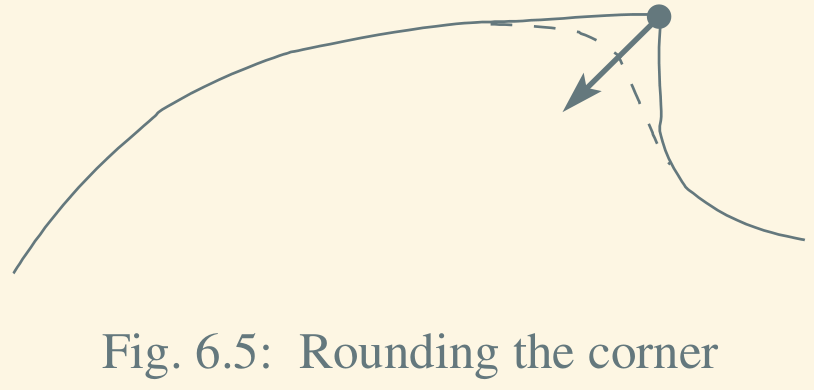
\includegraphics[width=0.3\textwidth]{fig3}
	\end{figure}
	so it would be nice to understand that precisely but \(\mathsf{OK}\). \textbf{Understood}: you take a uniformly normal neighbourhood of the point, then you can take radial geodesics spanning from other points in the neighbourhood, and you construct a shorter path around the corner.
\end{itemize}
\end{thing8}

So the \textit{\textbf{first variation formula}} in its full power version from \cite{ler} says
\begin{align*}
	\boxed{\begin{array}{rl}\frac{d}{ds}\Big|_{s=0}S(s)&=-\int_a^b\left<V,\ddot \gamma\right>-\sum_{i=1}^{k-1}\left<V(t_i),\dot\gamma(t_{i}^-)-\dot\gamma(t_{i}^+)\right>\\
				   & \qquad +\left<V(b),\dot\gamma(b)\right>-\left<V(a),\dot\gamma(a)\right>\end{array}}
	\end{align*}
\textbf{Explanation.} The first term we already know what it is. The second term is what happens at the singularities of the piecewise-smooth variation defined with singularities at \(t_1,\ldots,t_n\), and the third term is what happens at the first and final point.

\textbf{further explanation} \textit{the curve is piecewise smooth and the variation field is full smooth}. remember that, when you do the telescopic sum, if everything was smooth then the derivatives at the midpoints match and the midpoints would cancel, but if the velocities of the curve are not smooth then they don't match at the midpoints and you get those differences from the left and right. but the variation field is full smooth so that part matches and you can factor the thing.

So it remains kind of a mystery why Lee does the computations with the length functional and not with the energy functional. Ah! I think it's parametrization matters: for the formula above to work \textbf{you need unit speed}. I you don't have unit speed you don't get rid of the square root when differentiating, and that's terrible. So what everyone does is instead use the \textit{\textbf{energy functional}} which is just the integral of square of the norm,
\[\boxed{E(s)=\int_a^b |\dot \gamma|^2}\]
And what everyone does is that they show this doesn't mind parametrizations \textbf{and} that a geodesic is a geodesic iff it is a critical point of \(E\). That is, \(E\) still detects what you want it to detect, and it's easier to differentiate. And also has nothing to do with thermodynamics.
\section{second variation formula}

Here's  \cite{pet}. For good variations (smooth, fixing endpoints) of a geodesic \(\gamma\) it turns out that
\[\boxed{\frac{d^2}{ds^2}E(s)\Big|_{s=0}=\int_a^b |\dot V|^2- \int_a^b \left<R(V,\dot \gamma)\dot \gamma,V\right>}\]
where \(E\) is the energy functional.

And smooth version from \cite{pet} is
\[\boxed{\frac{d^2}{ds^2}E(s)\Big|_{s=0}=\int_a^b |\dot V|^2-\int_a^b \left<R(V,\dot \gamma)\dot\gamma,V\right>+\left<\nabla_{\partial_s}V,\dot\gamma\right>|_{a}^b}\]
But the full power version piecewise smooth from Florit lecture is something very similar to:
\begin{align*}
	\boxed{\begin{array}{rl}\frac{d}{ds}\Big|_{s=0}E(s)&=-\int_a^b\left<V,\ddot V+R(V,\dot \gamma)\dot \gamma\right>-\sum_{i=2}^{n-1}\left<V(t_i),\dot V(t^+_{i})-\dot V(t^-_{i})\right>\\
				   & \qquad +\left<V(b),\dot\gamma(b)\right>-\left<V(a),\dot\gamma(a)\right>+\left<\nabla_{\partial_s}V,\dot\gamma\right>|_{a}^b\end{array}}
	\end{align*}
which is more or less a useless formula since what do you want that for anyways. Meaning---use for application, not for the sake of knowing it or writing correctly or anything.

\section*{index}

We'll see eventually whether this turns out useful or forgotten. The \textit{\textbf{index form}} is
 \begin{align*}
	I_a: \mathfrak{X}_\gamma\operatorname{max}x \mathfrak{X}_\gamma &\longrightarrow \mathbb{R} \\
	I_a(V,W) &=\int_0^a \left<V',W'\right>-\left<R_{\gamma'}V,W\right>
\end{align*}

\section{minimal}
\subsection{first variation of a regular map to riemannian target}

Consider an isometric immersion \(f_0:(M,g) \to(\tilde{M},\tilde{g})\) and a vector field \(\xi \in f^*T\tilde{M}\).

Define a variation by:
\begin{align*}
	f: (-\varepsilon,\varepsilon)\times M &\longrightarrow \tilde{M} \\
	f(s,p) &=\operatorname{exp}_{p}(s \xi)
\end{align*}
Then \(f_s:=f(s,\cdot):M \longrightarrow \tilde{M}\) is an immersion (isometric at \(s=0\) by hypothesis). Now we define the \textit{\textbf{volume functional}} that simply computes the volume of \(M_s\):
\[S(s):= \int_{M}\operatorname{Vol}_{f_s ^*\tilde{g}}=\int_M f_s^*\operatorname{Vol}_{\tilde{g}}.\]
(\(S\) is physics notation and \(s\) is Florit notation.)

\begin{exercise}\leavevmode
Compute \(S'(0)\).
\end{exercise}
TL;DR. The derivative of the determinant is a trace, that trace is the trace of the shape operator, which is the mean curvature.

\begin{proof}[Solution]\leavevmode
How to express volume in any coordinate system?
\[\sqrt{\det (f^* _sg)_{ij}}dx^1\wedge\ldots\wedge dx^n\]
Let's differentiate:
\begin{align*}
	\frac{d}{ds}S(s)&=\frac{d}{ds}\int_M\operatorname{Vol}_{f^*_s\tilde{g}}=\frac{d}{ds}\int_M \sqrt{\det (f^* _sg)_{ij}}dx^1\wedge\ldots\wedge dx^n\\
&=\int_M \frac{d}{ds}\sqrt{\det (f^* _sg)_{ij}}dx^1\wedge\ldots\wedge dx^n
\end{align*}
We must differentiate the square root of the determinant of a matrix. 
%So let \(A(t)\) be any smooth 1-parametric family of matrices.
\[\boxed{\frac{d}{dt}\det A(t)=\det A(t) \cdot \operatorname{tr}\left(A(t)^{-1}\cdot \frac{d}{dt}A(t)\right)}\]
and using that we see that
\[\boxed{\frac{d}{dt}\sqrt{\det A(t)} =\frac{1}{2}\sqrt{\det A(t)} \cdot\operatorname{tr}\left(A(t)^{-1}\cdot \frac{d}{dt}A(t)\right) }\]
So we put \(A(s)=(f^*_s\tilde{g})_{ij}\). The good news is that square root of the determinant part is exactly the local coordinate function of \(\operatorname{Vol}_{f_0^*\operatorname{Vol}_{\tilde{g}}}=\operatorname{Vol}_g\). Then we only have to integrate that other function, which hopefully is related to the mean curvature.

Before computing recall the basic equations of submanifold theory: for \(X,Y \in \mathfrak{X}(M)\), \(\xi \in \Gamma(T^\perp M)\), \(\tilde{\nabla}\) L.C. connection of \(\tilde{M}\) and \(\nabla\) LC connection of \(M\) isometrically immersed in  \(\tilde{M}\), splitting everything into normal and tangent part we get
\[\boxed{\tilde{\nabla}^f_Xf_*Y:=f_*\nabla_XY+\alpha(X,Y)}\]
\[\boxed{\tilde{\nabla}_X^f g_*\xi:=-A_\xi f_*X+\nabla^\perp_X\xi}\]
and call \(\alpha\) the second fundamental form and \(A\) the shape operator. These two equations/definitions together imply
\[\boxed{\left<\xi,\alpha(X,Y)\right>=\left<-A_\xi X,Y\right>}\]


Let's compute
\begin{align*}
\frac{d}{ds}\Big|_{s=0}(f_s^*\tilde{g})_{ij}&=\frac{d}{ds}\Big|_{s=0}f_s^*\tilde{g}\left(\partial_i,\partial_j\right)=\frac{d}{ds}\Big|_{s=0}\tilde{g}(f^s_*\partial_i,f^s_*\partial_j)\\
&=\tilde{g}\left(\nabla^f_{\partial_s}f^s_*\partial_i,f^s_*\partial_j\right)+\tilde{g}\left(f^s_*\partial_i,\nabla^f_{\partial_s}f_*^s\partial_j\right)\Big|_{s=0}\\
&=\tilde{g}\left(\nabla^f_{\partial_s}f^0_*\partial_i,f_*^0\partial_j\right)+\tilde{g}\left(f^0_*\partial_i,\nabla^f_{\partial_s}f_*^0\partial_j\right)\\
&=\tilde{g}\left(\nabla^f_{\partial_i}f^0_*\partial_s,f_*^0\partial_j\right)+\tilde{g}\left(f^0_*\partial_i,\nabla^f_{\partial_j}f_*^0\partial_s\right)\qquad  \text{symmetry lemma} \\
&=\tilde{g}(\nabla^f_{\partial_i}\xi, f_*^0\partial_j)+\tilde{g}(f^0_*\partial_i,\nabla^f_{\partial_j}\xi)\end{align*}
Where \(\nabla^f\) is the pullback connection. The point is that we arrived at the variational field \(\xi\). If we assume (for now) that \(\xi\) is normal to \(M\) then upon differentiation we get:
\[\nabla^f_{\partial_i}\xi=-A_{\xi}\partial_i+N\]
where the normal component \(N\) vanishes since it is orthogonal to the basic tangent vectors of \(M\). We conclude that
\begin{align*}
\frac{d}{ds}\Big|_{s=0}(f_s^*\tilde{g})_{ij}&=\tilde{g}\left(-A_{\xi}\partial_i,\partial_j\right)+\tilde{g}\left(\partial_i,-A_{\xi}\partial_j\right)\\
&=\tilde{g}(\xi,\alpha(\partial_i,\partial_j))+\tilde{g}(\alpha(\partial_j,\partial_i),\xi)\\
&=2\tilde{g}(\xi,\alpha(\partial_i,\partial_j))\qquad\qquad \text{\(\alpha\) is symmetric}\\
&=-2\tilde{g}(A_{\xi}\partial_i,\partial_j)
\end{align*}
Now we have to multiply by the inverse matrix, which is just the inverse of the metric in \(M\) because we are at \(s=0\). Then we take trace and obtain the mean curvature, defined as the trace of the shape operator:
\begin{align*}
\operatorname{tr}\Big(g^{ij}g(A \partial_j,\partial_k)\Big)=g^{ij}g(A \partial_j,\partial_i)=g^{ij}g(A^\ell_j\partial_\ell,\partial_i)=g^{ij}A^\ell_jg_{\ell i}=\delta^{i}_jA^j_i=A^j_j
\end{align*}

We conclude
\[\frac{d}{ds}\Big|_{s=0}S(s)=-\int_M H \operatorname{Vol}_{g}\]
which says: \textbf{zeroes of the mean curvature function correspond to critical points of the volume functional}.
\end{proof}

\textbf{Addendum.} And the mean curvature vector? The mean curvature vector is \(H\xi\) for unit normal \(\xi\). And \(\tilde{g}(H\xi,\xi)=H\).
\section{jacobi field}

a \textit{\textbf{Jacobi field}} along a geodesic \(\gamma\) is \(J \in \mathfrak{X}_\gamma\) such that \(J''+R_{\gamma'}J=0\). 

Lembre que
	\begin{equation}\label{eq:segue}\dim\{J \in \mathfrak{X}^J_\gamma:J(0)=0, J \perp \gamma\}=n-1\end{equation}
Isso segue das seguintes observações:
\begin{enumerate}[label=(\alph*)]
\item \(\dim\mathfrak{X}^J_\gamma=2n\) porque são soluções de \(n\) equações diferenciais ordinárias de segunda ordem, i.e. cada campo de Jacobi está determinado pelas condições iniciais \(J(0)\) e \(J'(0)\). 
\item \(\dim \{J \in \mathfrak{X}^J_\gamma:J(0)=0\}=n\).
\item \(\dim \{J \in \mathfrak{X}^J_\gamma:J\perp \gamma'\}=2n-2\). Para confirmar isso note que pelas simetrias de \(R\) e a equação de Jacobi tem-se que \(\left<J,\gamma'\right>''=0\), pelo que \(\left<J,\gamma'\right>=a+bt\) para dois números reais \(a,b\). Segue que qualquer \(J \in \mathfrak{X}^J_\gamma\) se escreve como \(J(t)=a\gamma'(t)+bt\gamma'(t)+\hat{J}(t)\) para algum \(\hat{J}\) perpendicular a  \(\gamma'\). (Supondo que \(|\gamma'|=1\).) Então se \(J \perp \gamma\), temos que  \(a=b=0\), então tiramos dois números do \(2n\) que tínhamos.
\item Segue \cref{eq:segue}.
\end{enumerate}

Space of jacobi fields is thus of dimension \(2n\) since it any jacobi field is determined by initial conditions \(J(0)\) and \(J'(0)\). and the space of jacobi fields that vanish at the origin is just \(n\).

less obviously the space of jacobi fields orthogonal to  \(\gamma'\) is \(2n-2\) because: any jacobi field \(J\) can be written as
\[J=a+\gamma'+bt\gamma'(t)+\hat{J}\]
for some \(\hat{J}\perp \gamma\) and \(a,b \in \mathbb{R}\) such that \(\left<J,\gamma'\right>=a+bt\), and that's because \(\left<J,\gamma'\right>''=0\), so that's an affine real function \(a+bt\) for  \(a,b \in \mathbb{R}\). So the condition \(J(0)=a\gamma'(0)+bt\gamma'(0)\) says takes two numbers from the \(2n\) we already had.

finally if you look at the jacobi fields that are both perpendicular to \(\gamma'\) and \(J(0)=0\) you realise that \(a=0\) so the dimension of those is \(n-1\).

Just because I finally understood something about Jacobi field. A geodesic is given by \(\gamma_v(t)=\operatorname{exp}_p(tv)\) where \(p=\gamma(0)\) and \(v=\gamma'(0)\). Then choose a vector \(w \in T_pM\) and consider these lines:
\begin{figure}[H]
	\centering
	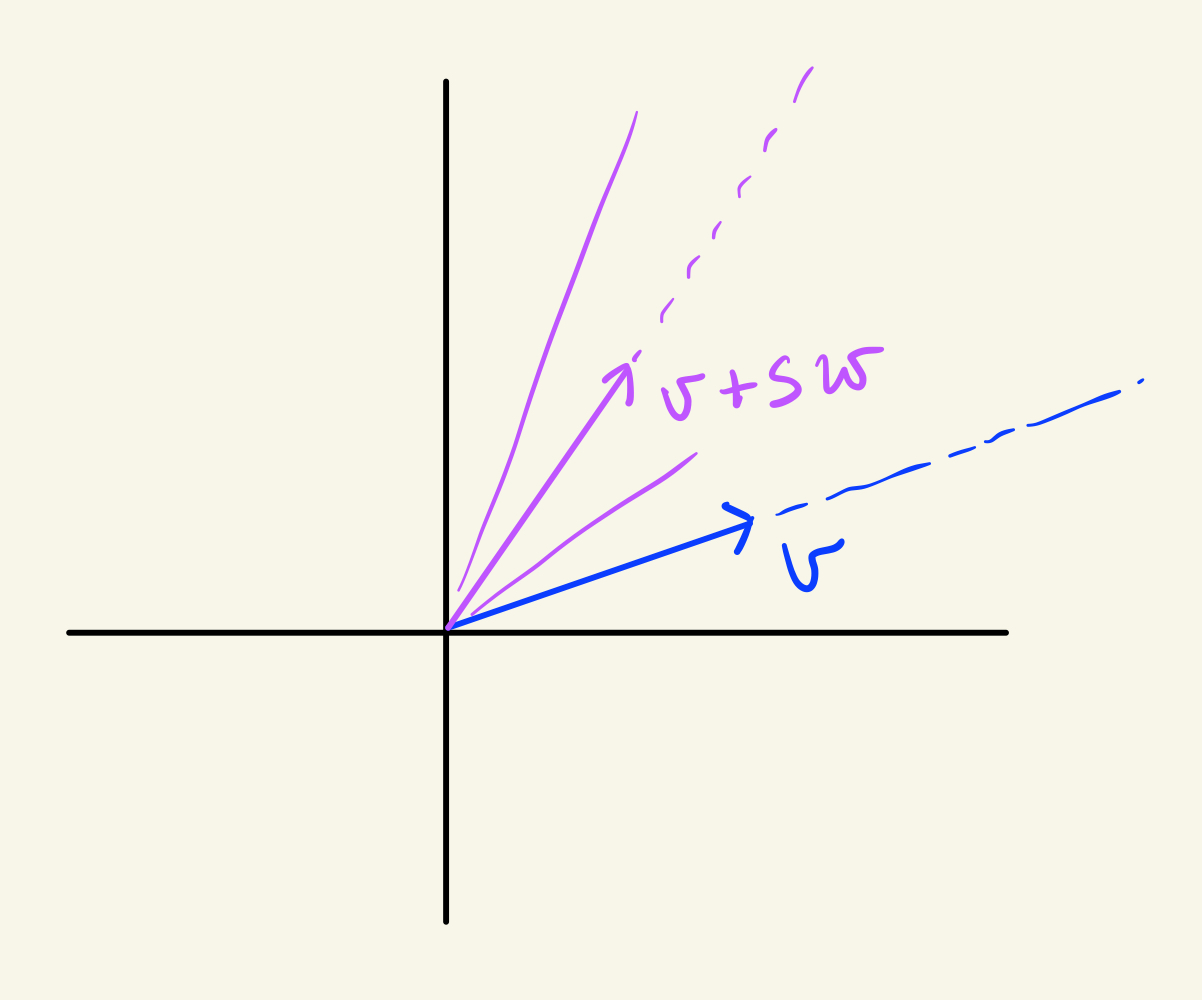
\includegraphics[width=0.4\textwidth]{fig2}
\end{figure}
Then taking \(\operatorname{exp}\) maps them to some geodesics. Then the \textit{\textbf{Jacobi field in this case}} is given by differentiating with respect to \(s\) along the curve \(tv\):
\begin{align*}\nabla_s \gamma_{v+sw}(t)&=\nabla_s \operatorname{exp}_p(t(v+sw))=d_{tv}\operatorname{exp}_p\cdot \frac{d}{ds}\Big(t(v+sw)\Big)\\&=d_{tv}\operatorname{exp}_p(tw).\end{align*}
And that's it.

That's not it. Given a variation of a geodesic \(\gamma\) by geodesics (this is even more general than above because we can vary the endpoints too), the variational vector field \(J \in \mathfrak{X}_\gamma\) satisfies the \textit{\textbf{jacobi equation}} 
\[J''+R_{\gamma'}J=0\]
where \(R_{\gamma'}V=R(V,\gamma')\gamma'\).

\subsection{a brutal exercise}

put yourself in the following situation: \(\gamma\) geodesic, \(v:=\gamma'(0)\), \(J \in \mathfrak{X}^J_\gamma\), \(J(0)=0\) (variation fixing endpoints), \(J'(0):=w\).

Up to this point \cite{au} says then \(J\) is como querias: \(J(t)=d_{tv}\operatorname{exp}_p(tw)\).

But I think we need more: \(J \perp \gamma'\) and probably also \(v \perp w\).

Then you can just do this: define \(g(s):=|J(s)|^2\) and differentiate \(g\) a lot:
\begin{align*}
g'(s)&=\frac{d}{ds}\left<J(s),J(s)\right>=2 \left<J'(s),J(s)\right>\\
g''(s)&=2\Big(\left<J''(s),J(s)\right>+\left<J'(s),J'(s)\right>\Big)\\
g'''(s)&=2 \Big(\left< J'''(s),J(s)\right>+\ldots
\end{align*}
Then you evaluate at \(0\) because you are computing Taylor at 0, realise so many things cancel, find \(R\) at \(g^{iv}\) and conclude that
\[|J(t)|^2=|w|^2t^2-\frac{1}{3}\left<R(w,v)v,w\right>t^2+O(t^4)\]

And then, some time after this in the course, all the way down to second variation formula and all that, you'll face
\begin{exercise}\leavevmode
\begin{itemize}
\item Show that \(d(\gamma_v(t),\gamma_w(t))=|v-w|t+O(t^2)\). Suggestion: consider the variation given by minimizing geodesics joining \(\gamma_c(t)\) and \(\gamma_w(t)\) for each small \(t\) and differentiate.
\item Use the previous exercise to show that \(\operatorname{Iso}(M,d)=\operatorname{Iso}(M,g)\).
\item Show that \(d(\gamma_v(t),\gamma_w(t))=|v-w|t-\frac{1}{6}\frac{\left<R(w,v)v,w\right>}{|v-w|}+O(t^4)\) but see equation 9 in \cite{mey}.
\end{itemize}
\end{exercise}


\section{riccati equation}

Take any point and any tangent vector at that point. Take the geodesic and take the geodesic sphere of raduis say \(\varepsilon\) with center in the point. It's a hypersurface. Normal vectors are all multiples of the unit normal vector. But who's that, the unit normal? Ah, it's the speed of the geodesic.



So? The normal derivative of any vector field tangent to the sphere w.r.t. the unit normal is…
\begin{align*}
0&=X\left<\nu,\nu\right>=2\left<\nabla^\perp_X \nu,\nu\right>
\end{align*}
that is, normal derivative of \(\nu\) w.r.t. \(X\) is perpendicular to \(\nu\), BUT normal derivative is normal so it's actually a multiple of \(\nu\), which makes \(\nu\) have norm zero or else \(\nabla^\perp_X \nu=0\).

Great! Now you take a variation \(f(s,t)\) which I think is our beloved Jacobi variation
\[d_{tv}\operatorname{exp}_p(sw)\]
and do
\begin{align*}
\nabla &= \ldots=J
\end{align*}
that is,
\[A(J)=J'\]
differentiate that or \(\overline{J}\) to obtain
\[A'+A^2+R_{\gamma'}=0\]

\section{curvature}

\subsection{curvature basics}

O \textit{\textbf{tensor de Ricci}} de \((M,g)\) é
\begin{align*}
	\operatorname{Ric}: TM \times TM &\longrightarrow  \mathbb{R}\\
	 \operatorname{Ric}(X,Y)&= \frac{1}{n-1}\operatorname{tr}(Z  \mapsto R(Z,X)Y)
\end{align*}
(É simétrico.)

A \textit{\textbf{curvatura de Ricci}} é
\begin{align*}
	\operatorname{Ric}: T_1M &\longrightarrow \mathbb{R} \\
	\operatorname{Ric}(X) &=\operatorname{Ric}(X,X)=\frac{1}{n-1}\sum_{i=1}^{n-1}K(X,E_i)
\end{align*}
onde \(E_i \perp X\), ou seja \(\{X,E_1,\ldots,E_{n-1}\}\) é uma base ortonormal.

A \textit{\textbf{curvatura escalar}} é
\begin{align*}
	\operatorname{scal}: M &\longrightarrow \mathbb{R} \\
	\operatorname{scal} &=\frac{1}{n}\operatorname{tr}\operatorname{Ric} 
\end{align*}

\begin{exercise}\leavevmode
\[\operatorname{scal}=\frac{1}{n}\sum_{i}\operatorname{Ric}(e_i,e_i)=\frac{1}{n(n-1)}\sum_{i+j}K(e_i,e_j)\overset{\text{exer} }{=}\frac{1}{\operatorname{Vol}\mathbb{S}^{n-1}}\int_{\sigma \subset T_pM}K(\sigma)\]
\end{exercise}

Curvature in constant sectional curvature \(c\) says
\[\left<R(X,Y)Z,W\right>=c\Big(\left<X,W\right>\left<Y,Z\right>-\left<X,W\right>\left<Y,Z\right>\Big)\]
which follows from… noticing that that function is so-called curvature-like i.e. satisfying the simmetries of \(R\) and that not immediate computation that any two curvature-like tensor with equal scalar curvatures must be equal themselves.

\subsection{pullback of curvature}

\begin{exercise}\leavevmode
\(f^* R=R_{\nabla^f}\)
\end{exercise}

\subsection{some facts about curvature}

\begin{claim}\leavevmode
\(M\) simplesmente conexa. Um fibrado a afim (i.e. munido de uma conexão) é isomorfo ao fibrado trivial iff \(R \equiv 0\).
\end{claim}



\begin{exercise}\leavevmode
Suponha que \((M_1,g_1)\) e \((M_2,g_2)\) são variedades Riemannianas e considere \(M_1\times M_2\) com a métrica produto \(g=g_1 \oplus  g_2\). Mostre que a curvatura Riemanniana, a curvatura de Ricci e a curvatura escalar de \(g\) são dadas pelas seguintes fórmulas:
\begin{enumerate}[label=(\alph*)]
\item \(R=\pi_1^*R_1+\pi_2^*R_2\)
\item \(\operatorname{Ric}=\pi_1^*\operatorname{Ric}_1+\pi_2^*\operatorname{Ric}_2\)
\item \(\operatorname{scal}=\pi_1^*\operatorname{scal}_1+\pi_2^*\operatorname{scal}_2\)
\end{enumerate}
\end{exercise}

\begin{proof}[Solução]\leavevmode
\begin{enumerate}[label=(\alph*)]
\item 
\end{enumerate}
\end{proof}

\subsection{curvature of CPn!}

\begin{thing6}{Exercício 1}[Curvatura do espaço projetivo complexo, \cite{doc} VIII.12]\label{exer:1}\leavevmode
Defina uma métrica Riemanniana  em \(\mathbb{C}^{n+1}\setminus\{0\}\) do seguinte modo. Se \(Z \in \mathbb{C}^{n+1}\setminus\{0\}\) e \(V,W \in T_Z (\mathbb{C}^{n+1}\setminus\{0\})\),
\[\left<V,W\right>_Z=\frac{\operatorname{Re}(V,W)}{(Z,Z)}\]
onde 
\[(Z,W)=z_0\overline{w}_0+\ldots+z_n\overline{w}_n\]
é o produto hermitiano em \(\mathbb{C}^{n+1}\). Observe que a métrica \(\left<\cdot,\cdot\right>\) restrita a \(S^{2n+1}\subset \mathbb{C}^{n+1}\setminus\{0\}\) coincide com a métrica induzida por \(\mathbb{R}^{2n+2}\).
\begin{enumerate}[label=(\alph*)]
\item Mostre que, para todo \(0\leq \theta \leq 2\pi\), \(e^{i\theta}:S^{2n+1}\to S^{2n+1}\) é uma isometria, e que, portanto, é possível definir uma métrica Riemanniana em \(\mathbb{P}^n(\mathbb{C})\) de modo que a submersão \(f\) seja Riemanniana.

\item Mostre que, nesta métrica, a curvatura seccional de \(\mathbb{P}^n(\mathbb{C})\) é dada por
\[\boxed{K(\sigma)=1+3\cos^2\varphi}\]
onde \(\sigma\) é gerado pelo par ortonormal \(X\), \(Y\), \(\cos \varphi=\left<\overline{X},i\overline{Y}\right>\), e \(\overline{X}\), \(\overline{Y}\) são os levantamentos horizontais de \(X\) e \(Y\), respetivamente. Em particular, \(1 \leq  K(\sigma) \leq  4\).
\end{enumerate}
\end{thing6}

\begin{proof}[Solução]\leavevmode
	Começo notando que a métrica \(\left<\cdot,\cdot\right>\) restrita a \(S^{2n+1}\) coincide com a métrica induzida por \(\mathbb{R}^{2n+2}\): pegue \(Z \in S^{2n+1}\) e \(V,W \in T_Z(\mathbb{C}^{n+1}\setminus\{0\}\). Então
	\begin{align*}
\left<V,W\right>_Z&=\operatorname{Re}( V,W)\\ &= \operatorname{Re}\sum v^i\overline{w}^i \\
&= \operatorname{Re}\sum \left(\operatorname{Re} v^i + \sqrt{-1}\operatorname{Im} v^i\right)\left(\operatorname{Re} w^i - \sqrt{-1} \operatorname{Im} w^i\right) \\
&= \operatorname{Re}\sum\left(\operatorname{Re} v^i\operatorname{Re} w^i + \sqrt{-1}(\operatorname{Im} v^i\operatorname{Re} w^i-\operatorname{Re} v^i\operatorname{Im} w^i ) + \operatorname{Im} v^i\operatorname{Im} w^i\right) \\
&= \operatorname{Re}\sum\left(\operatorname{Re} v^i\operatorname{Re} w^i + \operatorname{Im} v^i\operatorname{Im} w^i\right) + \operatorname{Re}\left(\sqrt{-1}(\dots)\right) \\
&= \sum \operatorname{Re} v^i\operatorname{Re} w^i + \operatorname{Im} v^i\operatorname{Im} w^i \\
&= \langle V,W\rangle_{\mathbb{R}^{2n+2}}
\end{align*}
\begin{enumerate}[label=(\alph*)]
\item Pela observação anterior, basta mostrar que \(e^{i\theta}\) é uma isometria de \(S^{2n+1}\) com a métrica esférica usual. Sabemos que o grupo de isometrias dessa esfera é \(\mathsf{O}(2n+2)\).

	De fato, o mapa \(e^{i\theta} \in \mathsf{O}(n+1,\mathbb{C})\subset\mathsf{O}(2n+2)\) onde o primeiro grupo são as isometrias da forma Hermitiana. Para ver por que, defina \(h\) como a forma hermitiana canônica de \(\mathbb{C}^{n+1}\). Das contas feitas acima fica claro que podemos escrever \(h=g+\sqrt{-1}\omega\), onde \(g\) é a métrica Riemanniana (produto ponto) canônica de \(\mathbb{R}^{2n+2}\) e \(\omega\) é uma outra forma bilinear.

Primeiro note que \(e^{i\theta}\) é uma isometria de \(h\). Para todo \(z \in \mathbb{C}^{n+1}\),
\begin{align*}
h(e^{i\theta}z,e^{i\theta}z)=e^{i\theta}\overline{e^{i\theta}}h(z,z)=|e^{i\theta}|^2h(z,z)=h(z,z)
\end{align*}
separando em parte real e imaginaria, segue que \(g(e^{i\theta}z,e^{i\theta}z)=g(z,z)\). Como \(e^{i\theta}\) é linear, concluímos que é uma isometria de \(g\).
\iffalse
	\textbf{(Ideia original.)}Pegue um vetor \(X(p) \in T_pS^{2n+1}\) e uma curva \(\gamma\) tal que \(\gamma'(0)=X(p)\). A derivada dessa curva depois de compor com \(e^{i\theta}\) vai ter o mesmo tamanho que \(X\) porque a derivada de \(\frac{d}{d\theta}e^{i\theta}=ie^{i\theta}\).

	\textbf{(Ideia de ChatGPT.)} Só note que \(e^{i\theta}\) é um mapa linear em \(\mathbb{C}^{n+1}\). Então a derivada dele é ele mesmo, que preserva o tamanho dos vetores por tratar-se de uma rotação. Aqui da para escrever \(e^{i\theta}\) como uma matriz em \(\mathcal{O}(2n+2)\).\fi
\item Seguindo a sugestão, defina \(N\) como o vetor de posição de \(S^{2n+1}\). Pensando \(\theta \mapsto e^{i\theta N}\) como uma curva usual em \(\mathbb{C}^{2n+1}\), sabemos pelas propriedades da exponencial complexa, i.e. derivando entrada a entrada, que \((\frac{d}{d\theta}e^{i\theta}N)_{\theta=0}=i N\).

	Esse vetor é vertical já que… (intento 1) \[\left<i N,N\right>=\operatorname{Re}h(i N,N)=\operatorname{Re}ih(N,N)=\operatorname{Re}i=0,\] mas esse argumento mostra que \(i N\) é ortogonal ao vetor posição, que é ortogonal ao espaço tangente da esfera, ou seja, que \(i N \in TS^{2n+1}\). Para mostrar que é vertical devemos ver que está no kernel da projeção \(\pi\). Isso está quase feito: como \(i N\) é a derivada de uma curva, basta compor essa curva com \(\pi\) e derivar em \(\theta=0\). O lance que no quociente essa curva é constante!

	Daí simplesmente escrevemos a fórmula de Manfredo para uma curva \(\alpha:(-\varepsilon,\varepsilon)\to S^{2n+1}\) realizando o levantamento \(\overline{X}\) de \(X \in \mathfrak{X}(\mathbb{C}P^{n})\) em \(N\), i.e. com \(\alpha(0)=N\) e \(\alpha'(0)=\overline{X}\):
	\begin{align*}
		(\overline{\nabla}_{\overline{X}}i N)_N&=\frac{d}{dt}i N \circ \alpha(t)\Big|_{t=0}\\
		&=\frac{d}{dt}i \alpha(t)\Big|_{t=0}\qquad  \text{ já que \(N\) é o vetor posição} \\
		&=i \alpha'(0)=i\overline{X}, \qquad \qquad \text{derivada complexa usual} 
	\end{align*}
	Agora note que
	\begin{align*}
	\overline{X}\cancelto{0}{\left<\overline{Y},iN\right>}&=\left<\overline{\nabla}_{\overline{X}}\overline{Y},i N\right>+\left<\overline{Y},\overline{\nabla}_{\overline{X}}i N\right>
	\end{align*}
	de modo que
	\begin{equation}\label{eq:cpn}
		\begin{aligned}
	\left<[\overline{X},\overline{Y}],i N\right>&=\left<\overline{\nabla}_{\overline{X}}\overline{Y}-\overline{\nabla}_{\overline{Y}}\overline{X},i N\right>\\
	&=-\left<i \overline{X},\overline{Y}\right>+\left<i \overline{Y},\overline{X}\right>\\
	&=2 \cos \varphi\end{aligned}
	\end{equation}
por definição de \(\varphi\) como satisfazendo \(\cos \varphi=\left<\overline{X},i \overline{Y}\right>\), e porque \[\left<i \overline{X},\overline{Y}\right>=\operatorname{Re}h(i\overline{X},\overline{Y})=\operatorname{Re}h(\overline{X},\bar{i} \overline{Y} )=\operatorname{Re}h(\overline{X},-i \overline{Y} )=-\left<\overline{X},i \overline{Y}\right>\]
Finalmente, o \textbf{exercício 10(b)} diz que para \(\sigma=\operatorname{span}\{X,Y\}\) e \(\overline{\sigma}=\operatorname{span}\{\overline{X}, \overline{Y}\}\),
\[\boxed{K(\sigma)=\overline{K}(\overline{\sigma})+\frac{3}{4}\left|\left[ \overline{X},\overline{Y} \right]^v\right|^2}\]
onde \(\overline{K}\) é a curvatura de \(\mathbb{S}^{2n+1}\setminus\{0\}\), que é constante 1. Portanto, o desafio final acaba sendo mostrar que
\[3 \cos^2 \varphi=\frac{3}{4}\left|\left[ \overline{X},\overline{Y} \right]^v\right|^2\]
Mas já tá quase: elevando \cref{eq:cpn} ao quadrado,
\begin{align*}
4\cos^2\varphi&=\left<\left[ \overline{X},\overline{Y} \right] ,i N\right>^2
\end{align*}
Ou seja, basta mostrar que
\[\left|\left[ \overline{X},\overline{Y} \right]^v\right|^2\overset{?}{=}\left<\left[ \overline{X},\overline{Y} \right],i N\right>^2\]
Como \(i N\) é vertical, o lado direito é igual a \(\left<\left[ \overline{X},\overline{Y} \right]^v, iN\right>^2\).

Como \(N\) é um vetor unitário, podemos expressar 
\[\left[ \overline{X},\overline{Y} \right]^v=\left|\left[ \overline{X},\overline{Y} \right]^v\right| i N\]
Então acaba que
\begin{align*}
\left<\left[ \overline{X},\overline{Y} \right]^v, iN\right>^2&=\left<\left|\left[ \overline{X},\overline{Y} \right]^v\right| i N, i N\right>^2=\left|\left[ \overline{X},\overline{Y} \right]^v\right|^2 \left<i N, i N\right>=\left|\left[ \overline{X},\overline{Y} \right]^v\right|^2
\end{align*}
\end{enumerate}
\end{proof}

\subsection{curvature under discrete quotients is preserved}
\begin{thing6}{Exercício 2}[Espaços lenticulares]\label{exer:2}\leavevmode
\begin{enumerate}[label=(\alph*)]
\item Definição e geodésicas (exer 4. cap. VIII \cite{doc}). Identifique \(\mathbb{R}^4\) com \(\mathbb{C}^2\) fazendo corresponder \((x_1,x_2,x_3,x_4)\) a \((x_1+ix_2,x_3+ix_4)\). Seja
	\[S^3=\{(z_1,z_2) \in \mathbb{C}^{2};|z_1|^2+|z_2|^2=1\}\]
	e seja \(h:S^3 \to S^3\) dada por
	\[h(z_1,z_2)=\left(e^{\frac{2\pi i}{q}}z_1,e^{\frac{2\pi i r}{q}}z_2\right) , \qquad  (z_2,z_2) \in S^3\]
	onde \(q \) e \(r\) são primos entre si, \(q>2\).
	\begin{enumerate}[label=(\roman*)]
	\item Mostre que \(G=\{\operatorname{id},h,\ldots, h ^{q-1}\}\) é um grupo de isometrias da esfera \(S^3\), com a métrica usual, que opera de modo totalmente descontínuo. A variedade \(S^3/G\) é chamada um \textit{\textbf{espaço lenticular}}.
	\item Considere \(S^3/G\) com a métrica induzida pela projeção \(p:S^3 \to S^3/G\). Mostre que todas as geodésicas de \(S^3/G\) são fechadas mas podem ter comprimentos diferentes.
	\end{enumerate}
\item Calcule o volume de um espaço lenticular.
\item Exiba uma sequência de variedades Riemannianas completas com curvatura seccional constante igual a 1 de modo que a sequência dos volumes seja uma sequência que converge a zero.

\end{enumerate}
\end{thing6}

\begin{proof}\leavevmode
\begin{enumerate}
	
	\item[(b)] Intuitivamente, o volume de um quociente é o volume do domínio fundamental, que é a região \(D\subset M\) mais pequena tal que \(G\cdot D=M\). Minha primeira ideia é pegar um ponto qualquer \(p \in S^3\) e todas as geodésicas partindo de \(p\). Para cada geodésica temos um tempo em que ela passa por um ponto que será identificado com \(p\) no quociente. A coleção desses pontos será o bordo do domínio fundamental.

Que complicações! Parece que a ideia é muito mais simples:
\[\operatorname{Vol}(S^3/G)|G|=\operatorname{Vol}(S^3)\]
no nosso caso, onde temos um grupo finito agindo por isometrias. Basta notar que \(|G|=q\), porque calcular o volume de \(S^3\) não é obvio e seguramente não faz parte do exercício.

\item[(c)] Lembre a pergunta: \textit{exibir uma sequência de variedades Riemannianas completas com curvatura constante igual a 1 de modo que a sequência dos volumes seja uma sequencia que converge a zero}. A resposta natural é \(S^3/G_q\) onde \(G_q\) é o grupo que determina o espaço lenticular, pudendo mudar o valor de \(r\) livremente desde que para cada \(q\) fique \(r\) primo relativo com \(q\).

	Então só falta mostrar que a curvatura secional de \(S^3/G\) é constante igual a 1, e que é completa. O último é imediato porque \(S^3\) é completa. Para ver o primeiro usamos de novo o exercício 10(b) que diz que para \(X,Y \in \mathfrak{X}(S^3/G)\), \(\sigma=\operatorname{span}\{X,Y\}\) e \(\overline{\sigma}=\operatorname{span}\{\overline{X}, \overline{Y}\}\),
\[\boxed{K(\sigma)=\overline{K}(\overline{\sigma})+\frac{3}{4}\left|\left[ \overline{X},\overline{Y} \right]^v\right|^2}\]
onde \(\overline{K}\) é a curvatura de \(S^3\), que \(1\). Ou seja, queremos ver que
\[\left[ \overline{X},\overline{Y} \right]^v=0.\]
Mas isso segue de que a ação é discreta! Temos uma descomposição \(TS^3 \cong \kappa \oplus  \pi^*T(S^3/G)\), onde \(\kappa\) é o kernel de \(\pi\). Como a dimensão do grupo é zero, a dimensão do espaço lenticular e 3, e o kernel dever ter dimensão zero. Então não tem componentes verticais em geral. Então aprendi que a curvatura seccional é preservada em quocientes sob ações discretas.
	
\end{enumerate}
\end{proof}

\subsection{boch equation}

\subsection{killing fields}

\section{isometric immersions}

\subsection{fundamental formulas of isometric immersions}
\(f:M \to \widetilde{M}\) isometric immersion. for \(X \in \mathfrak{X}(M)\) and \(\xi \in \mathfrak{X}_f=\Gamma(X,f^*  T \widetilde{M})\) you always have
\[\widetilde{\nabla}^f_X \xi=\left(\widetilde{\nabla}_X \xi\right)^\top+\left(\widetilde{\nabla}_X \tilde{Y}\right)^\perp\]
by decomposition of \(f^*T \widetilde{M} \cong TM \oplus \nu\).
\[\boxed{\widetilde{\nabla}_X^ff_*Y=f_* \nabla_XY+\alpha(X,Y)}\]
so you prove that the first factor is indeed the pushforward of Levi-Civita of \(M\) and that the second factor is a symmetric bilinear form (form?). Now if \(\xi \in T^\perp M\),
\[\boxed{\widetilde{\nabla}^f_X\xi:=-A_\xi X+\nabla^\perp_X\xi}\]
so you define the \textit{\textbf{shape operator}} as the tangent part of the derivative of a normal vector field, and the \textit{\textbf{normal connection}} as the normal part. And you prove \(\nabla^\perp\) is a connection.

\subsection{fundamental exercise of isometric immersions}

\begin{thing6}{Exercício L3.2}[Imersões isométricas]\label{exer:L3.2}\leavevmode
Seja \(f:M \to \overline{M}\) uma imersão isométrica. Sejam \(\nabla\) a conexão de Levi-Civita de \(M\) e \(\overline{\nabla}\) a conexão de Levi-Civita de \(\overline{M}\).
\begin{enumerate}[label=(\alph*)]
\item Let \(f:M^n \to \widetilde{M}^m\) be an isometric immersion and let \(\widetilde{\nabla}\) denote the connection on \(f^*T \widetilde{M}\) induced by the Levi-Civita connection of \(\widetilde{M}\). Verify that
	\[\nabla_XY=f^{-1}_*\left(\widetilde{\nabla}_X f_*Y\right)^\top\]
defines a compatible torsion-free connection on \(TM\), which therefore coincides with the Levi-Civita connection of \(M\).	

\item  (Reformulation of (a).) Mostre que
	\[f_*(\nabla_XY)=\left(\overline{\nabla}^f_Xf_*Y\right)_{TM}\]
e que essa igualdade determina \(\nabla\) em função de \(\overline{\nabla}\). Aqui, para \(W \in T_{f(p)}\overline{M}\), \(W_{TM}\) denota a sua projeção ortogonal ao subespaço \(f_*(T_pM) \subset T_{f(p)}\overline{M}\).
\item Seja \(c\) uma curva suave em \(M\). Mostre que para todo \(Y \in \mathfrak{X}_c\) vale
	\[f_*\nabla^c_{\frac{d}{dt}}Y=\left(\nabla^{f \circ c}_{\frac{d}{dt}}f_*Y\right)_{TM} \]
\item Seja \(\gamma:I \to M\) uma curva suave parametrizada pelo comprimento de arco. Mostre que \(\gamma\) é uma geodésica de \(M\) se, e somente se, sua aceleração em \(\overline{M}\) é perpendicular à variedade \(M\), i.e.,
	\[\overline{\nabla}^{f \circ \gamma}_{\frac{d}{dt}\Big|_{t}}(f \circ \gamma)' \perp f_*(T_{\gamma(t)}M)\]
	para todo \(t \in I\).
\end{enumerate}
\end{thing6}

\begin{proof}[Solução]\leavevmode
\begin{enumerate}[label=(\alph*)]
\item Nos han enseñado que esto se hace así (como dice la version de \cite{daj}): defina
	\[D: \mathfrak{X}(M)\times \mathfrak{X}(M) \longrightarrow \mathfrak{X}(M)\]
una conexión random pero satisfaciendo que
\[f_*(D_XY) = \left(\widetilde{\nabla}_X^f f_*Y\right)^\top\]
. Afirmamos que \(D\) es métrica y simétrica, o sea, \(D=\nabla\) y se acabó. (Que básicamente es el ``lema de simetría y compatibilidad".)
\begin{itemize}
\item \textbf{(Métrica.)} Se me antoja empezar con \(X\left<Y,Z\right>=\) pero ahí no sé que poner. (Puedo poner \(\nabla\) pero eso no sirve de nada.) Entonces mejor aplico \(f_*\), después de pensarlo me doy cuenta de que \(f_*Y\) y \(f_*Z\) son secciones de \(f^*\widetilde{M}\), o sea vectores en \(T\widetilde{M}\) pero como funciones están definidas em \(M\)! Acaba que lo que único que tiene sentido escribir es:
\begin{align*}
X\left<f_*Y,f_*Z\right>&=\left<\widetilde{\nabla}^f_Xf_*Y,f_*Z\right>+\left<f_*Y,\widetilde{\nabla}^f_Xf_*Z\right>
\end{align*}
\(\mathsf{OK}\) pero… eso es cierto? Bueno, lo que sabemos es que:
\begin{align*}
\left<\left( \widetilde{\nabla}^f_Xf_*Y\right)^\top,f_*Z\right>+\left<f_*Y,\left(\widetilde{\nabla}^f_Xf_*Z\right)^\top\right>&=\left<f_*(D_XY),f_*Z\right>+\left<f_*Y,f_*(D_XZ)\right>
\end{align*}



Ah, entonces eso es lo que hay que probar justamente. Me fijo en el lado izquierdo y digo bueno en cada punto, como \(f\) es isometría local,
\[\left<f_{*,p}Y(p),f_{*,p}Z(p)\right>_{f(p)}=\left<Y(p),Z(p)\right>_{p}\]
y como es un tensor escribo nomás
\[\left<f_*Y,f_*Z\right>=\left<Y,Z\right>\]
Y eso sí,
\[\left<Y,Z\right>=\left<\nabla_XY,Z\right>+\left<Y,\nabla_XZ\right>\]
No sé qué hacer con esos campos pero en campos coordenados sí, porque la base de  \(T_p\widetilde{M}\) es \(\partial_i\), pero eso no es una base del fibrado pullback, la que sí es base del fibrado pullback es \(\partial_i \circ f\). Ah entonces
\begin{align*}
\left<\widetilde{\nabla}_X^f \partial_i \circ f,\partial_i \circ f\right>+\left<\partial_j \circ f,\widetilde{\nabla}_X^f \partial_j \circ f\right>&= \left<\tilde{\nabla}_{f_*X}\partial_i,\partial_j\right>+\left<\partial_i,\widetilde{\nabla}_{f_* X}\partial_j\right>\\
&=f_*X\left<\partial_i, \partial_j\right>\\
&=X\left<\partial_i \circ f,\partial_j \circ f\right>
\end{align*}
\end{itemize}

\end{enumerate}
\end{proof}

\subsection{gcr}
\textit{\textbf{Gauss}}:
\[\left<\tilde{R}(X,Y)Z,W\right>=\left<R(X,Y)Z,W\right>-\left<\alpha(X,Z),\alpha(Y,W)\right>+\left<\alpha(X,W),\alpha(Y,Z)\right>\]
mira también puede ser así:
\[K_M(X,Y)=\tilde{K}(X,Y)+\left<AX,Y)\right>\left<AY,Y\right>-\left<AX,Y\right>^2\]
\begin{exercise}\leavevmode
use esa fórmula para mostrar que não pode ter \(M \hookrightarrow \mathbb{R}^{n+1}\) com curvatura negativa. Solução: porque Gauss diz que isso aí fica negativo mas do lado direito fica positivo porque os eigenvalores são \(0>\lambda_x\lambda_y\)
\end{exercise}

\textit{\textbf{Codazzi:}}

 \textit{\textbf{Ricci:}}

\section{amazing theorems}

\subsection{hopf-rinow}
\begin{thing6}{hopf-rinow}\leavevmode
São equivalentes
\begin{enumerate}[label=(\alph*)]
\item \(\operatorname{dom}\operatorname{exp}_p=T_pM\) 
\item Conjuntos fechados e limitados são compactos
\item \((M,d)\) é um espaço métrico completo
\item \(M\) é geodésicamente completa (toda geodésica está maximalmente definida em \(\mathbb{R}\))
\item Existem exhaustion
\end{enumerate}
Além disso, qualquer uma implica
\begin{enumerate}[label=(\alph*)]
	\item[(f)] \(\forall p,q \in M\) existe uma geodésica minimizante unindo eles.
\end{enumerate}
\end{thing6}

\subsection{hadamard}

\begin{thing6}{hadamard}\leavevmode
\(M\) completa, simplesmente conexa e \(K \leq  0\). Então, para todo \(p \in M\), \(\operatorname{exp}_p\) é um difeomorfismo global. Em particular \(M^n \overset{\operatorname{difeo}}{\simeq} \mathbb{R}^n\).
\end{thing6}

\begin{proof}\leavevmode
by you have a product/i have a product argument any two universal objects are isomorphic. so universal coverings are isomorphic. since \(M\) is simply connected it is its own universal cover. then we only need to show that also \(T_pM\) is a universal cover.

since \(K\leq 0\) we know \(\operatorname{exp}\) is a local difeo. but that doesn't say it is a cover. it has been claimed that a local diffeomorphism is a cover iff it lifts curves, but i don't know why the reverse is true (the direct implication is in hatcher).

to show \(\operatorname{exp}\) is a cover we pull the pullback metric to \(T_pM\). This makes \(\operatorname{exp}_p\) a local isometry. and there's a lemma:

\begin{thing6}{lemma 1}\leavevmode
If \(f:\tilde{M} \to M\) is a local difeo and \(\tilde{M}\) \textbf{is complete} and there is a number \(\varepsilon>0\) such that \(|f_*v|\geq \varepsilon|v|\) for all \(v\), then \(f\) is a cover map. The proof is showing that \(f\) lifts curves.
\end{thing6}
Nice, so the local isometry \(\operatorname{exp}_p\) satisfies that differential condition.

To finally show that \((T_pM, \operatorname{exp}_p ^*g)\) is complete we only notice that a the geodesics of \(T_pM\) with the new metric must be lines: the geodesics of the base are taken to lines and local isometry takes geodesics to geodesics. Lines on \(\mathbb{R}^n\) are curves maximally defined on all \(\mathbb{R}\).
\end{proof}

\begin{thing7}{lema 2}\leavevmode
Seja \(f:\tilde{M} \to M\) é um difeomorfismo local, onde \(\tilde{M}\) \textbf{é completo}, e suponha que \(|f_{*,p} v|\geq |v|\) para todo \(v \in T_pM\) e todo \(p \in M\). Então \(f\) levanta curvas e portanto é uma aplicação de recobrimento.
\end{thing7}
\begin{proof}[Prova do lema 2]\leavevmode
Suponha que uma curva \(\alpha:I \to M\) pode ser levantada a uma curva \(\tilde{\alpha}:[0,r) \to \tilde{M}\). Considere uma sequência \(t_n \to r\), e as sequências \(\alpha(t_n)\) e \(\tilde{\alpha}(t_n)\). Note que \(\alpha(t_n)\) é de Cauchy, pois \(\alpha(r)\) está bem definito. Então \(\tilde{\alpha}(t_n)\) também é de Cauchy:
\[d(\tilde{\alpha}(t_n),\tilde{\alpha}(t_m))\leq \int_{t_n}^{t_m} |\tilde{\alpha}'|\leq \int_{t_n}^{t_m}|f_*\tilde{\alpha}'|=\int_{t_n}^{t_m}|(f \circ\tilde{\alpha})'|=\int_{t_n}^{t_m}|\alpha'|\]
Quando \(n,m \to \infty\), o número da direita vai pra zero. Como \(\tilde{M}\) é completa, a sequência de Cauchy \(\tilde{\alpha}(t_n)\) é convergente a um ponto \(\tilde{\alpha}(r)\).

Isso mostra que o conjunto de parâmetros tais que \(\alpha\) pode ser levantada é fechado. Mas também é aberto: se \(\alpha(t)\) é levantado, como \(f\) é um difeomorfismo local, podemos levantar um vizinhança pequena de \(\alpha\) definindo-a como a imagem inversa local de \(f\).
\end{proof}

\begin{thing7}{observation}\leavevmode
Here's some discussion about why local diffeo is cover map iff it lifts curves: \href{https://math.stackexchange.com/questions/3122251/local-homeomorphism-curve-lifting-property-gives-a-covering-map}{StackExchange}.
\end{thing7}

\subsubsection*{hadamard for ricci and k3 surfaces}

\begin{exercise}\leavevmode
Remember Hadamard’s theorem? It says that a simply-connected, complete riemannian manifold with nonpositive sectional curvature is diffeomorphic to \(\mathbb{R}^n\).

Rumors say at some point in history of Florit’s class there was an exercise that says: change sectional curvature with Ricci curvature (in hadamard’s theorem) and show the statement is false.

A K3! It’s simply connected, complete, Ricci flat but compact.

Above idea sounds like an overkill—and even more in the context of a standard RG course hehe, but I cannot say I wouldn’t love to understand the details up to explaining them to RG monitor Ivan!

Anyway, if anyone finds it fun, Ivan would appreciate to have a good answer.
\end{exercise}
\begin{proof}\leavevmode
	The solution is basically showing that smooth K3 surfaces exist. So we may choose the easiest example, which is maybe a quartic surface in \(\mathbb{P}^3\). We have to explain in real riemannian geometry language what it is and why it is both simply connected and Ricci flat.
\begin{enumerate}[label=\textbf{Step \arabic*}]
\item Introduce the \textit{\textbf{Ricci form}} (prop. 8.30 \cite{lec}). This is nice: it's the classic version of Ricci form, i.e. trace of \(Z \mapsto R(Z,X)Y\), that in a kahler manifold may be expressed locally as
	\[\partial\bar\partial \operatorname{log} \det g\]
So (overkill starts?) save the proof of this fact, it shall be enough to show that this \((1,1)\)-form vanishes.	
	
\item Thm 8.31 \cite{lec} says: Ricci form is equal to \(2\pi\) times the first Chern form of the Chern connection on \(T'M\).
\item If we show that canonical bundle of our quartic is trivial (via adjunction formula) we are done. NO! I thought I could use this and never do Yau theorem but nope: this shows the \textit{cohomology} class of the Ricci form vanishes, but not that the Ricci curvature vanishes. So we'd have to solve Monge-Ampère (super-overkill) to find \textit{another} kahler metric whose ricci curvature truly vanishes.
\item We still have to show that the quartic is simply connected. Roughly, Misha's way is to define the smooth quartic as \(X \cap H\), a section of veronesse embedding of degree 4 \(\mathbb{P}^3 \to \mathbb{P}^N\) and take section with a hyperplane. And then hyperplane Lefschetz (final overkill) shows that \(\pi_{1}(X \cap H)=\pi_{1}(\mathbb{P}^3)\). \end{enumerate}
So maybe there's another way of showing simply connectedness at least? No super theorems? hahaha anyway… probably there's another solution…

\begin{enumerate}[label=\textbf{Step \arabic*}]
\item Say what it is. Choose a homogeneous quartic polynomial and define a submanifold of \(\mathbb{C}P^{3}\) as the zero-set function of the polynomial using inverse function theorem. You get a riemannian metric on the quartic induced from Fubini-Study, which I think at this point is most easily defined as the usual spherical metric on \(S^3\) passing down to the quotient under Hopf map. You have Levi-Civita connection, curvature, all the things in the classical RG story.
\item There's also the not-so-rg-classical-but-still notion of curvature matrix and curvature form, and first chern class which is basically curvature form up to a constant. Here we have to prove that this chern class is zero for the quartic we defined in step 1.
\item Introduce the \textit{\textbf{Ricci form}} (prop. 8.30 \cite{lec}). Note that Ricci form vanishes iff Ricci tensor vanishes i.e. manifold is Ricci flat in classical sense. That's what we want.
\item Thm 8.31 \cite{lec} says: Ricci form is equal to \(2\pi\) times the first Chern form of the Chern connection on \(T'M\).
\item Show that your favourite quartic surface in \(\mathbb{P}^3\) has vanishing first Chern class and is simply connected.
\end{enumerate}
\end{proof}

\subsection{lema de cartan}
\begin{thing6}{lema de cartan}\leavevmode
\[\begin{tikzcd}
	T_pM \arrow[r,"i"]\arrow[d,"\operatorname{exp}_p",swap]&T_p\tilde{M}\arrow[d,"\operatorname{exp}_{\tilde{p}}"]\\
	M\arrow[r,"f"]& \tilde{M}
\end{tikzcd}\]
tenemos una isometria entre los tangentes y queremos construir una isometria entre las variedades tal que \(d_pf=i\), o sea
\[f=\operatorname{exp}_{\tilde{p}}\circ i \circ \operatorname{exp}_p^{-1}\]
\textbf{lema} funciona si \(\phi^*\tilde{R}=R\)

	seja \(\phi:TU \to T\tilde{U}\) dado por
	\[\phi(P_{\gamma_v}(u))=\tilde{P}_{\gamma_{iv}}(iu)\]
	ou seja
	\[\phi=\tilde{P}_{\gamma_{iv}}\circ i \circ P_{\gamma_v} \qquad \forall v\]
	um isomorfismo de fibrados. Se \(\phi^*\tilde{R}=R\) então \(f=\operatorname{exp}_{\tilde{p}}\circ i \circ \operatorname{exp}_p^{-1}\) é uma isometria local.
\end{thing6}

\subsection{space forms}

\begin{thing6}{amazing theorem 8}\leavevmode
Seja \(M\) completa, simplemente conexa, com curvatura constante. Então \(M\) é globalmente isométrica a \(\mathbb{Q}^n_c\).
\end{thing6}

\subsection{bonnet-myers}

\begin{thing6}{bonnet-myers}\leavevmode
	\(M\) completa, \(\operatorname{Ric} \geq \frac{1}{r^2}\). Então \(\operatorname{diam}\leq \pi r\). Em particular \(M\) é compacta.
\end{thing6}
\begin{proof}\leavevmode
con pura segunda variación y un campo sinoidal
\end{proof}

\subsection{weinstein}
\begin{thing6}{Weinstein theorem}\label{thm:Weinstein theorem}\leavevmode
Seja \(M^n\) orientada, compacta, \(K>0\) e \(f \in \operatorname{Iso}(M)\).  Suponha que se \(n\) é par, \(f\) preserva orientação e que se \(n\) é ímpar \(f\) reverte orientação. Então \(f\) possui um ponto fixo.
\end{thing6}

\begin{proof}\leavevmode
       A fórmula da segunda variação é a fonte de inspiração, olhe:
\[E''(0)=\int |\dot V|^2-\int\left<R_ {\dot \gamma}V,V\right>+\left<\dot\gamma,\nabla_{\partial_s}f_s\right>|_{0}^a\]
e pense: o que preciso para tirar algo bacano dessa formulinha?

	De alguma maneira nos damos conta de que isso tem a ver com os pontos fixos de uma isometria \(f\). Suponha que \(f\) não tem pontos fixos e busquemos uma contradição. Defina
 \begin{align*}
	g: M &\longrightarrow \mathbb{R} \\
	g(q) &=d(q,f(q))
\end{align*}
então como \(M\) é compacta e essa função é contínua, ela tem um ponto mínimo que chamamos de \(p\). Temos que:
 \[0<g(p)=\operatorname{min}g\leq g(q)\qquad \forall q.\]
Vamos usar a segunda fórmula da variação para achar um ponto que avaliado em \(g\) fica menor do que \(g(p)\). Seja \(\gamma\) a geodésica minimizante entre \(p\) e \(f(p)\) parametrizada por comprimento de arco (que existe porque \(M\) compacta implica completa).

Agora pegue um vetor \(v \in T_pM\) unitário e ortogonal a \(\dot \gamma\) (para que o termo com \(R\) na fórmula da seg. var. fique \(K\)), transporte ele paralelamente ao longo de \(\gamma\) para obter \(V\), e pegue a variação por geodésicas
\[h(s,t)=\operatorname{exp}_{\gamma(t)}(sV(t))=\gamma_{V(t)}(s).\]
Então a 2nda fórmula fica beleza: como o campo é paralelo, o termo \(|\dot V|^2\) morre, o termo da curvatura fica \(K\) e o termo com \(\nabla_{\partial_s}f_s\) morre também (porque as curvas verticais são geodésicas).

Então como estamos em \(K>0\), acaba que \(E''(0)<0\), então existe uma vizinhança de \(0\)  onde as curvas \(f(s,t)\) tem menor energia que \(f(0,t)\) (para toda \(s\) nessa  vizinhança). Agora lembre que a \(\ell^2 \leq dE\), e que no caso de geodésicas minimizantes se da a igualdade. Então fica que
\[\frac{1}{d}\ell^2(c^s)\leq E(s)<E(0)=\frac{1}{d}\ell(\gamma)^2=\frac{1}{d}d(p,f(p))^2=\frac{1}{d}(\operatorname{min}g)^2\]
onde \(d=g(p)=d(p,f(p))\). Para chegar numa contradição precisamos obter \(g\) no lado esquerdo. Defina \(\beta(s)\) como a curva ``vertical" no tempo 0, ie. \(\beta(s)=f(s,0)\). Queremos mostrar que
\[\boxed{\frac{1}{d}d(\beta(s),f(\beta(s))^2\leq \frac{1}{d}\ell^2(c^s)}\]
Já que por definição, do lado esquerdo temos \(\frac{1}{d}g(\beta(s))^2\), dando uma contradição com a equação anterior. Para confirmar essa desigualdade e concluir a prova só devemos mostrar que a curva \(c^s\) liga \(\beta(s)\) e \(f(\beta(s))\), pois a distância entre esses dois pontos é menor do que o comprimento de qualquer curva que liga esses pontos.

Ou seja, queremos que
\[c^s(0)=\beta(s),\qquad c^s(d)=f(\beta(s))\qquad \forall s\]
Ou seja, queremos que
\[f \circ \beta=\gamma_{V(d)}\]
Note que \(\beta(s)=\gamma_{V(0)}(s)\). Então derive em \(s=0\): 
\[f \circ \beta=f\circ\gamma_{V(0)}=\gamma_{V(d)}\iff f_{*,p}V(0)=V(d)=PV(0)\]
onde \(P\) é o transporte paralelo ao longo de \(\gamma\) de \(p=\gamma(0)\) a \(\gamma(d)\).
Isso implica que queremos que
\[P^{-1}f_{*,p}V(0)=V(0)\]
Com um desenho muito convincente (ver Manfredo p. 225, esse agumentinho tá tranquilo) fica que como \(f\) é uma isometria
\[f_{*,p}\gamma'(0)=\gamma'(d)\]
Decorre daí que \(P^{-1}f_{*,p}\gamma'(0)=P^{-1}\gamma'(d)=\gamma'(0)\). Então podemos fixar nossa atenção em
\[A:=P^{-1}f_{*,p}|_{\gamma'(p)^\perp}\in \mathsf{O}(n-1)\]
Nosso objetivo é analisar o que acontece quando \(A\) tem um ponto fixo, \(V(0)\), pois essa é uma condição que queremos que seja verdade para que \(f\circ \beta = \gamma_{V(d)}\).

Agora segue o argumento dos eigenvalores que diz assim. Defina \(A:=P^{-1}f_{*,p}\). Suponha que \(A\) tem um ponto fixo. Os autovalores vem dados assim:
\[\operatorname{Spec}A=\{\underbrace{\lambda_1,\overline{\lambda_1},\lambda_2,\overline{\lambda_2}}_{\text{par} },-1,\ldots,-1,1,\ldots,1\}\]
Ou seja, os eigenvalores que não são 1 ou \(-1\) não afetam o determinante. Daí concluímos que
\begin{itemize}
\item Se \(n-1\) é ímpar, \(f\) preserva orientação. Por que? Deixa os complexos do lado que não importam. Então pensa: se só tenho \(-1\)s, então tenho uma quantidade ímpar de \(-1\)s porque a dimensão é ímpar. Respira. Nesse caso \(f\) inverte orientação. Mas: \(f\) deve ter pelo menos um \(1\)! Então a quantidade de \(-1\)s  é par. Então não: \(f\) preserva orientação.
\item se \(n-1\) é par, \(f\) reverte orientação.
\end{itemize}
E essas são as condições que precisamos para que \(A\) tenha um ponto fixo e tudo funcione. Então bota isso aí na hipótese do teorema.
\end{proof}

\subsection{synge}

\begin{thing6}{Synge theorem}\leavevmode
\(M^n\) compact, \(K>0\).
 \begin{enumerate}[label=(\roman*)]
\item Se \(n\) é par, \(\pi_{1}(M)=\begin{cases}
	1\qquad &\text{ se \(M\) é orientável}  \\
	\mathbb{Z}_2\qquad &\text{ se não} 
\end{cases}\) 
\item Se \(n\) é ímpar, \(M^n\) é orientável.
\end{enumerate}
\end{thing6}

\subsection{jacobi theorem}

\begin{thing6}{jacobi theorem}\leavevmode
\(\gamma:I \to M\) geodésica, \(\gamma(a)\) conjugado a \(\gamma(b)\) ao longo de \(\gamma\) \(\implies\) \(\forall \delta>0\), \(I_{a+\delta}\not \geq 0\). ou seja, \(\gamma\) não minimiza depois do primeiro ponto conjugado (cf. teorema do indice de morse).
\end{thing6}
\begin{proof}\leavevmode
con pura segunda variación
\end{proof}

\subsection{index lemma}

\begin{thing6}{index lemma}\leavevmode
Se \(\gamma\) não tem pontos conjugados \(\forall V \in \mathfrak{X}_\gamma\) dif por partes, \(V(0)=0\) então
	\[\boxed{I_a(J,J) \geq I_a(J,J)}\]
para \(J \in \mathfrak{X}^J_\gamma\), \(J(0)=0\), \(J(a)=V(a)\). Vale \(=\) \(\iff\) \(V=J\).
\end{thing6}
\begin{proof}\leavevmode
the idea is that because there are no conjugate points along \(\gamma\) we can take a basis of jacobi fields. then we get super cumberstone computations
\end{proof}

\subsection{sturm theorem}

\begin{thing6}{sturm}\leavevmode
	Dos funciones \(f\) y \(\tilde{f}\) definidas en \([0,a] \to \mathbb{R}\).
	Otras dos funciones \(K\), \(\tilde{K}\) definidas en \([0,a]\). \textbf{Importantemente,} \(\tilde{f}>0\). Ahora las condiciones iniciales son
	\[f(0)=0, \tilde{f}(0)=0, \qquad f'(0)=\tilde{f}(0)\]
y bueno
\[f''+Kf=0, \qquad  \tilde{f}''+\tilde{K}\tilde{f}=0\]
Se \[\tilde{K} \geq K\], entonces \(f/\tilde{f}\) é não decreciente, que implica que \(\tilde{f} \leq  f\).

Além disso se para algum \(t \in (0,a]\) se satisface que \(f(t)=\tilde{f}(t) \implies  f\equiv\tilde{f}\) e \(K\equiv\tilde{K}\) em \([0,t]\).
\end{thing6}

\subsection{rauch}

\begin{thing6}{rauch}\leavevmode
	Dos geodésicas creo que unitarias, pero en variedades distintas, y un campo de Jacobi en cada una. \textbf{\(\tilde{\gamma}\) no tiene puntos conjugados}. Los campos de Jacobi son parecidos en cuanto a que
	\[J(0)=0, \tilde{J}(0)=0, \qquad \left<J,\gamma'\right>=0=\left<\tilde{J},\tilde{\gamma}'\right>,\qquad |J'(0)|=|\tilde{J}'(0)|\]
Si
\[K\leq \tilde{K}\]
entonces
\[|\tilde{J}|\leq |J|\]
 \begin{align*}
\begin{aligned}
	\gamma:[0,a] \longrightarrow M^n \qquad &J\\
	\tilde{\gamma}:[0,a] \text{ SPC} \longrightarrow \tilde{M}^m \qquad &\tilde{J}
\end{aligned}\qquad K \leq \tilde{K} \implies \|J\| \geq \|\tilde{J}\|
\end{align*}
\[K(\gamma',J) \leq \tilde{K}(\tilde{\gamma};,\cdot)\qquad \frac{\|J\|}{\|\tilde{J}\|}\text{ é crescente} \]
Além disso, se para algum \(t \in (0,a]\) se satisface que \(\|J(t)\|=\|\tilde{J}(t)\|\) entonces \(\|J\|\equiv\|\tilde{J}\|\), \(K(\gamma',J)\equiv K(\tilde{\gamma}',\tilde{J})\) em \([0,t]\).
\end{thing6}
\begin{proof}\leavevmode
con lema do índice
\end{proof}

\subsection{codimensão em curvatura negativa: otsuki lemma e moore}

\begin{thing6}{otsuki lemma}\leavevmode
\end{thing6}

\begin{thing6}{corolário}\leavevmode
\(M^n \subset \tilde{M}^{n+p}\), \(K < \tilde{K} \implies p \geq n-1\).
\end{thing6}

\begin{thing6}{moore}\leavevmode
No contexto do lema de cartan, \(M^n \subset \tilde{M}^{n+p}\) subvariedade compacta, \(\tilde{M}\) hadamard, \(K \leq  \tilde{K} \leq 0 \implies p \geq n\).
\end{thing6}

\subsection{superprop de comparação aka toponogov local}

\begin{thing6}{superprop}\leavevmode
seja \(f\) a isometria do lema de cartan. \(K \leq  \tilde{K} \implies \) \(f\) é uma contração, i.e. \(\|f_*\|\leq  1\). Bastará com \(K(\gamma'_v,\cdot)\leq \tilde{K}(\tilde{\gamma}'_{iv},\cdot)\)? Além disso, se \(B\) é convexa então \(f\) é uma contração métrica.
\end{thing6}

\begin{thing7}{toponogov local is when \(B\) is convex}\leavevmode
you have two hinges. a hinge is just two geodesics \(\gamma_0\), \(\gamma_1\) that emanate from a point, and a number that is the angle \(\alpha\) between them. So really its two vectors and a number. maybe even just  three numbers.

the other hinge is \(\tilde{\gamma}_0\) and \(\tilde{\gamma}_1\) and \(\tilde{\alpha}\), and it is in another manifold \(\tilde{M}\) with \(K \leq  \tilde{K}\).

then for any \(s,t\) 
\[\tilde{d}(\tilde{\gamma}_0(t),\tilde{\gamma}(s)) \leq d(\gamma_0(t),\gamma_1(s))\]
\end{thing7}

\textbf{explicação:} se \(K \leq  \tilde{K}\) então \(d \geq \tilde{d}\) onde \(d,\tilde{d}\) são os lados opostos de triângulos com mesmo angulo e lados adjacentes do mesmo tamanho.

\begin{proof}\leavevmode
the two hinges determine an isometry \(i\) (not uniquely, but there's an isometry) between the tangent spaces. then there's a map, like in cartan theorem but the result and the point of cartan theorem has nothing to do with this,
 \[f=\operatorname{exp}_{\tilde{p}}\circ i \circ \operatorname{exp}_p^{-1}\]
coming from
\[\begin{tikzcd}
	T_pM \arrow[r,"i"]\arrow[d,"\operatorname{exp}_p",swap]&T_p\tilde{M}\arrow[d,"\operatorname{exp}_{\tilde{p}}"]\\
	M\arrow[r,"f"]& \tilde{M}
\end{tikzcd}\]
now's a good time to notice that the ``differential" version of the toponogov local theorem, i.e. before taking distances, is just the superprop, that is, that \(|f_*w|\leq |w|\).

but whose \(w\)? \(w\) is any vector inside \(B\). lit. and then you just take a random geodesic emanating from \(p\) reaching the point \(w\) is tangent to (ok there's only one such geodesic). and make up a jacobi field with mastery and simplicity
\[J(t)=d_{tw}\operatorname{exp}_p(tw')\]
and then you push \(w\) forward using \(f\) and with mastery and simplicity notice you have in your hands a jacobi field on the other side:
\[f_*w=d_{?}\operatorname{exp}_{\tilde{p}}(\underbrace{di}_{=i}(d_?\operatorname{exp}_p^{-1}w))=d_{iw}\operatorname{exp}_{\tilde{p}}i w'=\tilde{J}\]
since \(i\) is an isometry you are in position of applying rauch, and conclude that
\[|f_*w|=|\tilde{J}|\leq |J|=|w|\]
\hfill and toponogov and the triangles?

ah, you go metric, ie. suppose \(B\) is convex, integrate to get the distances, that's simple, and that's it. what

yes: your hinges gave you an isometry. your isometry gave you a function. \textbf{your function maps the hinge to the other hinge}, so it helps you compare the points on the domain with the points on the codomain. your function is a contraction.\end{proof}

\subsection{pontos focais}

It's a Jacobi field that the curves \(c^s\) arrive perpendicularly at the submanifold \(N\). Also the curve \(\beta(s)=f(s,0)\) is contained in the submanifold \(N\). And \(J(r)=0\) for some \(r\). This is supposed to be equivalent to 
\[J(0) \in T_p N\qquad  \text{and} \qquad J'(0)+A_{\gamma'(0)}J(0) \in T_p^{\perp}N\]
Ou seja: \(q \in M\) is a \textit{\textbf{focal point}} de \(N\) (ao longo de \(\gamma\)) se \(\gamma\) é uma geodésica unindo \(N\) e \(q=\gamma(r)\), \(\gamma'(0) \perp N\), existe \(0 \neq  J \in \mathfrak{X}^J_\gamma\) satisfazendo isso que tá na caixa e tal que \(J(r)=0\).

\begin{prop}\leavevmode
singularidades de \(\operatorname{exp}^\perp:=\operatorname{exp}|_{T^\perp N}\) são os pontos focais de \(N \subset M\).
\end{prop}

\begin{thing6}{teorema de hermann}[not in proved]\leavevmode
\(N \subset M\), \(N\) fechada e \(M\) completa, \(\operatorname{Foc}(N \subset M)=\varnothing\) então \(\operatorname{exp}^\perp\) é aplicação de recobrimento
\end{thing6}

\subsection{morse index}

\begin{thing6}{índice de morse}\leavevmode
o índice \(i(I_t)\) é finito e igual ao número de pontos conjugados em \([0,t)\) ao longo de \(\gamma\).
\end{thing6}
the problem is that the vector spaces of sections of smooth manifolds are infinite-dimensional. we are interested in computing
\[i(I_a):=\operatorname{sup}\{\dim L \subset \mathfrak{X}_\gamma:I_a |_{L \times L}<0\}\]
which is just the usual index or signature of a bilinear form. But how to compute that if the vector space is monstrous.

the index form
\[I_a:\mathcal{V}_a \times \mathcal{V}_a \longrightarrow \mathbb{R}\]
where
\[\mathcal{V}_a:=\{V \in \mathfrak{X}_\gamma \text{piecewise diff, }V(0)=0,V(a)=0\}\]
is hard to deal with.

so we chose a partition of the piecewise differentiable \(\gamma\) and define
\[\mathcal{V}_t^+:=\{V \in \mathcal{V}_t: V(t_i)=0\}\]
\[\mathcal{V}_t^-:=\{V \in \mathcal{V}_t:V|_{[t_j,t_{j+1}}\in \mathfrak{X}^J_{\gamma|_{[t_j,t_{j+1}}}\}\]
so yes, the \(-\) part is the jacobi fields, who save the day. and they \textit{do} save the day---because they are a priori not involved in this problem: the index form is really just the second variation formula. so when did jacobi fields appear? \textit{it's just curvature after all}

now there are three key observations:
\begin{enumerate}
\item \(\mathcal{V}_t=\mathcal{V}_t^+ \oplus  \mathcal{V}_t^-\)
\item \(\mathcal{V}_t^- \cong \bigoplus_{j=1}^{i-1}T_{\gamma(t_j)}M:=S\). {\color{2}i think} this is because we are in jacobi fields with first initial condition equal to zero. which means that every copy of \(T_{\gamma(t)}M\) is for the other initial condition \(J'(t)\).
\item \(\ker I_t:=\{V \in \mathcal{V}_t:I_t(V,W)=0 \forall W \in \mathcal{V}_t\}=\mathcal{V}_t \cap \mathfrak{X}_\gamma^J\)
this one says that \textbf{the kernel of \(I_t\) is the jacobi field part} (it is inside the set of all jacobi fields). that's because second variation formula. so \textbf{the dimension of the kernel is what we call multiplicity} of \(\gamma(t)\) and \(\gamma(0)\) as conjugate points.
\item \(I_t|_{\mathcal{V}^+_t \times \mathcal{V}^+_t}>0\) because for \(V \in \mathcal{V}^+_t\), \(I_t(V,V)=\sum_{j=1}^{i+1}I_{\gamma|_{t_{j-1},t_j}}(V|_{[t_{j-1},t_j]},V|_{[t_{j-1},t_j]}{\color{2}\geq I(0,0)=0}\). This one is by index lemma! twice!
\item \(I_{t}(\mathcal{V}_t^-,\mathcal{V}_t+)=0\).
\item so we conclude that
	\[\begin{array}{c}
	\mathcal{V}_t^-\\
	 \mathcal{V}_t^+\end{array}\left(\begin{array}{@{}c|c@{}}
	&0\\
	\hline
	0&>0\end{array}\right)\]
meaning that the \textbf{index is the index on the jacobi field part \(\mathcal{V}^-_t\)} and in particular it is finite:
\[i(I_t)=i(I_t|_{\mathcal{V}_t^- \times \mathcal{V}_t^-}<\infty\]
which is great. but it is not still clear what is the relationship with that and the kernel of \(I_t\) (and conjugate points).
\item then comes a function \(\varphi\) that i don't know what it does
\item now let \(L\) be the subset of \(S\) (which, if you recall, is just \(j-1\) copies of  \(T_{\gamma(t)}M\), one for each initial condition \(J'(0)\)) such that
	 \[I_{t}|_{L \times L}>0\]
so that
\[\dim L=\dim S-i(t)-\mathcal{V}(t)\]
which is just because \(S\) is split as: the part where \(I_t\) is positive definite, where it is negative definite, and where it is zero. \textbf{não tem mistério}
\item then comes the \(\varphi\). looks like
\begin{enumerate}[label=(\alph*)]
\item \(\varphi\) preserves the index: \(i(I_t)=i(\varphi_t^*I_t):=i(\hat{I}_t)=i(t)\). So there's another index form
	\begin{align*}
		\hat{I}_t: S \times S &\longrightarrow \mathbb{R} \\
		\hat{I}_t(U,V) &= I_t(\varphi u,\varphi v)
	\end{align*}
\item So maybe now it makes sense that
	\[\varphi_{t'}:S \overset{\operatorname{iso}}{\longrightarrow}\mathcal{V}_{t'}^-\]
	contínuas para toda \(|t'-t|<\varepsilon\).
\item So there's a bunch of these \(\varphi\) things.
\end{enumerate}
\item \(\mathsf{OK}\) back to earth take \(V \in L\) so that \(\hat{I}_t(V,V)>0\). but hey that says that
	\[\hat{I}_{t+\delta}(V,V)=I_{t+\delta}(\varphi_{t+\delta}V,\varphi_{t+\delta}V\]
\item then he erases that and instead puts
	\[\exists  \delta>0: |t-t'|<\delta \implies I_{t'}|_{L \times L}>0\]
	 {\color{2}which makes no sense} because \(I_{t'}\) should be positive on \(L \times L\) anyways…

	 and that means that
	 \[i(t') \leq \dim S- \dim L=i(t)+\mathcal{V}(t)\]
	 mmm… something like \textit{near \(t\), the index is smaller than the index plus the nullity} 
\item Final step: apply index lemma to show that
	\[\hat{I}_t > \hat{I}_{t+\varepsilon}\text{ em } \ker I_t\]
which says that for small \(\varepsilon>0\) 
\[i(t+\varepsilon)\geq  i(t)+\mathcal{V}(t)\]
so that
\[\boxed{i(t+\varepsilon)=i(t)+\mathcal{V}(t)}\]
\( \forall t \in [0,a]\) and  \(\varepsilon\) pequeno. and that proves the theorem
	
\end{enumerate}
\textbf{why?}


\begin{coro}\leavevmode
as geodésicas não minimizam depois do primeiro ponto conjugado. de fato, \(I_a \not\geq 0\iff\exists t\in[0,a)\) conjugado a \(\gamma(0)\) ao longo de \(\gamma\).
\end{coro}

\begin{coro}\leavevmode
pontos conjugados são discretos
\end{coro}

\subsection{bishop-gromov}

\begin{thing6}{bishop-gromov}\leavevmode
\(\operatorname{Ric}\geq k \implies \operatorname{Vol}(B_t(p))/\operatorname{Vol}(B_{t,k})\) decrescente para todo \(0 \leq  t \leq  i(p)\) onde \(i(p) =d(p,C_m(p))\) é o raio de injetividade de \(\operatorname{exp}\).
\end{thing6}

\begin{proof}\leavevmode

\end{proof}

\subsection{cheng}
bonnet-myers says: ricci bounded by \(k\) \(\implies \) \(\operatorname{diam}\leq \pi k\). This says
\begin{thing6}{cheng theorem}\leavevmode
If \(\operatorname{diam}M^n=\pi k\) then \(M\) is isometric to \(S^n_k\), ou seja espaço de curvatura constante \(1/k^2\).
\end{thing6}

\begin{proof}\leavevmode

\end{proof}

\subsection{calabi-yau}

\begin{thing6}{calabi-yau, 1975}\leavevmode
\(M^n\) complete and noncompact, \(\operatorname{Ric}_M \geq 0 \implies\)\[operatorname{Vol}(B_r(p)) \geq r \frac{\operatorname{Vol} B_{r_0}(p)}{2^{n+3}r_0}\qquad \text{if } r\geq 6r_0\]
that thing is a constant so this just says that \(\operatorname{Vol}B_r(p)\) grows linearly in \(r\).
\end{thing6}


\clearpage
\chapter{ag algebraic geometry}

\begin{quotation}
	the sea advances insensibly in silence, nothing seems to happen, nothing moves
\end{quotation}

\section{algebraic variety}

An \textit{\textbf{algebraic variety}} is a compact topological space equipped with a ring of sheaves which is locally isomorphic to an affine variety with its sheaf of regular functions and Zariski topology.

Amazing! An affine variety? Sure, it's \(Z\), the solution set of some polynomial equations on \(\mathbb{C}^n\) equipped with the ring of algebraic functions, which are the restrictions of polynomial functions to \(Z\). Zariski topology? Sure, closed sets are solution sets of polynomial equations.

Compare with \cite{gri}, p. 12: a subset \(V\) of an open set \(U \subset \mathbb{C}^n\) is an \textit{\textbf{analytic variety}} in \(U\) if for any \(p \in U\) there exists a neighbourhood \(U'\) of \(U\) such that \(V \cap U'\) is the common zero locus of a finite collection of \textit{holomorphic} functions on \(U'\).

And compare with \cite{gri}, p. 128: an \textit{\textbf{algebraic variety}} is defined to be the set of complex zeros of homogeneous polynomials in projective space and may be viewed a priori as an analytic subvariety of \(\mathbb{P}^n\).

But wait, \cite{gri}, p. 20: an \textit{\textbf{analytic subvariety}} \(V\) of a complex manifold \(M\) is a subset given locally as the zeros of a finite collection of holomorphic functions. A point \(p \in V\) is a \textit{\textbf{smooth point}} of \(V\) if \(V\) is a submanifold of \(M\) near \(p\), that is, if \(V\) is given in some neighbourhood of \(p\) by holomorphic functions \(f_1,\ldots,f_k\) with rank \(J(f)=k\).

\textbf{Explanation.} Analytic submanifolds are somehow allowed to have singularities. So the fact that an algebraic variety can be viewed as a projective subvariety does not guarantee that it is smooth (thankfully---otherwise we are just smooth).



Back to Misha: but what is the sheaf of regular functions? Pick \(U \subset M\) a Zariski open subset that is a union of open Zariski subsets, \(U=\bigcup U_\alpha\). A function on \(U\) is \textit{\textbf{regular}} if it is regular on \(U_\alpha\).

So? What is an algebraic variety? It is a compact topological space with a sheaf that is locally isomorphic to an affine variety \textbf{meaning} that 

\begin{tcolorbox}[colback=white,colframe=black,boxrule=0.5pt,sharp corners]
every open set with the sheaf restricted to the open set is isomorphic as a ringed space to an affine variety equipped with the sheaf of regular functions.
\end{tcolorbox}

\section{ag is dg and dg is ag}

This is Misha's construction of smooth manifolds using sheaves. I worked on this construction during norther-hemisphere winter 2024. See \href{https://github.com/danimalabares/dt}{github.com/danimalabares/dt}.

\begin{thing3}{Definition 2.10}\leavevmode
	A \textit{\textbf{ringed space}} $(M,\mathcal{F})$ is a topological space equipped with a sheaf of functions. A \textit{\textbf{morphism}} $(M,\mathcal{F}) \xrightarrow{\psi}(N,\mathcal{F})$ of ringed spaces is a continuous map $M \xrightarrow{\psi}N$ such that, for every open subset $U \subset N$ and every function $f \in \mathcal{F}'(U)$, the function $f \circ \Psi$ belongs to the ring $\mathcal{F}(\Psi^{-1}(U))$. An \textit{\textbf{isomorphism}} of ringed spaces is a homeomorphism $\Psi$ such that $\Psi$ and $\Psi^{-1}$ are morphisms of ringed spaces.
\end{thing3}

\begin{thing5}{Remark 2.6}\leavevmode
	Usually the term ``ringed space" stands for a more general concept, where the ``sheaf of functions" is an abstract ``sheaf of rings", not necesarily a subsheaf in the sheaf of all functions on  $M$. The above definition is simpler, but less standard.
\end{thing5}

\begin{thing4}{Exercise 2.16}\label{exer:2.16}\leavevmode
Let $M, N$ be open subsets in $\mathbb{R}^n$ and let  $\Psi:M \to N$ be a smooth map. Show that $\Psi$ defines a morphism of spaces ringed by smooth functions.
\end{thing4}

\begin{proof}[Solution]\leavevmode
Let $\mathcal{F}$ be the sheaf of smooth functions on $M$ and  $\mathcal{F}'$ on $N$. Choose an open subset $U\subset M$ and $f \in \mathcal{F}'(U)$. Since $\Psi$ is smooth and composition of smooth functions is smooth, $f \circ \Psi$ is a smooth map.
\end{proof}

\begin{thing4}{Exercise 2.17}[smooth sheaf!!!!]\label{exer:2.17}\leavevmode
Let $M$ be a smooth manifold of some class and let $\mathcal{F}$ be the space of functions of this class. Show that $\mathcal{F}$ is a sheaf.
\end{thing4}

\begin{proof}[Solution]\leavevmode
Let $U$ be an open set of $M$. To show $\mathcal{F}$ is a presheaf notice that the restriction of a function of class $C^i$ to an open subset is also of class $C^i$. To show $\mathcal{F}$ is a sheaf fix an open set $U \subset M$, an open cover $\{U_j\}$ of $U$, and a collection of functions $f_j \in \mathcal{F}(U_j)$. As in Exercise \hyperref[exer:2.14]{2.14}, differentiability class $C^i$ is a local condition and thus gluing the $f_j$ produces a $C^i$ function on $U$.
\end{proof}

\begin{thing4}{Exercise 2.18}\label{exer:2.18}\leavevmode
Let $M$ be a topological manifold, and let $(U_i,\varphi_i)$ and $(V_j,\psi_j)$ be smooth structures on $M$. Show that these structures are equivalent if and only if the corresponding sheaves of smooth functions coincide.
\end{thing4}

\begin{proof}[Solution]\leavevmode
First let's clarify what is the sheaf of smooth functions associated to a smooth structure. Let $U \subset M$ be open.  The ring $\mathcal{F}(U)$ associated to the atlas $(U_i,\varphi_i)$ consists of functions $f:U \to \mathbb{R}$ such that $f \circ \varphi_i^{-1}$ is smooth for all $i$.

Also recall that equivalence of smooth structures means that there is a common refinement of the covers $\{U_i\}$ and $\{V_j\}$ such that $\psi_k\circ \varphi_k^{-1}$ is smooth for all $k$ indexing the refinement.

$(\implies )$ Suppose that $(U_i,\varphi_i)$ and $(V_j,\psi_j)$ are equivalent. The corresponding sheaves $\mathcal{F}_1$ and $\mathcal{F}_2$ coincide because functions are smooth with respect to one atlas iff they are smooth with respect to the other. Indeed: fix $U \subset M$ open and a function $f \in\mathcal{F}_1(U)$. Then $f \in \mathcal{F}_2(U)$ since
\[f \circ \psi^{-1}_j=f \circ (\varphi_i^{-1}\circ \varphi)\circ\psi_j^{-1}=(f \circ \varphi_i^{-1})\circ (\varphi\circ\psi_j^{-1}).\]
which is smooth.

$(\impliedby)$. Suppose that $\mathcal{F}_1$ and $\mathcal{F}_2$ coincide. Let $W_{ij}:=U_i \cap V_j$ be a common refinement of $\{U_i\}$ and $\{V_j\}$. Set $\varphi_{ij}=\varphi_i|_{W_{ij}}$ and $\psi_{ij}=\psi_j|_{W_{ij}}$. \textbf{We must show that $\psi_{ij}\circ \varphi_{ij}^{-1}$ is smooth.} Idea: to use the fact that the sheaves coincide we can use the coordinate functions of the charts, which are real-valued functions and thus must be elements of the sheaves.

Notice that $\psi_{ij}$ consists of $n:=\dim M$ coordinate functions  $\psi_{ij}^\ell:M \to \mathbb{R}$. Each of this functions is smooth with respect to the smooth structure $(V_j,\psi_j)$ since it is the projection onto the $\ell$-th coordinate, that is,
\[\psi_{ij}^\ell \circ \psi_{ij}^{-1}(x_1,\ldots,x_\ell,\ldots,x_n)=x_\ell.\]
Since the sheaf of smooth functions with respect to the smooth structure $(U_i,\varphi_i)$ is the same, $\psi_{ij}^\ell \circ \varphi_{ij}$ must be smooth for all $\ell$, making $\psi_{ij}\circ \varphi_{ij}^{-1}$ smooth.
\end{proof}

\begin{thing5}{Remark 2.7}\label{rk:2.7}\leavevmode
This exercise implies that the following definition is equivalent to the one stated earlier.
\end{thing5}

\begin{thing3}{Definition 2.11}\label{def:2.11}\leavevmode
	Let $(M,\mathcal{F})$ be a topological manifold equipped with a sheaf of functions. It is said to be a \textit{\textbf{smooth manifold of class}} $C^\infty$ or  $C^i$ if every point in $(M,\mathcal{F})$ has an open neighbourhood isomorphic to the ringed space $(\mathbb{R}^n, \mathcal{F}')$, wherre $\mathcal{F}'$ is a ring of functions on $\mathbb{R}^n$ of this class.
\end{thing3}

\begin{thing3}{Definition 2.12}\leavevmode
A \textit{\textbf{coordinate system}} on an open subset $U$ of a manifold $(M,\mathcal{F})$ is an isomorphism between $(U,\mathcal{F})$ and an open subset in $(\mathbb{R}^n,\mathcal{F}')$, where $\mathcal{F}'$ are functions of the same class on $\mathbb{R}^n$.
\end{thing3}

\begin{thing5}{Remark 2.8}\leavevmode
In order to avoid complicated notation, from now on we assume that all manifolds are Hausdorff and smooth (of class $C^\infty)$. The case of other differentiability classes can be considered in the same manner.
\end{thing5}

\begin{thing4}{Exercise 2.19}[!]\label{exer:2.19}\leavevmode
Let $(M,\mathcal{F})$ and $(N,\mathcal{F}')$ be manifolds and let $\Psi:M \to N$ be a continuous map. Show that the following conditions are equivalent.
\begin{enumerate}[label=(\roman*)]
\item In local coordinates $\Psi$ is given by a smooth map
\item $\Psi$ is a morphism of ringes spaces.
\end{enumerate}
\end{thing4}

\begin{proof}[Solution]\leavevmode
(i)$\implies $(ii). Suppose that in local coordinates $\Psi$ is given by a smooth map. Showing that $\Psi$ is a morphism of ringed is spaces is to show that for any open set $U \subset N$ and smooth function $f \in\mathcal{F}'(U)$, the function $f \circ \Psi$ is smooth on $\Psi^{-1}(U)$. The latter means that for each chart $(U_i,\varphi_i)$ of $\Psi^{-1}(U)$, the composition  $(f \circ\Psi)\circ \varphi_i^{-1}$ is smooth.

\[\begin{tikzcd}[column sep=large,row sep=large]
	\mathbb{R}&M\arrow[r,"\Psi"]\arrow[d,swap,"\varphi"]\arrow[l,swap,"f \circ \Psi",bend right]& N\arrow[d,"\psi"]\arrow[r,"f",bend left]&\mathbb{R}\\
	&\mathbb{R}^m\arrow[r,"\psi\circ\Psi\circ \varphi^{-1}",swap]&\mathbb{R}^n
\end{tikzcd}\]
The definition of $f$ being smooth in $U$ is that  $f \circ \psi^{-1}_j$ is smooth in any chart $(V_j,\psi_j)$. Starting from $\mathbb{R}^m$, we can go right instead of up to see that
\[(f \circ \Psi)\circ \varphi^{-1}=(f \circ \psi^{-1}) \circ (\psi \circ \Psi \circ\varphi^{-1}),\]
which is smooth.

{\color{2}Misha: this is almost trivial, should be easier.}

(ii)$\implies $ (i). Now suppose that the pullback of smooth functions (defined on open sets) by $\Psi$ is smooth. Choose the coordinate functions $\psi^\ell$ of a local chart $\psi$. Then $\psi^\ell \circ \Psi \circ \varphi^{-1}$ is smooth for all $\ell$ and for any local chart $(U,\varphi)$ of $M$, making $\psi \circ \Psi \circ \varphi^{-1}$ smooth as well.

{\color{2}Misha: and this shouldn't be that easy.}
\end{proof}

\begin{thing5}{Remark 2.9}\label{rk:2.9}\leavevmode
An isomorphism of smooth manifolds is called a \textit{\textbf{diffeomorphism}}. As follows from this exercise, a diffeomorphism is a homeomorphism that maps smooth functions onto smooth ones. {\color{14}Because the inverse map pulls back smooth functions to smooth ones, so the map itself maps smooth functions to smooth ones.}
\end{thing5}

\section{basic structure sheaf stuff}

\textbf{what is the structure sheaf?} The structure sheaf of an affine scheme \(\operatorname{Spec}A\) is defined on the open set \(D(f)\) as…
\begin{quotation}
	``the localization of \(A\) at the multiplicative set of all functions that do not vanish outseide of \(V(f)\)…"
\end{quotation}
…now that we have defined \(\operatorname{Proj}S_\bullet\) as a topological space, we are ready to define the structure sheaf. On \(D_+(f)\), we wish it to be the structure sheaf of \(\operatorname{Spec}((S_{\bullet})_f)_0\). (follow exercises.)

\begin{question}\leavevmode
Why vakil uses so much \(\operatorname{Spec}\) and not so much \(\operatorname{Proj}\)?
\end{question}
\begin{conjecture}\leavevmode
Projective schemes are schemes. This says: take a graded ring \(S\) and its projective scheme \(\operatorname{Proj}S\) with its projective structure sheaf and for any point of \(\operatorname{Proj} S\) find a neighbourhood of \(p\) that is a ringed space isomorphic to an affine scheme. But---what's the difference then, of projective and normal scheme then? We have the grading, ok, but then…
\end{conjecture}

Suppose \(\pi:X \to Y\) is a continuous map and \(\mathcal{F}\) is a presheaf on \(X\). Then define a presheaf \(\pi_*\mathcal{F}\) on \(Y\) by \(\pi_*\mathcal{F}(V)=\mathcal{F}(\pi^{-1}(V))\). Show that \(\pi_*\mathcal{F}\) is a presheaf on \(Y\) and is a sheaf if \(\mathcal{F}\) is is. this is called the \textit{\textbf{pushforward}} or \textit{\textbf{direct image}} of \(\mathcal{F}\). Now define the \textit{\textbf{inverse image}} of \(\mathcal{G}\) by \(\pi^{-1}\mathcal{G}:=(\pi^{-1}_{\operatorname{pre}}\mathcal{G})^{\operatorname{sh}}\).

\begin{thing6}{Fact}\leavevmode
\(\pi^{-1}\) is adjoint to \(\pi_*\)
\end{thing6}

\begin{exercise}\leavevmode
show that the stalks of \(\pi^{-1}\mathcal{G}\) are the same as the stalks of \(\mathcal{G}\).
\end{exercise}

\section{morphisms}

a \textit{\textbf{morphism of ringed spaces}} \(\pi:X \to Y\) is a continuous map of topological spaces (which we unfortunately also call \(\pi\) along with a map \(\mathcal{O}_Y \to \pi_*\mathcal{O}_X\), which we think of as a ``pullback map". By adjointness, this is the same as a map \(\pi^{-1}\mathcal{O}_Y \to \mathcal{O}_X\).

\textbf{the point} is that the \textit{induced map on sheaves} is a map on two sheaves \textbf{on \(Y\)}. That's it's a morphism of sheaves of two sheaves on \(Y\)---because morphisms of sheaves are for sheaves over the same space. 

recall (def. 4.3.7) that a \textit{\textbf{locally ringed space}} is a ringed space \((X,\mathcal{O}_X)\) such that the stalks \(\mathcal{O}_{X,p}\) are all local rings. a \textit{\textbf{morphism of locally ringed spaces}} \(\pi:X \to Y\) is a morphism of ringed spaces such that the induced map of stalks \(\pi^\sharp:\mathcal{O}_{Y,p} \to \mathcal{O}_{X,p}\) (exer 7.3.E; every morphism of ringed induces as a map on corresponding stalks) sends the maximal ideal \(\mathfrak{m}_{Y,q}\) of the former into the maximal ideal \(\mathfrak{m}_{X,p}\) of the latter (i.e. it's a \textit{\textbf{morphism of local rings}}).

\textbf{7.2.F. key exercise} Suppose \(\pi^\sharp:B \to A\) is a morphism of rings. define a morphism of ringed spaces \(\pi:\operatorname{Spec}A \to \operatorname{Spec}B\) as follows.[uses basic open sets]

\textbf{7.3.C. easy important exercise} Recall (§4.3.7) that \(\operatorname{Spec}A\) is a locally ringed space. Show that the morphism of ringed spaces \(\pi:\operatorname{Spec}A \to \operatorname{Spec}B\) defined by a ring morphism \(\pi^\sharp:B \to A\) (exer. 7.2.F) is a morphism of locally ringed spaces.

\textbf{7.3.2 key proposition.} if \(\pi:\operatorname{Spec}A \to \operatorname{Spec}B\) is a morphism of locally ringed spaces then it is the morphism of locally ringed spaces induced by the map  \(\pi^\sharp:B \to A\) where \(A=\Gamma(\operatorname{Spec}B,\mathcal{O}_{\operatorname{Spec}B})\) and \(A=\Gamma(\operatorname{Spec}A,\mathcal{O}_{\operatorname{Spec}A})\).

an \textit{\textbf{affine morphism}} is such that the inverse image of any affine open set is an affine scheme.

\section{closed embeddings}

A morphism \(\pi:X \to Y\) is a \textit{\textbf{closed embedding}} or \textit{\textbf{closed immersion}} if it is an affine morphism and for every affine open subset \(\operatorname{Spec}B \subset Y\) with \(\pi^{-1}(\operatorname{Spec}B)\cong \operatorname{Spec} A\), the map \(B \to A\) is surjective, i.e. of the form \(B \to B/I\).

we call a sub-\(\mathcal{O}_Y\)-module of \(\mathcal{O}_Y\) an \textit{\textbf{ideal sheaf}} on \(Y\). a closed subscheme \(\pi:X \hookrightarrow  Y\) gives a surjection of \(\mathcal{O}_Y\)-modules \(\mathcal{O}_Y \to \pi_* \mathcal{O}_X\). the kernel \(\mathcal{I}_{X/Y}\) of this map is then a sheaf of ideals on \(Y\). On each open subset \(U\), it gives an ideal \(\mathcal{I}_{X/Y}(U)\) of the ring  \(\mathcal{O}_Y(U)\); on the affine subset \(\operatorname{Spec}B\), it gives the ideal \(I\) of \(B\) determining the surjection \(B \to A=B/I\) in the definition of ``closed subscheme".

…a subvariety? *emerges from the abyss*

yes, if \(X\) is a subset of \(Y\) (and \(\pi\) on the level of sets is the inclusion), we say that \(X\) is a \textit{\textbf{closed subscheme}} of \(Y\). A closed embedding \textit{is the same thing} as an isomorphism with a closed subscheme.

yes, like, embedded submanifolds are the same things as submanifolds. subtle difference is---where are the subschemes? to me it looks like this is the invention of subschemes… i may be wrong but yes,, like, you can't even think of subsets of schemes, so this is the way to define subschemes.

\section{cartier divisors}

if \(\pi:X \to Y\) is a closed embedding, and there is a cover \(Y\) by affine open subsets \(\operatorname{Spec}A_I \subset Y\) and there exist non-zerodivisors \(t_i \in A_i\) with \(V(t_i)=X|_{\mathsf{Spec}(A_i)}\), i.e. the ideal sheaf of \(X\) over \(\operatorname{Spec}A_i\) is generated by \(t_i\), then we say that \(X\) is an \textit{\textbf{effective cartier divisor}} on \(Y\).

\section{dimension}

I think the dimension of a variety is the maximum height of a local ring \(\mathcal{O}_{X,p}\). The height is the maximum \(\mathfrak{p}_1 \subset \mathfrak{p}_2 \subset\ldots \subset\mathfrak{p}_k\) of prime ideals we can put inside \(\mathfrak{p}\).

\begin{thing6}{12.3.3 \cite{sea} krull's principal ideal theorem (algebraic version)}\leavevmode
Suppose \(A\) is a Noetherian ring, and \(f \in A\). Then every prime \(\mathfrak{p}\) minimal among those containing \(f\) has codimension at most \(1\).
\end{thing6}


\section{regular ring}

a ring \(A\) is \textit{\textbf{regular}} when \(\dim A= \dim_k \mathfrak{m}/\mathfrak{m}^2\).

\section{segre and veronesse}

After quite some time trying to understand these embeddings I have it all sorted out finally:

\textit{\textbf{segre}} is about the product:
\begin{align*}
	\operatorname{s e g re}: \mathbb{P}U \times \mathbb{P}V &\longrightarrow \mathbb{P}(U \otimes V) \\
	([u],[v])&\longmapsto [u \otimes v]
\end{align*}

And \textit{\textbf{veronesse}} is about the homogeneous polynomials:
\begin{align*}
	\operatorname{ver o ne sse}: \mathbb{P}U &\longrightarrow \mathbb{P}(\mathsf{S}^2U) \\
	[v]&\longmapsto [v \otimes v]
\end{align*}

what about higher degree? At least for veronesse it's clear: you just put things into \(\mathbb{P}(\mathsf{S}^dU)\) via \([f] \mapsto [f^{\otimes d}]\), a homogeneous degree \(d\) polynomial.

But the question remains: how to show these are algebraic varieties i.e. what are their ideals? And the answer is just what you expected: algebra. I mean--you have to do the computations. So do you want to them now? Like---again? Because maybe, you do them now, and then, and again, and every time you realize it's true and then you just cannot reproduce it off the top of your head, because you see computations are like that, and the answer is that… It's not that simple actually but I actually found a solution in \cite{sysy}, so I'd have to redirect the reader (is there any?) to \texttt{journal.pdf} for what's happening. Anyway. Now I will put all my adventures that are in backstage of those two definitions above.
\subsection{segre}


\subsubsection{misha's approach}

A tensor \(\alpha \in V \otimes W\) is called \textit{\textbf{decomposable}} if  \(\alpha=x \otimes y \) for some \(x \in V\), \(y \in W\). (That is, it is only one summand---elements of tensor product are finite sums of thing of that kind.) \textbf{Claim.} A tensor \(\alpha \in V \otimes W\) is decomposable iff the rank of the corresponding map \(V^* \to W\) is \(\leq 1\), where rank is dimension of image.

Cool but what's the corresponding map? It's \(V \otimes W =\operatorname{Hom}(V^*,W)\) defined like this: for a tensor \(\alpha^{ij}v_i \otimes w_j\) define \(\varphi \mapsto \alpha^{ij}\varphi(v_i)w_j\). To see injective: if the image is zero then \(\varphi(v_i)=0\) for all \(i\), so \(\varphi\equiv 0\). To see isomorphism compare dimensions.

\textbf{Corollary.} The set of decomposable tensors is an affine variety because having rank 1 is equivalent to \(2 \times 2\) minors vanishing, an algebraic condition. Meaning: the ideal generated by the polynomials that that take a matrix (i.e. a vector in \(V \otimes W\)) and compute any \(2\times 2\) minor of that given matrix is what you want.

\subsubsection{ChatGPT}
The Segre embedding provides a way to map the product of two projective spaces into a higher-dimensional projective space. Let \( V \) and \( W \) be two vector spaces of dimension \( n+1 \) and \( m+1 \), respectively. The Segre embedding embeds the product \( \mathbb{P}(V) \times \mathbb{P}(W) \) into \( \mathbb{P}(V \otimes W) \).


\subsubsection*{Rank-1 Condition and Algebraic Geometry}

Geometrically, the Segre embedding corresponds to the condition that a tensor formed by \( x_i y_j \) must have rank at most 1. This rank-1 condition translates algebraically into the vanishing of all 2x2 minors of the matrix \( (z_{ij}) \).

The algebraic Segre variety thus corresponds to the zero locus of these polynomials in \( \mathbb{P}(V \otimes W) \).


\subsubsection*{The Homomorphism}

The Segre map can be defined via a homomorphism of polynomial rings:
\[
\varphi: k[z_{ij}] \to k[x_0, \dots, x_n, y_0, \dots, y_m],
\]
where \( z_{ij} \) are coordinates in a polynomial ring corresponding to the homogeneous coordinates of \( \mathbb{P}(V) \times \mathbb{P}(W) \), and it sends the variables \( z_{ij} \) to products of coordinates as follows:
\[
\varphi(z_{ij}) = x_i y_j,
\]
for \( 0 \le i \le n, 0 \le j \le m \).

\subsubsection*{The Defining Ideal}

The image of the Segre embedding is defined by a vanishing condition given by 2x2 minors of the corresponding matrix \( (z_{ij}) \). Specifically, the Segre variety is defined by the vanishing of all \( 2 \times 2 \) minors of the matrix: \[
\begin{bmatrix}
z_{00} & z_{01} & \dots & z_{0m} \\
z_{10} & z_{11} & \dots & z_{1m} \\
\vdots & \vdots & \ddots & \vdots \\
z_{n0} & z_{n1} & \dots & z_{nm}
\end{bmatrix}.
\]
These minors represent the algebraic constraints that ensure the image lies in the Segre variety within the projectivization \( \mathbb{P}(V \otimes W) \).

The vanishing of a specific 2x2 minor is given by:
\[
M = z_{00} z_{11} - z_{01} z_{10}.
\]
Substituting \( z_{ij} = x_i y_j \) into this gives:
\[
M = (x_0 y_0)(x_1 y_1) - (x_0 y_1)(x_1 y_0) = x_0 x_1 y_0 y_1 - x_0 x_1 y_0 y_1 = 0.
\]
This confirms that \( M \) vanishes under the Segre embedding.

\subsubsection*{The Kernel of the Homomorphism}

The kernel of the homomorphism \( \varphi \) encodes the Segre variety. That is:
\[
\ker(\varphi) = \langle z_{00} z_{11} - z_{01} z_{10} \rangle,
\]
where \( \langle z_{00} z_{11} - z_{01} z_{10} \rangle \) denotes the ideal generated by the determinant of any \( 2 \times 2 \) minors of the matrix formed by \( z_{ij} \). These correspond precisely to the algebraic constraints defining the Segre embedding.

\subsection*{dani's first attempt}
This somewhere in 2024:
\begin{manualexercise}{2.14}[The Segre Embedding]
	Let $\psi:\mathbb{P}^r\times\mathbb{P}^s\to\mathbb{P}^N$ be the map defined by sending the order pair $(a_0,\ldots,a_r)\times(b_0,\ldots,b_s)$ to $(\ldots,a_ib_j,\ldots)$ in lexicographic order, where $N=rs+r+s$. Note that $\psi$ is well-defined and injective. It is called the \textbf{\textit{Segre embedding}}. Show that the image of $\psi$ is a subvariety of $\mathbb{P}^N$. [\textit{Hint}: Let the homogeneous coordinates of $\mathbb{P}^N$ be $\{z_{ij}:i=0,\ldots,r,j=0,\ldots,s\}$ and let $\mathfrak{a}$ be the kernel of the homomorphism $k[\{z_{ij}\}]\to k[x_0,\ldots,x_r,y_0,\ldots,y_s]$ which sends $z_{ij}$ to $x_iy_j$. Then show that $\operatorname{img}\psi=Z(\mathfrak{a})$.
\end{manualexercise}

\begin{proof}[Solution]
	First let's make sure the dimension $N$ is correct. The easy way is found in \href{https://en.wikipedia.org/wiki/Segre_embedding}{wiki}: $N=(r+1)(s+1)-1$ which is the number of possible choices of pairs of things taking one out $r+1$, another out of $s+1$, and then remember there is only one zero index so take one away.
	
	To see that $\psi$ is injective we follow \href{https://math.stackexchange.com/questions/3683364/segre-map-is-an-embedding}{StackExchange}: 
	{\color{azure}Let $z=[z_{00}:z_{01}:\ldots:z_{ij}:\ldots:z_{rs}]$ be an element of the image of $\psi$ and let $(a,b)\in\mathbb{P}^r\times\mathbb{P}^s$ be such that $\psi(a,b)=z$. WLOG we can assume $a_0=b_0=z_{00}=1$. Then $b_j=z_{0j}$ for all $0\leq j\leq s$ and $a_i=z_{i0}$ so $a,b$ are uniquely determined and this map is bijective onto the image.
	
	Actually, what we have done is constructed an inverse morphism of the Segre map. According to StackExchange, this makes it into an embedding.}
	
	To show that $\operatorname{img}\psi$ is a subvariety of $\mathbb{P}^N$ we need to find a set of homogeneous polynomials in $k[z_{ij}]$/
	
	Following the hint, as before let $z\in\operatorname{img}\psi$ and $f$ any polynomial in the kernel of \[k[\{z_{ij}\}]\to k[x_0,\ldots,x_r,y_0,\ldots,y_s]\]. We must show that $f(z)=0$. Well it doesn't make much sense because if $f=\sum a_{ij}z_{ij}$ is in the kernel of that map, then its image $\sum a_{ij}x_iy_j$ is the zero polynomial, so obviously $f(z)=\sum a_{ij}z_{ij}=\sum a_{ij}x_iy_j=0$. So this is confusing.
	
	So what are the equations of $\operatorname{img}\psi$? A polynomial $f(z_{00},\ldots,z_{rs})$ will vanish on $\operatorname{img}\psi$ if somehow it vanishes 
\end{proof}

\subsection{veronesse}
\subsubsection{dani}
Remember Manfredo in the olden days in mexico: is \(f \in U^\vee\) is a linear form, then
\[f \otimes f \in U^\vee \otimes U^\vee\]
ok that's not how manfredo said but upon symmetrization, blending in some ChatGPT notation, becomes
\[f \odot f\in \operatorname{Sym}^2(U^\vee)=\mathsf{S}^2U^\vee=(U^\vee\otimes U^\vee)/\left<\varphi \otimes \psi - \psi \otimes \varphi\right>\]
is a symmetric bilinear form called the \textit{\textbf{symmetrization}} which, now I remember, this is what Lee said:
\[\operatorname{Sym}(f  \odot f)=\frac{1}{2}(f\otimes f + f \otimes f)\]
\textit{almost} by definition because definition is… alternating sum no sé qué, anyways… no a ver:
\[\operatorname{Sym}(f_1 \otimes \ldots \otimes f_n)\overset{\text{GPT} }{=}\frac{1}{n!}\sum_{\sigma \in S_d}f_{\sigma(1)}\otimes \ldots \otimes f_{\sigma(d)}\]
while, for a so-called-by-riemannian-geometers \textbf{\(k\)-tensor} which is a  \(k\)-multilinear form, that is an element of \((U^{\vee})^{\otimes n}\),
\[(\operatorname{Sym}F)(v_1,\ldots,v_k)\overset{\text{Lee} }{=}\frac{1}{k!}\sum_{\sigma \in S_k}F(v_{\sigma(1)},\ldots,v_{\sigma(k)}\]
which is probably the same please continue.

The point is that
\begin{align*}
	B=f \odot f: U \times U &\longrightarrow k \\
	(u_1,u_2)&\longmapsto f(u_1)f(u_2)
\end{align*}
which, (this is what manfredo said), gives you a quadratic polynomial via
\[Q(\vec{x}):=B(\vec{x},\vec{x})\]
So why is it quadratic? Because what is quadratic…? So for example if \(f(x,y)=4x+\frac{2}{7}y\) then \(Q(x,y)=f(x,y)f(x,y)=(4x+\frac{2}{7}y)^2\) which is quadratic.

What happens for higher degree? That symmetrization does nothing---namely \(f \otimes \ldots \otimes f\) is already symmetric because permuting all the things does nothing, so we end up having that the associated form is just applying \(f^d\)---a homogeneous degree \(d\) polynomial.




\subsubsection{galkin}
The \textit{\textbf{Veronesse map degree 2}} in AG is 
\begin{align*}
	\mathbb{P}(U^\vee ) &\longrightarrow \mathbb{P}(S^2U^\vee) \\
	[f] &\longmapsto [f \otimes f]\\
	f & \longmapsto f^2\\
	\ell(x) & \longrightarrow (\ell(x))^2
\end{align*}
I guess for
\[\ell(x)=a_1x_1+\ldots+a_nx_n\]
\[\ell(x)^2=a_1^2x_1^2+2a_1a_2x_1x_2+\ldots\]
and
\[[a_1,\ldots,a_n]\to [a_1^2:a_1a_2:\ldots]\]

\begin{remark}\leavevmode
As I recall from last lecture, when this happened, the point of \(S^dU\) is that it is in fact the set of degree \(d\) polynomials. That makes sense? GPT: So this embedding really sends linear forms to degree \( d \) polynomials — it makes perfect sense!
\end{remark}

\subsubsection{GPT}
 The \emph{Veronese embedding} is a classical construction in algebraic geometry. It embeds projective space into a higher-dimensional projective space using all monomials of a fixed degree.

Let
\[
\nu_d : \mathbb{P}^n \to \mathbb{P}^N
\]
be the Veronese map of degree \( d \), where
\[
N = \binom{n + d}{d} - 1.
\]
Then \( \nu_d \) is defined by sending a point \( [x_0 : \dots : x_n] \) to the point in \( \mathbb{P}^N \) whose coordinates are all monomials of degree \( d \) in \( x_0, \dots, x_n \).

For example, when \( n = 1 \) and \( d = 2 \), the map is:
\[
[x_0 : x_1] \mapsto [x_0^2 : x_0x_1 : x_1^2\ldots],
\]
which embeds \( \mathbb{P}^1 \) as a conic in \( \mathbb{P}^2 \).

The Veronese embedding transforms degree-\( d \) hypersurfaces into hyperplanes in the image. It plays an important role in the classification of projective varieties and is used in the study of projective embeddings and Hilbert schemes.


\textbf{And some more gpt from another time…} 
Let \( U \) be a vector space of dimension \( n+1 \). Then:

\begin{itemize}
  \item \( S^d U^\vee \) is the space of degree \( d \) homogeneous polynomials on \( U \).
  \item \( S^d U \) is the dual space to \( S^d U^\vee \), i.e., it consists of linear functionals on the space of degree \( d \) polynomials.
  \item The Veronese map of degree \( d \) is
  \[
    \nu_d : \mathbb{P}(U^\vee) \longrightarrow \mathbb{P}(S^d U^\vee), \quad [f] \mapsto [f^d].
  \]
  \item The map sends linear forms to degree \( d \) homogeneous polynomials.
\end{itemize}

\section{sysys}

\begin{quote}
\hfill \textit{Syzygy} %\textnormal{[from Greek]} \textgreek{συζυγία}

\hfill\textit{yoke, pair, copulation, conjunction}
\end{quote}

Yoke is a wooden thing put on the necks of \textit{two} oxen (cow-like animals) so that they pull \textit{together} a heavy load. So, conjunction, pair, two things, relations. It was also used for alignment of planets.

All this is just the first pages of \cite{sys}.

In ag we study varieties through properties of \(S:=k[x_0,\ldots,x_r]\). To study ideals effectively we have to study other \(S\)-modules. The simplest way to describe a module is by generators and relations.

A set \(A \subset M\) of generators of an \(S\)-module \(M\) can be thought of as as \textbf{a free \(S\)-module \(F=S^A\) onto \(M\)}, sending the basis element of \(F\) corresponding to a generator \(m \in A\) to the element \(m \in M\).

\textbf{Explanation.} Take a set of generators and abstract that by creating a free \(S\)-module on that set of generators. This gives a surjective map from the new free \(S\)-module to the original module \(M\). What's the kernel? \textit{\textbf{sysysy}}

\begin{itemize}
\item the module of sysysy depends on the choice of generators
\item a sysys is an element of that kernel. you think of it as a linear relation with coefficients in \(S\) on the chosen generators
\item when we give \(M\) by generators and relations, we are choosing generators for \(M\) and \textbf{generators for the module of sysysys of \(M\)}.
\end{itemize}

Now do as before. You have defined the first module of sysys as the kernel of that map above. Now call that \(M_1\), choose some generators and look for the sysys. That's the second sysysys module, and so on. That's why you get
\[\begin{tikzcd}[column sep=small]
	\cdots\arrow[r]&F_2\arrow[r,"\phi_2"]&F_1\arrow[r,"\phi_1"]&F\arrow[r]&M\arrow[r]&0
\end{tikzcd}\]
and the image of each map is a surjection onto the kernel of the following map---the sysysy.

\textbf{Rk.} This works great in projective geometry where we \(M\) is finitely generated and can choose a minimal set of homogeneous generators for \(M\), and choose the maps preserving degrees. and also by Hilbert's Basis theorem, the sysysy modules will also be finitely generated and so on.

\textbf{Hilbert's sysysy theorem} says that the sysysys modules are free for \(i \geq r\).

Minimal resolutions seem to depend on the choices of generators of the initial module and the sysyss modules, but no, they are all isomorphic, and by hilbert sysys theorem, finite.

\textbf{\textit{Hilbert polynomial}} is the polynomial that (exists, theorem) for large \(d\) agrees with the \textit{\textbf{hilbert function}} \(d \mapsto  \dim_k M_d\). (the dimension of the sysysy)

Let me finish this with an outline of \cite{sys}:
\begin{enumerate}
\item Chapter 1: Hilbert function and sysys. And also graded betti numbers, the basic discrete invariants of the resolution, and the convenient betti diagrams for displaying them (must read)
\item Chapter 2. how to know if a complex is a resolution. Proof of hilbert sysyss theorem, koszul homology. 7 points in \(\mathbb{P}^3\).
\item Chapter 3. sets of points in \(\mathbb{P}^2\).
\item Chapter 4. another invariant of the resolution: Castelnuovo-Mumford regularity. proof of some fact relating sets of points in \(\mathbb{P}^r\) this invariant.
\item Chapter 5. the most important result on CM regularity up to date: bounding the regularity of projective curves.
\item Chapter 6. Examples. develop enough material about linear series to explain the free resolutions of all the curves of genus \(0\) and \(1\) in complete embeddings.
\end{enumerate}

\subsection{bettitally}

\cite{sysy} page 8. In general, suppose that \(\mathbb{F}\) is a free complex
\[\begin{tikzcd}
	\mathbb{F}:& 0\arrow[r]& F_s \arrow[r]&  \cdots \arrow[r]&F_m\arrow[r]&\cdots \arrow[r]&F_0
\end{tikzcd}\]
where (for some reason)  \(F_i=\bigoplus_{j}S(-j)^{\beta_{i,j}}\); that is, \(F_i\) requires \(\beta_{i,j}\) minimal generators of degree \(j\). The betti diagram of \(F\) has de form
\[\text{**a bettitally**} \]
*Explanation follows*

\section{twist!}

\begin{thing6}{epiphany}\leavevmode
	\(S=k[x_0,\ldots,x_r]\) the polynomial ring in \(r+1\) variables over a field \(k\), with all variables of degree \(1\). Let \(M =\bigoplus_{d \in \mathbb{Z}}M_d\) be a finitely generated graded \(S\)-module with \(d\)-th graded component \(M_d\)…

	Wait what is  \(M_d\)? It's the thing such that multiplication by a degree \(i\) element in \(S\) sends degree \(j\) elements of \(M\) to degree \(i+j\) elements… \(S_i M_j \subseteq M_{i+j}\). (in the case \(M=S\) yes, that's only the homogeneous degree \(d\)-polynomials.)

	\(\mathsf{OK}\) here's the epiphany:
	\begin{tcolorbox}[colback=white,colframe=black,boxrule=0.5pt,sharp corners]
	for any graded module \(M\), denote by \(M(a)\) the module \(M\) shifted or ``twisted" by \(a\):
	\[M(a)_d=M_{a+d}\]
	
	\end{tcolorbox}
\end{thing6}

\section{tangent and cotangent space}

this is \cite{sys} appendix A2B. Let \(R\) be a local ring with maximal ideal \(\mathfrak{m}\). The \textit{\textbf{zariski cotangent}} is \(\mathfrak{m}/\mathfrak{m}^2\), regarded as a vector space over \(R/\mathfrak{m}\). […] The ring \(R\) is called \textit{\textbf{regular}} if \(\dim R\) is equal to the vector space dimension of the Zariski tangent space; otherwise \(R\) is \textit{\textbf{singular}}.

\section{normalization}

\subsection{rising sea}

after succesfully constructing normalization,

\begin{thing6}{exercise 10.7M}[finiteness of normalization]\leavevmode
\begin{enumerate}[label=(\alph*)]
\item Show that if \(X\) is an integral finite type \(k\)-scheme, then its normalization \(\nu:\tilde{X}\to X\) is a finite morphism.
\item Suppose \(X\) is a locally Noetherian integral scheme. Show that if \(X\) is normal, then the normalization in a \textit{finite} separable field extension is a finite morphism. Show that…
\end{enumerate}
\begin{thing6}{Exercise 10.7N}\leavevmode
Show that if \(X\) is an integral finite type \(k\)-scheme, then the normalization morphism is birational.
\end{thing6}

now the construction begins truly in algebra so I use \cite{sysy} appendix.
\end{thing6}

\subsection{a first introduction}

Normalization step-by-step guide.
\begin{enumerate}
\item A variety is \textit{\textbf{normal}} if its stalks  \(\mathcal{O}_{X,p}\) are integrally closed on their fraction fields. This means that the roots of any monic polynomial with coefficients on the stalk lie in the stalk.
\item Relax. A normal variety is smooth. Smooth means that there is a local neighbourhood of every point that is a smooth manifold.
\item Back to work. \(X\) is normal if any finite, birational morphism \(Y \to X\) is an isomorphis. A birational morphism is… a dominant morphism (which is… a morphism \(f:X \to Y\) (which is… at least for affine varieties, a polynomial map (which is… the restriction of a map \(\varphi:\mathbb{C}^n \to \mathbb{C}^m\) that is polynomial in each entry))). So that's ag. Right so a dominant morphism is a morphism \(f:X \to Y\) such that \(Y\) is a Zarisky closure (intersection of all algebraic subsets (zeroes of polynomials) containing \(Y\)). A dominant morphism of irreducible (not possible to express as union of not-contained-in-the-other varieties) is called birational if the corrsponding homomorphism of the fields of fractions (so \(f:X \to Y\) induces pullback \(f^*:\mathcal{O}_Y \to \mathcal{O}_X\) which (claim) can be extended to \(k(Y)\to k(X)\) (where \(k(X)\) is the field of fractions of \(\mathcal{O}_X\) (which is the localization (which is, for a ring \(R\) and \(S \subset R\) a subset closed under multiplication, the ring \(S^{-1}R\) with a some nice operations) by the set of al non-zero elements) is an isomorphism.
\item \(\mathsf{OK}\)?!?!!!! So a \textit{\textbf{birational morphism}} is a dominant morphism (it's image is a Zarisky closure) such that the corresponding homomorphism of the field of fractions is an isomorphism.
\item \(\mathsf{OK}\)? So, a birational morphism is worried about the fields of fractions; he induces an isomorphism of the fields of fractions.
\item Next one. A morphism \(X \to Y\) of affine varieties is \textit{\textbf{finite}} is the ring \(\mathcal{O}_X\) is a finitely generated module over \(\mathcal{O}_Y\). This makes sense because any morphism \( f: \mathrm{Spec}(B) \to \mathrm{Spec}(A) \) corresponds to a ring map \( f^\#: A \to B \), and we define \(a \cdot b := f^\#(a) \cdot b\)
so \( B = \mathcal{O}_X \) is naturally an \( A = \mathcal{O}_Y \)-module.
\item Whoa, ChatGPT, you went a little far on that one! Yes because I'm only doing affine ag up to this point. Where the varieties are all subvarieties, the structure sheaves are just a single ring, namely \(k[x_1,\ldots,x_n]/I:=\mathcal{O}_X\) and the induced map \(f^\sharp\) exactly the induced map of \(\mathcal{O}_Y \to \mathcal{O}_X\). \(\mathsf{OK}\) but trip later about intrinsic and extrinsic ag.
\item But how is the induced map defined? If \(f:X \to Y\) is a morphism of affine varieties \(X \subset \mathbb{A}^n\), \(Y\subset \mathbb{A}^m\) with coordinate rings \(\mathcal{O}_X:=k[x_i]/I\) and \(\mathcal{O}_Y:=k[x_j]/J\), then you know \(f\) is given by \(m\) polynomials \(f_j\) in \(n\) variables. So to define the induced map \(f^\sharp\) take a generator of \(\mathcal{O}_Y\), it's a polynomial called \(\overline{y_j}\), and map it to \(\overline{f_j}\). Done.
\item But also I think in Misha world this might just be the pullback literally. None of that coordinate ring nonsense!
\item Aaaaaaaaaaaaaaaand the morphism is \textit{\textbf{finite}} when \(\mathcal{O}_X\) is finitely generated as a module over \(\mathcal{O}_Y\) which again. says. nothing. But breeeeeeaaath in and out and theorem: if \(f\) is finite then for any point \(y \in Y\) the preimage \(f^{-1}(y)\) is finite if that makes you feel alright.
\item If not then well 
\item But here's something way more cool: take the ring of regular functions of a supersingular variety. Take integral closure (what is that omg no relax it's just the set of elements of the field of fractions that are roots of monic polynomials with coefficients in  \(\mathcal{O}_X\)). Ok take integral closure. \(\mathsf{OK}\) take \(\operatorname{Spec}\)! This gives you a an abstract variety! That's it
\item !
\item That's \textit{\textbf{normalization}}!
\item Now you know what it is.
\item Some facts: the integral closure of the ring of regular functions of an affine variety is finitely generated.
\item \textbf{Importantly}: the normalization map is finite and birational. \(X\) is normal if for any finite birational \(\varphi:X' \to X\), the map \(\varphi\) is an isomorphism.
\item \textbf{More importantly:} Normalization is a finite, birational map such that for any other finite, birational map \(\psi:X'' \to X'\) the map \(\psi\) is an isomorphism.
\item \textbf{Wow importantly:} (but I don't really get it) is that Noether's normalization lemma v2 says how is the normalization of \(X\) as a variety in \(\mathbb{C}^{k+1}\). ?
\end{enumerate}

\section*{normalization in the rising sea}


From \cite{sea} 10.7 ``Normalization".

\begin{quotation}
	``Normalization is a means of turning a \textit{reduced} scheme into a normal scheme. (Unimportant remark: reducedness is not a necessary hypothesis. […].) A \textit{normalization} of a reduced scheme \(X\) is a morphism \(\nu:\widetilde{X}\to X\) from a normal scheme, where \(\nu\) induces a bijection of irreducible components of \(\widetilde{X}\) and \(X\) […]. It will satisfy a universal property, and hence it will be unique up to unique isomorphism."
\end{quotation}
So basically that's it---another universal construction. Here's the diagram Vakil puts:
\[\begin{tikzcd}
\text{normal} &Y\arrow[rr,"\exists !",dashed]\arrow[dr,"\text{dominant} ",swap]&&\widetilde{X}\arrow[dl,"\nu\text{ dominant} "]& \text{ normal} \\
&&X
\end{tikzcd}\]

\begin{question}\leavevmode
In what cases is this just a blow-up?
\end{question}

\begin{question}\leavevmode
	So what is a normal variety anyways? A variety such that the local ring at every point is an integrally closed domain over the field of regular functions. Which means that ``the only zeros in \(K(A)\) [=field of fractions of the ring, in this case fraction function field] to any monic polynomial in \(A[x]\) must lie in \(A\) [\(A\) is the local ring in this case of course] itself".
\end{question}

Right but once again that's just some abstract algebra the point is
\begin{quotation}
	(before defining normal scheme…) ``We can now define  property of schemes that says that they are ``not too far from smooth", called \textit{normality} […] See §13.8.7 and §26.3.5 for the fact that ``smoothness" (really ``regularity") implies normality."
\end{quotation}
So smooth implies normal but what about the inverse? Probably more algebra lurking behind the answer.

An \textit{\textbf{integrally closed domain}} is an integral domain (commutative ring with unity and no zero divisors) \(A\) such that if \(x\) is an element of the field of fractions that is a root of a monic polynomial with cofficients in \(A\), then \(x\) is itself an element of \(A\).

(Such a thing is called an \textit{\textbf{integral closure (in the field of fractions)}}: the set of all elements in the field of fractions that are roots of monic polynomials with coefficients in \(A\) are themselves elements of \(A\).)

A variety is \textit{\textbf{normal}} if all its stalks are integral domains.

The cuspidal cubic \(x^3=y^2\) is not normal.

``Since \(X\) is nonsingular, hence normal […]"



%\end{thing7}
\section{reduced variety}
\(\mathsf{OK}\) irreducible is one-piece. But what's reduced? Reduced is what you want when you try to define a variety by the polynomial \(x^2\). It's zero set is the same as \(x\). So the underlying variety is the same SETWISE. So \textit{\textbf{reduced}} is when you don't have this redundance. And of course the a side of the story: that the coordinate ring  \(R/I\) has no \textit{\textbf{nilpotents}}, which are elements such that \(a^n=0\) for some \(n\).

\section{proper varieties}
\subsection*{intuition}
Properness is the algebraic version of compactness.

For example:

\begin{itemize}
\item Projective varieties are proper.

\item Affine varieties are not proper.

\item Any closed subvariety of projective space is proper.
\end{itemize}

\subsection*{definition (not intuitive)}
A variety \( X \) over a field \( k \) is \textbf{proper} if the structure morphism
\[
X \to \operatorname{Spec}(k)
\]
is a \textbf{proper morphism}, which means:
\begin{enumerate}
  \item \textbf{Finite type}: locally of the form \( k[x_1, \dots, x_n]/I \),
  \item \textbf{Separated}: analogous to the Hausdorff condition in topology,
  \item \textbf{Universally closed}: the image of any closed set remains closed under any base change.
\end{enumerate}

\section{Fano}

\begin{exercise}\leavevmode
By Kodaira vanishing theorem, you can show that the cohomology \(H^{i}(X,L)\) of a Fano variety \(X\) vanishes. You just have to put \(L=\mathcal{O}(k)\) with \(k\geq  -r\) for the \textit{\textbf{Fano index}} 
\[r(X)=\operatorname{min}\{r:\frac{c_1(X)}{r}\in H^{2}(X,\mathbb{Z})\}.\]
Anyway the point is that \(\operatorname{Pic}(X)\cong H^{2}(X,\mathbb{Z})\) for Fano.
\end{exercise}



\chapter{cg complex geometry}

\section{reminder on complex analysis}

\subsection{holomorphic maps}


\subsection{cauchy-riemann equations}

\(f:U \subset \mathbb{C} \to \mathbb{C}\) is \textit{\textbf{holomorphic}} at \(z_0\in U\) if
\[\lim_{z \to z_0} \frac{f(z_0-z)-f(z_0)}{z-z_0}\]
exists. And also, don't get confused, \(h\in \mathbb{C}\),
\[\lim_{h \to 0} \frac{f(z_0+h)-f(z_0)}{h}\]

\begin{thing7}{Cauchy-Riemann}\leavevmode
The idea is to use the second definition along the \(x\) axis, call \(f=u+iv\) and  \(z_0=x_0+iy_0\). To take derivative along the \(x\) axis you take \(h\) and don't get confused, this time \(h\) \textit{is} just a real number
\begin{align*}f(z_0+h)-f(z_0)&=\Big(u(x_0+h,y_0)+iv(x_0+h,y_0)\Big)-\Big(u(x_0,y_0)+iv(x_0,y_0)\Big)\\
&=\Big(u(x_0+h,y_0)-u(x_0,y_0)\Big)+i\Big(v(x_0+h,y_0)-v(x_0,y_0)\Big)
\end{align*}
which will give you upon limiting:
\[\frac{\partial u}{\partial x}+i\frac{\partial v}{\partial x}\]
Do the other one, probably you'll get
\[\frac{\partial v}{\partial y}-i\frac{\partial u}{\partial y}\]
But do do it. The trick is that again, don't get confused, \(h\) is real but you put \(i\):
\begin{align*}
f(z_0+ih)-f(z_0)&=\Big(u(x_0,y+ih)+iv(x,y+ih)\Big)-\Big(u(x,y)+iv(x,y)\Big)\\
&=\Big(u(x,y+ih)-u(x,y)\Big)+i\Big((v(x,y+ih)-v(x,y)\Big)\ldots
\end{align*}
And looks the same but actually you quotient by… \(ih\):
\begin{align*}\frac{f(z+ih)-f(z)}{ih}&=\frac{1}{i}\left(\frac{\partial u}{\partial y}+i\frac{\partial v}{\partial y}\right)=\frac{\partial v}{\partial y}-i\frac{\partial u}{\partial y}
	\end{align*}
Aha! Right so real with real and imaginary-imaginary,
\[\boxed{\frac{\partial u}{\partial x}=\frac{\partial v}{\partial y},\qquad \frac{\partial v}{\partial x}=-\frac{\partial u}{\partial y}}\]
\end{thing7}

\textbf{now} that shows a map if holomorphic if it satisfies cauchy-riemman. Converse is true, and general  \(n\)-dimensional version is also true but you must say what that means. It means this. The \textit{\textbf{canonical complex structure in \(\mathbb{R}^{2n}\)}} is
\[J=\begin{pmatrix} 0& -\operatorname{Id}_n\\ \operatorname{Id}_n&0\end{pmatrix} \]
So for \(n=1\) we have shown: if \(f: \mathbb{C}^1 \to \mathbb{C}^1\) holomorphic, then
\begin{align*}
df J&=\begin{pmatrix}\frac{\partial u}{\partial x}&\frac{\partial u}{\partial y}\\ \frac{\partial v}{\partial x}&\frac{\partial v}{\partial y}\end{pmatrix}\begin{pmatrix} 0& -1\\ 1&0\end{pmatrix}\\
&=\begin{pmatrix}\frac{\partial u}{\partial y}&-\frac{\partial u}{\partial x}\\ \frac{\partial v}{\partial y}&-\frac{\partial v}{\partial x}\end{pmatrix}=\begin{pmatrix}-\frac{\partial v}{\partial x}&-\frac{\partial v}{\partial y}\\ \frac{\partial u}{\partial x}&\frac{\partial u}{\partial y}\end{pmatrix}\\
&=\begin{pmatrix}0&-1\\ 1&0\end{pmatrix}\begin{pmatrix}\frac{\partial u}{\partial x}&\frac{\partial u}{\partial y}\\ \frac{\partial v}{\partial x}&\frac{\partial v}{\partial y}\end{pmatrix}\\
&=Jdf
\end{align*}
\iffalse SHORTER NOTATION
\begin{align*}
df J&=\begin{pmatrix}u_x&u_y\\ v_x&v_y\end{pmatrix}\begin{pmatrix} 0& -1\\ 1&0\end{pmatrix}\\
&=\begin{pmatrix}u_y&-u_x\\ v_y&-v_x\end{pmatrix}=\begin{pmatrix}-v_x&-v_y\\ u_x&u_y\end{pmatrix}\\
&=\begin{pmatrix}0&-1\\ 1&0\end{pmatrix}\begin{pmatrix}u_x&u_y\\ v_x&v_y\end{pmatrix}\\
&=Jdf
\end{align*}
\fi
That is, if \(f\) is holomorphic then \(df J=J df\). And then there's the converse…

\subsection{cuachy integral formula}

\subsection{power series expansion}

any holomorphic function \(f\) defined on an open set \(W \subset \mathbb{C}\) has a small disk \(D_r(a)\) about every point \(a \in W\) where \(f|_{D_r(a)}\) equals a power series in \((z-a)\).

\subsection{zeroes are isolated and have finite order}

if \(f(a)=0\) for \(a \in W\), \(W \subset \mathbb{C}\) open, and \(f\) is not identically zero, then there is a disk \(D_r(a)\) where \(f(z)=(z-a)^mg(z)\) for some holomorphic \(g\) such that \(g(a)\neq 0\). \(m\), the smallest order of a derivative  of \(f\) that does not vanish at \(a\), i.e. \(f^{(m)}(a)\neq 0\) is the order of the zero. 

\section{complex analysis in several variables}

\subsection{holomorphic functions of several variables}


if you put
\[z=x+\sqrt{-1}y,\qquad \overline{z}=x-\sqrt{-1}y\]
you get
\[x=\frac{1}{2}(z+\overline{z}),\qquad y=\frac{1}{2\sqrt{-1}}(z-\overline{z})\]
so
\begin{tcolorbox}[colback=white,colframe=black,boxrule=0.5pt,sharp corners]
every function \(f:\mathbb{C}\to \mathbb{C}\) can be written as a function of \(z\) and \(\overline{z}\).
\end{tcolorbox}
\(\mathsf{OK}\) so far we've got what? A smooth manifold, the complexification. A complex structure if I have a complex atlas, and a hard theorem (which makes it easier---not a danitask) that says the almost converse.

now I want to introduce the \(\overline{\partial}\). So I need complex coordinates

you must learn to use complex coordinates
\[z^i=x^i+\sqrt{-1}y^i \]
Moral of complex coordinates is that it is the same to split in real and imaginary part as above and as \(z\) and \(\bar{z} \). \(z\) and \(\overline{z}\) are better.

here's the summary so I can move on to the real things I have to do this weekend
\begin{enumerate}
\item you have the local real coordinates \(x^i\) and \(y^i\).
\item this gives the local differential forms \(dx^i\) and \(dy^i\).
\item they are a basis of the real cotangent space
\item but you complexify and they are also a real basis of the complexification. I mean not \textit{them them} but \(dx^i \otimes 1\) and \(dy^i \otimes 1\) which is so stupid nobody even writes that. but it's understood that now I can multiply things by complex number at the great expense of the accepting the confusing fact that the tangent space is now the complex tangent space which has twice the dimension as the original
\item I define
	\[dz^i:=dx^i+\sqrt{-1}dy^i\qquad d\overline{z}^i:=dx^i-\sqrt{-1}dy^i\]
	because I can. and they are a basis of the complexified cotangent space
\item which means that for every function \(f:U \to \mathbb{C}\) there must be functions such that
	\[df=A_idz^i+B_id\overline{z}^i\]
but no worries that's computable and gives
\[A=\partial_if, \qquad B=\partial_{\bar{i} }f\]
as defined before: \[\partial_i:=\partial_{z^i}:=\frac{1}{2}(\partial_{x^i}-\sqrt{-1}\partial_{y^i})\]
\[\partial_{\bar{i}}:=\partial_{\overline{z}^i}:=\frac{1}{2}(\partial_{x^i}+\sqrt{-1}\partial_{y^i})\]
\(\mathsf{OK}\)?! \iffalse here you go: just substitute the formulas for $dx^j$ and $dy^j$ in terms of $dz^j$, $d\bar{z}^j$ and collect terms:
\begin{equation}\label{eq:local}\begin{aligned}
  df &= \frac{\partial f}{\partial x^j}\left(\frac{dz^j + d\bar{z}^j}{2}\right) + \frac{\partial f}{\partial x^j}\left(\frac{dz^j - d\bar{z}^j}{2i}\right) \nonumber\\[8pt]
  &= \frac{1}{2}\left(\frac{\partial f}{\partial x^j} - i\frac{\partial f}{\partial y^j}\right)dz^j + \frac{1}{2}\left(\frac{\partial f}{\partial x^j} + i\frac{\partial f}{\partial y^j}\right)d\bar{z}^j.
\end{aligned}\end{equation}\fi
Later I show the computations.
\item collect your knowledge:
	\[df=\partial_ifdz^i+\partial_{\bar{i}}fd\overline{z}^i\]
\item Baptise
\[\overline{\partial}f:=\partial_{\bar{i}}fd\overline{z}^i\]
\item start an endless journey:
	\[\text{``\(\bar\partial\) can be extended tremendously throughout the exterior complexified algebra to yield a cohomology theory"} \]
\item retreat. don't go there and better off realise that
\[\boxed{\overline{\partial}f=0 \iff f\text{ is cauchy-riemann}}\]
\textbf{Pf.}
\begin{align*}
\frac{\partial f}{\partial \bar{z}}
&= \frac{1}{2} \left( \frac{\partial f}{\partial x} + i \frac{\partial f}{\partial y} \right)= \frac{1}{2} \left( \left( u_x + i v_x \right) + i \left( u_y + i v_y \right) \right)\\
&= \frac{1}{2} \left( u_x + i v_x + i u_y - v_y \right)= \frac{1}{2} \left( u_x - v_y + i (v_x + u_y) \right)
\end{align*}
	
\end{enumerate}
\subsection*{lee's way}
\(\mathsf{OK}\) let us just put a whole page or so from \cite{lec}:

Let us specialize to the case of $\mathbb{C}^n$, with its standard holomorphic coordinates $z^j = x^j + i y^j$. Considering $\mathbb{C}^n$ as a smooth manifold of (real) dimension $2n$, we can use $(x^j,y^j)$ as smooth global coordinates. We have a smooth global coframe $\{dx^j, dy^j\}$ for $T^*\mathbb{C}^n$, which is therefore also a coframe for $T^*_\mathbb{C}\mathbb{C}^n$. Consider the $2n$ complex 1-forms $dz^j = dx^j + i dy^j$ and $d\bar{z}^j = dx^j - i dy^j$. Because we can solve for $dx^j = \frac{1}{2}(dz^j+d\bar{z}^j)$ and $dy^j = \frac{1}{2i}(dz^j - d\bar{z}^j)$, it follows that $\{dz^j, d\bar{z}^j\}$ is also a smooth coframe for $T^*_\mathbb{C}\mathbb{C}^n$, and arbitrary complex 1-forms can also be expressed in terms of this coframe. In particular, if $f : U \to \mathbb{C}$ is a smooth function on an open subset $U \subseteq \mathbb{C}^n$, we can write
\[
  df = \frac{\partial f}{\partial x^j} dx^j + \frac{\partial f}{\partial y^j} dy^j = A_j dz^j + B_j d\bar{z}^j
\]
for some coefficient functions $A_j$ and $B_j$. (When using the summation convention, the understanding is that an upper index "in the denominator" is to be treated as a lower index.) To see what these coefficients are, just substitute the formulas for $dx^j$ and $dy^j$ in terms of $dz^j$, $d\bar{z}^j$ and collect terms:
\begin{equation}\label{eq:local}\begin{aligned}
  df &= \frac{\partial f}{\partial x^j}\left(\frac{dz^j + d\bar{z}^j}{2}\right) + \frac{\partial f}{\partial x^j}\left(\frac{dz^j - d\bar{z}^j}{2i}\right) \nonumber\\[8pt]
  &= \frac{1}{2}\left(\frac{\partial f}{\partial x^j} - i\frac{\partial f}{\partial y^j}\right)dz^j + \frac{1}{2}\left(\frac{\partial f}{\partial x^j} + i\frac{\partial f}{\partial y^j}\right)d\bar{z}^j.
\end{aligned}\end{equation}

Motivated by this calculation, we define $2n$ smooth complex vector fields $\partial/\partial z^j$ and $\partial/\partial \bar{z}^j$ on $\mathbb{C}^n$ by
\begin{equation*}
\frac{\partial}{\partial z^j} = \frac{1}{2}\left(\frac{\partial}{\partial x^j} - i\frac{\partial}{\partial y^j}\right), \quad
\frac{\partial}{\partial \bar{z}^j} = \frac{1}{2}\left(\frac{\partial}{\partial x^j} + i\frac{\partial}{\partial y^j}\right).
\end{equation*}
(Be sure to notice that the negative sign appears in the formula for $\partial/\partial z^j$, not $\partial/\partial \bar{z}^j$; this is not a typo!) A simple computation shows that $\{\partial/\partial z^j, \partial/\partial \bar{z}^j\}$ is the smooth global frame for $T_\mathbb{C}\mathbb{C}^n$ dual to $\{dz^j, d\bar{z}^j\}$. For a smooth complex-valued function $f$ defined on an open subset $U \subseteq \mathbb{C}^n$, formula \cref{eq:local} can be rewritten in terms of this frame as
\begin{equation*}
  df = \frac{\partial f}{\partial z^j} dz^j + \frac{\partial f}{\partial \bar{z}^j} d\bar{z}^j.
\end{equation*}
In the special case in which $f$ is a holomorphic function on an open subset of $\mathbb{C}^n$, you will notice that we had already defined the expression $\partial f/\partial z^j$ by equation (1.2); now we seem to have introduced a different meaning for the same expression. The next proposition ensures that the two definitions are equivalent for holomorphic functions.


\subsection{weierstrass preparation theorem}

\begin{coro}\leavevmode
\(\mathcal{O}_{\mathbb{C}^n,0}\) is a UFD. so stalks of analytic varieties are ufds.
\end{coro}

\begin{thing7}{epiphany}\leavevmode
so gaga should say this somehow.
\end{thing7}

\subsection{hartog's theorem}

a holomorphic fun

\subsection{generalized cauchy integral formula}



\section{complex and almost complex structures}
\vspace{1em}
\begin{quotation}
saying ``it's only linear algebra!" doesn't help at all.

	\hfill ---the students
\end{quotation}
\vspace{2em}

(Actually it was Gaby from impa who said that.) Right so here's the basic things we use all the time.
\begin{itemize}
\item A \textit{\textbf{riemannian metric}} on a vector space over \(\mathbb{R}\) is a bilinear, symmetric and positive definite form. (Positive definite implies non-degenerate.)
\item A \textit{\textbf{pseudo-riemannian metric}} on a real vector space is bilinear, symmetric and non-degenerate. (can have negative values and can be zero in non-zero vectors.)
\item A \textit{\textbf{hermitian metric}} on a complex vector space is sesquilinear (takes out conjugate on second factor), conjugate-symmetric (you can swap the entries but put a bar) and positive definite (implies non-degenerate).
\item A \textit{\textbf{complex structure}} on a real vector space  \(\mathbb{R}\) is an endomorphism \(J:V \to V\) with \(J^2=-\operatorname{Id}\). Why. Because you have \((a+\sqrt{-1}b)v:=a+bJv\) making \(V\) into a \(\mathbb{C}\)-module. \textbf{Exercise.} Show that.  \textbf{Exercise.} There is an isomorphism of that complex vector space and \(V \otimes_{\mathbb{R}}\mathbb{C}\). (So \(V\) is \(\mathbb{C}^{\dim_{\mathbb{R}} V/2}\)).
\item A \textit{\textbf{hypercomplex structure}} on a real vector space is three complex structures \(I,J,K\) such that \(I J =- J I = K\). Why. Really. Because there are only so many god-given real division algebras and the next one in line is \(\mathbb{H}\). So you define quaternion multiplication by \((a+ib+jc+kd)v:=a+b Iv+c Jv + d Kv\). \textbf{Exercise.} There is an isomorphism of that (\textit{that} is a left \(\mathbb{H}\)-module) and \(V \otimes_{\mathbb{R}}\mathbb{H}\) (so \(V\) is \(\mathbb{H}^{\dim V/4}\)).
\item You tell me
\end{itemize}
Now bundlize!
\begin{itemize}
\item A \textit{\textbf{riemannian manifold}} is a smooth manifold with a section of \(\operatorname{Sym}^2_+(TM)\) which is the bundle of positive-definite symmetric 2-forms.
\item An \textit{\textbf{almost complex-manifold}} is a smooth manifold with \(J \in \operatorname{End}(TM)\) such that \(J^2=-\operatorname{Id}\).
\item A \textit{\textbf{complex manifold}} is a smooth manifold with \(J \in \operatorname{End}(TM)\) such that \(J^2=-\operatorname{Id}\) and \(N(J)=0\).
\item A \textit{\textbf{kahler manifold}} is a riemannian manifold that is also a complex manifold and
	\begin{enumerate}
	\item \(g(Jv,Jw)=g(v,w)\) for every pair of vector fields \(v,w\). Confusingly, in this case we call \(g\) a \textit{\textbf{hermitian metric}} (terrible). Relationship with hermitian metric definition above? that \(h:=g-\sqrt{-1}\omega\) is hermitian in that other sense.
	\item the \textit{\textbf{fundamental form}} \(\omega(v,w):=g(Jv,w)\) is closed. (you are symplectic.)
	\end{enumerate}
\item A \textit{\textbf{almost hypercomplex manifold}} is a smooth manifold with three complex structures \(I,J,K\) such that \(I J =- J I = K\).
\item A \textit{\textbf{hypercomplex manifold}} is a hypercomplex manifold such that the three structures are integrable.
\item A \textit{\textbf{hyperkähler manifold}} is a hypercomplex manifold with a riemannian metric such that \((M,g,I)\), \((M,g,J)\) and \((M,g,K)\) are kahler.
\end{itemize}
\(\mathsf{OK}\) there's lots of equivalent definitions but that's a simple enough setting.

\begin{thing8}{Why vector space with complex structure is even dimensional}\leavevmode
Because on the complexification \(V \otimes_{\mathbb{R}}\mathbb{C}\) \(J\) also acts, and its eigenvalues are elements of the field \(\mathbb{C}\), so you can decompose in eigenspaces. These are both 1-dimensional over \(\mathbb{R}\).
\end{thing8}

\begin{thing5}{And hypercomplex?}\leavevmode
What's the decomposition for hypercomplex? What's the decomposition of the exterior algebra??
\end{thing5}

\begin{thing7}{The \(\mathsf{SU}(2)\) action on hypercomplex}\leavevmode
It's the analogue of rotating vectors around a circle in a complex manifold. There you have an \(S^1\) action given by \(a Jv\) where \(|a|=1\). Now you have a whole  \(S^3\) to do this. \textbf{Why is this so hard to grasp.} Because rotating vectors around a circle on a differentiable manifold is not something you would do. Like why.
\end{thing7}

\begin{thing6}{Facts form Sergey class}\leavevmode
\begin{itemize}
	\item A local system of coordinates for a 1-complex-dimensional manifold is given by solution of  \(\overline{\partial}f=0\) for nonconstant \(f\).
	\item In dimension 1 there's no almost complex structures that are not complex: all are integrable! Why right? There's several equivalences for being integrable:
\begin{itemize}
\item Neghjouse tensor vanish
\item involutive \(T^{1,0}\) 
\item Holomorphic coordinate, so previous item which is solution to CR eq.
\end{itemize}
\item Given an almost complex structure on a 1 dimensional complex manifold and define the \textit{\textbf{Laplacian}} to be \(\partial \overline{\partial}\). \textbf{Exercise} If \(J\) and \(g\) are compatible them \(\Delta_J = \Delta_g\overset{\operatorname{def}}{=}\operatorname{tr}(\nabla f)\).

	So maybe you want to use the following \textbf{Claim}: that for \(\lambda \in C^\infty(M,\mathbb{R}^+\) we have \(\Delta_{\lambda g}(f)=\lambda^{-1}\Delta_g(f)\) because \(\sqrt{\lambda g}=\lambda \sqrt{g}  \), and I think this last one only holds in dimension 1 so all this only works in dimension 1.

\item Define \(\overline{V}\) to be the same as the complex vector space \(V\) but with the scalar product \(\alpha\cdot \overline{v}=\overline{\overline{a}v}\).
\end{itemize}
\end{thing6}


\section{complexification}

complexification of \(\mathbb{R}\) is \(\mathbb{C}\). Complexification of \(\mathbb{R}^2\) is \(\mathbb{C}^2\). complexification of an \(n\)-dimensional real vector space gives an \(n\)-dimensional complex vector space
\begin{tcolorbox}[colback=white,colframe=black,boxrule=0.5pt,sharp corners]
the real dimension of the complexification is twice the original real dimension
\end{tcolorbox}
when someone tells ``complexification of the tangent bundle" of a real manifold, you get e new bundle whose real dimension is \(2n\). \textbf{What am I going to do with a rank 4 vector bundle on a real surface?}

What we expected with the so-called complexification is just to put a complex structure on the tangent bundle. At some point we were convinced that this would only work if the manifold is of even dimension, so it makes sense to somehow introduce a complex multiplication or something in these even dimensional vector spaces at once.

but that's not what actually happens--- complexification goes to a bundle that is twice the original dimension, and then you split that in two halves. and that's the beginning of a never ending story about splitting the vector space

one half is the holomorphic half, which is… well the \(\sqrt{-1}\)-eigenspace of \(J\) but I didn't tell what is \(J\) so far. I'm an even dimensional real manifold, I complexify the tangent bundle which is to consider \(TM \otimes_\mathbb{R} \varepsilon^1\), and what's the ``holomorphic half"? And \textbf{what's \(J\)}?

Answer: there's no ``holomorphic half" and there's no \(J\).

In the section you forgot all we had said about complex manifolds, started with an even dimensional real manifold and complexified it's tangent bundle. It's a big bundle but there's no canonical choice of complex structure on it. There is a complex structure
\begin{thm}\leavevmode
there is a complex structure
\end{thm}
but you have to choose it.

BUT if you go back the previous section and say well my manifold already has complex coordinates. Then yes:
\begin{thing6}{plan}[to invent the holomorphic half when you are already complex]\leavevmode
\begin{enumerate}[label=\textbf{Step \arabic*}]
\item introduce \(J:TM \to TM\) locally by
\[J \partial_{x^i}=\partial_{y^i} \qquad J\partial_{y^i}=-\partial_{x^i}\]
(anticlockwise rotation). Notice \(J^2 =-1\). \textbf{Thm.} \(J\) is global. \textbf{Pf.} The jacobian of the coordinate change \(A\) commutes with \(J\) because that's cauchy-riemann. Then \(J_{\operatorname{new}}=A J A=J\).
\item extend \(J\) to \(J^\mathbb{C}:=J \otimes \operatorname{id}_\mathbb{C}\in \operatorname{End}(TM \otimes \varepsilon^1)\).
\item Now you can define the holomorphic half of the complexified tangent bundle
\end{enumerate}
\end{thing6}

But here's an alternative plan:
\begin{thing6}{alternative plan}\leavevmode
\begin{enumerate}[label=\textbf{Step \arabic*}]
\item complexify first
\item now you can multiply vectors times imaginary numbers so you can define this two guys (\textbf{baptism}):
	\[\partial_z:=\frac{1}{2}(\partial_x-\sqrt{-1}\partial_y),\qquad \partial_{\bar{z}}\frac{1}{2}(\partial_x+\sqrt{-1}\partial_y)\]
	why? there's a whole story that makes it have sense, next section. but those are a basis of the complexified tangent space.
\item define \(J\):
	\[J\partial_z=\sqrt{-1}\partial_z,\qquad J\partial_{\overline{z}}=-\sqrt{-1}\partial_{\overline{z}}\]
\textbf{claim.} \(J\) is global. \textbf{Pf.} I think I need \(\bar\partial\). Or not? gpt-idea: ``because coordinate changes preserve \(T^{1,0}\) and \(T^{0,1}\)".
\end{enumerate}
\end{thing6}

\iffalse\begin{thing6}{holomorphic map}\label{prop:holomorphic map}\leavevmode
a map is holomorphic iff…
\begin{itemize}
\item \(J \circ df = df \circ J\) 

	When you extend complex linearly \(df\) to the complexified tangent bundle…
\item \(d_pf T_p^{1,0}M \subset T_{f(p)}^{1,0}\tilde{M}\)
\item \(d_pf T_p^{0,0}M \subset T_{f(p)}^{0,1}\tilde{M}\)
\item \(\overline{\partial}f=0\)
\end{itemize}
\end{thing6}\fi
So what is \(\overline{\partial}\)? Why is it so that \(f:\mathbb{C} \to \mathbb{C}\) is holomorphic iff cauchy-riemann iff comutes with \(J\) iff \(\overline{\partial}f=0\)?

And what in the earthly grounds is a \(\partial\bar\partial\)

\begin{thing6}{final section remark for now}\leavevmode
the two plans for introducing a complex structure depend on the fact that the manifold is already complex and yes, if the manifold is already complex that's the canonical choice of a complex structure. But you can also put others. And of course you wonder dani must prove that given a complex structure you get a holomorphic atlas but NO! because that's such a hard theorem that nobody every proves it, namley that an \textit{integrable} complex structure gives a holomorphic atlas, so I'm excused on that one yay. Anyway the point is: you can introduce many holomorphic structures that are give non-biholomorphic manifolds and guess what that's the whole story about twistors: what's the space of different complex structures (!)
\end{thing6}

\section{dolbeault complex}
now that you know what is \(\bar\partial\) you may be wondering is the image of \(\overline{\partial}\) in some sort of half of \(\Omega^1(M)\)? ok maybe nobody got to this point before reading somewhere that the decomposition of the tangent bundle into holomorphic and antiholomorphic parts give a decomposition of all the exterior algebra

right so what is that decomposition.

this super natural:
\[TM=T^{1,0}M \oplus T^{0,1}M\]
gives
\begin{align*}TM \otimes TM&=(T^{1,0}M \oplus T^{0,1}M) \otimes(T^{1,0}M \oplus T^{0,1}M)\\
&=(T^{1,0}M \otimes T^{1,0}M) \oplus (T^{1,0}M\otimes T^{0,1}M)\\&\qquad \oplus (T^{0,1}M \otimes T^{1,0}M) \oplus  (T^{0,1}M \otimes T^{0,1}M)
\end{align*}
but of course nobody uses tangent tensor algebra as much as cotangent tensor algebra so for starters i'll put this one from sergey class:

\begin{quotation}
That \(\Omega^{1,0}(M)\) is the \textit{annihilator} of \(T^{0,1}(M)\). So this addresses the question $\mathsf{OK}$, \(T^{0,1}(M)\) is the \(- \sqrt{-1}\)-eigenspace but what is \(\Omega^{0,1}(M)\) and \(\Omega^{1,0}(M)\)?
\end{quotation}
\textit{then} you take the exterior algebra, \textit{extend} \(\overline{\partial}\) across the layers of the complexified exterior algebra and produce dolbeault cohomology. you may then
\begin{thing6}{conjecture}\leavevmode
	\[\overline{\partial}TM \subset \Omega^{0,1}M \qquad \text{and}\qquad  \partial TM \subset \Omega^{1,0}M\]
and finally say well, perhaps even
\[\partial\overline{\partial}TM \subset \Omega^{1,1}(M)\]
the so-called \((1,1)\)-forms---the lair of the complex ricci curvature form
\end{thing6}
\section{volume form}
It's
\[\frac{\omega^n}{n!}=\prod dz_i \wedge d\bar{z}_i\]
where \(dz_i=dx_i + \sqrt{-1}dy_i\). It is the volume form of the hermitian manifold, i.e. the unique nowhere-vanishing section of the determinant bundle that gives 1 to the volume of the real unit cube \(e_1 \wedge Ie_1\wedge\ldots\wedge e_n \wedge I e_n\) obtained from an \(h\)-orthonormal complex basis \(\{e_i\}\).

\section{complex manifolds are orientable}

This is just GPT after discussing with dani: every complex manifold is orientable.

\subsection*{Why?}

Let \( f: M \to N \) be a biholomorphism between complex \(n\)-dimensional manifolds. The idea is that the differential of a holomorphic map preserves orientation, and this implies that complex manifolds (which are locally modeled on \(\mathbb{C}^n\)) are always orientable.

\subsection*{The Real Jacobian of a Holomorphic Map}

Suppose \( f: \mathbb{C}^n \to \mathbb{C}^n \) is holomorphic. Then we can write
\[
f = (f_1, \dots, f_n), \quad f_j(z_1, \dots, z_n) = u_j(x, y) + i v_j(x, y)
\]
with \( z_k = x_k + i y_k \). The Jacobian matrix of the real map \( f: \mathbb{R}^{2n} \to \mathbb{R}^{2n} \) is:

\[
Df =
\begin{pmatrix}
\frac{\partial u_1}{\partial x_1} & \cdots & \frac{\partial u_1}{\partial x_n} & \frac{\partial u_1}{\partial y_1} & \cdots & \frac{\partial u_1}{\partial y_n} \\
\vdots & & \vdots & \vdots & & \vdots \\
\frac{\partial u_n}{\partial x_1} & \cdots & \frac{\partial u_n}{\partial x_n} & \frac{\partial u_n}{\partial y_1} & \cdots & \frac{\partial u_n}{\partial y_n} \\
\frac{\partial v_1}{\partial x_1} & \cdots & \frac{\partial v_1}{\partial x_n} & \frac{\partial v_1}{\partial y_1} & \cdots & \frac{\partial v_1}{\partial y_n} \\
\vdots & & \vdots & \vdots & & \vdots \\
\frac{\partial v_n}{\partial x_1} & \cdots & \frac{\partial v_n}{\partial x_n} & \frac{\partial v_n}{\partial y_1} & \cdots & \frac{\partial v_n}{\partial y_n}
\end{pmatrix}
\in \mathbb{R}^{2n \times 2n}
\]

However, since \(f\) is holomorphic, it satisfies the Cauchy-Riemann equations:
\[
\frac{\partial u_j}{\partial x_k} = \frac{\partial v_j}{\partial y_k}, \quad
\frac{\partial u_j}{\partial y_k} = -\frac{\partial v_j}{\partial x_k}
\]
This structure implies that the real Jacobian matrix has the form:
\[
Df = 
\begin{pmatrix}
\mathrm{Re}(J^{\mathbb{C}}) & -\mathrm{Im}(J^{\mathbb{C}}) \\
\mathrm{Im}(J^{\mathbb{C}}) & \mathrm{Re}(J^{\mathbb{C}})
\end{pmatrix}
\in \mathbb{R}^{2n \times 2n}
\]
where \( J^{\mathbb{C}} = \left( \frac{\partial f_j}{\partial z_k} \right) \) is the complex Jacobian matrix.

\subsection*{Determinant Argument}

One can verify that:
\[
\det_{\mathbb{R}}(Df) = \left| \det_{\mathbb{C}}(J^{\mathbb{C}}) \right|^2 > 0
\]
This determinant is always positive, hence any holomorphic change of coordinates has a positively oriented Jacobian. This proves that the transition functions between charts of a complex manifold preserve orientation.

\subsection*{Question: Is the complex Jacobian just one matrix, and its real version made by duplicating it with conjugation?}

Yes! You can think of each complex number \( a + ib \) as being represented by a \(2 \times 2\) real matrix:
\[
a + ib \mapsto \begin{pmatrix}
a & -b \\
b & a
\end{pmatrix}
\]
In this way, the complex Jacobian matrix becomes a \(2n \times 2n\) real matrix composed of these little \(2 \times 2\) blocks. This is another way of representing the same real linear map.

There are two common conventions:
\begin{itemize}
    \item Flatten real coordinates as \( (x_1, \dots, x_n, y_1, \dots, y_n) \): gives the block matrix shown above.
    \item Interleave coordinates as \( (x_1, y_1, x_2, y_2, \dots) \): then each complex entry becomes a \(2 \times 2\) real block.
\end{itemize}

Both conventions are equivalent up to a change of basis.

\subsection*{Conclusion}

The transition functions of a complex manifold are biholomorphisms. Their real Jacobian matrices always have positive determinant because they are built from the complex Jacobian and its complex conjugate:
\[
\det_{\mathbb{R}} = |\det_{\mathbb{C}}|^2
\]
This implies that complex manifolds are always orientable.

\section{hessian metric and kahler metric}

The Kähler form is the differential of a plurisubharmonic function \(\psi\). that is \(\omega=d d^c \psi=\sqrt{-1} \partial \partial \psi\).

The point is: \textit{\textbf{hessian metric}} is one that whose local components can be given by the second partial derivatives of some function (I guess local function of course). \textit{\textbf{kahler metric}} is one that is somehow a hessian metric but in the complex case (?) what? so: why is the fundamental closed if the metric can be locally expressed like that?

\begin{exercise}\leavevmode
I’m trying to prove the following claim: a metric is Kähler (i.e., it can be locally defined as the Hessian of a real-valued function) if and only if the associated fundamental form is closed.
\end{exercise}

\begin{proof}[Solution]\leavevmode
\textbf{Plan of proof:} Write \( g \) locally (because all we know is that \( g_{i\bar{j}} \) are the second derivatives of some function), pass to a local expression for \( \omega \), and differentiate. ChatGPT makes me think the moral of the proof is that \( g_{i\bar{j}} = \partial \bar{\partial} f \), and when taking \( d = \partial + \bar{\partial} \) it will vanish.

So I would like to write \( g \) locally. According to Alex’s document posted above, and also ChatGPT’s initial answer, the metric can be locally expressed as:
\[
g = \sum_{i,j} g_{i \bar{j}} \, dz^i \otimes d\bar{z}^j
\]

But I wonder:

Why is \( dz^i \otimes d\bar{z}^j \) a basis of \( \mathrm{Sym}^2(U) \) for some open \( U \subset M \)? On a real manifold, \( dx^i \otimes dx^j \) forms a local basis for symmetric tensors (and also the symmetrizations of those, denoted by \( dx^i dx^j \)). What happens in complex coordinates? Are tensors like \( dz^i \otimes dz^j \) and \( d\bar{z}^i \otimes d\bar{z}^j \) not symmetric? Could we also use notation \( dz^i d\bar{z}^j \)?

And then, how do we pass from this expression to something like
\[
\omega = \omega_{i \bar{j}} \, dz^i \wedge d\bar{z}^j
\]
that is, already assuming that \( \omega \) will be a \((1,1)\)-form — i.e., with no terms like \( dz^i \wedge dz^j \) or \( d\bar{z}^i \wedge d\bar{z}^j \)? Why?

So the task is to express \( \omega_{i \bar{j}} \) in terms of \( g_{i \bar{j}} \), which is probably just multiplication by \( \sqrt{-1} \).

\bigskip

\textbf{Why the metric has no \( dz^i dz^j \) terms} by ChatGPT:

A general complexified metric looks like:
\[
g = A_{ij} \, dz^i dz^j + B_{i\bar{j}} \, dz^i d\bar{z}^j + C_{\bar{i} \bar{j}} \, d\bar{z}^i d\bar{z}^j
\]
But since \( g \) is real, we must have \( g = \overline{g} \), which forces:
\[
A = \overline{C}, \quad B_{i\bar{j}} = \overline{B_{j\bar{i}}}
\]
To keep all components real, we must set \( A = C = 0 \), leaving only:
\[
g = g_{i\bar{j}} \, dz^i d\bar{z}^j, \quad \text{with} \quad g_{i\bar{j}} = \overline{g_{j\bar{i}}}
\]
\end{proof}

\subsection{smooth dimension and holomorphic dimension}

\begin{exercise}\leavevmode
show that the dimension of a complex manifold is the same as the dimension of the scheme. what scheme?
\end{exercise}

 

\section{core concepts}

\subsection{genus}
For a smooth complex curve \( C \), the \emph{genus} is
\[
g := \dim H^1(C, \mathcal{O}_C).
\]
It measures the number of "holes" in the curve. For singular curves, the \emph{arithmetic genus} is
\[
p_a(C) := 1 - \chi(\mathcal{O}_C) = g(\widetilde{C}) + \delta,
\]
where \( \widetilde{C} \) is the normalization and \( \delta \) accounts for singularity contributions.

\subsection*{genus in huybrechts}
\begin{defn}[\cite{huc}, p. 234]\leavevmode
The \textit{\textbf{arithmetic genus}} of a compact complex manifold \(X\) of dimension \(n\) is
\[\boxed{p_a(X):=(-1)^n (\chi(\mathcal{O}_X)-1)}\]
\end{defn}

\begin{defn}[\cite{huk} chpt. 1, sec. 1, p.18]\leavevmode
	Consider a \textit{possibly singular curve \(C \subset X\) in a smooth surface \(X\)}. A priori, \(C\) is allowed to be singular, reducible, non-reduced, etc. The \textit{\textbf{arithmetic genus}} of \(C\) is by definition
	\[\boxed{p_a(C):= 1 - \chi(C, \mathcal{O}_C)}\]
\end{defn}

And then \cite{huk} says:
\begin{quotation}
For an arbitrary reduced curve \(C\) the \textit{\textbf{geometric genus}} is by definition the genus of the normalization \(\nu:\tilde{C} \to C\). Thus, \[\boxed{p_a(C)=g(C)+h^{0}(\delta)}\]
where \(\delta=\nu_*(\mathcal{O}_{\tilde{C}}/\mathcal{O}_C\) ``is concentrated in the singular points of \(C\)" (what is \(\delta\) right?).
\end{quotation}

\subsection*{genus in harshorne}
\begin{defn}[\cite{hart}, p.180]\leavevmode
\(X\) nonsingular projective variety, \textit{\textbf{geometric genus}} of \(X\) is \(p_g:=\dim_k\Gamma(X,\omega_X)\), where \(\omega_X=\Lambda^{n}(\Omega_{X/k})\) is the canonical sheaf/bundle.
\end{defn}

\begin{defn}[p. 54]\leavevmode
The hilbert polynomial \(P_Y\) of a projective variety  \(Y\) is the polynomial whose coefficients are the dimensions of every summand in the graded decomposition \(\bigoplus S^i\) of \(\mathcal{O}_X\) (using that \(Y\) is projective).

The \textit{\textbf{arithmetic genus}} of \(Y\) is \(p_a(Y):=(-1)^{r}(P_Y(0)-1).\)
\end{defn}

\begin{remark}\leavevmode
	In the case of a projective nonsingular \textit{curve}, the arithmetic genus and the geometric genus coincide (by Serre duality). This may not be true in dimension \(\geq 2\).
\end{remark}

\begin{thing4}{Proposition IV.1.1}\label{prop:IV.1.1}\leavevmode
If \(X\) is a curve, then
\[p_a(X)=p_g(X)=\dim_kH^{1}(X,\mathcal{O}_X),\]
so we call this number simply the \textit{\textbf{genus}} of \(X\) and denote it by \(g\).
\end{thing4}




\subsection{euler characteristic.}
The Euler characteristic of a sheaf \( \mathcal{F} \) on \( C \) is
\[
\chi(C, \mathcal{F}) := \sum_{i=0}^\infty (-1)^i \dim H^i(C, \mathcal{F}).
\]
In particular,
\[
\chi(\mathcal{O}_C) = 1 - g.
\]
\begin{itemize}
  \item \(\chi\) is additive on direct sums:
  \[
  \chi(\mathcal{F} \oplus \mathcal{G}) = \chi(\mathcal{F}) + \chi(\mathcal{G}).
  \]
  \item For a finite morphism \( \varphi: \widetilde{C} \to C \),
  \[
  \chi(\varphi_*\mathcal{O}_{\widetilde{C}}) = \chi(\mathcal{O}_{\widetilde{C}}).
  \]
  \item For any curve \( C \),
  \[
  p_a(C) := 1 - \chi(\mathcal{O}_C).
  \]
\end{itemize}

\subsection{degree}
For a line bundle \( L \) on a curve \( C \), the \emph{degree} is defined as
\[
\deg L := \int_C c_1(L).
\]
For the canonical bundle \( K_C \),
\[
\deg K_C = 2g - 2.
\]

\subsection{intersection number}
On a smooth surface \( M \), the intersection number of two divisors \( D, E \subset M \) is
\[
D \cdot E := \int_M c_1(\mathcal{O}(D)) \wedge c_1(\mathcal{O}(E)).
\]
For a curve \( C \subset M \), the \emph{self-intersection} is \( C \cdot C = \deg N_{C/M} \), and the \emph{adjunction formula} reads
\[
2p_a(C) - 2 = C \cdot (C + K_M).
\]
Also see \cite{beu} defs. I.2, I.3.

Here's some \cite{lec}. Recall (?) that the \textit{\textbf{fundamental class}} of a manifold is the homology class of a triangulation of the manifold (triangulation exists), which is a top-dimensional simplicial chain. No really, for compact oriented manifolds the top homology group is a cyclic group and the fundamental class is an element that generates \(H_n(M|x,R)\cong R\) for all \(x\) (thm. 3.26 \cite{hat} as indicated in \cite{lec}, p. 165).

Then for any line bundle on  \(M\) you can think of its Chern class, which is a 2-cochain and, if you are a Riemann surface, a real-2-dimension manifold, your fundamental class is a 2-chain and you can do
\[\left<c(L),[M]\right>\overset{\operatorname{def}}{=}c(L)([M]):=\operatorname{deg}L.\]
(Which is probably just the integral of the first Chern class of \(L\)!)


\subsection{riemann-roch for curves}
	\[\boxed{h^0(L)-h^0(K-L)=\operatorname{deg}L-g+1}\]

where:
\begin{itemize}
\item \(h^0(L)=\dim H^{0}(X,L)=\) dimension of the vector space of sections of the line bundle which is finite-dimensional because we are complex and in smooth world it is not finite-dimensional.
\item \(\operatorname{deg}L=\int_M c_1(L)\) so de Rham pairing of cohomology class and homology  class (the ``fundamental class" of \(M\) if you wish).
 \item \(p_a-1=\chi(M)=\) alternating sum of the dimensions of the cohomology \textbf{of the structure sheaf} \(\mathcal{O}_M\).
\end{itemize}
So that's why this is just so hard to grasp. Of course this is the first setting in which dani came to understand this, the I don't use the word divisor but hey, isn't it all just so cusiously the same.

Right so a comment from \href{https://en.wikipedia.org/wiki/Riemann%E2%80%93Roch_theorem}{wiki}. Sometimes we see the easier formula
	\[\boxed{h^0(L)-h^0(K-L)=\operatorname{deg}L-g+1}\]
	As as it happens, ``as long as \(L\) has degree at least \(2g-1\), the correction term is zero, so that" you get this other formula.

\subsection*{degree of canonical bundle is 2g-2}
This is repeated in proof of adjunction formula v411 but anyway…

That's why \(\operatorname{deg}K=2g-2\):
\[h^0(K)-h^0(K-K)=h^0(K)-h^0(\mathcal{O}_X)=\operatorname{deg}K-g+1\]
so \(h^0(\mathcal{O}_X)=1\) what's \(h^0(K)\)? By serre duality,
\[h^1(\mathcal{O}_X)=h^0(K_X)\]
wait why? Yes because serre duality says hey consider \(H^q(X,\mathcal{E})\) and \(H^{n-q}(X,\mathcal{E}^* \otimes K)\) and put dual on any of these, you get an isomorphism. So you choose \(\mathcal{E}=\mathcal{O}_X\) and since you are a curve you get that \(H^{1}(\mathcal{O}_X)\cong H^{0}(K)\).

Right so you get that \(h^0(K_X)=g\).

\subsection{riemann-roch for surfaces}

\subsection{riemann-roch-hirzebruch}

\subsection{riemann-roch-grothendieck}


\section{adjunction formula}

\subsection{adjunction formula v0}

Adjunction formula v0 is just

\[
\omega_C \cong \omega_X|_C \otimes N^*
\]

which is valid for any smooth hypersurface on a smooth complex manifold and can be derived easily from the holomorphic tangent bundle sequence explained with more detail in the next subsubsection.

That formula may be equivalently written as
\[K_C=K_X + C\]
or even
\[K_C = (K_X+C)|_{C}\]
The detailed explanation of what are these things is also in the next subsubsection.

\subsection{adjunction formula for smooth curves on surfaces}

I have finally figured out two other statements that go by the name Adjunction formula.

This one is Hartshorne proposition 1.5, chapter V:

\begin{quote}
If \( C \) is a nonsingular curve of genus \( g \) on the surface \( X \), and if \( K \) is the canonical divisor on \( X \), then
\[
2g - 2 = C \cdot (C + K)
\]
\end{quote}

\textbf{Proof:}

Today I won’t use all of Hartshorne’s construction because it involves some algebraic objects (namely ideal sheaf) that unfortunately I still don’t grasp. But there’s a way around this using smooth ideas. We can use (like in the above explanation above of other Adjunction formulas) the exact sequence:

\[
0 \to T'_C \to T'_X|_C \to T'_X / T'_C \to 0
\]

where the prime (') means holomorphic tangent bundle. The one on the right is called the normal bundle. So we take the dual of this sequence and then take determinant. This gives:

\[
\omega_C \otimes \det N \cong \omega_X|_C
\]

(we get canonical bundles because we took holomorphic tangent bundles). That’s equivalent to:

\[
\omega_C \cong \omega_X|_C \otimes N^*
\]

because \( N \) is a line bundle, so \( \det \) does nothing.

Now to prove Hartshorne’s Adjunction formula I want to take degrees. On the LHS I use Riemann–Roch for curves, and on the RHS I use the definition of degree as the integral of the Chern class.

(LHS.) Riemann–Roch for the curve \( C \) reads:

\[
h^0(K) - h^0(K - K) = \deg(K) - g + 1
\]

First notice that:

\[
h^0(K - K) = h^0(\mathcal{O}_C) = 1
\]

because holomorphic functions on a projective curve are constant.

And what’s \( h^0(K) \)? We use Serre duality. Serre duality says: consider \( H^q(\mathcal{E}) \) and \( H^{n - q}(X, \mathcal{E}^* \otimes K) \), put dual in either of the two, they are isomorphic. So choose \( \mathcal{E} = \mathcal{O}_X \) and \( q = 1 \). We get:

\[
H^1(\mathcal{O}_X) \cong H^0(K_C)^*
\]

OK, but what’s \( H^1(\mathcal{O}_X) \)? It’s the genus… by definition. So we conclude:

\[
\deg(K_C) = 2g - 2
\]

(RHS.) As I said above, I want to compute the degree of \( \omega_X \otimes N^* \) thinking this: it’s a line bundle, determined by its first Chern class, and its degree over \( C \) is the integral of this Chern class over \( C \). But hey, that’s just the definition of the intersection pairing:

\[
C \cdot (C + K)
\]

With the caveat that: why is the conormal bundle the associated line bundle to the curve \( C \)?

This statement is actually called Adjunction Formula I in Griffiths–Harris, p. 145–146.

The argument is as follows: by definition above, the conormal bundle \( N^* \) consists of 1-forms that vanish on the holomorphic tangent bundle of \( C \).

Also by definition, the line bundle associated to \( C \) is given by the transition functions that are quotients of locally defining functions of \( C \); the latter are functions \( f_\alpha \) that vanish on \( C \cap U_\alpha \), and the transition functions are \( g_{\alpha\beta} = f_\alpha / f_\beta \).

So GH notice that:

\[
df_\alpha = d(g_{\alpha\beta} f_\beta) = f_\beta \, dg_{\alpha\beta} + g_{\alpha\beta} \, d f_\beta = g_{\alpha\beta} \, d f_\beta
\]

which tells me that the transition functions of \( N^* \) coincide with those of \( \mathcal{O}(C) \), the associated line bundle to \( C \).

(Remark: GH interpret this last equation as showing that the bundle \( N^* \otimes \mathcal{O}(C) \) is trivial.)


\subsection*{addendum: a Gauss–Bonnet echo}

The equality
\[
\deg K_C = 2g - 2 = -\chi(\mathcal{O}_C)
\]
reminds me of the Gauss–Bonnet theorem.

Indeed, degree is the integral of the first Chern class of the canonical bundle of the complex curve (i.e., real surface):
\[
\deg K_C = \int_C c_1(K_C)
\]

So:
\[
c_1(K_C) = -\frac{1}{2\pi} \cdot \text{Gaussian curvature} \cdot \text{area form}
\]
\subsection{adjunction formula for singular curves on surfaces also holds}

Looks like in \cite{huk} p. 18, the adjunction formula for \textbf{nonsingular}  curves in surfaces discussed above holds for any curve \(C\) on a surface \(X\). The secret is that there's an exact sequence
\[\begin{tikzcd}0\arrow[r]&\mathcal{O}(-C)\arrow[r]&\mathcal{O}_X\arrow[r]&\mathcal{O}_C\arrow[r]&0\end{tikzcd}\]
where \(\mathcal{O}(-C)\) is the \textit{\textbf{ideal sheaf}}, which is at the same time (1) the sheaf of regular functions in \(\mathcal{O}_X\) that vanish on \(C\) (which is why have the first arrow, it's an inclusion); and (2) the dual sheaf of the associated line bundle to \(C\). Also notice that the structure sheaf \(\mathcal{O}_C\) turns out to be the cokernel sheaf of the inclusion \(\mathcal{O}(-C) \hookrightarrow  \mathcal{O}_X\).

Save these two claims, the argument by Huybrechts works as follows:
\begin{enumerate}[label=\textbf{Step \arabic*}]
\item Recall that \(p_a(C):=1-\chi(\mathcal{O}_C)\).
\item The exact sequence above gives \[\chi(\mathcal{O}_X)=\chi(\mathcal{O}(-C))+\chi(\mathcal{O}_C)\]
	that is,
	\[-\chi(\mathcal{O}_C)=\chi(\mathcal{O}(-C))-\chi(\mathcal{O}_X)\]
which is to say
\[p_a(C)=1+\chi(\mathcal{O}(-C))-\chi(\mathcal{O}_X)\]
\item Riemann-Roch for line bundles on surfaces reads
	\[\boxed{\chi(L)=\chi(O_X)+\frac{(L.L \otimes \omega_X^*)}{2}}\]
substitute for \(L=\mathcal{O}(-C)\):
\[\chi(\mathcal{O}(-C))=\chi(\mathcal{O}_X)+\frac{(\mathcal{O}(-C).\mathcal{O}(-C)\otimes \omega_X^*)}{2}\]
\item Put it all together:
	\[p_a(C)=1+\chi(\mathcal{O}_X)+\frac{(\mathcal{O}(-C).\mathcal{O}(-C)\otimes \omega_X^*)}{2}-\chi(\mathcal{O}_X)\]
\item To finish just check that
	\[(\mathcal{O}(-C).\mathcal{O}(-C) \otimes \omega)=(C.K+C)\]
but hey, intersection form is linear with respect to taking dual, i.e. multiplying by -1, right? And isn't it true that
\begin{enumerate}
\item \(\mathcal{O}(-C)=-\mathcal{O}(C)\).
\item \(-(\mathcal{O}(-C) \otimes \omega^*)=\mathcal{O}(C) \otimes \omega\)
\end{enumerate}
\end{enumerate}

\begin{thing7}{Claim 1}\leavevmode
The ideal sheaf of  \(C\) defined as the regular functions that vanish on \(C\) is the line bundle  \(L(-C)\).
\end{thing7}

\begin{proof}\leavevmode
	I think this works as long as you are effective cartier. Are you? I think this is my claim:
	\begin{tcolorbox}[colback=white,colframe=black,boxrule=0.5pt,sharp corners]
	the ideal sheaf of a curve inside a smooth projective surface is locally principal
	\end{tcolorbox}
What's a curve? A curve is a codimension-1 subscheme of \(X\). What is that. The \textit{\textbf{codimension of an irreducible subset}} \(Y \subset X\) of a topological space is the supremum of lengths of increasing chains of irreducible closed subsets starting with \(\overline{Y}\).

Then I have to pass to the ideal sheaf. The ideal sheaf is the kernel of the induced map by the inclusion \(S \hookrightarrow X\), the surjection of \(\mathcal{O}_X\)-modules \(\mathcal{O}_X \to i_* \mathcal{O}_S\). But that doesn't help at all.

What I really need is to notice that the codimension 1 condition as a topological space corresponds to a codimension 1 condition on the prime ideals of \(\mathcal{O}_X(U)\) for any open set \(U\). This means that the maximum subchain of prime ideals inside the prime ideal that corresponds to \(S\), which is the ideal given by the ideal sheaf is exactly 1.

Then apply
\begin{thing7}{lemma}\leavevmode
in a unique factorization domain, all codimension 1 prime ideals are principal.
\end{thing7}

Regular local rings are unique factorization domains.

Then I have to pass to the stalks. \textbf{Exercise.} Show that if \(Y\) is an irreducible closed subset of a scheme \(X\), and \(\eta\) is the generic point (?) of \(Y\), then the codimension of \(Y\) is the dimension of the local ring \(\mathcal{O}_{X,\eta}\).


	I need to prove that the ideal sheaf is locally generated by a single function. 
	\begin{itemize}
\item \(\mathcal{I}_C\) is the sheaf of functions that vanish on \(C\).
\item \(L(-C)\) is the invertible sheaf associated to the Cartier divisor \(-C\), which is given by \(\{(U,f_i^{-1})\}\) if \(C\) is given by \(\{(U_i,f_i)\}\). But the invertible sheaf associated to any Cartier divisor is generated by the inverses of the defining functions of the Cartier divisor, meaning that \(L(-C)\) is generated by \((f_i^{-1})^{-1}=f_i\).
\end{itemize}
\end{proof}

\iffalse\begin{proof}\leavevmode
If \(C\) is given by the data \(\{(U_i,f_i)\}\), it's immediate that \(L(-C)\) is given by the data  \(\{(U_i,f_i^{-1})\}\) \textbf{because the operation of the group of Weil divisors \(\operatorname{Div}\) ammounts to product of the defining functions of Cartier divisors}. Now if you require \(C\) to be effective, then this is a subsheaf of \(\mathcal{O}_X\), so \textbf{that's why you flip it}: since \(C\) is effective, you get that the defining functions are in \(\mathcal{O}_X\). So, you have an invertible sheaf \(\mathcal{I}\) which gives the ideal generated by \(f_i\) at every \(U_i\).

I want to create a variety as the vanishing locus of the \(f_i\). Who could that be? Now you think let \(Y\) be the support of the \textbf{quotient sheaf} \(\mathcal{O}_X/\mathcal{I}\). That's the place where the all the polynomials that are not \(f_i\) don't vanish. Which sounds terribly similar to the place where the polynomials that are in \(f_i\) vanish. Which is… \(C\) provided that Cartier divisors given by data \(\{(U_i,f_i)\}\) is the same as saying that \(f_i\) vanish on \(U_i \cap C\).

And it turns out YES, IF \(C\) is a Cartier divisor and we do have a Cartier divisor because we are a Curve.
\end{proof}\fi

\subsection{sergey}

\begin{quotation}
	Today evening (17h) we discussed the \emph{adjunction formula}, written sometimes as 
\[ K_D = K_X + D \quad \text{or} \quad K_Y = (K_X + Y)|_Y. \]

The formulation and proof are relatively straightforward for smooth hypersurfaces in smooth total spaces (manifold case). Some objects featured in the discussion include: tangent or cotangent bundles, conormal sheaf or normal bundle, and determinants of vector bundles.

We also discussed how to define determinants for complexes of vector bundles, and how to define determinants of coherent sheaves on smooth projective varieties by taking their resolution. More generally, the determinant is well-defined for objects of the bounded derived category of vector bundles, and behaves well in triangles.

This all follows from the formula for determinants of finite-dimensional vector spaces in a short exact sequence:
\[
0 \longrightarrow U \longrightarrow V \longrightarrow W \longrightarrow 0
\]
In this case, we have a canonical isomorphism:
\[
\det(V) \cong \det(U) \otimes \det(W),
\]
and there is a quite explicit canonical isomorphism. Thanks to its canonicity, it globalizes to trivial vector bundles, and locally trivial vector bundles (so to all vector bundles), and then by standard homological algebra and $K$-theory to complexes of vector bundles.

In fact, the same standard $K$-theory argument shows that the isomorphism class of $\det(C)$ in $\mathrm{Pic}(X)$ depends only on the class $[C]$ of the complex in the $K$-group $K(X)$.

\medskip

\noindent One thing we have not (yet) discussed is how to prove that $N \cong \mathcal{O}(D)$.

More generally, we looked at the relation between the (co)normal sheaf $\mathcal{N}_{X/Y}$ and the ideal sheaf $\mathcal{I}_Y$.

\medskip

\noindent \textbf{Hint:} the conormal sheaf is isomorphic to
\[
\mathcal{I}_Y / \mathcal{I}_Y^2.
\]
From this relation, the formula $N = \mathcal{O}_X(D)$ follows easily.
\end{quotation}

\begin{exercise}[dani puts this on April 8 2025]\leavevmode
Show that canonical isomorphism of determinant bundles given an exact sequence. \textbf{Solution at MSE:} \href{https://math.stackexchange.com/questions/822470/exterior-power-commutes-with-direct-sum}{here}.
\end{exercise}

\subsection{huybrechts complex geometry}

Just for completeness here's huybrecht's approach:
\iffalse

\begin{thing4}{Definition 2.2.16}[\cite{huc}]\label{def:2.2.16}\leavevmode
Let \(Y \subset X\) be a complex submanifold. The \textit{\textbf{normal bundle}} of \(Y\) in \(X\) is the holomorphic vector bundle \(\mathcal{N}_{Y/X}\) on \(Y\) is the cokernel of the natural injection \(\mathcal{T}_Y \subset \mathcal{T}_X|_{Y}\). Thus there exists a short exact sequence of holomorphic vector bundles, the \textit{\textbf{normal bundle sequence}}:
\[\begin{tikzcd}0\arrow[r]&\mathcal{T}_Y\arrow[r]&\mathcal{T}_X|_{Y}\arrow[r]&\mathcal{N}_{Y/X}\arrow[r]&0\end{tikzcd}\]
\end{thing4}

\begin{thing7}{Explanation}[Example 2.23, \cite{lec}]\leavevmode
The \textit{\textbf{holomorphic normal bundle}} of \(Y\) in \(X\) is the bundle \(NY \to Y\) defined by \(NY:=(T'X|_{Y}/T'Y\) where the apostrophe means holomorphic tangent bundle for Lee. So probably this is the metric-free definition of the normal bundle.  ``(It is important to observe that the \textit{\textbf{geometric normal bundle}} that can be defined as the set of tangent vectors that are orthogonal to \(S\) with respect to some Riemannian metric on \(M\) will not in general have holomorphic transition functions.)" So maybe metric normal bundle may not be holomorphic, and instead metric-free normal bundle is holomorphic always?
\end{thing7}

\begin{thing6}{Dream}\leavevmode
It'd still be nice to understand the construction geometrically: take the tangent bundle of the ambient variety, and quotient by the tangent bundle of the subvariety. At a point, we have collapsed the tangent bundle of the subvariety, and all we are left with is the vectors that are not tangent to the subvariety. I guess it kind of makes sense: take for example a curve on \(\mathbb{R}^3\), collapse the tangent line at a point of the curve, and you get \(\mathbb{R}^2\).
\end{thing6}
\fi

\begin{thing4}{Proposition 2.2.17, \cite{huc}}[Adjunction formula]\label{prop:2.2.17}\leavevmode
Let \(Y\) be a submanifold of a complex manifold \(X\). Then the canonical bundle \(K_Y\) of \(Y\) is naturally isomorphic to the line bundle \(K_X|_{Y} \otimes \det(\mathcal{N}_{Y/X})\).
\end{thing4}

\begin{thing4}{Proposition 2.4.7}[\cite{huc}]\label{prop:2.4.7}\leavevmode
Let \(X\) be a smooth hypersurface of a complex manifold \(Y\) defined by a section \(s \in H^{0}(Y,L)\) of some holomorphic line bundle \(L\) on \(Y\). Then \(\mathcal{N}_{X/Y}\cong L_X\) and thus 
\end{thing4}

\section{line bundles and all other things that are the same}

\subsection{preamble: vector bundles}

This is just a massive copy paste of \cite{gri} chapter 0, sec. 5. It just says what are vector bundles.

First you would recall the local trivialization definition of vector bundles (they will do complex). A \textit{\textbf{smooth vector bundle}} on \(M\) consists of a family \(\{E_{x}\}_{x \in M}\) of (complex) vector spaces parametrized by \(M\), together with a \(C^\infty\) manifold structure on \(E:= \bigcup_{x \in M}E_x\) such that
\begin{enumerate}
\item The projection map \(\pi:E \to M\) taking \(E_x\) to \(x\) is \(C^\infty\) and
\item For every \(x_0 \in M\) there exists an open set \(U\) in \(M\) containing \(x_0\) and a diffeomorphism
	\[\phi_U:\pi^{-1}(U)\longrightarrow U\times \mathbb{C}^k\]
taking the vector space \(E_x\) isomorphically onto \(\{x \}\times \mathbb{C}^k\) for each \(x \in U\); \(\phi_U\) is called a \textit{\textbf{trivialization}} of \(E\) over \(U\).

The dimension of the \textit{\textbf{fibers}} \(E_x\) is called the \textit{\textbf{rank}} of \(E\); in particular, a vector bundle of rank 1 is called a \textit{\textbf{line bundle}}.

But for the equivalences between line bundles and all the other things that are so different yet the same, we shall note that for any pair of trivializations \(\varphi_U\) and \(\varphi_V\) the map
\[g_{UV}:U \cap V \to \mathsf{GL}(k)\]
given by
\[g_{UV}(x)=(\varphi_U \circ \varphi_V^{-1})|_{\{x\}\times \mathbb{C}^k}\]
is smooth; the maps \(g_{UV}\) are called \textit{\textbf{transition functions}} for \(E\) relative to the trivializations \(\varphi_U, \varphi_V\). The transition functions of \(E\) necessarily satisfy the identities
\[g_{UV}(x)\cdot g_{VU}(x)=I\qquad \text{for all } \quad  x \in U \cap V\]
\[g_{UV}(x) \cdot g_{VW}(x) \cdot g_{WU}(x)=I\qquad \text{ for all } \quad  x \in U \cap V \cap W.\]
Conversely, given an open cover \(\underline{U}=\{U_\alpha\}\) of \(M\) and \(C^\infty\) maps \(g_{\alpha \beta}:U_\alpha \cap U_\beta \to \mathsf{GL}(k)\) satisfying these identities, \textit{there is a unique complex vector bundle \(E \to M\)} with transition functions \(\{g_{\alpha\beta}\}\): it is not hard to check that \(E\) as a point set must be the union
\[\bigcup_{\alpha}U_{\alpha}\times \mathbb{C}^k\]
with points  \((x,v) \in U_\beta \times \mathbb{C}^k\)and \(x g_{\alpha \beta}(x)\cdot v) \in U_\alpha \times \mathbb{C}^k\) identified, and with the manifold structure induced by the inclusions \(U_\alpha \times \mathbb{C}^k \hookrightarrow  E\).

As a general rule, operations on vector spaces induce operations on vector bundles… 

This leads to the basic examples of dual, direct sum, tensor product, exterior power and determiant bundle given in terms of the transition functions. The latter is the determinant of the tansition functions (they are linear maps), so not exactly the exterior power (this matters because if you want to take determinant of a sequence of vector bundles of different ranks then you can't just take the top-exterior power). 

Anyway. There's also subbundle, quotient bundle, pullback bundle, map of bundles, kernel bundle, image bundle, isomorphic bundles, trivial bundle.

There's also sections, frames, and the fact that locally every section can be expressed as a linear combination of functions on the open set using a trivialization. I will write that part out:

Note that given a trivialization \(\varphi_{U}\) of \(E\) over \(U\), we can represent every section \(\sigma\) of \(E\) over \(U\) uniquely as a \(C^\infty\) vector-valued function \(f=(f_1,\ldots,f_k\) by writing
\[\sigma(x)= \sum f_i(x) \cdot \varphi_U^{-1}(x,e_i);\]
if  \(\varphi_V\) is a trivialization of \(E\) over \(V\) and \(f'=(f_1',\ldots,f_k')\) the corresponding representation of  \(\sigma|_{V \cap U}\), then
\[\sum f_i(x) \cdot \varphi_U^{-1}(x,e_i)=\sum f'_i(x)\cdot \varphi_V^{-1}(x,e_i)\]
so, apply \(\varphi\),
\[\sum f_i(x)\cdot e_i=\sum f_i'(x) \cdot \varphi_U \varphi_V^{-1}(x,e_i)\]
i.e.
\[f=g_{UV}f'.\]
\begin{tcolorbox}[colback=white,colframe=black,boxrule=0.5pt,sharp corners]
Thus, in terms of trivializations $\{\varphi_\alpha:E_{U_\alpha}\to U_\alpha\times \mathbb{C}^k\}$, sections of $E$ over $\cup U_\alpha$ correspond exactly to \textit{collections} $\{f_\alpha=(f_{\alpha_1},\ldots,f_{\alpha_k})\}$ of vector-valued smooth functions such that
\[
f_\alpha=g_{\alpha\beta}\cdot f_\beta
\]
for all $\alpha,\beta$, where the $g_{\alpha\beta}$ are transition functions of $E$ relative to $\{\varphi_\alpha\}$.
\end{tcolorbox}
\end{enumerate}

\subsection{divisors}

Excited to actually start chapter 1 of \cite{gri}.

\begin{thing1}{Fact 1}\leavevmode
If \(V \subset M\) is an analytic subvariety, i.e. at any point \(p \in V\), \(V\) can be given in a neighbourhood of \(p\) as \textbf{the zeros of a single holomorphic function \(f\)}. (This is exactly why the dg section of this document starts with submanifold charts claiming that that's what ag is.) Anyway \textbf{Fact 1} is that
\begin{tcolorbox}[colback=white,colframe=black,boxrule=0.5pt,sharp corners]
any holomorphic function \(g\) defined at \(p\) and vanishing on \(V\) is divisible by \(f\) in a neighbourhood of \(p\). \(f\) is called  \textit{\textbf{local defining function }} for \(V\) near \(p\) and is unique up to multiplication by a function nonzero at \(p\).
\end{tcolorbox}
\end{thing1}
And what if \(V\) is singular? You look at \(V^*:=V_{\operatorname{reg}}:=V-V_{\operatorname{sing}}\), which makes \(\overline{V^*}\) an analytic subvariety (why?). No wait a minute! Confusion! GH take it that an analytic subvariety can be singular, no problem with that. Here they are just discussing that we can express the subvariety as a union of irreducible analytic subvarieties.

A \textit{\textbf{divisor}} \(D\) on \(M\) is a locally finite formal linear combination
\[D=\sum a_i V_i\]
of \textit{irreducible} analytic hypersurfaces of \(M\). Locally finite means that at every point there is a neighbourhood meeting only finitely many of the \(V_i\) and if \(M\) is compact just means it is a finite sum. A divisor is  \textit{\textbf{effective}} if \(a_i>0\).

By Fact 1, for every holomorphic function \(g\) defined near \(p\), we can define its \textit{\textbf{order}} \(\operatorname{ord}_{V,p}(g)\) to be the \textit{largest} integer \(a\) such that in the local ring \(\mathcal{O}_{M,p}\),
\[g=f^ah.\]
So: \(f\) divides \(g\), then there is a highest power of \(f\) that divides \(g\). That's it.

\subsection{weil divisors}

It looks like \cite{har} definition of Weil divisor matches \cite{gri} definition of divisor.

There's a bunch of great things I can't deal with in one minute but here's the summary:
\begin{itemize}
\item Harshorne will use valuation insted o order to define associated divisor to rational functions.
\item He will define degree of a projective divisor as the sum of the products of the coefficients in the sum \textit{times} the degree of the hypersurface which is likely to be the degree if the defining polynomial!?!?. (Thank you.) I guess GH don't have this degree because analytic…
\end{itemize}

\subsection{meromorphic functions}

\begin{quotation}
…then there's a rather untracktable definition of the divisor associated to a meromorphic function
\end{quotation}

\begin{itemize}
\item First, in the section of sheaves, \cite{gri} p. 36, we see that if \(M\) is a complex manifold, a \textit{\textbf{meromorphic function}} \(f\) \textit{on an open set} \(U \subset M\) is given locally as the quotient of two holomorphic functions.

\item That is, for some covering \(\{U_i\}\) of \(U\), \(f|_{U_i}=\frac{g_i}{h_i}\), where \(g_i\) and \(h_i\) are relatively prime in \(\mathcal{O}(U_i)\) and \(g_ih_j=g_jh_i\) in \(\mathcal{O}(U_i \cap U_j)\).

\item This definition makes implicit uso of the proposition on p. 10. (?)

\item  A meromorphic function is not a function.

\item  The sheaf of meromorphic functions is denoted \(\mathcal{M}\); the multiplicative sheaf of meromorphic functions not identically zero is denoted \(\mathcal{M}^*\).

\item \(\mathsf{OK}\)?!
\end{itemize}
Then take a meromorphic function \(f\) which is given locally as \(f=\frac{g}{h}\) for \(g,h\) holomorphic and relatively prime. Then for \(V\) an irreducible hypersurface, define \(\operatorname{ord}_V(f):=\operatorname{ord}_V(g)-\operatorname{ord}_V(h)\), and then define the \textit{\textbf{divisor associated to \(f\)}} by
\[(f):=\sum_V \operatorname{ord}_V(f)V\]

\subsection{global sections of the sheaf \(\mathcal{M}^*/\mathcal{O}^*\)}

What's a global section of \(\mathcal{M}^*/\mathcal{O}^*\)? Well a meromorphic function on an open set is given by a cover of the open set and some quotients of functions assigned to every open set of the cover. So if the open set is \(M\), because we are a global section, then we get a cover of \(M\) and some holomorphic functions defined on the open sets of the cover.

Then I say well a global section of the quotient sheaf \(\mathcal{M}^*/\mathcal{O}^*\) will consist of a global section of \(\mathcal{M}^*\) and nonzero holomorphic functions will have been identified with the identity element, so it's justa  section of purely meromorphic functions. Right so I'm confused. But this is not something I should be working so much on today. The point is: GH manage to create a divisor out every section of that sheaf,
\[D:=\sum_V \operatorname{ord}_V(f_\alpha)V\]
where the section is given by  \(f_\alpha/f_\beta \in \mathcal{O}^*(U_\alpha \cap U_\beta)\).

And conversely, for every divisor
\[D=\sum_{V_i}a_iV_i\]
we can find an open cover \(U_\alpha\) of \(M\) such that in every \(U_\alpha\), every \(V_i\) has a local defining function \(g_{i\alpha}\in \mathcal{O}(U_\alpha)\). Then we set
\[f_\alpha=\prod_{i}g_{i\alpha}^{a_i}\in \mathcal{M}^*(U_\alpha)\]
and apparently this way we obtain a global section of \(\mathcal{M}^*/\mathcal{O}^*\). Right so the \(f_\alpha\) are called \textit{\textbf{locally defining functions}} for \(D\) and we get that mystery homomorphism
 \[H^{0}(M,\mathcal{M}^*/\mathcal{O}^*)=\operatorname{Div}(M)\]

\subsection{cartier divisor}

a \textit{\textbf{locally principal closed subscheme}} is a closed subscheme \(\pi:X \hookrightarrow  Y\) for which there is an open cover \(U_i\) of \(Y\) for which for each \(i\), \(\pi^{-1}(U_i) \hookrightarrow U_i\) \textit{is} the closed subscheme \(V(s_i)\) of \(U_i\) for some \(s_i \in \Gamma(U_i,\mathcal{O}_X)\). This cover can clearly chosen to be by affine open subsets.

\cite{sea} p. 781.
\begin{quotation}
``effective cartier, and hence cut out locally by a singular equation"
\end{quotation}
…single, right?

\subsubsection{the road towards cartier divisor: scheme-theoretic image}

All this lies within the chapter of closed embeddings of \cite{sea}.

Set-theoreic images are badly behaved […] For example, there is no reasonable way to impose a scheme structure on the image of \(\mathbb{A}^2 \to \mathbb{A}^2\), \((x,y)\mapsto (x,xy)\).

\begin{defn}[scheme-theoretic image]\leavevmode

\end{defn}

…scheme-theoretic closure of a locally closed subscheme


\subsection{cartier divisors in the rising sea}

This is section 9.5

A closed subscheme is \textit{\textbf{locally principal}} if on each open set in a small enough open cover it is cut out by a single equation (i.e. by a principal ideal).

More specifically, a locally principal closed subscheme is a closed subscheme \(\pi:X \hookrightarrow Y\) for which there is an open cover \(\{U_i\}\) of \(Y\) for which for each \(i\), \(\pi^{-1}(U_i) \hookrightarrow U_i\) {\color{2}is} the closed subscheme \(V(s_i)\) of \(U_i\) for some \(s_i \in \Gamma(U_i,\mathcal{O}_X)\).

If the ideal sheaf is locally generated near every point by a function that is not a zerodivisor, we call the closed subscheme an effective cartier divisor.

More precisely: if \(\pi:X \to Y\) is a closed embedding, and there is a cover \(Y\) by affine open subsets \(\operatorname{Spec}A_i \subset Y\) and there exists nonzero divisors \(t_i\in A_i\) with  \(V(t_i)=X|_{\operatorname{Spec}A_i}\) (scheme-theoretically---i.e. the ideal sheaf of \(X\) over \(\operatorname{Spec}A_i\) is generated by \(t_i\), then we say that \(X\) is an \textit{\textbf{effective Cartier divisor}} on \(Y\).

\subsection{in hartshorne}

And it looks like \cite{har} definition of Cartier divisor matches \cite{gri} definition of sglobal section of \(\mathcal{M}^*/\mathcal{O}^*\).

\begin{defn}[\cite{har}, p. 141]\leavevmode
A \textit{\textbf{Cartier divisor}} on a scheme \(X\) is a global section of the sheaf \(\mathcal{K}^*/\mathcal{O}^*\). Thinking of the properties of quotient sheaves, we see that a Cartier divisor on \(X\) can be described by giving an open cover \(\{U_i\}\) of \(X\), and for each \(i\) an element \(f_i \in \Gamma(U_i,\mathcal{K}^*)\), such that for each \(i,j\), \(\frac{f_i}{f_j}\in \Gamma(U_i \cap U_j, \mathcal{O}^*)\).

A Cartier divisor is \textit{\textbf{principal}} if it is in the image of the natural map \(\Gamma(X,\mathcal{K}^*)\to \Gamma(X,\mathcal{K}^*/\mathcal{O}^*)\).

Two Cartier divisors are linearly equivalent if their difference is principal.

\begin{thing6}{Proposition 6.11}[\cite{har}]\label{prop:6.11}\leavevmode
Let \(\mathfrak{X}\) be an integral, separated northerian scheme, all of whose local rings are unique factorization domains (in which case we say \(X\) is \textit{\textbf{locally factorial}}). Then
\begin{tcolorbox}[colback=white,colframe=black,boxrule=0.5pt,sharp corners]
the group \(\operatorname{Div}X\) of Weil divisors on \(X\) is isomorphic to the group of Cartier divisors \(\Gamma(X,\mathcal{K}^*/\mathcal{O}^*)\), and the principal Weil divisors corespond to the principal Cartier divisors under this isomorphism.
\end{tcolorbox}
\end{thing6}
\end{defn}

\(\mathsf{SO}\). What. is. the point of all this? I think Hartshorne has some technical probles defining Weil divisors, he needs to put some untracktable conditions on the varieties to define the divisors, and that's why Cartier divisors section starts with
\begin{quotation}
	``Now we want to extend the notion of divisor to an arbitrary scheme. It turns out that using the irreducible subvarieties of codimension one doesn't work very well. So instead, we take as our point of departure the idea that a divisor should be something which locally looks like the divisor of a rational function."
\end{quotation}

\(\mathsf{OK}\) some enlightening algebra before lunch: what is \(\mathcal{K}\)?

Which also answers the questions: what is a meromorphic function and what is the function field and what's going on.

It appears that I think Hartshorne actually explained this nicely. For a ring \(A\) you realise that the set of nonzero divisors (like \(a\) if \(ab=0 \implies b=0\forall b\) is a multiplicatively closed subset and you can localize. (Warning: not all multiplicatively closed subsets have anything to do with nonzero divisors. So this is a special kind of localization.) This localization is called the  \textit{\textbf{total quotient ring of \(A\)}}.

\textbf{Explanation.} The total quotient ring is the field of fractions, but field of fractions is defined only for integral domain, that is, rings with no nonzero divisors. And well: it may not be a field in general. So that's why it's called the total quotient ring.

Now you go schemewise. Pick a scheme \(X\). Relax. For every affine subset \(U=\operatorname{Spec}A\) you take the total quotient ring of \(A\) and call it \(K(U)\).

Now you go sectionwise. You pick the \textit{elements of \(\Gamma(U,\mathcal{O}_X)\) which are not zero divisors in each local ring \(\mathcal{O}_x\)} for \(x \in U\). That's confusing. Some other day I will digest that. Then you can localize by that, giving \(S(U)^{-1}\Gamma(U,\mathcal{O}_X)\), which is a presheaf, whose associated sheaf of rings \(\mathcal{K}\) is called the \textit{\textbf{sheaf of total quotient rings of \(\mathcal{O}\)}}.

\(\mathcal{K}\) replaces the concept of function field of an integral scheme. We denote \(\mathcal{K}^*\) the sheaf of multiplicative groups of invertible elements in the sheaf of rings \(\mathcal{K}\). Similarly \(\mathcal{O}^*\) is the sheaf of invertible elements in \(\mathcal{O}\).

So now you know
\begin{tcolorbox}[colback=white,colframe=black,boxrule=0.5pt,sharp corners]
A \textit{\textbf{Cartier divisor}} is a global section of \(\mathcal{K}^*/\mathcal{O}^*\).
\end{tcolorbox}
But nobody thinks that way. Everyone thinks this way:
\begin{tcolorbox}[colback=white,colframe=black,boxrule=0.5pt,sharp corners]
Thinking about the properties of quotient sheaves, we see that a Cartier divisor on \(X\) can be described by giving an open cover \(\{U_i\}\) of \(X\), and for each \(i\) an element \(f_i \in \Gamma(U_i,\mathcal{K}^*)\) (I think that's a function in this fraction-field-like thingy), such that for each \(i,j\) \(f_i/f_j \in \Gamma(U_i\cap U_j, \mathcal{O}^*)\) \textbf{meaning} that the quotient is not zero.
\end{tcolorbox}

Let's try again. Everyone thinks this way:
\begin{tcolorbox}[colback=white,colframe=black,boxrule=0.5pt,sharp corners]
a cartier divisor is a cover of the variety and a rational function for every set in the cover such that the quotients of any two functions (in the intersection of any two open sets) is a nonzero regular function.
\end{tcolorbox}
Now you are dying for the next section
\subsection{associated line bundle aka invertible sheaves}

Let \(D\) be a Cartier divisor on a scheme \(X\), represented by \(\{(U_i,f_i)\}\). We define a subsheaf \(\mathcal{L}(D)\) of \(\mathcal{K}\) by taking \(\mathcal{L}(D)\) to be the sub-\(\mathcal{O}_X\)-module of \(\mathcal{K}\) \textbf{generated by \(f_i^{-1}\)} on \(U\).

\begin{thing6}{Proposition 6.13}[\cite{har}]\label{prop:6.13}\leavevmode
Let \(X\) be a scheme. Then
\begin{enumerate}[label=(\alph*)]
\item for any Cartier divisor \(D\), \(\mathcal{L}(D)\) is an invertible sheaf on \(X\). The map \(D \mapsto  \mathcal{L}(D)\) gives a 1-1 correspondence between Cartier divisors on \(X\) and invertible subsheaves of \(\mathcal{K}\);
\item \(\mathcal{L}(D_1-D_2)\cong\mathcal{L}(D_1)\otimes \mathcal{L}(D_2)^{-1}\);
\item \(D_1 \sim D_2\) iff \(\mathcal{L}(D_1)\cong\mathcal{L}(D_2)\) as abstract invertible sheaves (ie. disregarding the embedding in \(\mathcal{K}\)).
\end{enumerate}
\end{thing6}

\subsection{effective cartier divisors}

A cartier divisor is \textit{\textbf{effective}} if it can be represented by \(\{(U_i,f_i)\}\) where \textbf{all the \(f_i\in \Gamma(U_i,\mathcal{O}_{U_i})\)}, i.e. the functions are not rational but actually regular.

In that case we degine the \textit{\textbf{associated subscheme of codimension 1}}, \(Y\), to be the closed subscheme defined by the sheaf of ideals \(\mathcal{I}\) which is locally generated by \(f_i\).

Wait, what?

We are not responsible for the effects of reading these definitions. Ideal sheaf is just the sheaf of functions that vanish on the subvariety.
\begin{itemize}
\item \textbf{(p. 65)} Given a continuous map \(f:X \to Y\) of topological spaces and a sheaf \(\mathcal{F}\) on \(X\), the \textit{\textbf{direct image sheaf}} \(f_*\mathcal{F}\) on \(Y\) is defined by \(f_*\mathcal{F}(V):=\mathcal{F}(f^{-1}(V))\) for any open set \(V \subseteq Y\).

\item \textbf{(p. 63)} The \textit{\textbf{kernel}} of a map of sheaves \(\varphi: \mathcal{F} \to \mathcal{G}\) is given by \(U \mapsto  \ker(\varphi(U))\).

\item \textbf{(p. 115)} Let \(Y\) be a closed subscheme of a scheme \(X\), and let \(i:Y \to X\) be the inclusion morphisn. The \textit{\textbf{ideal sheaf}} of \(Y\) is the kernel of the morphism \(i^\sharp:\mathcal{O}_X \to i_*\mathcal{O}_Y\).
\end{itemize}

\begin{thing6}{Proposition 5.9}[\cite{har}]\label{prop:5.9}\leavevmode
Let \(X\) be a scheme. For any closed subscheme \(Y\) of \(X\), the corresponding ideal sheaf \(\mathcal{I}_Y\) is a quasi-coherent sheaf of ideals (like, literally a sheaf that gives an ideal at every open set) on \(X\). If \(X\) is noetherian, it is coherent. Conversely, any quasi-coherent sheaf of ideals on \(X\) is the ideal sheaf of a uniquely determined closed subscheme of \(X\).
\end{thing6}

\(\mathsf{OK}\) so we have:
\[\begin{tikzcd}
	\text{effective cartier divisor} \arrow[r]&\text{ideal sheaf}\arrow[l]\arrow[r]&\operatorname{Spec}\mathcal{O}_X/\mathcal{I}\arrow[l]
\end{tikzcd}\]
then
\[\mathcal{I}_Y \cong \mathcal{L}(-D)\]

\begin{question}\leavevmode
Is my singular curve an effective Cartier divisor?
\end{question}

\subsection{line bundles}

\(\mathsf{OK}\) so here they go all the way up to bertini theorem.

\subsection{first chern classes}


\section{exponential exact sequence}

\subsection{definition}

this may be re-written but it's also nice as a reminder of olden days when i understood less about all this

It's a short exact sequence of sheaves:
\[\begin{tikzcd}0\arrow[r]&\underline{\mathbb{Z}}\arrow[r]&\mathcal{O}(X)\arrow[r]&\mathcal{O}^*_X\arrow[r]&0\end{tikzcd}\]
where \(X\) is a complex manifold, \(\mathcal{O}(X)\) the sheaf of holomorphic functions and \(\mathcal{O} ^*(X)\) the sheaf of nowhere-vanishing holomorphic functions. Neither of these two sheaves have cohomologies that match either of \(H^{\bullet}(X,\mathbb{C})\) nor \(H^{\bullet}(X,\mathbb{R})\); however the constant sheaf \(\underline{\mathbb{Z}}\) also does not give the same cohomology as singular integer cohomology.

As exact sequences often do, this ones gives a cohomology long exact sequence
\[\begin{tikzcd}[column sep=small]
	\leavevmode&H^{0}(X,\mathbb{Z})\arrow[r]&H^{0}(X,\mathcal{O}_X)\arrow[r]&H^{0}(X,\mathcal{O}_X^*)\arrow[r]&H^{1}(X,\mathbb{Z})\arrow[r]& \leavevmode\\
	\arrow[r]&H^{1}(X,\mathcal{O}_X)\arrow[r]&H^{1}(X,\mathcal{O}_X^*)\arrow[r,"c_1"]&H^{2}(X,\mathbb{Z})\arrow[r]&H^{2}(X,\mathcal{O}_X)\arrow[r]&\cdots
\end{tikzcd}\]
To see it probably you'd have to delve back into \v cech, but \(H^{1}(X,\mathcal{O}_X^*)\) is the same as \(\operatorname{Pic}(X)\) (see \cite{gri}, p. 133, you take transition functions of the line bundle, this is where the \textit{cocycle condition} comes in with twofold meaning). So in the end a line bundle gets assigned the cohomology class of its curvature w.r.t the Chern connection, or what

And not only that but actually the intersection form is cup product of Chern classes

\subsection{the exponential sequence and the line bundles in \(\mathbb{P}^n\)}





\section{ampleness}
\subsection{ampleness}

\begin{quotation}
	``In \(\mathbb{C}^n\) many complex hypersurfaces can be written as regular level sets of globally defined holomorphic functions. But in a compact complex manifold, this is never possible, because all global holomorphic functions are constants. Instead, we can use sections of line bundles."
\end{quotation}

Story goes, the space of global sections of a holomorphic vector bundle on a compact complex manifold is finite dimensional. (The corresponding thing in smooth world is very infinite-dimensional.) This is essentialy due to complex analysis. Montel's theorem is used to prove this in Lee. For a down-to-earth-illustrative point of view consider the line bundle of \(\mathcal{O}_X\) of holomorphic functions on the the manifold (which is a bundle since it is a free rank-1 \(\mathcal{O}_X\) module---the trivial bundle), which, if we remember, it's only constant functions because \(M\) is compact, so it's actually \(\mathbb{C}\), which is finite-dimensional over \(\mathbb{C}\).

Anyway you can choose a basis \((s_0,\ldots,s_m)\) of \(\mathcal{O}(L)\). And then. you. construct. a. map. to. \(\mathbb{P}^m\). As follows: choose a point \(x \in M\), and take a local trivializaing open set of the bundle, where you have a local frame consisting of one local section (because it's a line bundle) called \(s: U \to E(U)\). Then each of the global sections \(s_i\) is represented locally as \(f_is=s_i\). So you get this \(\mathbb{C}\)-valued functions, right? And then you get the map \(p \mapsto (f_0(p),\ldots,f_n(p))\). But that would depend on the trivializing open set. But if you think projectively you can show that it does not depend on the choice of frame.

\begin{exercise}\leavevmode
You have 13 minutes to prove that.
\end{exercise}
\begin{proof}[Solution]\leavevmode
 (Several hours after that…) Now I'm at home and I prove it like this. Just notice that \(s_i=f_is:W \to \pi^{-1}(W)\) (where of course \(W=U \cap V\) is the intersection of two different trivializing charts and \(f_i\) is the function corresponding to the basis \(s\) of the chart \(U\)). Right so there is a transition function mapping \(\pi^{-1}(W) \to \pi^{-1}(W)\) that is the identity on the base and a linear map on the fibers. Now, as I said above, since \(s_i\) is a function from \(W\) to the bundle, the transition function maps the vector part of the fiber w.r.t \(U\) to the vector part w.r.t. \(V\) by a linear transformation. Which is a number{\color{2}what?}. So the equation we all want is
\[s=\xi s'\]
which gives
\[s_i=f_is,\qquad s_i=g_is'=g_i\xi s' \implies f_i=\xi g_i\]
and then the coordinates of this map we are defining become
\[[f_0,\ldots,f_n]=[\xi g_0,\ldots,\xi g_n]=[g_0,\ldots,g_n]\]
so that the thing when defined projectively does not depend on the charts.
\end{proof}

Nice! So we see, that whenever \(H^{0}(X,L)\) is not empty, we can construct a map from \(X\) to projective space. And the next question is whether this map is an embedding. And the answer is ampleness. \(L\) is \textit{\textbf{very  ample}} when it is an embedding.

But hey, what's \textit{\textbf{base point free}}. Ah, when at every point there's at least one global section that won't vanish. Well that better be true it you want that map to be well defined right!?

Anyway, we have
\begin{thing4}{Theorem 3.43}[\cite{lec}]\label{thm:3.43}\leavevmode
Basically that a line bundle over a compact complex manifold \(M\) is very ample iff \(\mathcal{O}(M;L)\) separates points and \(\mathcal{O}(M;L)\) separates directions. (I think those are the sections.)
\end{thing4}

\subsection*{the tautological section}
where should I put this?
\begin{upshot}[About the hyperplane bundle]\leavevmode
Because the dual bundle is, of course, the bundle whose fiber at each point is the dual vector space of the original one. So hyperplane is because every \textit{linear}  functional of the dual space (an element of the fiber of the dual) is just a hyperplane.

And if you take a lot of tensor powers? You'll end up with the homogeneous degree \(d\) functions (which you should \textit{not} think as hyperplanes, that's only for \(d=1\)). (But most likely they are irreducible varieties… so is \(\mathcal{O}(d)\) the ``degree-\(d\)-variety bundle"?)
\end{upshot}

\begin{upshot}[the tautological section]\leavevmode
\(\mathcal{O}(d)\) is the bundle of degree-\(d\) polynomials. A degree \(d\)-polynomial on \(\mathbb{C}^{n+1}\) can be used to produce a section of \(\mathcal{O}(d)\). Tautologically, this section is itself a degree-\(d\) polynomial. This requires a proof.
\end{upshot}
And that's why \cite{lec} Example 3.37 works: a homogeneous polynomial \(f: \mathbb{C}^{n+1}\to \mathbb{C}\) gives me \textbf{a section} of \(\mathcal{O}(d)\): at each point \(\xi \in \mathbb{C}P^{n}\) I have the homogeneous degree \(d\) function that \(f\) is when restricted to \(\xi\). (This is also very tautological.) (I would call this the \textit{\textbf{tautological section}}.)

Notice that the tautological section is a section. That is, first you construct the hyperplane bundle saying that at every point you have the functionals on the line that the point is (so, at every point you put all the hyperplanes on the line that the point is). But also there's the tautological section that is itself a hyperplane. But only one hyperplane, you see? Because the section, which actually gives at every point a hyperplane, oh, just so many hyperplanes, can be tautologically and confusingly thought as a single hyperplane only, oh, just a single one, as this hyperplane isn't but a linear function \(f:\mathbb{C}^{n+1}\to \mathbb{C}\) which, when restricted to any line passing through the origin, oh, and lines are points, would give me the hyperplane that the section would give at the point. So yes, \textbf{sections} of the hyperplane bundle are degree 1-polynomials. And degree 1 polynomials are in fact hyperplanes of \(\mathbb{C}P^n\): it's a hyperplane of \(\mathbb{C}^{n+1}\), and then projectivizing you get a hyperplane of \(\mathbb{C}P^n\). So a section of the hyperplane bundle is (also) just a hyperplane.

And a section of \(\mathcal{O}(d)\) is just a degree \(d\) variety (=homogeneous degree \(d\) polynomial) I'm pretty sure by now.


Here's what I wrote when I first understood the hyperplane bundle:

In lem. 3.30 \cite{lec} we see that the $d$-th tensor power of the dual bundle of a line bundle $L$, a thing denoted by $(L^*)^d$, is naturally isomorphic to the bundle whose fiber at a point $p \in M$ is the space of functions $\varphi:L_p\to \mathbb{C}$ that are \textit{\textbf{homogeneous of degree $d$}}, meaning that $\varphi(\lambda v)=\lambda^d \varphi(v)$ for all $\lambda \in \mathbb{C}$ and $v \in L_p$.

\begin{quotation}
	which basically makes me understand that $\mathcal{O}(1)=\mathcal{O}(-1)^*=$ dual of the tautological bundle, is naturally isomorphic to the bundle whose fiber is the space of homogeneous functionals of degree 1. Which are hyperplanes. So that's why $\mathcal{O}(1)$ is called the \textit{\textbf{hyperplane bundle}}.
\end{quotation}

\subsection*{Line bundle associated with a hypersurface?=?normal bundle}

\begin{thing4}{Theorem 3.39, \cite{lec}}[Line bundle associated with a hypersurface]\label{thm:3.39, lec}\leavevmode
Save techincalities, we have that if \(S \subseteq M\) is a closed complex hypersurface, there exists a line bundle \(L_S \to M\) and a section \(\sigma \in \mathcal{O}(M;L_S)\) that vanishes (simply) on \(S\) and nowhere else.
\end{thing4}

\begin{thing8}{Nice example}\leavevmode
So the associated line bundle of a hypersurface determined by a homogeneous degree \(d\) polynomial is… the tautological section of this polynomial! (and the bundle is \(\mathcal{O}(d)\)).
\end{thing8}




\subsection*{ampleness in Hartshorne}

Here's the \textbf{upshot} about ampleness:

From II.7, subsection \textit{Ample Invertible Sheaves}, p. 153:
\begin{quotation}
	Now that we have seen that a morphism of a scheme \(X\) to a projective space can be characterized by giving an invertible sheaf on \(X\) and a suitable set of its global sections, […]

	Recall that in §5 we defined a sheaf \(\mathcal{L}\) on \(X\) to be \textit{\textbf{very ample relative to \(Y\)}} if there is an immersion \(i: X \to \mathbb{P}^n_Y\) for some \(n\) such that \(\mathcal{L} \cong i^*\mathcal{O}(1)\). In case \(Y = \operatorname{Spec}A\), this is the same thing as saying that \(\mathcal{L}\) admists a set of global sections \(s_0,\ldots,s_n\) such that the corresponding morphism \(X \to \mathbb{P}^n_A\) is an immersion.

	We have also seen (5.17) that if \(\mathcal{L}\) is a very ample invertible sheaf on a projective scheme \(X\) over a noetherian ring \(A\), then for any coherent sheaf \(\mathcal{F}\) on \(X\), there is an integer \(n_0>0\) such that for all \(n \geq  n-\), \(\mathcal{F} \otimes \mathcal{L}^n\) is generated by global sections. […]
	\begin{defn}\leavevmode
	An invertible sheaf \(\mathcal{L}\) on a noetherian scheme \(X\) is said to be \textit{\textbf{ample}} if for every coherent sheaf  \(\mathcal{F}\) on \(X\) there is an integer \(n_0>0\) (depending on \(\mathcal{F}\)) such that for every \(n \geq  n_0\) the sheaf \(\mathcal{F} \otimes \mathcal{L}^n\) is generated by its global sections. (Here \(\mathcal{L}^n:= \mathcal{L}^{\otimes n}\).)
	\end{defn}
	[…]
	\begin{thing5}{Remark II.7.4.3}\label{rk:II.7.4.3}\leavevmode
		[…] we will see below (7.6) that if \(\mathcal{L}\) is ample, then some tensor power  \(\mathcal{L}^m\) of \(\mathcal{L}\) is very ample.
	\end{thing5}
\end{quotation}

So, being very ample is just a term to hide the possibility of embedding the variety in a projective space and pulling back the hyperplane bundle to that line bundle. But it turns out that this is equivalent to being generated by global sections in some sense (maybe taking tensor product).

\begin{thing4}{Example II.6.4}\label{exer:}\leavevmode
	We will see later (IV, 3.3) that if  \(D\) is a divisor on a complete nonsingular curve \(X\), them \(\mathcal{L}(D)\) is ample iff \(\operatorname{deg}D>0\). This is a consequence of the Rimeann-Roch theorem.
\end{thing4}

\begin{question}\leavevmode
What's up with the base-points?
\end{question}

To answer we move along to subsection  \textit{Linear systems} in Hartshorne.
\begin{quotation}
	[…] global sections of an invertible sheaf correspond to effective divisors on a variety. Thus giving an invertibnle sheaf and a set of its global sections {\color{6}(which is related to finding the embedding of the variety into projective space pulling back the hyperplane bundle!)} is the same as giving a certain set of effective divisors, all linearly equivalent to each other.
\end{quotation}

\begin{thing6}{Idea}[dani]\leavevmode
That we can associate divisors to sections. Then we consider all linearly equivalent divisors to a given one (a linear system), which corresponds to a set of sections \(V \subseteq \Gamma(X,\mathcal{L})\).
\end{thing6}

\textbf{And then} 
\begin{thing4}{Lemma II.7.8}\label{lem:II.7.8}\leavevmode
	[…] In particular, [a linear system] \(\mathfrak{d}\) is base-point-free iff \(\mathcal{L}\) is generated by the global sections in \(V\).
\end{thing4}
\subsection{line systems}
\begin{itemize}
  \item A \textbf{line system} is the set of effective divisors associated to sections of a line bundle. How? Every section defines an effective divisor given by its zero-locus.
  
  \item \textbf{Definition:} An \emph{effective divisor} is a finite formal sum of points (or subvarieties of codimension 1) with nonnegative integer coefficients:
  \[
  D = \sum n_i p_i, \quad n_i \geq 0
  \]
  
  \item \textbf{Claim:} The zero-locus of a section is an \emph{effective} divisor.
\item \textbf{Claim:} The zero-locus of a section is a codimension-1 subvariety. 

  \item \textbf{Claim:} Two proportional sections give the same effective divisor. (So that's why the linear system is the projectivization of the space of sections — for every section we consider all its proportional sections.)
\item \textbf{Claim:} The associated line bundle to any element of a linear system (associated to a given line bundle \(L\)) is \(L\). 
\end{itemize}

\textbf{Conclusion:} The line system is the projectivization of the space of sections.

\textbf{Epiphany:} The canonical map associated to a very ample line bundle is an embedding of \( X \) into… its linear system?
\subsection{bertini theorem}

\begin{thing6}{bertini theorem}[\cite{gri}, p.137]\leavevmode
The generic element of a linear system is smooth away from the base locus of the system.
\end{thing6}

and that finally. makes. sense. Because a linear system is the projectivized space of smooth sections, which says nothing, nothing at all, but now I know: a section has a zero locus, and proportional sections give the same zero locus (that's why the linear system is defined as a projectivization) and that zero locus is what we want to define as a smooth submanifold in complex world because there is no regular value theorem because all functions are constant so BERTINI IS REGULAR VALUE THOREM VERSION FOR COMPLEX GEOMETRY.

\begin{proof}\leavevmode

\end{proof}

Here's Telegram messages:

One of the weakest forms that I needed in order to make some sense of Lefschetz hyperplane theorem is the following:

Let \(X\) in \(\mathbb{P}^N\) be a smooth variety.

Then for generic hyperplane H the hyperplane section
\[X_H=X \cap H\]
is smooth.

I also formulated another version of Bertini's Theorem, often used by algebraic geometers, which involves a few more definitions (from the section on divisors and line bundles).

Let \( X \) be an algebraic variety (not necessarily projective or compact).

On \( X \), we consider a \emph{linear system} (of divisors). We define the \emph{fixed components} of a linear system to be a divisor that is the minimum (in the sense of divisors) over all representatives in the system. A linear system is called \emph{movable} if it has no fixed components. Any linear system can be decomposed into a sum of a fixed component and a movable linear system, known as the \emph{movable part}.

The \emph{base locus} of a linear system is defined as the base locus of its movable part. For a movable linear system of divisors, the base locus is the intersection of all divisors in the system. In other words, it is the indeterminacy locus of the rational map to projective space defined by the given linear system. We denote the base locus by \( \operatorname{Bs}(L) \) or \( \operatorname{Bs}(|H|) \), etc.

\begin{thm}[Bertini]
Let \( X \) be an algebraic variety over a field of characteristic 0, and let \( |H| \) be a movable linear system on \( X \). Then, for a generic divisor \( H \in |H| \), its singularities are contained in the union of \( \operatorname{Sing}(X) \) and \( \operatorname{Bs}(|H|) \).
\end{thm}

\begin{exercise}
Can you derive this version of Bertini’s Theorem from the special case of the theorem for pencils?
\end{exercise}

\subsection{kodaira ampleness criterion}

In K3 lecture 9 we have

\begin{thm}[Kodaira]\leavevmode
A bundle \(L\) is very ample iff \(c_1(L)\) is a Kähler class.
\end{thm}

\begin{thing7}{Recall}\leavevmode
that a line bundle is \textit{\textbf{prequantizable}} if its curvature is symplectic and integral.
\end{thing7}

\subsection{nakai-moishezon}

\begin{thm}[nakai-moishezon]\leavevmode
Let \(X\) be a compact projective variety, and \(L\) a line bundle on \(X\). Assume that for any subvariety \(Z \subset X\), \(\dim Z=d\), one has \(\int_Z c_1(L)^d>0\). Then \(L\) is ample.
\end{thm}

\section{serre duality}
\begin{thing6}{serre duality}[II.5.32\cite{voi}]\label{thm:5.32}\leavevmode
The pairing
\[H^{q}(X,\mathcal{E})\otimes H^{n-q}(X,\mathcal{E}^*\otimes K_X)\to H^{n}(X,K_X)\cong\mathbb{C}\]
(probably given by some integral) between
\[H^{q}(X,\mathcal{E})\qquad \text{and} \qquad H^{n-q}(X,\mathcal{E}^* \otimes K_X)\]
is perfect.
\end{thing6}
So when you put the dual \(\vee\) on one of these you get isomorphism.


\begin{thing6}{Serre duality}[dani notes Complex geometry course 2024.1]\leavevmode
\[H^{k}(X,\mathcal{L})^{\vee}=H^{n-k}(X,\omega_X \otimes \mathcal{L}^*)\]
\end{thing6}

\section{kodaira vanishing}
…``based on the following special case of the Kodaira-Akizuki-Nakano vanishing theorem":
\begin{thing6}{kodaira vanishing}[thm. 7.13 \cite{voi}]\label{thm:kodaira vanishing}\leavevmode
	Let \(L\) be a positive holomorphic line bundle over a compact complex manifold. Then for every \(q>0\), we have
	\[\boxed{H^{q}(X,K_X \otimes \mathcal{L})=0}\]
\end{thing6}

From Telegram:

\begin{quotation}
	``S, [19 Jun 2024 13:31:41]:
Useful formulation, maybe a most used one

\[H^q(K+ample) = 0 \qquad \text{ for}\qquad  q>0\]

in particular

\[H^1(X,K+D) = 0\] if \(D\) is ample (or positive, which is the same, but in the proof we only used positiveness).



trick: if you want to prove some vanishing of some line bundle, rewrite your line bundle as K+something, then check if you can make this something ample."
\end{quotation}
\section{Noether's formula}

From \cite{beauville}, I.14.

\begin{thing7}{Noether's formula}\leavevmode
%\[\chi(\mathcal{O}_S)=\frac{1}{12}(K^2_S+\chi_\operatorname{top}(S),\]
% where \(\chi_\operatorname{top}(S))\)
\end{thing7}


\section{Positive \((1,1)\)-forms}
Any positive \((1,1)\) form looks like this: \(\sum \alpha I x_i \wedge x_i\) for some positive functions \(\alpha_i \geq 0\).

\section{Hodge Index Theorem}

\begin{thing4}{Theorem V.1.9}[Hodge Index Theorem]\label{prop:V.1.9}\leavevmode
Let
\end{thing4}

\section{Picard group, Neron-Severi group}

\begin{defn}[dani]\leavevmode
\textit{\textbf{Picard group}} is the group of line bundles with tensor product.
\end{defn}

\begin{remark}\leavevmode
See \cite{hart} p. 151 for the quick comment ``We have seen (6.17) that \(\operatorname{Pic}\mathbb{P}^n_k \cong\mathbb{Z}\) and is generated by \(\mathcal{O}(1)\)".
\end{remark}

\begin{thing4}{Definition}[\cite{huk}, p.5]\leavevmode
\textit{\textbf{Néron-Severy group}} of an algebraic surface \(X\) is the quotient
\[\operatorname{NS}(X):=\operatorname{Pic}(X) /\operatorname{Pic}_0(X)\]
by the connected component of the Picard variety \(\operatorname{Pic}(X)\), i.e. by the subgroup of line bundles that are \textit{algebraically} equivalent to zero (?).
\end{thing4}

\begin{thing4}{Definition}[\cite{huk}, p.5]\label{prop:}\leavevmode
\[\operatorname{Num}(X):=\operatorname{Pic}(X)/\operatorname{Pic}^\tau(X)\]
where \(\operatorname{Pic}^\tau(X)\) is the subgroup of \textit{numerically trivial} line bundles, i.e. line bundles \(L\) such that \((L.L')=0\) for all line bundles \(L'\). (E.g. any  \(L \in \operatorname{Pic}^0\) is numerically trivial.) 
\end{thing4}

\section{chow theorem}

\begin{thing6}{chow for complex submanifolds of codimension 1}\leavevmode
every complex codimension-1 submanifold of \(\mathbb{C}P^n\) is an algebraic variety
\end{thing6}

\begin{proof}\leavevmode
\begin{enumerate}[label=\textbf{Step \arabic*}]
	\item[Step 0] \textbf{general fact} every complex codimension-\(p\) submanifold of any complex \(n\)-manifold has slice charts, i.e. for any \(p \in M\) there's a neighbourhood chart \(U \ni p\) such that the points of \(M\) have coordinates \((z_1,\ldots,z_n,0,\ldots,0)\). This may be either taken as the definition of a submanifold or as an application of (complex) inverse function theorem. Notice the projection to the first \(n\) coordinates is submersion onto \(\mathbb{C}^{n}\)
\item apply step 1 to \(p=1\). we have an open cover along with nonsingular functions that vanish identically on \(M\).
\item \textbf{general fact} (\cite{lec} lem. 3.38) for any codimension-1 complex submanifold there exist holomorphic \(g\) that do not vanish at \(M\) and such that \(f_\alpha=g_{\alpha \beta}f_\beta\) at the intersections of our cover.

	\textbf{rk.} so \cite{gri} also know this and they have a more algebraic way to show it, i think, via weierstrass preparation theorem, which implies that the stalks of analytic varieties are ufds. but unfortunately it's ufds, not pids, so the result is not immediate (as i originally thought). i cannot understand exactly when and how they prove this. \textbf{now i know!} codimension 1-prime ideals in ufds are principal by supersimple lemma 12.1.7 in \cite{sea}! so it works for irreducible analytic varieties---almost certain because, how different could irreducibility \(\leftrightsquigarrow\) prime ideal correspondence for analytic sheaves?

	I'll do it only for \(n=2\). write the taylor series of one of our functions as \(f(z_1,z_n)=\sum_{i,j}a_{ij}z_1^iz_2^j\). Evaluate at \(M\): \(f(z_1,0)=\sum_i a_{i 0}z^i_1\). Remember: that gives zero. So every  monomial of \(f\) must have  \(z_2\):
	\[f(z_1,z_2)=\cancelto{0}{\sum_{\substack{i \geq 0 \\ j=0}} a_{i 0}z_1^i}+\sum_{\substack{i\geq 0 \\ j>0}}a_{ij}z_1^iz_2^j=z_2\cdot \sum_{\substack{i\geq 0 \\ j>0}}a_{ij}z_1^iz_2^{j-1}\]
so you factored \(z_2\) out. the sum you are left with is \(g\). \(g\) at \(M\) is
\[g(z_1,0)=\sum_{i,j>0}a_{ij}z_1^i\underbrace{z_2^{j-1}}_{=0}=\sum_{\substack{i>0 \\ j=1}}a_{i1}z_1^i\]
Now since \(df \neq 0\), \(\partial_{z_2}f=g \neq 0\) at \(M\). [computation missing but just differentiation]

\item a line bundle is given by \(g_{\alpha\beta}:=g_\alpha/g_\beta\). [computation missing, just write cocycle condition and it works. also if you are super techincal, you'd show uniqueness, independence of the cover, etc. \cite{lec} thm. 3.39]
\item \(M\) is the vanishing locus of a section of the line bundle. the section is given by taking al local basis of sections (well, only one) at every open set of the cover and multiplying by our functions: \(s(p):=f_\alpha(p)s_\alpha(p)\).
\item \textbf{general fact} the line bundles of \(\mathbb{P}^n\) are \(\mathcal{O}(d)\). proof not ready; uses Dolbeault theorem, Hodge numbers of \(\mathbb{P}^n\), the fact that line bundles are classified by their degree, and some other things (\cite{lec} prop. 9.51).
\item \textbf{general fact} sections of \(\mathcal{O}(d)\) are in bijection with homogeneous degree-\(d\) polynomials defined on \(\mathbb{C}P^{n+1}\). (\cite{lec} thm 3.36, and \cite{gri} p. 165, and also in telegram above)
	\begin{proof}\leavevmode
first recall: the tautological bundle assigns to every point the line that the point is. So it's a line, that is, a linear subspace of \(\mathbb{C}^4\). Then \(\mathcal{O}(1)\) assigns to every point the linear functionals on the line that the point is. Then \(\mathcal{O}(d)\) assigns to every point the vector space that is the \(d\)-tensor product of the space of linear functionals on the line that the point is.

This says that a section of \(\mathcal{O}(d)\) gives to every point a finite linear combination of the tensor product of \(d\) linear functionals on the line that the point is. That's a homogeneous degree-\(d\) polynomial defined on the line that the point is.

now we start the proof with the backward implication. this is \cite{lec} example 3.37, a thing i've been systematically calling the \textit{\textbf{tautological section}}. a degree \(d\)-polynomial defined on \(\mathbb{C}^{n+1}\) gives via restriction a degree-\(d\) polynomial defined on any line, so that's it.

now the forward implication  define\[f(z):=s([z])(z)\]It's a very tautological function. Take a point \(z \in \mathbb{C}^{n+1}\). Take the line spanned by that point, \([z] \in \mathbb{P}^n\). Take the your section \(s\) evaluated at that point/line: \(\sigma([z])\). That's a degree \(d\) homogeneous polynomial defined on the line \([z]\). Guess who's in \([z]\)? \(z\). So evaluate your degree-\(d\) polynomial in \(z\). That's just a complex number called \(f(z)\).

\(f\) is holomorphic because \(s\) is, and defined in all \(\mathbb{C}^{n+1}\) except \(0\). so by Hartogs theorem we define in it on zero too---and it's clearly (take the limit) homogeneous of degree \(d\); though not obviously a polynomial.

we show it is a polynomial. so far we know it's homogeneous, i.e. \(f(\lambda z)=\lambda^df(z)\). so write for nonzero \(z\),
\[|f(z)|=\left| f\left(|z|\frac{z}{|z|}\right) \right| =|z|^df\left(\frac{z}{|z|}\right)\leq  C |z|^d\]
for the sup of \(f\) in the ball of radius 1. This means the taylor series of \(f\) (holomorphic multivariable functions have taylor series) has no terms of order less than \(d\), because if we took the quotient \(\|f(z)/z^d\|\), it would go to infinity as we get closer to zero, and we're saying it's bounded.

now define \(p\) to be the terms of \(f\) that have degree \(d\) and let \(r=f-d\), the terms that don't have degree \(d\). if we show \(r \equiv 0\) we're done. \(r\) is \(d\)-homogeneous because \(f\) and \(p\) are. and also the taylor series of \(r\) starts with terms of degree \(d+1\). so we can factor \(z^{d+1}\) out of that taylor series and realise that inside the unit ball
\[|r(z)| \leq  C' |z|^{d+1}\]
for \(C'\) the supremum over the unit ball of what's left after we factorized \(z^{d+1}\).

then pick any \(z \in \mathbb{C}^{n+1}\) and put it inside the unit ball via multiplying by a small \(\varepsilon\). then
\[|r(z)|=\varepsilon^{-d}\left|r\left(\varepsilon z\right)\right|\leq \varepsilon^{-d} C' \left| \varepsilon z\right|^{d+1}= \varepsilon C'\]
which is zero as \(\varepsilon \to 0\).
	\end{proof}
\item conclude: we have shown \(M\) is the vanishing set of a section of \(\mathcal{O}(d)\), and shown that a strange function \(f(z):=s([z])(z)\) is a homogeneous degree-\(d\) polynomial defined on \(\mathbb{C}^{n+1}\). so \(M=V(f)\subset\mathbb{P}^n\)
\end{enumerate}
\end{proof}

\begin{thing6}{chow theorem}\leavevmode
chow theorem holds for any analytic subvariety of \(\mathbb{P}^n\). analytic varieties are defined to be locally the vanishing locus of holomorphic functions, not necessarily nonsingular as complex submanifolds which have the whole inverse function/slice charts story.

the point of serre's gaga is exactly giving a greneralization of this fact. i cannot tell what's the statement.
\end{thing6}

\section{K3 surfaces}
\begin{defn}[dani]\leavevmode
A \textit{\textbf{K3}} surface is a complex surface with trivial canonical bundle and vanishing first (co)homology. (It's dimension 2 so 1st cohomology is first homology by Poincaré.)
\end{defn}

\begin{defn}[K3 course]\leavevmode
A \textit{\textbf{K3 surface}} is a complex surface \(M\) with \(b_1=0\) (Betti number is dimension of homology) and \(c_1(M,\mathbb{Z})=0\). Recall that the Chern class coming from the exponential sequence is \(\operatorname{Pic}(M) \xrightarrow{c_1}H^{2}(M,\mathbb{Z})\), so in particular it means that the first Chern class of the canonical bundle \(K_X \in \operatorname{Pic}(M)\) is trivial, which in turn makes it trivial via Hodge theory.
\end{defn}

\begin{remark}\leavevmode
\cite{huk} shows that K3 surfaces have trivial (algebraic) fundamental group (what is that?) in remark 2.3.
\end{remark}

\begin{defn}[\cite{huk}]\leavevmode
A \textit{\textbf{K3 surface}} over \(k\) is a complete non-singular variety \(X\) of dimension two such that
 \[\Omega^2_{X/k}\cong \mathcal{O}_X\qquad \text{and} \qquad H^{1}(X,\mathcal{O}_X)=0\]
\end{defn}

\begin{thing4}{Proposition 1.2.1}[\cite{huk}]\leavevmode
\(\operatorname{NS}(X)\) and its quotient  \(\operatorname{Num}(X)\) are finitely generated.

The rank of \(\operatorname{NS}(X)\) is called the \textit{\textbf{Picard number}} \(\rho(X):=\operatorname{rk}\operatorname{NS}(X)\).
\end{thing4}

\begin{thing4}{Proposition 1.2.4}[\cite{huk}]\label{prop:1.2.4}\leavevmode
For a K3 surface \(X\) the natural surjections are isomorphisms (\textbf{warning:} the second isomorphism might not hold for general complex K3 surfaces):
\[\operatorname{Pic}(X) \xrightarrow{\sim}\operatorname{NS}(X)\xrightarrow{\sim}\operatorname{Num}(X)\]
and the intersection pairing on \(\operatorname{Pic}(X)\) is even, non-degenerate, and of signature \((1,\rho(X)-1)\).
\end{thing4}

\begin{remark}[\(\chi(\text{K3},\mathcal{O}_X)=2\)]\leavevmode
From \cite{huk} I.2.3, p.6:
\begin{quotation}
	``For a K3 surface \(X\) one has by definition \(h^{0}(X,\mathcal{O}_X)=1\) and \(h^{1}(X,O_X)=0\). Moreover, by Serre duality \(H^{2}(X,\mathcal{O}_X)\cong H^{0}(X,\omega_X)^*\) and hence \(h^{2}(X,\mathcal{O}_X)=1\). Therefore,
	\[\chi(X,\mathcal{O}_X)=2."\]
\end{quotation}
So here's that computation using Serre duality:
\begin{align*}
H^{0}(X,\mathcal{O}_X)&\overset{\substack{\text{Serre}  \\ \text{duality} } }{=}H^{2}(X,\mathcal{O}_X^*\otimes K_X)^* \overset{\substack{\text{dual}  \\ \text{of trivial} \\ \text{is the}\\\text{trivial} }}{=}H^{2}(X,\mathcal{O}_X \otimes K_X)^* \overset{\substack{\text{you are}  \\ \text{a K3} } }{=}H^{2}(X,\mathcal{O}_X)^*=\mathbb{C}^*=\mathbb{C}
\end{align*}
because the dual.
\end{remark}

\begin{thing7}{don't get confused}\leavevmode
Here's three things that are not the same:
\begin{enumerate}
\item \(\chi(X,\mathcal{O}_X)\), the Euler characteristic of the structure sheaf \(\mathcal{O}_X\).
\item \(\chi(X)\), the Euler characteristic of a manifold. Probably \(\sum (-1)^i \dim H_{i}(X,\mathbb{Z})\).
\item \(\chi(X,K_X)\), the Euler characteristic of the line bundle \(K_X\), because bundles have Euler characterstic too.
\end{enumerate}
\end{thing7}

\subsection{Kummer}

Take a complex 2-torus \(A\) and consider the involution \(\tau:[z_1,z_2]\mapsto -[z_1,z_2]\). It has 16 fixed points, so the quotient \(A/\tau\) has singularities. Smooth it to obtain \(\hat{A}\) and consider the involution \(\hat{\tau}\). Then \(\hat{A}/\hat{\tau}\) is a K3.

\subsection{demailly-paun}
A complicated theorem that facilitates the proof of global torelli.
\begin{thm}[demailly-paun, k3 lec. 21]\leavevmode
Let \(M\) be a compact kahler manifold,  \(K \subset H^{1,1}(M,\mathbb{R})\) a subset consisting of all classes \(\eta\) such that \(\int_Z \eta^p >0\) for any \(p\)-dimensional complex subvariety \(Z \subset M\). Then the kahler cone of \(M\) is one of the connected components of \(K\).
\end{thm}
\begin{proof}\leavevmode
based on demailly's regularization of positive currents and CY theorem.
\end{proof}
compare with
\begin{thm}[nakai-moishezon]\leavevmode
Let \(X\) be a compact projective variety, and \(L\) a line bundle on \(X\). Assume that for any subvariety \(Z \subset X\), \(\dim Z=d\), one has \(\int_Z c_1(L)^d>0\). Then \(L\) is ample.
\end{thm}


\section{Fubini-Study}
It's a metric, it's a symplectic form. \textit{\textbf{Fubini-Study (symplectic) form}} is a closed 2-form defined on \(\mathbb{C}P^{n}\) as the exterior differential of the logarithm of the length functions \(\ell=\sum |z_i|^2\), i.e. \(\omega=dd^c \operatorname{log} \ell\).

This also has a local expression in coordinates \((z_1,\ldots,z_n)\) that might be interesting.

The \textit{\textbf{Fubini-Study metric}} is \(g(\cdot ,\cdot )=\omega(\cdot ,I\cdot )\).

\section{hypercomplex manifolds}

\begin{defn}\leavevmode
	A manifold $M$ is \textit{\textbf{hypercomplex}} if it has three integrable almost complex structures  $I$,  $J$, $K$ satisfying the quaternionic relations $I^2=J^2=K^2=-\operatorname{Id}$ and $I J=-J I=K$.
\end{defn}

\subsection{Obata connection}

\begin{remark}[Obata Connection, GPT]
    Given a hypercomplex manifold $(M, I, J, K)$, there exists a unique torsion-free connection $\nabla^{\operatorname{ob}}$ such that
    \[
    \nabla^{\operatorname{ob}} I = \nabla^{\operatorname{ob}} J = \nabla^{\operatorname{ob}} K = 0.
    \]
    This is called the \textit{Obata connection}. Unlike the Levi-Civita connection, it is not necessarily compatible with a metric. Instead, it preserves the entire hypercomplex structure and serves as the natural connection in hypercomplex geometry.
\end{remark}

\subsection{Holomorphically symplectic forms and C-symplectic forms}

A \textit{\textbf{C-symplectic form}} \(\Omega\) on a smooth 4\(n\)-dimensional manifold is a closed complex-valued form such that \(\Omega^{n+1}=0\) and \(\Omega^n \wedge \overline{ \Omega}^n\) is a non-degenerate volume form. So like \(dz^1 \wedge \ldots \wedge dz^n\) is an example?

The point is that C-symplectic forms are in correspondence with hyperkahler structures.

\section{mitia's metric}

I think that mitia's result that
\begin{thing6}{mitia's result}\leavevmode
The cone metric is sub-Finsler
\end{thing6}
allows to put a metric (yes, a sub-Finsler metric, which is a metric defined as the infimum of the lengths of all paths joining the two points by \textit{admissible curves}, which are curves whose velocities lie in a ``totally integrable" or ``Chow-Rashaveskii" subbundle, which is a distribution that taking \([B,B]\) and then again that with \([[B,B],B]\) and then again and again, eventually you recover \(TM\)) on a thing called \(\operatorname{Gr}_{+++}\), which is essentially a teichmuller space of the hyperkahler manifold, that is, some crazy space where metrics, or symplectic structures, or c-symplectic structures or kahler metrics live.

So apparently mitia and misha used demailly-paun theorem (some complicated theorem) to prove global torelli using this metric. That is, this metric facilitates the proof of global torelli. What's the point of global? That holomorphically symplectic forms on a hyperkahler manifold (that is, the hyperkahler structures?) are \textit{isomorphic} (that is, isometric?) to the grassmanian no sé qué, the \(\operatorname{Gr}_{+++}\), which has the cones inside, and you can put the sub-twistor metric inside.

Some question is: how many twistor lines do you need to join any two points?

\subsection{global torelli theorem}

\begin{thing6}{demailly-paun theorem}\leavevmode
Let \(M\) be a compact kahler manifold, and \(K \subset H^{1,1}(M,\mathbb{R})\) a subset consisteing of all classes \(\eta\) such that \(\int_Z \eta^p >0\) for any \(p\)-dimensional complex subvariety \(Z \subset M\). Then the kahler cone of \(M\) is one of the connected components of \(K\).
\end{thing6}

\chapter{lie groups and lie algebras}

Some notes made quite some time ago from  \cite{les}.

\section{classical lie groups}
\begin{defn}
	A \textbf{\textit{Lie group}} is a smooth manifold $G$ without boundary that is also a group in the algebraic sense, with the property that the multiplication map and the inversion map are both smooth.
\end{defn}
\begin{example}\leavevmode
	\begin{enumerate}
		\item The \textbf{\textit{general linear group}} $\operatorname{GL}(n,\mathbb{R})$ is the set of invertible $n\times n$ matrices with real entries.
		\item $\operatorname{GL}^+(n,\mathbb{R})$, the subset of $\operatorname{GL}(n,\mathbb{R})$ consisting of matrices with positive determinant.
		\item If $G$ is any Lie group and $H\subset G$ is an open subgroup, $H$ is a Lie group (because restrictions of the operations are smooth).
		\item The \textbf{\textit{complex general linear group}} $\operatorname{GL}(n,\mathbb{C})$.
		\item If $V$ is any real or complex vector space, $\operatorname{GL}(V)$ denotes que set of invertible linear maps from $V$ to itself. If $V$ is finite dimensional, there is an isomorphism with either of $GL(n,\mathbb{R})$ or $\operatorname{GL}(n,\mathbb{C})$.
		\item $\mathbb{R}^n$ and $\mathbb{C}^n$.
		\item The set $\mathbb{R}^*$ of nonzero real numbers. In fact, it is $\operatorname{GL}(1,\mathbb{R})$. Also $\mathbb{C}^*$.
		\item The circle $\mathbb{S}^1$.
		\item Direct product of Lie groups.
		\item The $n$-torus $\mathbb{T}^n$.
		\item Any discrete group.
		\item The set $\operatorname{SL}(n,\mathbb{R})$ of $n\times n$ real matrices with determinant equal to 1 is called the \textbf{\textit{special linear group of degree $n$}}. It is the kernel of the group homomorphism $\det:\operatorname{GL}(n,\mathbb{R})\to\mathbb{R}^*$. Because the determinan function is surjective, it is a smooth submersion by the global rank theorem so $\operatorname{SL}(n,\mathbb{R})$ has dimension $n^2-1$.
		\item Let $n$ be a positive integer and define the map $\beta:\operatorname{GL}(n,\mathbb{C})\to\operatorname{GL}(2n,\mathbb{R})$ by replacing each complex matrix entry by a $2\times 2$ block matrix. Thus $\operatorname{GL}(n,\mathbb{C})$ is isomorphic to a Lie subgroup of $\operatorname{GL}(2n,\mathbb{R})$.
		\item The subgroup $\operatorname{SL}(n,\mathbb{C})\subseteq\operatorname{GL}(n,\mathbb{C})$ consisting of complex matrices of determinant 1 is called the \textbf{\textit{complex special linear group of degree $n$}}. By similar arguments the real case, it is of codimension $\dim\mathbb{C}^*=2$ and therefore of dimension $2n^2-2$.
		\item A real $n\times n$ matrix $A$ is said to be \textbf{\textit{orthogonal}} if as a linear map it preserves the Euclidean dot product. The set $\operatorname{O}(n)$ of orthogonal $n\times n$ matrices is a subgroup of $\operatorname{GL}(n,\mathbb{R})$ called the \textbf{\textit{orthogonal group of degree $n$}}. A matrix $A$ is orthogonal if and only if it takes the standard basis of $\mathbb{R}^n$ to an orthonormal basis, which is equivalent to the columns of $A$ being orthonormal. Since the $(i,j)$-entry of the matrix $A^TA$ is the dot product of the $i$th and $j$th columns of $A$, this condition is also equivalent to the requirement that $A^TA=I_n$. Also, $\operatorname{O}(n)$ is the level set $\Phi^{-1}(I_n)$ of the map $\Phi:\operatorname{GL}(n,\mathbb{R})\to\operatorname{M}(n,\mathbb{R})$ given by $A\mapsto A^TA$, so it is a closed set and an embedded Lie subgroup. It is also bounded because every $A\in\operatorname{O}(n)$ has columns of norm 1, and therefore satisfies that $|A|=\sqrt{n}$. It has dimension $n(n-1)/2$.
		\item The \textbf{\textit{special orthogonal group of degree $n$}} is defined as $\mathbb{S}O(n)=\operatorname{O}(n)\cap\operatorname{SL}(n,\mathbb{R})\subseteq\operatorname{GL}(n,\mathbb{R})$. Notice that every matrix $A\in\operatorname{O}(n)$ satisfies
		\[1=\det I_n=\det(A^TA)=\det A\det A^T=(\det A)^2,\]
		it follows that $\det A=\pm1$. Therefore $\mathbb{S}O(n)$ is the open subgroup of $\operatorname{O}(n)$ consisting of matrices with positive determinant, and is therefore also an embedded Lie subgroup of dimension $n(n-1)/2$ in $\operatorname{GL}(n,\mathbb{R})$. It is a compact group because it is a closed subset of $\operatorname{O}(n)$.
		\item For any complex matrix $A$, the \textbf{\textit{adjoint of $A$}} is the matrix $A^*$ formed by conjugating the entries of $A$ and taking the transpose: $A^*=\overline{A}^T$. For any positive integer $n$, the \textbf{\textit{unitary group of degree $n$}} is the subgroup $\operatorname{U}(n)\subseteq\operatorname{GL}(n,\mathbb{C})$ consisting of complex $n\times n$ matrices whose columns form an orthogonal basis for $\mathbb{C}^n$ with respect to the Hermitian dot product $z\cdot w=\sum_iz^i\overline{w^i}$. It is straightforward to check that $\operatorname{U}(n)$ consists of those matrices $A$ such that $A^*A=I_n$. It is a properly embedded Lie subgroup of $\operatorname{GL}(n,\mathbb{C})$ of dimension $n^2$.
		\item The group $\operatorname{SU}(n)=\operatorname{U}(n)\cap\operatorname{SL}(n,\mathbb{C})$ is called the \textbf{\textit{complex special unitary group of degree $n$}}. It is a properly embedded Lie subgroup of $\operatorname{U}(n)$ of dimension $n^2-1$. It is also embedded in $\operatorname{GL}(n,\mathbb{C})$ because composition of embedddings is an embedding.
		\item The \textbf{\textit{real symplectic group}} is the subgroup $\operatorname{Sp}(2n,\mathbb{R})\subseteq\operatorname{GL}(2n,\mathbb{R})$ consisting of all $2n\times2n$ matrices that leave the standard symplectic tensor $\omega=\sum_{i=1}^ndx^i\wedge dy^i$ invariant, that is, the set of invertible linear maps $Z:\mathbb{R}^{2n}\to\mathbb{R}^{2n}$ such that $\omega(Zx,Zy)=\omega(x,y)$ for all $x,y\in\mathbb{R}^{2n}$.
	\end{enumerate}
\end{example}
\begin{defn}[Extra]
	If $G$ is any Lie group, a \textbf{\textit{(finite-dimensional) representation of $G$}} is a Lie group homomorphism grom $G$ to $\operatorname{GL}(V)$ for some $V$. If a representation is injective, it is said to be \textbf{\textit{faithful}}.
\end{defn}
\section{the lie algebra of a lie group}
Suppose $G$ is a Lie group. Recall that $G$ acts smoothly and transitevely on itself by left translation $L_g(h)=gh$. A vector field $X$ on $G$ is said to be \textbf{\textit{left-invariant}} if it is invariant under all left translations:
\[d(L_g)_{g'}(G_{g'})=X_{gg'}\qquad\text{ for all }g,g'\in G.\]
Since $L_g$ is a diffeomorphism, the pushforward of a vector field is well defined and we may write our condition as $(L_g)_*X=X$ for every $g\in G$.

Because $(L_g)_*(aX+bY)=a(L_g)_*+b(L_g)_*$, the set of left-invariant vector fields on $G$ is a linear subspace of $\mathfrak{X}(G)$. But there's more
\begin{prop}
	Let $G$ be a Lie group and suppose that $X$ and $Y$ are left-invariant vector fields on $G$. Then $[X,Y]$ is also left-invariant.
\end{prop}
\begin{defn}
	A \textbf{\textit{Lie algebra}} (over $\mathbb{R}$) is a real vector space $\mathfrak{g}$ endowed with a map called the \textbf{\textit{bracket}} from $\mathfrak{g}\times\mathfrak{g}$ to $\mathfrak{g}$ usually denoted by $(X,Y)\mapsto[X,Y]$ that satisfies the following properties for all $X,Y,Z\in\mathfrak{g}$:
	\begin{enumerate}
		\item {\scshape Bilinearity:} For $a,b\in\mathbb{R}$,
		\[[aX+bY,Z]=a[X,Z]+b[Y,Z],\]
		\[[Z,aX+bY]=a[Z,X]+b[Z,Y].\]
		\item {\scshape Antisymmetry:}
		\[[X,Y]=-[Y,X].\]
		\item {\scshape Jacobi Identity:}
		\[[X,[Y,Z]]+[Y,[Z,X]]+[Z,[X,Y]]=0.\]
	\end{enumerate}
\end{defn}
Notice that the Jacobi identity is a substitute for associativity, which does not hold in general for brackets in a Lie algebra. We may also define Lie algebras over $\mathbb{C}$.
\begin{defn}\leavevmode
	\begin{itemize}
		\item If $\mathfrak{g}$ is a Lie algebra, a linear subspace $\mathfrak{h}\subseteq\mathfrak{g}$ is called a \textbf{\textit{Lie subalgebra of $\mathfrak{g}$}} if it is closed under brackets.
		\item If $\mathfrak{g}$ and $hf$ are Lie algebras, a linear map $A:\mathfrak{g}\to\mathfrak{h}$ is called a \textbf{\textit{Lie algebra homomorphism}} if it preserves brackets: $A[X,Y]=[AX,AY]$. An invertible Lie algebra homomorphism is called a \textbf{\textit{Lie algebra isomorphism}}.
	\end{itemize}
\end{defn}
\begin{example}\leavevmode
	\begin{enumerate}
		\item The space $\mathfrak{X}(M)$ of all smooth vector fields on a smooth manifold $M$ is a Lie algebra under the Lie bracket.
		\item If $G$ is a Lie group, the set of all left-invariant vector fields on $G$ is a Lie subalgebra of $\mathfrak{X}(G)$. This is called the \textbf{\textit{Lie algebra of $G$}} and it is denoted by $\operatorname{Lie}(G)$.
		\item The vector space $\operatorname{Mat}(n,\mathbb{R})$ of $n\times n$ real matrices is an $n^2$-dimensional Lie algebra under the \textbf{\textit{commutator bracket}}
		\[[A,B]=AB-BA.\]
		When regarding $\operatorname{Mat}(n,\mathbb{R})$ as a Lie algebra with this bracket, we denote it by $\mathfrak{gl}(n,\mathbb{R})$.
		\item Similarly, $\mathfrak{gl}(n,\mathbb{C})$ is the $2n^2$-dimensional (real) Lie algebra obtained by endowing $\operatorname{Mat}(n,\mathbb{C})$ with the commutator bracket.
		\item If $V$ is a vector space, the vector space of all linear maps from $V$ to itself becomes a Lie algebra which we denote $\mathfrak{gl}(V)$ with the commutator bracket:
		\[[A,B]=A\circ B-B\circ A.\]
		Under the usual identification of $n\times n$ matrices with linear maps from $\mathbb{R}^n$ to itself, $\mathfrak{gl}(\mathbb{R}^n)$ is the same as $\mathfrak{gl}(n,\mathbb{R})$.
		\item Any vector space $V$ becomes a lie algebra if we define all brackets to be zero. Such a Lie algebra is said to be \textbf{\textit{abelian}}.
	\end{enumerate}
\end{example}
\begin{thm}
	Let $G$ be a Lie group. The evaluation map $\varepsilon:\operatorname{Lie}(G)\to T_eG$ given by $\varepsilon(X)=X_e$ is a vector space isomorphism. Thus $\operatorname{Lie}(G)$ is finite-dimensional with dimension equal to $\dim G$.
\end{thm}
\begin{coro}
	Every left-invariant rough vector field on a Lie group is smooth.
\end{coro}
\begin{coro}
	Every Lie group admits a left-invariant smooth global frame, and therefore every Lie group is parallelizable.
\end{coro}
\begin{example}\leavevmode
	\begin{enumerate}
		\item $\operatorname{Lie}(\mathbb{R}^n)\cong\mathbb{R}^n$.
		\item $\operatorname{Lie}(\mathbb{S}^1)\cong\mathbb{R}$.
		\item $\operatorname{Lie}(\mathbb{T}^n)\cong\mathbb{R}^n$.
		\item $\operatorname{Lie}(\operatorname{GL}(n,\mathbb{R}))\cong\mathfrak{gl}(n,\mathbb{R})$. (long proof)
		\item If $V$ is any finite-dimensional real vector space, $\operatorname{Lie}(\operatorname{GL}(V))\cong\mathfrak{gl}(V)$.
		\item $\operatorname{Lie}(\operatorname{GL}(n,\mathbb{C}))\cong\mathfrak{gl}(n,\mathbb{C})$.
		\item $\mathfrak{o}(n)=\{\text{skew-symmetric }n\times n\text{ matrices}\}\subseteq\mathfrak{gl}(n,\mathbb{R})$ is $\operatorname{Lie}(\operatorname{O}(n))$.
		\item $\operatorname{Lie}(\operatorname{GL}(n,\mathbb{C}))\cong\mathfrak{gl}(n,\mathbb{C})$. (long proof)
	\end{enumerate}
\end{example}
\begin{thm}[Ado's Theorem]
	Every finite-dimensional real Lie algebra admits a faithful finite-dimensional representation.
\end{thm}
\begin{coro}
	Every finite-dimensional real Lie algebra is isomorphic to a Lie subalgebra of some matrix algebra $\mathfrak{gl}(n,\mathbb{R})$ with the commutator bracket.
\end{coro}

\section{the exponential map}
\begin{defn}
	Suppose $G$ is a Lie group. A \textbf{\textit{one-parameter subgroup of $G$}} is defined to be a Lie group homomorphism $\gamma:\mathbb{R}\to G$ with $R$ considered as a lie group under addition. Notice that by this definition, a one-parameter subgroup is not a Lie subgroup of $G$ but rather a homomorphism into $G$.
\end{defn}
\begin{thm}
	The one-parameter subgroups of $G$ are precisely the maximal integral curves of left-invariante vector fields starting at the identity.
\end{thm}
\begin{defn}
	Given $X\in\operatorname{Lie}(G)$, the one-parameter subgroup determined by $X$ in this way is called the \textbf{\textit{one-parameter subgroup generated by $X$}}.
\end{defn}
Because left-invariant vector fields are uniquely determined by their values at the identity, it follows that each one-parameter subgroup is unequely determined by its initial velocity in $T_eG$, and thus there are one-to-one correspondences
\[\{\text{one-parameter subgroups of }G\}\leftrightarrow\operatorname{Lie}(G)\leftrightarrow T_eG.\]
\begin{prop}
	For any $A\in\mathfrak{gl}(n,\mathbb{R})$, let
	\[e^A=\sum_{k=0}^\infty\frac{1}{k!}A^k=I_n+A+\frac{1}{2}A^2+\ldots.\]
	This series converges to an invertible matrix $e^A\in\operatorname{GL}(n,\mathbb{R})$ and the one-parameter subgroup of $\operatorname{GL}(n,\mathbb{R})$ generated by $A\in\mathfrak{gl}(n,\mathbb{R})$ is $\gamma(t)=e^{tA}$.
\end{prop}
\begin{prop}
	Suppose $G$ is a Lie group and $H\subseteq G$ is a Lie subgroup. The one-parameter subgroups of $H$ are precisely those one-parameter subgroups of $G$ whose initial velocities lie in $T_eH$.
\end{prop}
\begin{example}
	If $H$ is a Lie subgroup of $\operatorname{GL}(n,\mathbb{R})$, the precding proposition shows that the one-parameter subgroups of $H$ are precisely the maps of the form $\gamma(t)=e^{tA}$ for $A\in\mathfrak{h}$, where $h\subseteq\mathfrak{gl}(n,\mathbb{R})$ is the subalgebra cooresponding to $\operatorname{Lie}(H)$. For example, taking $H=\operatorname{O}(n)$ this shows that the one-parameter subgroups of $\operatorname{O}(n)$ are the maps of the form $\gamma(t)=e^{tA)}$ for an arbitrary skew-symmetric $A$. In particular, this shows that the exponential of any skew-symmetric matrix is orthogonal.
\end{example}
\begin{defn}
	Given a Lie group $G$ with Lie algebra $\mathfrak{g}$, we define the map $\operatorname{exp}:\mathfrak{g}\to G$ called the \textbf{\textit{exponential map of $G$}} as follows: for any $X\in\mathfrak{g}$, we set
	\[\operatorname{exp} X=\gamma(1),\]
	where $\gamma$ is the one-parameter subgroup generated by $X$, or equivalently the integral curve of $X$ starting at the identity.
\end{defn}
\begin{figure}
	\centering
	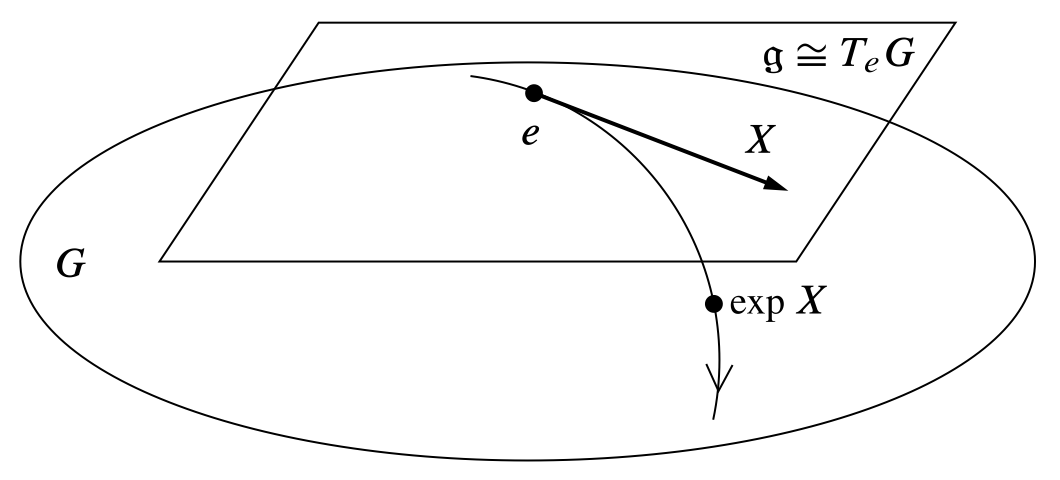
\includegraphics[width=0.7\linewidth]{exp}
	\label{fig:exp}
\end{figure}

\begin{prop}
	Let $G$ be a Lie group. For any $X\in\operatorname{Lie}(G)$, $\gamma(s)=\operatorname{exp} sX$ is the one-parameter subgroup of $G$ generated by $X$.
\end{prop}
\begin{example}\leavevmode
	\begin{enumerate}
		\item $\operatorname{exp} A=e^A$.
		\item If $V$ is any finite-dimensional real vector space, a choice of basis for $V$ yields isomorphisms $\operatorname{GL}(V)\cong\operatorname{GL}(n,\mathbb{R})$ and $\mathfrak{gl}(V)\cong\mathfrak{gl}(n,\mathbb{R})$. The analysis of the $\operatorname{GL}(n,\mathbb{R})$ case then shows that the exponential map of $\operatorname{GL}(V)$ can be written in the form
		\[\operatorname{exp} A=\sum_{k=0}^\infty\frac{1}{k!}A^k\]
		when we consider $A\in\mathfrak{gl}(V)$ as a linear map from $V$ to itself and $A^k=A\circ\ldots\circ A$.
	\end{enumerate}
\end{example}
\begin{prop}
	Let $G$ be a Lie group and $\mathfrak{g}$ be its Lie algebra.
	\begin{enumerate}
		\item The exponential map is a smooth map from $\mathfrak{g}$ to $G$.
		\item For any $X\in\mathfrak{g}$ and $s,t\in\mathbb{R}$, $\operatorname{exp}(s+t)X=\operatorname{exp} sX\operatorname{exp} tX$.
		\item For any $X\in\mathfrak{g}$, $(\operatorname{exp} X)^{-1}=\operatorname{exp}(-X)$.
		\item For any $X\in\mathfrak{g}$ and $n\in \mathbb{Z}$, $(\operatorname{exp} X)^n=\operatorname{exp}(nX)$.
		\item The differential $(d\operatorname{exp})_0:T_0\mathfrak{g}\to T_eG$ is the identity map, under the canonical identifications of both $T_0\mathfrak{g}$ and $T_eG$ with $\mathfrak{g}$ itself.
		\item The exponential map restricts to a diffeomorphism from some neighborhood of 0 in $\mathfrak{g}$ to a neighborhood of $e$ in $G$.
	\end{enumerate}
\end{prop}
Notice that $\operatorname{exp}(X+Y)=\operatorname{exp} X\operatorname{exp} Y$ for arbitrary $X,Y$ in the Lie algebra. In fact, for connected groups, this is only true when the group is abelian.

\begin{thm}[The Lie correspondence]
	There is a one-to-one correspondence between isomorphism classes of finite-dimensional Lie algebras and isomorphism classes of simply connected Lie groups given by associating each simply connected Lie group with its Lie algebra.
\end{thm}


\section{\(\mathsf{U}(n)\) is intersection of any two…}

 \paragraph{Problem 6:} Consider the standard compatible triple $(\operatorname{O}mega_0,J_0,g_0)$ on $\mathbb{R}^{2n}$. Let $\operatorname{O}(2n)$ be the linear orthogonal group of $\mathbb{R}^{2n}$ (i.e., linear transformations preserving the canonical inner product $g_0$), and let $\operatorname{Sp}(2n)$ be the symplectic linear group. Through the identification $\mathbb{R}^{2n}\cong \mathbb{C}^{n}$ (as complex vector spaces), we may see $\operatorname{GL}(n,\mathbb{C})$ (the group of linear automorphisms of $\mathbb{C}^{n}$) as a subgroup of $\operatorname{GL}(2n,\mathbb{R})$ : a complex matrix $A+iB$ is identified with the real $2n\times 2n$ matrix
 \[\begin{pmatrix}A&-B\\B&A\end{pmatrix}\]
Let now $\operatorname{U}(n)\subset\operatorname{GL}(n,\mathbb{C})$ be the group of linear transformation preserving the natural hermitian inner product of $\mathbb{C}^{n}$. Show that the intersection of any two of the groups
\[\operatorname{Sp}(2n),\operatorname{O}(2n),\operatorname{GL}(n,\mathbb{C})\subset\operatorname{GL}(2n,\mathbb{R})\]
is $\operatorname{U}(n)$.

\section{a fact about lie groups and flows}

Not sure where to put this so maybe here for now…

\begin{thing7}{Adjoint representation}\leavevmode
The \textit{\textbf{adjoint representation}} of a Lie group \(G\) is a map \(\operatorname{Ad}:G \to \mathsf{GL}(\mathfrak{g})\) that represents \(G\) as a group of linear automorphisms of its Lie algebra. It is given by \(G \ni a \mapsto (dC_a)_e\), the differential of the conjugation map \(C_a\).
\end{thing7}

\subsection*{flow of left-invariant is right multiplication}

Now I know what is a flow: the flow is
\[\varphi^t(p)\]
For every point of the manifold I get the integral curve of a vector field (of course a priori a flow is just a flow but let me just think it's the flow of a vector field). At every point you get a curve.

Now. The thing with the Lie bracket is that when you differentiate the flow you get to the Lie bracket via a formula that is hard to write. So the easy way to write it is:
\[[V,W]=\frac{d}{dt}\Big|_{t=0} \varphi^{-t}_{*,\varphi^t(p)}W_{\varphi^t(p)}\]
and that's it.

Now I will prove in Portuguese that \textbf{the flow of a left-invariant vector field is right-translation}. First I need a claim.

	\begin{claim}\leavevmode
	O fluxo \(\varphi\) de um campo invariante à esquerda \(w\) comuta com a traslação à esquerda, i.e.,
	\[\varphi_t(e)\circ L_h = L_h \circ \varphi_t(e)\qquad \forall t\in \mathbb{R} \forall h \in G.\]
	\end{claim}
	\begin{proof}[Prova da afirmação]\leavevmode
Derivamos de ambos lados. Por um lado,
\begin{align*}
\frac{d}{dt}\Big|_{t=0}\varphi_t(e) \circ L_h=\frac{d}{dt}\Big|_{t=0}\varphi_t(h)&=v_h\end{align*}
Por outro lado,
\[\frac{d}{dt}\Big|_{t=0}L_h \circ \varphi_t(e)=(L_h)_{*,\varphi_t(e)}\frac{d}{dt}\Big|_{t=0}\varphi_t(e)=(L_h)_{*,e}v_e=v_h.\]
Por unicidade das soluções de EDOs, acabou.
	\end{proof}
Então repare:
\[\varphi_t(h)=(\varphi_t\circ L_h)(e)=(L_h \circ \varphi_t)(e)=h\varphi_t(e)=R_{\varphi_t(e)}h,\]
ou seja, qualquer curva integral de \(w\) é simplesmente a curva integral que passa por \(e\) trasladada. \textbf{That's what I wanted to show but there's more:} 

Agora lembre que o colchete de Lie pode ser expressado como
\[[w,v]_e=\frac{d}{dt}\Big|_{t=0}\Big(\varphi_{-t}\Big)_{*,\varphi_t(e)}v_{\varphi_t(e)}.\]
(Onde fixamos o parámetro \(-t\) e deixamos livre o outro para ver \(\varphi_{-t}\) como um difeomorfismo de \(G\).)

Juntando com a discussão anterior obtemos
\[[w,v]_e=\frac{d}{dt}\Big|_{t=0}\Big(R_{\varphi_{-t}(e)}\Big)_{*,\varphi_t(e)}v_{\varphi_t(e)}.\]


\chapter{physics}

\section{a problem}
is that gravity and qm fail at a very basic observation: vacuum energy

quantization of a simple variational problem, for a scalar field, says that energy of the vacum is infinite. but there's an experiment that says that the cosmological constant (which is energy of the vacuum) is \(\rho_{cc}\approx 5 \times 10 ^{-10}\frac{J}{m^3}\).

The functional is
\begin{align*}
S&=\int dt \int d^3x \frac{1}{2}\left\{ \frac{1}{2}\dot\varphi^2-(\nabla \varphi)^2-m^2\varphi^2\right\} 
\end{align*}

we wish to experimentally find a system that is governed both by quantum mechanics and relativity. Experiment micro g by aspa-mayer shows gravitational laws in a 1-milimeter, i.e. \(10^{-6}\) kg particles. The size of the proton is about \(10^{-27}\) Kg, here you get quantum mechanics. People at puc have experiments with things of sizes \(10^{-18}\) Kg.

gr: the mass determines the metric


another problem: gravitational field and quantum superposition. two quantum states give two stress-energy tensors that produce two metrics via Einstein-Hilbert action. but there's some problem with this---
\bibliography{bib.bib}

\end{document}
